\documentclass[twoside]{book}

% Packages required by doxygen
\usepackage{fixltx2e}
\usepackage{calc}
\usepackage{doxygen}
\usepackage[export]{adjustbox} % also loads graphicx
\usepackage{graphicx}
\usepackage[utf8]{inputenc}
\usepackage{makeidx}
\usepackage{multicol}
\usepackage{multirow}
\PassOptionsToPackage{warn}{textcomp}
\usepackage{textcomp}
\usepackage[nointegrals]{wasysym}
\usepackage[table]{xcolor}

% Font selection
\usepackage[T1]{fontenc}
\usepackage[scaled=.90]{helvet}
\usepackage{courier}
\usepackage{amssymb}
\usepackage{sectsty}
\renewcommand{\familydefault}{\sfdefault}
\allsectionsfont{%
  \fontseries{bc}\selectfont%
  \color{darkgray}%
}
\renewcommand{\DoxyLabelFont}{%
  \fontseries{bc}\selectfont%
  \color{darkgray}%
}
\newcommand{\+}{\discretionary{\mbox{\scriptsize$\hookleftarrow$}}{}{}}

% Page & text layout
\usepackage{geometry}
\geometry{%
  a4paper,%
  top=2.5cm,%
  bottom=2.5cm,%
  left=2.5cm,%
  right=2.5cm%
}
\tolerance=750
\hfuzz=15pt
\hbadness=750
\setlength{\emergencystretch}{15pt}
\setlength{\parindent}{0cm}
\setlength{\parskip}{3ex plus 2ex minus 2ex}
\makeatletter
\renewcommand{\paragraph}{%
  \@startsection{paragraph}{4}{0ex}{-1.0ex}{1.0ex}{%
    \normalfont\normalsize\bfseries\SS@parafont%
  }%
}
\renewcommand{\subparagraph}{%
  \@startsection{subparagraph}{5}{0ex}{-1.0ex}{1.0ex}{%
    \normalfont\normalsize\bfseries\SS@subparafont%
  }%
}
\makeatother

% Headers & footers
\usepackage{fancyhdr}
\pagestyle{fancyplain}
\fancyhead[LE]{\fancyplain{}{\bfseries\thepage}}
\fancyhead[CE]{\fancyplain{}{}}
\fancyhead[RE]{\fancyplain{}{\bfseries\leftmark}}
\fancyhead[LO]{\fancyplain{}{\bfseries\rightmark}}
\fancyhead[CO]{\fancyplain{}{}}
\fancyhead[RO]{\fancyplain{}{\bfseries\thepage}}
\fancyfoot[LE]{\fancyplain{}{}}
\fancyfoot[CE]{\fancyplain{}{}}
\fancyfoot[RE]{\fancyplain{}{\bfseries\scriptsize Generated by Doxygen }}
\fancyfoot[LO]{\fancyplain{}{\bfseries\scriptsize Generated by Doxygen }}
\fancyfoot[CO]{\fancyplain{}{}}
\fancyfoot[RO]{\fancyplain{}{}}
\renewcommand{\footrulewidth}{0.4pt}
\renewcommand{\chaptermark}[1]{%
  \markboth{#1}{}%
}
\renewcommand{\sectionmark}[1]{%
  \markright{\thesection\ #1}%
}

% Indices & bibliography
\usepackage{natbib}
\usepackage[titles]{tocloft}
\setcounter{tocdepth}{3}
\setcounter{secnumdepth}{5}
\makeindex

% Hyperlinks (required, but should be loaded last)
\usepackage{ifpdf}
\ifpdf
  \usepackage[pdftex,pagebackref=true]{hyperref}
\else
  \usepackage[ps2pdf,pagebackref=true]{hyperref}
\fi
\hypersetup{%
  colorlinks=true,%
  linkcolor=blue,%
  citecolor=blue,%
  unicode%
}

% Custom commands
\newcommand{\clearemptydoublepage}{%
  \newpage{\pagestyle{empty}\cleardoublepage}%
}

\usepackage{caption}
\captionsetup{labelsep=space,justification=centering,font={bf},singlelinecheck=off,skip=4pt,position=top}

%===== C O N T E N T S =====

\begin{document}

% Titlepage & ToC
\hypersetup{pageanchor=false,
             bookmarksnumbered=true,
             pdfencoding=unicode
            }
\pagenumbering{alph}
\begin{titlepage}
\vspace*{7cm}
\begin{center}%
{\Large E\+HN 410 -\/ Group 7 -\/ A\+ES Encryption \\[1ex]\large 1.\+0 }\\
\vspace*{1cm}
{\large Generated by Doxygen 1.8.13}\\
\end{center}
\end{titlepage}
\clearemptydoublepage
\pagenumbering{roman}
\tableofcontents
\clearemptydoublepage
\pagenumbering{arabic}
\hypersetup{pageanchor=true}

%--- Begin generated contents ---
\chapter{R\+E\+A\+D\+ME}
\label{md__r_e_a_d_m_e}
\Hypertarget{md__r_e_a_d_m_e}


 \section*{E\+HN 410 -\/ Group 7}







 \subsection*{Group members\+:}




\begin{DoxyItemize}
\item Mohamed Ameen Omar (u16055323)
\item Douglas Healy (u16018100)
\item Llewellyn Moyse (u15100708)
\end{DoxyItemize}



 \subsection*{To run Encryption Platform}




\begin{DoxyEnumerate}
\item Open a Linux Terminal.
\item Navigate to the Encyption Platform Directory.
\item Run the \char`\"{}make\char`\"{} command.
\item An executable called \char`\"{}encyption\+Platform\char`\"{} will be created.
\item Use \char`\"{}./encyption\+Platform\char`\"{} to run the encryption platform. (if no input parameters are specified, a help menu will be displayed)
\item A list of input parameter and default values\+:
\end{DoxyEnumerate}

\tabulinesep=1mm
\begin{longtabu} spread 0pt [c]{*{3}{|X[-1]}|}
\hline
\rowcolor{\tableheadbgcolor}\textbf{ Parameter }&\textbf{ Description }&\textbf{ Default Value  }\\\cline{1-3}
\endfirsthead
\hline
\endfoot
\hline
\rowcolor{\tableheadbgcolor}\textbf{ Parameter }&\textbf{ Description }&\textbf{ Default Value  }\\\cline{1-3}
\endhead
-\/h &Print out the help menu &\\\cline{1-3}
-\/f or --filename &Path to an A\+S\+C\+II file to encrypt/decrypt &None \\\cline{1-3}
-\/F &Path to a hex file to encrypt/decrypt &None \\\cline{1-3}
-\/k or --key &The encryption key &128 bit N\+U\+LL key \\\cline{1-3}
-\/K &The encryption key (in hex) &None \\\cline{1-3}
-\/i or --IV &The Initialisation vector &128 bit N\+U\+LL IV \\\cline{1-3}
-\/I &The Initialisation vector (in hex) &None \\\cline{1-3}
-\/p or --plaintext &Plaintext to encrypt &None \\\cline{1-3}
-\/P &Plaintext to encrypt (in hex) &None \\\cline{1-3}
-\/c or --ciphertext &Ciphertext to decrypt &None \\\cline{1-3}
-\/C &Ciphertext to decrypt (in hex) &None \\\cline{1-3}
-\/m or --mode &Mode of encryption/decryption (ecb, cbc or cfb) &ecb \\\cline{1-3}
-\/v or --verbose &Print verbose output &Flag not set \\\cline{1-3}
-\/e or --encrypt &Encrypt plaintext or file &Flag set \\\cline{1-3}
-\/d or --decrypt &Decrypt ciphertext or file &Flag not set \\\cline{1-3}
-\/T &Set if input text is a hex string &Flag not set \\\cline{1-3}
\end{longtabu}
\#\# File Encryption Example 
\begin{DoxyCode}
./encryptionPlatform -e -f <path/unencrypted\_file.ext> -k <key> -i <iv>
./encryptionPlatform -e -F <path/unencrypted\_hex\_file.ext> -K <hex\_key> -I <hex\_iv>
\end{DoxyCode}


\subsection*{File Encryption Example}


\begin{DoxyCode}
./encryptionPlatform -d -f <path/encrypted\_file.ext> -k <key> -i <iv>
./encryptionPlatform -d -F <path/encrypted\_hex\_file.ext> -F <hex\_key> -I <hex\_iv>
\end{DoxyCode}
 
\chapter{File Index}
\section{File List}
Here is a list of all documented files with brief descriptions\+:\begin{DoxyCompactList}
\item\contentsline{section}{\hyperlink{_a_e_s_8c}{A\+E\+S.\+c} \\*A\+ES encryption and decryption module implementation file. This file contains the implementation of the functions used for A\+ES encryption and decryption. Input must be A\+S\+C\+II and not hex. The functions implemented in this file, perform the A\+ES encryption and decryption on a single block of size dictated by the variable A\+E\+S\+\_\+\+B\+L\+O\+C\+K\+\_\+\+S\+I\+ZE }{\pageref{_a_e_s_8c}}{}
\item\contentsline{section}{\hyperlink{_a_e_s_8h}{A\+E\+S.\+h} \\*A\+ES encryption and decryption module header file. This file contains the function headers for the functions used for A\+ES encryption and decryption. Input must be A\+S\+C\+II and not hex. The functions implemented in this file, perform the A\+ES encryption and decryption on a single block of size dictated by the variable A\+E\+S\+\_\+\+B\+L\+O\+C\+K\+\_\+\+S\+I\+ZE }{\pageref{_a_e_s_8h}}{}
\item\contentsline{section}{\hyperlink{aes_tester_8c}{aes\+Tester.\+c} \\*Main file }{\pageref{aes_tester_8c}}{}
\item\contentsline{section}{\hyperlink{cbc_8c}{cbc.\+c} \\*Cipher Block Chaining (C\+BC) -\/ A\+ES Implementation file This file contains the implementation of the functions used for the C\+BC mode of A\+ES encryption. This system supports both file and user input encryption, as hex or ascii input. If the user inputs data to be encrypted or decrypted, the result will be printed to the terminal, whereas if the user specifies a file to be encrypted or decrypted, a new file will be created and the result will be written to the file. The C\+BC Encryption platform encrypts and decrypts blocks 16 bytes at a time, using 0 padding. The IV is limited to 16 bytes and the key is limited to 32 bytes as per the A\+ES encryption standard }{\pageref{cbc_8c}}{}
\item\contentsline{section}{\hyperlink{cbc_8h}{cbc.\+h} \\*Cipher Block Chaining (C\+BC) -\/ A\+ES Header file This file contains the function headers of the functions used for the C\+BC mode of A\+ES encryption. This system supports both file and user input encryption, as hex or ascii input. If the user inputs data to be encrypted or decrypted, the result will be printed to the terminal, whereas if the user specifies a file to be encrypted or decrypted, a new file will be created and the result will be written to the file. The C\+BC Encryption platform encrypts and decrypts blocks 16 bytes at a time, using 0 padding. The IV is limited to 16 bytes and the key is limited to 32 bytes as per the A\+ES encryption standard }{\pageref{cbc_8h}}{}
\item\contentsline{section}{\hyperlink{cbc_tester_8c}{cbc\+Tester.\+c} \\*Main file }{\pageref{cbc_tester_8c}}{}
\item\contentsline{section}{\hyperlink{cfb_8c}{cfb.\+c} \\*Cipher Feedback (C\+FB) -\/ A\+ES implementation file This file contains the implementation of the functions used for the C\+FB mode of A\+ES encryption. This system supports both file and user input encryption, as hex or ascii input. If the user inputs data to be encrypted or decrypted, the result will be printed to the terminal, whereas if the user specifies a file to be encrypted or decrypted, a new file will be created and the result will be written to the file. The C\+FB Encryption platform encrypts and decrypts blocks 16 bytes at a time, using 0 padding }{\pageref{cfb_8c}}{}
\item\contentsline{section}{\hyperlink{cfb_8h}{cfb.\+h} \\*Cipher Feedback (C\+FB) -\/ A\+ES header file This file contains the function headers of the functions used for the C\+FB mode of A\+ES encryption. This system supports both file and user input encryption, as hex or ascii input. If the user inputs data to be encrypted or decrypted, the result will be printed to the terminal, whereas if the user specifies a file to be encrypted or decrypted, a new file will be created and the result will be written to the file. The C\+FB Encryption platform encrypts and decrypts blocks 16 bytes at a time, using 0 padding }{\pageref{cfb_8h}}{}
\item\contentsline{section}{\hyperlink{cfb_tester_8c}{cfb\+Tester.\+c} \\*Main file }{\pageref{cfb_tester_8c}}{}
\item\contentsline{section}{\hyperlink{ecb_8c}{ecb.\+c} \\*Electronic code book (E\+CB) -\/ A\+ES Implementation file This file contains the implementation of the functions used for the E\+CB mode of A\+ES encryption. This system supports both file and user input encryption, as hex or ascii input. If the user inputs data to be encrypted or decrypted, the result will be printed to the terminal, whereas if the user specifies a file to be encrypted or decrypted, a new file will be created and the result will be written to the file. The E\+CB Encryption platform encrypts and decrypts blocks 16 bytes at a time, using 0 padding }{\pageref{ecb_8c}}{}
\item\contentsline{section}{\hyperlink{ecb_8h}{ecb.\+h} \\*Electronic code book (E\+CB) -\/ A\+ES header file This file contains the function headers of the functions used for the E\+CB mode of A\+ES encryption. This system supports both file and user input encryption, as hex or ascii input. If the user inputs data to be encrypted or decrypted, the result will be printed to the terminal, whereas if the user specifies a file to be encrypted or decrypted, a new file will be created and the result will be written to the file. The E\+CB Encryption platform encrypts and decrypts blocks 16 bytes at a time, using 0 padding }{\pageref{ecb_8h}}{}
\item\contentsline{section}{{\bfseries ecb\+Tester.\+c} }{\pageref{ecb_tester_8c}}{}
\item\contentsline{section}{\hyperlink{encryption_platform_8c}{encryption\+Platform.\+c} \\*Implementation file for the cbc and cfb encryption platform. All functions, to specify key, IV, type of encrytion mode, file path or string controlled by commandline parameters }{\pageref{encryption_platform_8c}}{}
\item\contentsline{section}{{\bfseries encryption\+Platform.\+h} }{\pageref{encryption_platform_8h}}{}
\item\contentsline{section}{{\bfseries main.\+c} }{\pageref{main_8c}}{}
\item\contentsline{section}{{\bfseries my\+Tester.\+c} }{\pageref{my_tester_8c}}{}
\end{DoxyCompactList}

\chapter{File Documentation}
\hypertarget{_a_e_s_8c}{}\section{A\+E\+S.\+c File Reference}
\label{_a_e_s_8c}\index{A\+E\+S.\+c@{A\+E\+S.\+c}}


A\+ES encryption and decryption module implementation file. This file contains the implementation of the functions used for A\+ES encryption and decryption. Input must be A\+S\+C\+II and not hex. The functions implemented in this file, perform the A\+ES encryption and decryption on a single block of size dictated by the variable A\+E\+S\+\_\+\+B\+L\+O\+C\+K\+\_\+\+S\+I\+ZE.  


{\ttfamily \#include \char`\"{}A\+E\+S.\+h\char`\"{}}\newline
Include dependency graph for A\+E\+S.\+c\+:\nopagebreak
\begin{figure}[H]
\begin{center}
\leavevmode
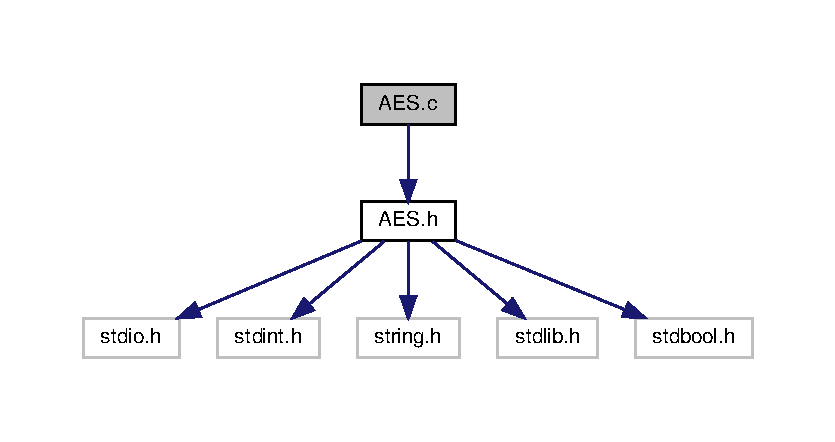
\includegraphics[width=350pt]{_a_e_s_8c__incl}
\end{center}
\end{figure}
\subsection*{Functions}
\begin{DoxyCompactItemize}
\item 
int \hyperlink{_a_e_s_8c_a1c2a403d95a85400bbae142d48cb8c9d}{get\+Num\+Rounds} (int key\+Length)
\begin{DoxyCompactList}\small\item\em get\+Num\+Rounds -\/ Function to return the number of rounds of A\+ES encryption and decryption based off of the length of the key given in \end{DoxyCompactList}\item 
unsigned char \hyperlink{_a_e_s_8c_acdf4abe2846c02b4d3e674782807fdfa}{get\+S\+Box\+Value} (unsigned char index)
\begin{DoxyCompactList}\small\item\em get\+S\+Box\+Value -\/ Function to return the s\+Box value passed in as a parameter \end{DoxyCompactList}\item 
unsigned char \hyperlink{_a_e_s_8c_a425f9b1e2cd595f2c45f129bc5d0a6d0}{get\+Inv\+S\+Box} (unsigned char index)
\begin{DoxyCompactList}\small\item\em get\+Inv\+S\+Box -\/ Function to return the inverse s\+Box value passed in as a parameter \end{DoxyCompactList}\item 
unsigned char \hyperlink{_a_e_s_8c_a4e58d2e928429bc56387394251b8ece5}{get\+Rcon\+Value} (unsigned char num)
\begin{DoxyCompactList}\small\item\em get\+Rcon\+Value -\/ Function to return the Rcon value for the index passed in as a parameter \end{DoxyCompactList}\item 
int \hyperlink{_a_e_s_8c_a5d65eac115e562c64b00a43e72ee6aca}{get\+Padded\+Key\+Length} (int current\+Key\+Length)
\begin{DoxyCompactList}\small\item\em get\+Padded\+Key\+Length -\/ Function to return a valid key length (in bytes) based off of the current key length passed in as \end{DoxyCompactList}\item 
unsigned char $\ast$ \hyperlink{_a_e_s_8c_a41cef4df290905c4d632ce1357d0a9bd}{A\+E\+S\+Encrypt} (unsigned char $\ast$plain\+Text, unsigned char $\ast$key, int plain\+Text\+Length, int key\+Length)
\begin{DoxyCompactList}\small\item\em A\+E\+S\+Encrypt -\/ Function to encrypt a single block of plaintext passed in as parameter  plain\+Text using A\+ES encryption, for 128, 192 and 256 bit keys. Validates the keylength and returns the corresponding ciphertext. The caller of the function must ensure that the returned ciphertext pointer is freed. The ciphertext returned is always 16 bytes and the plain\+Text must be 16 bytes or less. Makes use of zero padding. All input must be in A\+S\+C\+II and N\+OT hex. \end{DoxyCompactList}\item 
unsigned char $\ast$ \hyperlink{_a_e_s_8c_ab51c63e6483f94f12bbc9b256374ec64}{A\+E\+S\+Decrypt} (unsigned char $\ast$cipher\+Text, unsigned char $\ast$key, int cipher\+Text\+Length, int key\+Length)
\begin{DoxyCompactList}\small\item\em A\+E\+S\+Decrypt -\/ Function to decrypt a single block of ciphertext passed in as parameter  cipher\+Text using A\+ES decryption, for 128, 192 and 256 bit keys. Validates the keylength and returns the corresponding plaintext. The caller of the function must ensure that the returned plaintext pointer is freed. The plaintext returned is always 16 bytes and the plain\+Text must be 16 bytes or less. Makes use of zero padding. All input must be in A\+S\+C\+II and N\+OT hex. \end{DoxyCompactList}\item 
unsigned char $\ast$ \hyperlink{_a_e_s_8c_a185c827e4ccbc8e4608e83dfbf9dfc8e}{Rijndael\+Key\+Schedule} (unsigned char $\ast$original\+Key, int key\+Length)
\begin{DoxyCompactList}\small\item\em Rijndael\+Key\+Schedule -\/ Function that performs the Rijndael key scheduling for A\+ES encryption. Takes in the original key passed in as parameter. \end{DoxyCompactList}\item 
void \hyperlink{_a_e_s_8c_af2f914cf17729a0ee89102c98b39665e}{Key\+Schedule\+Core} (unsigned char $\ast$word, int word\+Length, int r\+Con\+Iteration\+Val)
\begin{DoxyCompactList}\small\item\em Key\+Schedule\+Core -\/ Function that performs the key schedule core for the Rijndael Key Schedule. Performs a single rotate left of the word passed in as. \end{DoxyCompactList}\item 
void \hyperlink{_a_e_s_8c_ac769b0533ccecd203cc3ab64e6b2f950}{Single\+Rotate\+Left} (unsigned char $\ast$word, int word\+Length)
\begin{DoxyCompactList}\small\item\em Single\+Rotate\+Left -\/ Function to rotate the array passed in as a paramter. \end{DoxyCompactList}\item 
void \hyperlink{_a_e_s_8c_ae9af90db32afa65125a7eec339ed9d58}{print\+State\+Array} (uint8\+\_\+t state\+Array\mbox{[}4\mbox{]}\mbox{[}4\mbox{]})
\begin{DoxyCompactList}\small\item\em print\+State\+Array -\/ Function to print the state array to the terminal in hex format. \end{DoxyCompactList}\item 
void \hyperlink{_a_e_s_8c_aef4d8fc4282e3cc21708d25c0ec9ad06}{Add\+Round\+Key} (unsigned char state\mbox{[}4\mbox{]}\mbox{[}4\mbox{]}, unsigned char key\mbox{[}4\mbox{]}\mbox{[}4\mbox{]})
\begin{DoxyCompactList}\small\item\em Add\+Round\+Key -\/ Function that performs the Bitwise X\+OR between state and key as per A\+ES encryption. \end{DoxyCompactList}\item 
void \hyperlink{_a_e_s_8c_aca09b30896a351db6587639a1cc1bf0d}{mix\+Columns} (unsigned char state\mbox{[}4\mbox{]}\mbox{[}4\mbox{]})
\begin{DoxyCompactList}\small\item\em mix\+Columns -\/ Function that performs the Mix\+Columns step of A\+ES as specified by A\+ES encryption. \end{DoxyCompactList}\item 
void \hyperlink{_a_e_s_8c_a9de891875f23dd3dff8fe3f8e10ba3ad}{inv\+Mix\+Columns} (unsigned char state\mbox{[}4\mbox{]}\mbox{[}4\mbox{]})
\begin{DoxyCompactList}\small\item\em inv\+Mix\+Columns -\/ Function that does the inverse of the Mix Column Step for A\+ES Encryption. Performs the gallois field multiplication and the required X\+OR to the state passed in as a paramter \end{DoxyCompactList}\item 
unsigned char \hyperlink{_a_e_s_8c_a7dbbb13c3ab5608765b6d368eb9f4fe1}{gallois\+Field\+Mult} (unsigned char a, unsigned char b)
\begin{DoxyCompactList}\small\item\em gallois\+Field\+Mult -\/ Function to perform the Galois field multiplication operation required for the inverse mix columns and the mix columns operation of the A\+ES encryption and decryption processes. Returns the result of the multiplication. \end{DoxyCompactList}\item 
void \hyperlink{_a_e_s_8c_aec40f89d2cbf831fd0d5d5f1bfa616f5}{sub\+Bytes} (unsigned char state\mbox{[}4\mbox{]}\mbox{[}4\mbox{]})
\begin{DoxyCompactList}\small\item\em sub\+Bytes -\/ Function that performs the sub byte operation where each value is replaced by the s box value \end{DoxyCompactList}\item 
void \hyperlink{_a_e_s_8c_a8e72edc1f652f8626aacd2781303c86b}{inv\+Sub\+Bytes} (unsigned char state\mbox{[}4\mbox{]}\mbox{[}4\mbox{]})
\begin{DoxyCompactList}\small\item\em inv\+Sub\+Bytes -\/ Function that performs the inverse of Function sub\+Bytes \end{DoxyCompactList}\item 
void \hyperlink{_a_e_s_8c_abeb4dba64fcf4d07eac178e732ca6aa8}{Shift\+Rows} (unsigned char state\mbox{[}4\mbox{]}\mbox{[}4\mbox{]}, int word\+Length)
\begin{DoxyCompactList}\small\item\em Shift\+Rows -\/ Function to shift the state array according to the A\+ES encryption standard for 128 -\/ bits blocks. \end{DoxyCompactList}\item 
void \hyperlink{_a_e_s_8c_a903e34d08dd07be2e2d9618d4d489ee6}{inv\+Shift\+Rows} (unsigned char state\mbox{[}4\mbox{]}\mbox{[}4\mbox{]}, int word\+Length)
\begin{DoxyCompactList}\small\item\em inv\+Shift\+Rows -\/ Function to shift the state array Inverse according to the A\+ES encryption standard for 128 -\/ bits blocks \end{DoxyCompactList}\item 
void \hyperlink{_a_e_s_8c_a4fc33ada95d0d2aaea28086aefe173bb}{Single\+Rotate\+Right} (unsigned char $\ast$word, int word\+Length)
\begin{DoxyCompactList}\small\item\em Single\+Rotate\+Right -\/ Function to rotate the array passed in as a paramter. \end{DoxyCompactList}\item 
void \hyperlink{_a_e_s_8c_abe15a731f43315f6f595674d3cd62d57}{get\+Round\+Key} (unsigned char $\ast$expanded\+Key, unsigned char $\ast$round\+Key, int round\+Num)
\begin{DoxyCompactList}\small\item\em get\+Round\+Key -\/ Function to extract the correct sub-\/key to use for the appropriate round specified by \end{DoxyCompactList}\item 
void \hyperlink{_a_e_s_8c_a1c1a633a58f7328faa397db9e45e7e0c}{construct\+State\+Array} (unsigned char $\ast$flat\+Array, unsigned char state\+Array\mbox{[}$\,$\mbox{]}\mbox{[}4\mbox{]})
\begin{DoxyCompactList}\small\item\em construct\+State\+Array -\/ Function to convert the state array from a flat 1D array to a multidimensional array. \end{DoxyCompactList}\item 
uint8\+\_\+t \hyperlink{_a_e_s_8c_a7e5ab2188af44718071074f450963568}{hex\+To\+Int} (char ch)
\begin{DoxyCompactList}\small\item\em hex\+To\+Int -\/ Function that converts a given hex value into an integer. \end{DoxyCompactList}\item 
uint8\+\_\+t \hyperlink{_a_e_s_8c_aa177516503b10de65b504a3714073ad7}{hex\+To\+Ascii} (char ch1, char ch2)
\begin{DoxyCompactList}\small\item\em hex\+To\+Ascii -\/ Function that converts a given hex value to its A\+S\+C\+II equivalent. \end{DoxyCompactList}\item 
void \hyperlink{_a_e_s_8c_ad697cbb5d9e462b3017df1f1d939ee96}{hex\+To\+Ascii\+String} (char $\ast$hex\+String, char $\ast$ascii\+String, int hex\+String\+Length)
\begin{DoxyCompactList}\small\item\em hex\+To\+Ascii\+String -\/ Function that converts a given string of hex values into its A\+S\+C\+II equivalent. A hex string contains hex chars and is \char`\"{}encoded\char`\"{} in ascii In order to encrypt it, it must be converted to the equivalent ascii plain text string plaintext string is half the size of hex, since two hex chars = 1 ascii char if hex string is \char`\"{}4\+A\char`\"{} it will be converted to \char`\"{}\+J\char`\"{} in ascii which will have a hex representation of \char`\"{}4a\char`\"{} The original hex string converted to hex staright or printed in hex straight rather will print or have the value \char`\"{}0x34\char`\"{}, \char`\"{}0x31\char`\"{} B\+A\+S\+I\+C\+A\+L\+LY T\+HE H\+EX S\+T\+R\+I\+NG FF IS I\+N\+T\+E\+R\+P\+R\+E\+T\+ED AS T\+HE C\+H\+A\+RS FF, whereas when using this function we intend it to be \char`\"{}\+J\char`\"{}, ie the char \char`\"{}\+J\char`\"{} \end{DoxyCompactList}\item 
unsigned char $\ast$ \hyperlink{_a_e_s_8c_ac189aee6672718650020cf627d45c780}{ascii\+To\+Hex\+String} (unsigned char $\ast$ascii\+String, unsigned char $\ast$hex\+String, size\+\_\+t ascii\+String\+Len)
\begin{DoxyCompactList}\small\item\em Function name\+: ascii\+To\+Hex\+String -\/ convert an ascii String to an ascii string. \end{DoxyCompactList}\item 
void \hyperlink{_a_e_s_8c_a0e0b199ded54d7fb53a3bda3fcc02256}{validate\+Num\+Rounds} (int num\+Rounds, int key\+Length)
\begin{DoxyCompactList}\small\item\em validate\+Num\+Rounds -\/ Function that validates the number of rounds that have been passed in by the \end{DoxyCompactList}\item 
void \hyperlink{_a_e_s_8c_acefcd728377e1e14187fa8fcd20f4064}{validate\+Plain\+Text\+Length} (size\+\_\+t plain\+Text\+Length)
\begin{DoxyCompactList}\small\item\em validate\+Plain\+Text\+Length -\/ Function that validates the length of the plaintext. The validation is done against the A\+E\+S\+\_\+\+B\+L\+O\+C\+K\+\_\+\+S\+I\+ZE value \end{DoxyCompactList}\item 
void \hyperlink{_a_e_s_8c_ae01a1e7833d53f19b534e37ace03a691}{validate\+Cipher\+Text\+Length} (int cipher\+Text\+Length)
\begin{DoxyCompactList}\small\item\em validate\+Cipher\+Text\+Length -\/ Function that validates the length of the ciphertext. The validation is done against the A\+E\+S\+\_\+\+B\+L\+O\+C\+K\+\_\+\+S\+I\+ZE value \end{DoxyCompactList}\item 
void \hyperlink{_a_e_s_8c_aaba2e1b9466483b3c6b8669eb42aa5ed}{print\+A\+E\+S\+Block} (unsigned char $\ast$block)
\begin{DoxyCompactList}\small\item\em print\+A\+E\+S\+Block -\/ Function to print a single block in hex format to the terminal. \end{DoxyCompactList}\item 
int \hyperlink{_a_e_s_8c_a9dcad0047890de22f3d15611a10ab74f}{file\+Name\+Dir\+Index} (char $\ast$file\+Name, int file\+Name\+Length)
\begin{DoxyCompactList}\small\item\em Returns the last index of \textquotesingle{}/\textquotesingle{} in a given path, otherwise returns -\/1 if no \textquotesingle{}/\textquotesingle{} is found. \end{DoxyCompactList}\item 
void \hyperlink{_a_e_s_8c_ab066697b473ad5ce74faaceae6def5e5}{strip\+Directory} (char $\ast$file\+Name, char $\ast$extracted\+File\+Name, char $\ast$extracted\+File\+Path, int file\+Name\+Length, int slash\+Index)
\begin{DoxyCompactList}\small\item\em Removes path from the provided path to a file and returns only the file name. \end{DoxyCompactList}\item 
void \hyperlink{_a_e_s_8c_acc2acf0b03a8863f9290bdd36dd6f478}{get\+Output\+File\+Name} (int type, char $\ast$file\+Name, char $\ast$output\+File\+Name, char $\ast$mode)
\begin{DoxyCompactList}\small\item\em Get the output file name from all the parameters passed in. \end{DoxyCompactList}\item 
uint8\+\_\+t \hyperlink{_a_e_s_8c_a3bf513612c15693c3b2be10b94298e05}{is\+File\+Txt} (unsigned char $\ast$file\+Name)
\begin{DoxyCompactList}\small\item\em is\+File\+Txt -\/ Function to determine if the file passed in as a paramter \end{DoxyCompactList}\item 
unsigned char $\ast$ \hyperlink{_a_e_s_8c_afba897e91364663f883cc51ed309dc92}{key\+Hex\+To\+Ascii} (unsigned char $\ast$hex\+Key, int key\+Length)
\begin{DoxyCompactList}\small\item\em key\+Hex\+To\+Ascii -\/ Function to convert a key from a Hex string passed in as a paramter \end{DoxyCompactList}\item 
unsigned char $\ast$ \hyperlink{_a_e_s_8c_ad82d1b77336ac1292ed5a24b92380f42}{I\+V\+Hex\+To\+Ascii} (unsigned char $\ast$hex\+IV, int I\+V\+Length)
\begin{DoxyCompactList}\small\item\em I\+V\+Hex\+To\+Ascii -\/ Function to convert a initialization vector from a Hex string passed in as a paramter. \end{DoxyCompactList}\item 
unsigned char $\ast$ \hyperlink{_a_e_s_8c_ab601c369ba50730fc02d03bc44aad4e0}{X\+O\+R\+Blocks} (unsigned char $\ast$block1, unsigned char $\ast$block2, int length)
\begin{DoxyCompactList}\small\item\em X\+O\+R\+Blocks -\/ Function to X\+OR two blocks of length. \end{DoxyCompactList}\end{DoxyCompactItemize}
\subsection*{Variables}
\begin{DoxyCompactItemize}
\item 
const size\+\_\+t \hyperlink{_a_e_s_8c_ac3c0558617e372fc5ce3648e041e549c}{A\+E\+S\+\_\+\+B\+L\+O\+C\+K\+\_\+\+S\+I\+ZE} = 16
\begin{DoxyCompactList}\small\item\em Variable-\/ const size\+\_\+t A\+E\+S\+\_\+\+B\+L\+O\+C\+K\+\_\+\+S\+I\+ZE. Used to dictate the length in bytes of a single A\+ES block used for encryption and decryption. Set to 16 bytes for a single block. \end{DoxyCompactList}\item 
size\+\_\+t \hyperlink{_a_e_s_8c_a48113b3faee8aad8efa17aac0b56b63b}{V\+E\+R\+B\+O\+SE} = 0
\begin{DoxyCompactList}\small\item\em Variable-\/ size\+\_\+t V\+E\+R\+B\+O\+SE Used to dictate whether verbose output is printed to the terminal or not. If 0, does not print verbose. If 1, prints verbose. \end{DoxyCompactList}\item 
const unsigned char \hyperlink{_a_e_s_8c_abbb6f385c467cfd964a68eeb6caaa04f}{sbox} \mbox{[}256\mbox{]}
\begin{DoxyCompactList}\small\item\em const unsigned char sbox. Lookup table for the sbox values used during A\+ES Encryption. \end{DoxyCompactList}\item 
const unsigned char \hyperlink{_a_e_s_8c_afdaefaa3b28b23dc18709335449a1427}{inv\+S\+Box} \mbox{[}256\mbox{]}
\begin{DoxyCompactList}\small\item\em const unsigned char inv\+S\+Box. Lookup table for the inverse sbox values used during A\+ES Decryption. \end{DoxyCompactList}\item 
const unsigned char \hyperlink{_a_e_s_8c_a58c62505f9b71b2c257046ccf4c9153c}{Rcon} \mbox{[}255\mbox{]}
\begin{DoxyCompactList}\small\item\em const unsigned char Rcon. Lookup table for the Rcon values used during Rijndael Key Schedule during the A\+ES Encryption and Decryption. \end{DoxyCompactList}\end{DoxyCompactItemize}


\subsection{Detailed Description}
A\+ES encryption and decryption module implementation file. This file contains the implementation of the functions used for A\+ES encryption and decryption. Input must be A\+S\+C\+II and not hex. The functions implemented in this file, perform the A\+ES encryption and decryption on a single block of size dictated by the variable A\+E\+S\+\_\+\+B\+L\+O\+C\+K\+\_\+\+S\+I\+ZE. 

\begin{DoxyAuthor}{Authors}
Mohamed Ameen Omar (u16055323) 

Douglas Healy (u16018100) 

Llewellyn Moyse (u15100708) 
\end{DoxyAuthor}
\begin{DoxyVersion}{Version}
0.\+1 
\end{DoxyVersion}
\begin{DoxyDate}{Date}
2019-\/03-\/20
\end{DoxyDate}
\begin{DoxyCopyright}{Copyright}
Copyright (c) 2019 
\end{DoxyCopyright}


\subsection{Function Documentation}
\mbox{\Hypertarget{_a_e_s_8c_aef4d8fc4282e3cc21708d25c0ec9ad06}\label{_a_e_s_8c_aef4d8fc4282e3cc21708d25c0ec9ad06}} 
\index{A\+E\+S.\+c@{A\+E\+S.\+c}!Add\+Round\+Key@{Add\+Round\+Key}}
\index{Add\+Round\+Key@{Add\+Round\+Key}!A\+E\+S.\+c@{A\+E\+S.\+c}}
\subsubsection{\texorpdfstring{Add\+Round\+Key()}{AddRoundKey()}}
{\footnotesize\ttfamily void Add\+Round\+Key (\begin{DoxyParamCaption}\item[{unsigned char}]{state\mbox{[}4\mbox{]}\mbox{[}4\mbox{]},  }\item[{unsigned char}]{key\mbox{[}4\mbox{]}\mbox{[}4\mbox{]} }\end{DoxyParamCaption})}



Add\+Round\+Key -\/ Function that performs the Bitwise X\+OR between state and key as per A\+ES encryption. 


\begin{DoxyParams}{Parameters}
{\em state} & -\/ unsigned char -\/ is the current state of the ciphertext or plaintext during A\+ES encryption or decryption \\
\hline
{\em key} & -\/ unsigned char -\/ sub key to be added for the current round to the current state vector \\
\hline
\end{DoxyParams}


Definition at line 688 of file A\+E\+S.\+c.

Here is the caller graph for this function\+:\nopagebreak
\begin{figure}[H]
\begin{center}
\leavevmode
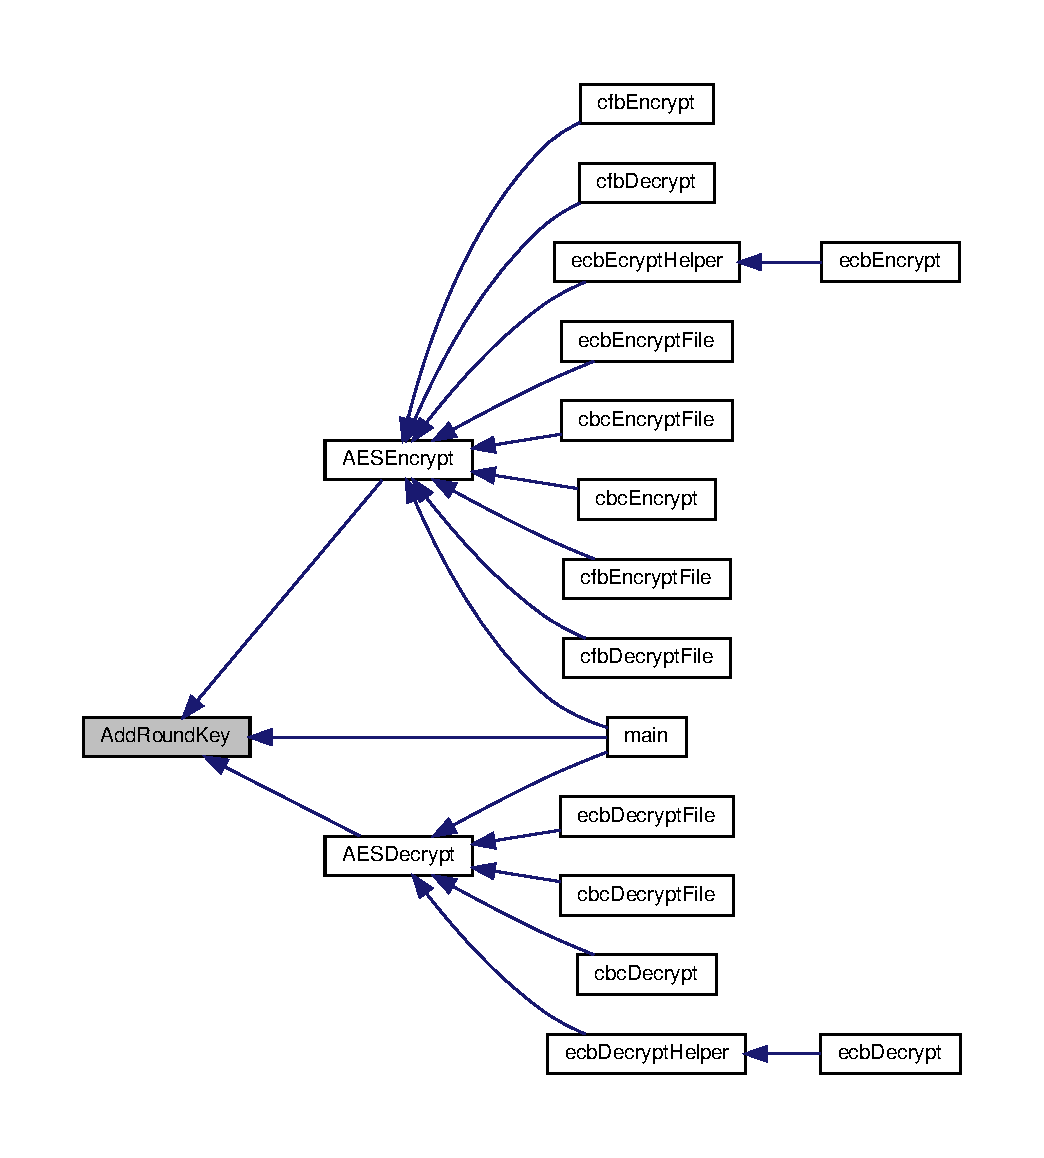
\includegraphics[width=350pt]{_a_e_s_8c_aef4d8fc4282e3cc21708d25c0ec9ad06_icgraph}
\end{center}
\end{figure}
\mbox{\Hypertarget{_a_e_s_8c_ab51c63e6483f94f12bbc9b256374ec64}\label{_a_e_s_8c_ab51c63e6483f94f12bbc9b256374ec64}} 
\index{A\+E\+S.\+c@{A\+E\+S.\+c}!A\+E\+S\+Decrypt@{A\+E\+S\+Decrypt}}
\index{A\+E\+S\+Decrypt@{A\+E\+S\+Decrypt}!A\+E\+S.\+c@{A\+E\+S.\+c}}
\subsubsection{\texorpdfstring{A\+E\+S\+Decrypt()}{AESDecrypt()}}
{\footnotesize\ttfamily unsigned char$\ast$ A\+E\+S\+Decrypt (\begin{DoxyParamCaption}\item[{unsigned char $\ast$}]{cipher\+Text,  }\item[{unsigned char $\ast$}]{key,  }\item[{int}]{cipher\+Text\+Length,  }\item[{int}]{key\+Length }\end{DoxyParamCaption})}



A\+E\+S\+Decrypt -\/ Function to decrypt a single block of ciphertext passed in as parameter  cipher\+Text using A\+ES decryption, for 128, 192 and 256 bit keys. Validates the keylength and returns the corresponding plaintext. The caller of the function must ensure that the returned plaintext pointer is freed. The plaintext returned is always 16 bytes and the plain\+Text must be 16 bytes or less. Makes use of zero padding. All input must be in A\+S\+C\+II and N\+OT hex. 


\begin{DoxyParams}{Parameters}
{\em char} & -\/ unsigned char$\ast$ cipher\+Text -\/ pointer to the ciphertext that needs to be decrypted using A\+ES decryption. \\
\hline
{\em char} & -\/ unsigned char$\ast$ key -\/ reference to the key that must be used for A\+ES decryption. \\
\hline
{\em cipher\+Text\+Length} & -\/ length of the ciphertext in \\
\hline
{\em cipher\+Text} & to be decrypted. \\
\hline
{\em key\+Length} & -\/ length of the key passed in as \\
\hline
{\em key} & used for the A\+ES decryption. \\
\hline
\end{DoxyParams}
\begin{DoxyReturn}{Returns}
unsigned$\ast$ char -\/ Plaintext resulting from the decryption of the ciphertext passed in as 
\end{DoxyReturn}

\begin{DoxyParams}{Parameters}
{\em cipher\+Text.} & \\
\hline
\end{DoxyParams}


Definition at line 399 of file A\+E\+S.\+c.

Here is the call graph for this function\+:\nopagebreak
\begin{figure}[H]
\begin{center}
\leavevmode
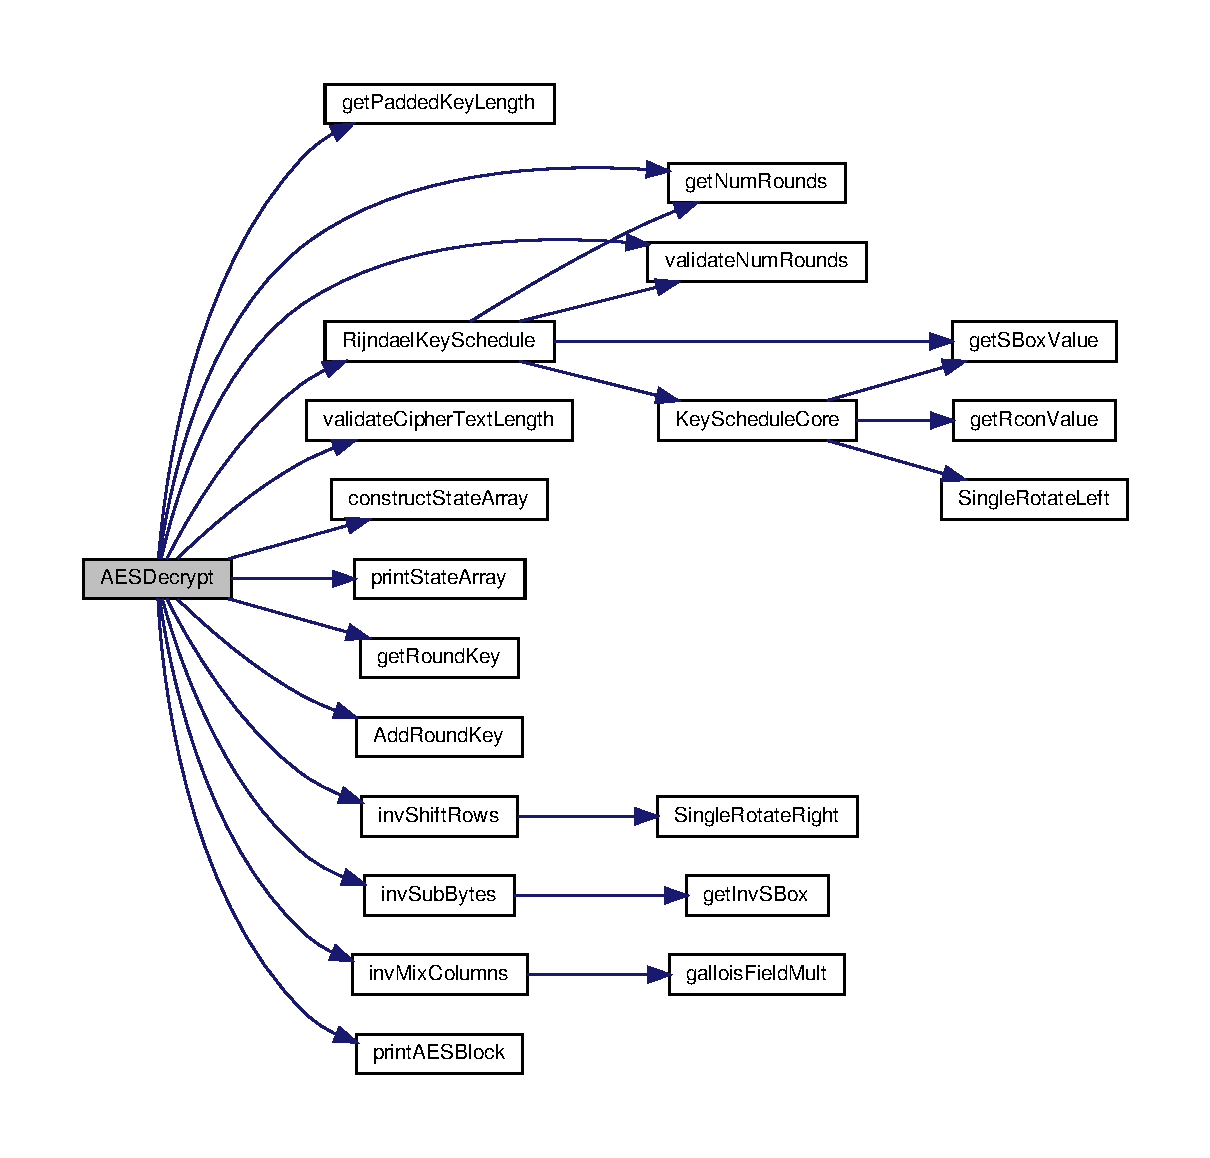
\includegraphics[width=350pt]{_a_e_s_8c_ab51c63e6483f94f12bbc9b256374ec64_cgraph}
\end{center}
\end{figure}
Here is the caller graph for this function\+:\nopagebreak
\begin{figure}[H]
\begin{center}
\leavevmode
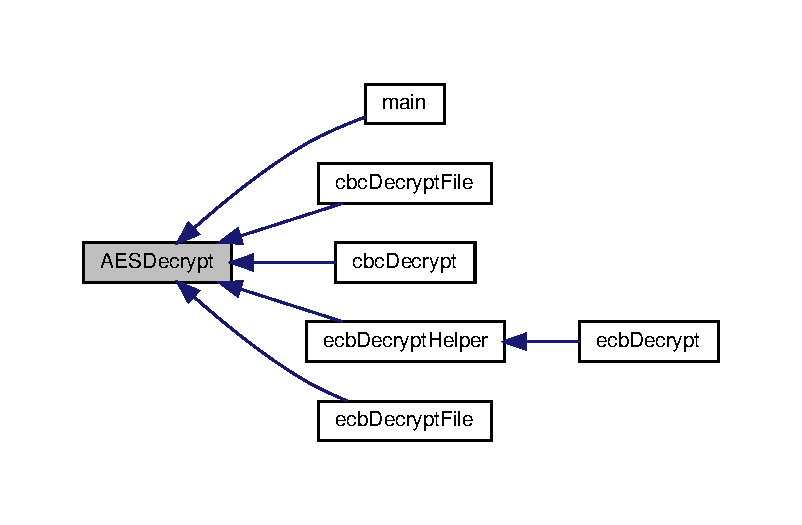
\includegraphics[width=350pt]{_a_e_s_8c_ab51c63e6483f94f12bbc9b256374ec64_icgraph}
\end{center}
\end{figure}
\mbox{\Hypertarget{_a_e_s_8c_a41cef4df290905c4d632ce1357d0a9bd}\label{_a_e_s_8c_a41cef4df290905c4d632ce1357d0a9bd}} 
\index{A\+E\+S.\+c@{A\+E\+S.\+c}!A\+E\+S\+Encrypt@{A\+E\+S\+Encrypt}}
\index{A\+E\+S\+Encrypt@{A\+E\+S\+Encrypt}!A\+E\+S.\+c@{A\+E\+S.\+c}}
\subsubsection{\texorpdfstring{A\+E\+S\+Encrypt()}{AESEncrypt()}}
{\footnotesize\ttfamily unsigned char$\ast$ A\+E\+S\+Encrypt (\begin{DoxyParamCaption}\item[{unsigned char $\ast$}]{plain\+Text,  }\item[{unsigned char $\ast$}]{key,  }\item[{int}]{plain\+Text\+Length,  }\item[{int}]{key\+Length }\end{DoxyParamCaption})}



A\+E\+S\+Encrypt -\/ Function to encrypt a single block of plaintext passed in as parameter  plain\+Text using A\+ES encryption, for 128, 192 and 256 bit keys. Validates the keylength and returns the corresponding ciphertext. The caller of the function must ensure that the returned ciphertext pointer is freed. The ciphertext returned is always 16 bytes and the plain\+Text must be 16 bytes or less. Makes use of zero padding. All input must be in A\+S\+C\+II and N\+OT hex. 


\begin{DoxyParams}{Parameters}
{\em char} & -\/ unsigned char$\ast$ plain\+Text -\/ pointer to the plaintext that needs to be encrypted using A\+ES encryption. \\
\hline
{\em char} & -\/ unsigned char$\ast$ key -\/ reference to the key that must be used for A\+ES encryption. \\
\hline
{\em plain\+Text\+Length} & -\/ length of the plaintext in \\
\hline
{\em plain\+Text} & to be encrypted. \\
\hline
{\em key\+Length} & -\/ length of the key passed in as \\
\hline
{\em key} & used for the A\+ES encryption. \\
\hline
\end{DoxyParams}
\begin{DoxyReturn}{Returns}
unsigned$\ast$ char -\/ Ciphertext resulting from the encryption of the plaintext passed in as 
\end{DoxyReturn}

\begin{DoxyParams}{Parameters}
{\em plain\+Text.} & \\
\hline
\end{DoxyParams}


Definition at line 198 of file A\+E\+S.\+c.

Here is the call graph for this function\+:\nopagebreak
\begin{figure}[H]
\begin{center}
\leavevmode
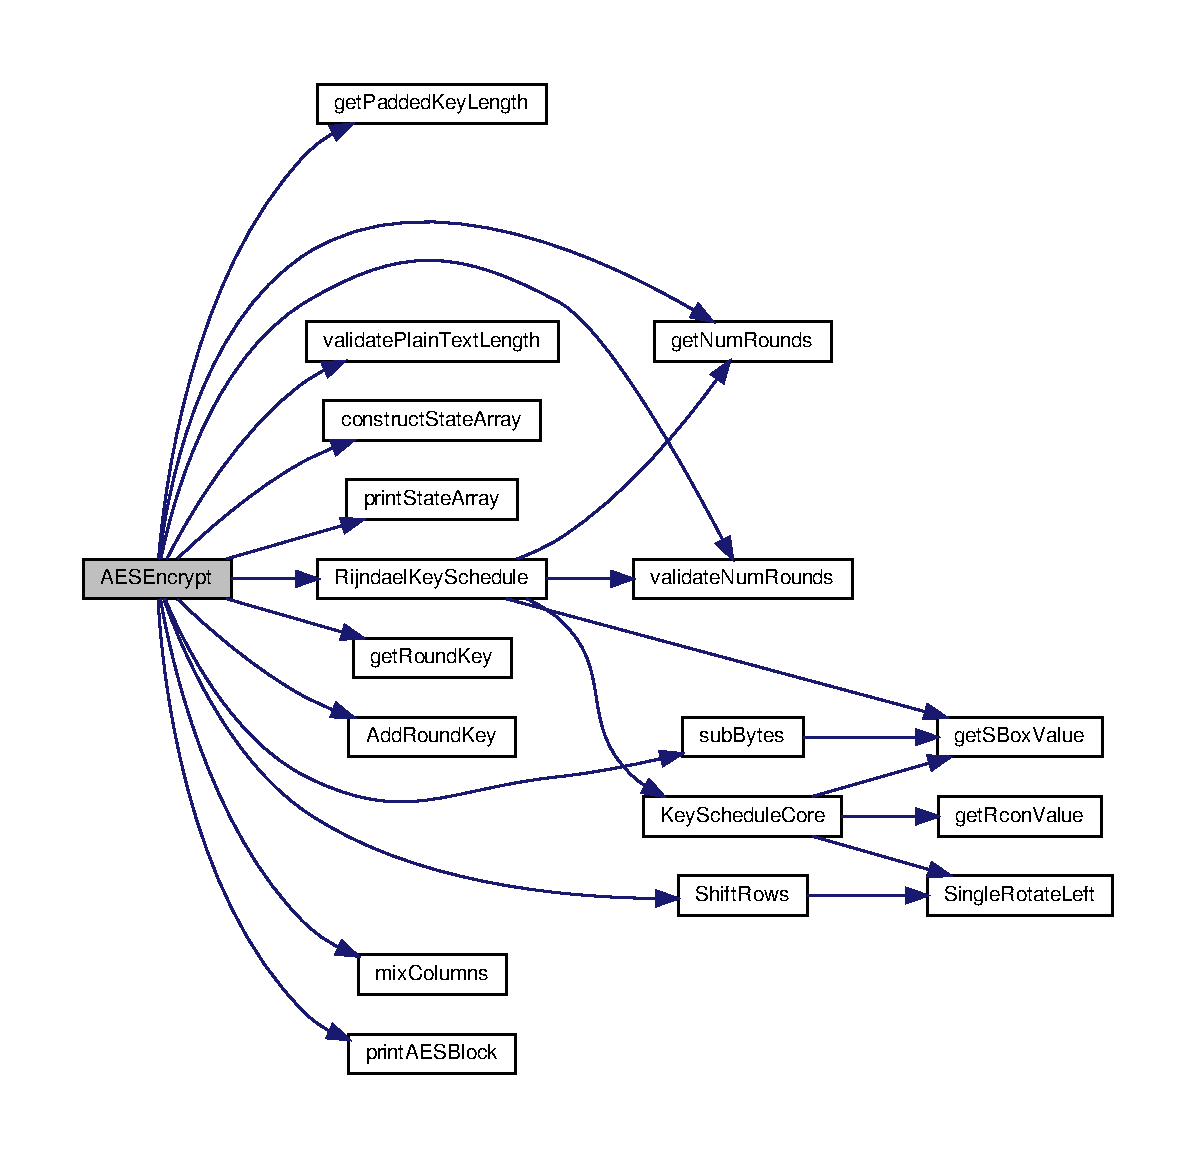
\includegraphics[width=350pt]{_a_e_s_8c_a41cef4df290905c4d632ce1357d0a9bd_cgraph}
\end{center}
\end{figure}
Here is the caller graph for this function\+:\nopagebreak
\begin{figure}[H]
\begin{center}
\leavevmode
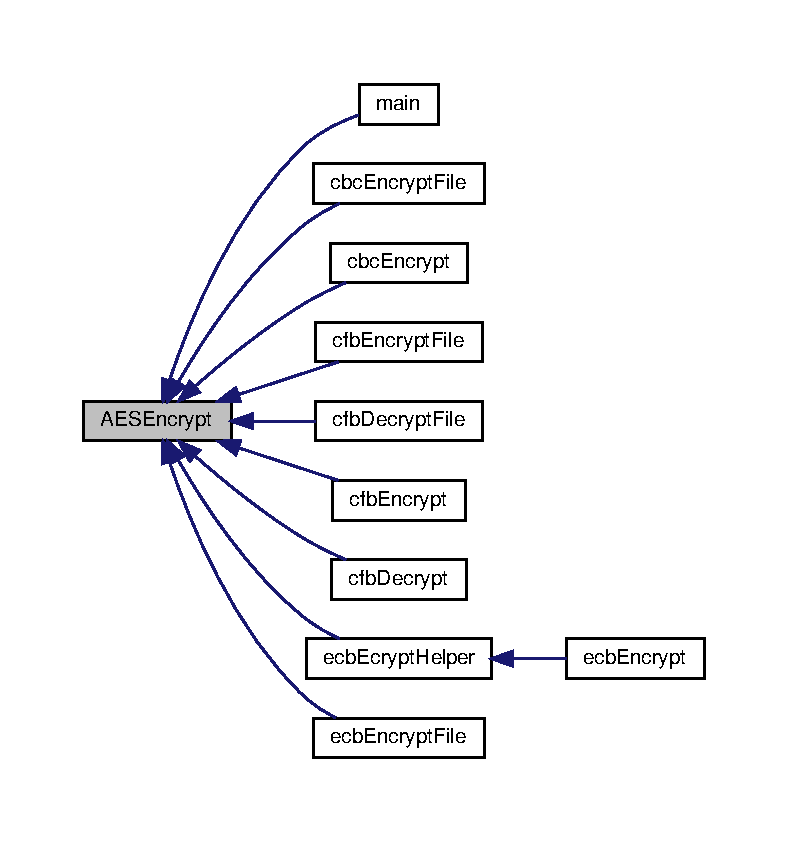
\includegraphics[width=350pt]{_a_e_s_8c_a41cef4df290905c4d632ce1357d0a9bd_icgraph}
\end{center}
\end{figure}
\mbox{\Hypertarget{_a_e_s_8c_ac189aee6672718650020cf627d45c780}\label{_a_e_s_8c_ac189aee6672718650020cf627d45c780}} 
\index{A\+E\+S.\+c@{A\+E\+S.\+c}!ascii\+To\+Hex\+String@{ascii\+To\+Hex\+String}}
\index{ascii\+To\+Hex\+String@{ascii\+To\+Hex\+String}!A\+E\+S.\+c@{A\+E\+S.\+c}}
\subsubsection{\texorpdfstring{ascii\+To\+Hex\+String()}{asciiToHexString()}}
{\footnotesize\ttfamily unsigned char$\ast$ ascii\+To\+Hex\+String (\begin{DoxyParamCaption}\item[{unsigned char $\ast$}]{ascii\+String,  }\item[{unsigned char $\ast$}]{hex\+String,  }\item[{size\+\_\+t}]{ascii\+String\+Len }\end{DoxyParamCaption})}



Function name\+: ascii\+To\+Hex\+String -\/ convert an ascii String to an ascii string. 


\begin{DoxyParams}{Parameters}
{\em ascii\+String} & -\/ unsigned char$\ast$ pointing to the A\+S\+C\+II String to be converted. \\
\hline
{\em hex\+String} & -\/ unsigned char$\ast$ pointing to a memory where the converted Hex string should be stored. \\
\hline
{\em ascii\+String\+Len} & -\/ size\+\_\+t containing the length of the A\+S\+C\+II String to be converted. \\
\hline
\end{DoxyParams}
\begin{DoxyReturn}{Returns}
unsigned char$\ast$ ascii\+To\+Hex\+String -\/ pointer to the converted Hex String, pointing to the same memory location as 
\end{DoxyReturn}

\begin{DoxyParams}{Parameters}
{\em hex\+String.} & \\
\hline
\end{DoxyParams}


Definition at line 971 of file A\+E\+S.\+c.

Here is the caller graph for this function\+:\nopagebreak
\begin{figure}[H]
\begin{center}
\leavevmode
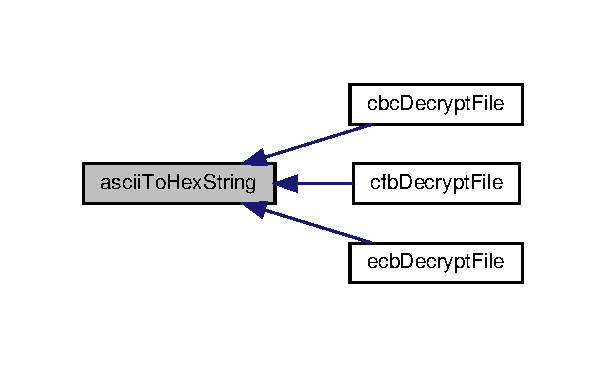
\includegraphics[width=291pt]{_a_e_s_8c_ac189aee6672718650020cf627d45c780_icgraph}
\end{center}
\end{figure}
\mbox{\Hypertarget{_a_e_s_8c_a1c1a633a58f7328faa397db9e45e7e0c}\label{_a_e_s_8c_a1c1a633a58f7328faa397db9e45e7e0c}} 
\index{A\+E\+S.\+c@{A\+E\+S.\+c}!construct\+State\+Array@{construct\+State\+Array}}
\index{construct\+State\+Array@{construct\+State\+Array}!A\+E\+S.\+c@{A\+E\+S.\+c}}
\subsubsection{\texorpdfstring{construct\+State\+Array()}{constructStateArray()}}
{\footnotesize\ttfamily void construct\+State\+Array (\begin{DoxyParamCaption}\item[{unsigned char $\ast$}]{flat\+Array,  }\item[{unsigned char}]{state\+Array\mbox{[}$\,$\mbox{]}\mbox{[}4\mbox{]} }\end{DoxyParamCaption})}



construct\+State\+Array -\/ Function to convert the state array from a flat 1D array to a multidimensional array. 


\begin{DoxyParams}{Parameters}
{\em char} & flat\+Array -\/the 1D array to be converted. \\
\hline
{\em state\+Array} & -\/ the multidimensional array to which to copy the flat array elements to. \\
\hline
\end{DoxyParams}


Definition at line 895 of file A\+E\+S.\+c.

Here is the caller graph for this function\+:\nopagebreak
\begin{figure}[H]
\begin{center}
\leavevmode
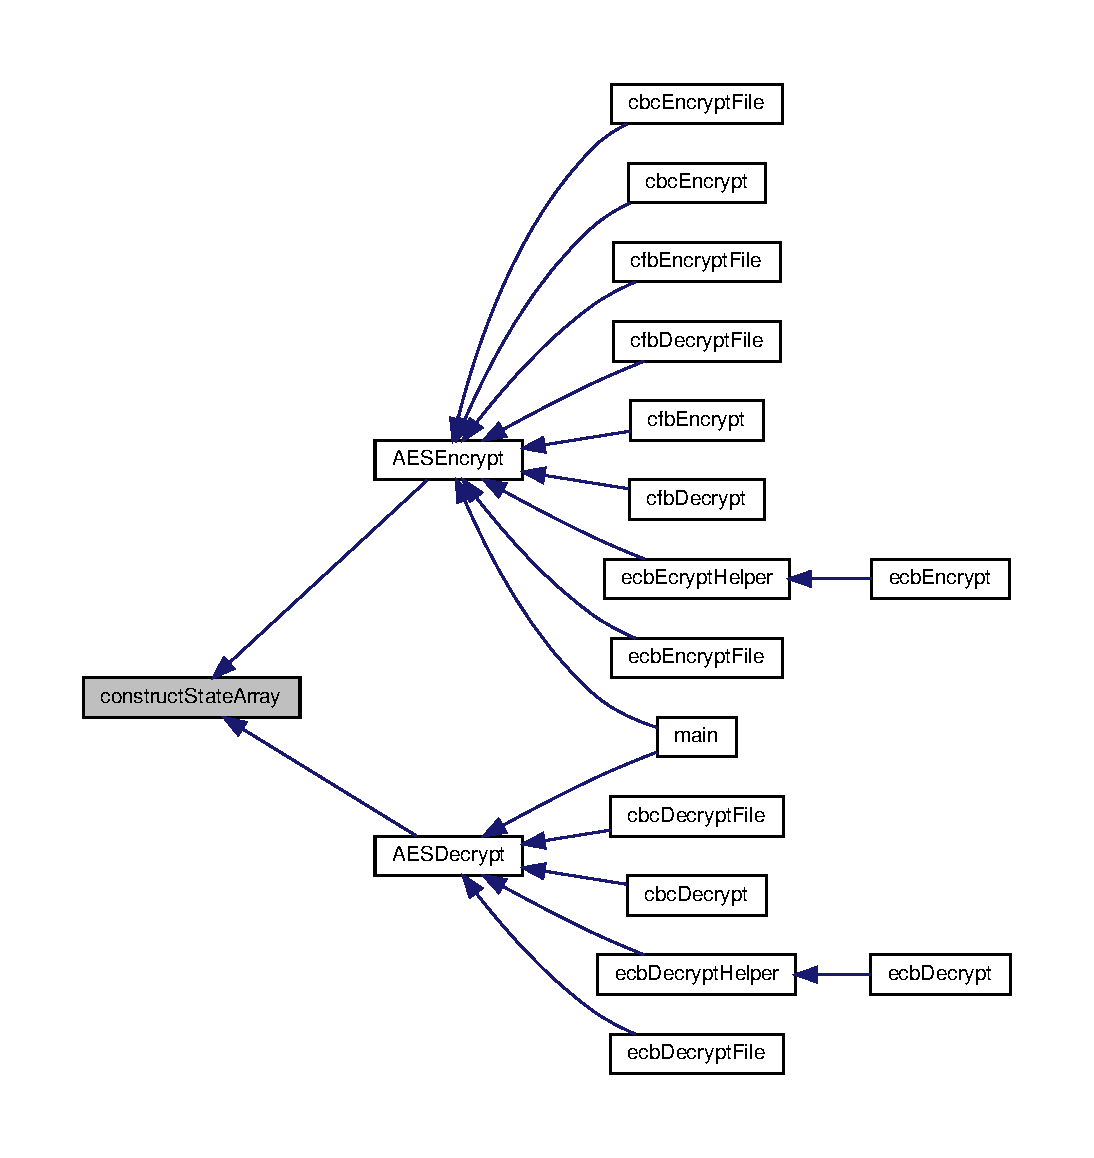
\includegraphics[width=350pt]{_a_e_s_8c_a1c1a633a58f7328faa397db9e45e7e0c_icgraph}
\end{center}
\end{figure}
\mbox{\Hypertarget{_a_e_s_8c_a9dcad0047890de22f3d15611a10ab74f}\label{_a_e_s_8c_a9dcad0047890de22f3d15611a10ab74f}} 
\index{A\+E\+S.\+c@{A\+E\+S.\+c}!file\+Name\+Dir\+Index@{file\+Name\+Dir\+Index}}
\index{file\+Name\+Dir\+Index@{file\+Name\+Dir\+Index}!A\+E\+S.\+c@{A\+E\+S.\+c}}
\subsubsection{\texorpdfstring{file\+Name\+Dir\+Index()}{fileNameDirIndex()}}
{\footnotesize\ttfamily int file\+Name\+Dir\+Index (\begin{DoxyParamCaption}\item[{char $\ast$}]{file\+Name,  }\item[{int}]{file\+Name\+Length }\end{DoxyParamCaption})}



Returns the last index of \textquotesingle{}/\textquotesingle{} in a given path, otherwise returns -\/1 if no \textquotesingle{}/\textquotesingle{} is found. 


\begin{DoxyParams}{Parameters}
{\em file\+Name} & The path to a file \\
\hline
{\em file\+Name\+Length} & The length of the provided file \\
\hline
\end{DoxyParams}
\begin{DoxyReturn}{Returns}
int Index of the last \textquotesingle{}/\textquotesingle{} in the path, else -\/1 if no \textquotesingle{}/\textquotesingle{} was found 
\end{DoxyReturn}


Definition at line 1043 of file A\+E\+S.\+c.

Here is the caller graph for this function\+:\nopagebreak
\begin{figure}[H]
\begin{center}
\leavevmode
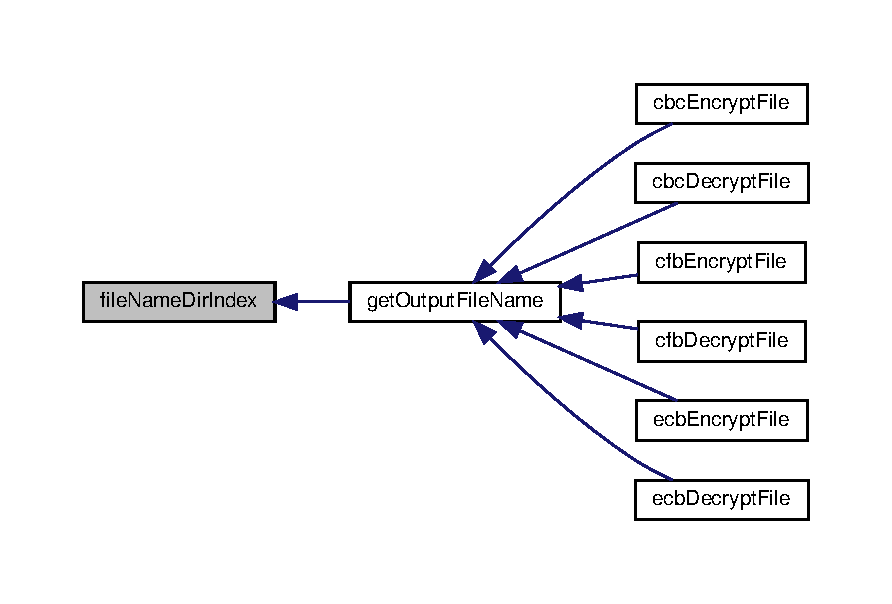
\includegraphics[width=350pt]{_a_e_s_8c_a9dcad0047890de22f3d15611a10ab74f_icgraph}
\end{center}
\end{figure}
\mbox{\Hypertarget{_a_e_s_8c_a7dbbb13c3ab5608765b6d368eb9f4fe1}\label{_a_e_s_8c_a7dbbb13c3ab5608765b6d368eb9f4fe1}} 
\index{A\+E\+S.\+c@{A\+E\+S.\+c}!gallois\+Field\+Mult@{gallois\+Field\+Mult}}
\index{gallois\+Field\+Mult@{gallois\+Field\+Mult}!A\+E\+S.\+c@{A\+E\+S.\+c}}
\subsubsection{\texorpdfstring{gallois\+Field\+Mult()}{galloisFieldMult()}}
{\footnotesize\ttfamily unsigned char gallois\+Field\+Mult (\begin{DoxyParamCaption}\item[{unsigned char}]{a,  }\item[{unsigned char}]{b }\end{DoxyParamCaption})}



gallois\+Field\+Mult -\/ Function to perform the Galois field multiplication operation required for the inverse mix columns and the mix columns operation of the A\+ES encryption and decryption processes. Returns the result of the multiplication. 


\begin{DoxyParams}{Parameters}
{\em a} & -\/ first character to perform Galois field multiplication. \\
\hline
{\em b} & -\/ second character to perform Galois field multiplication. \\
\hline
\end{DoxyParams}
\begin{DoxyReturn}{Returns}
unsigned char -\/ Result of the Galois field multiplication. 
\end{DoxyReturn}


Definition at line 764 of file A\+E\+S.\+c.

Here is the caller graph for this function\+:\nopagebreak
\begin{figure}[H]
\begin{center}
\leavevmode
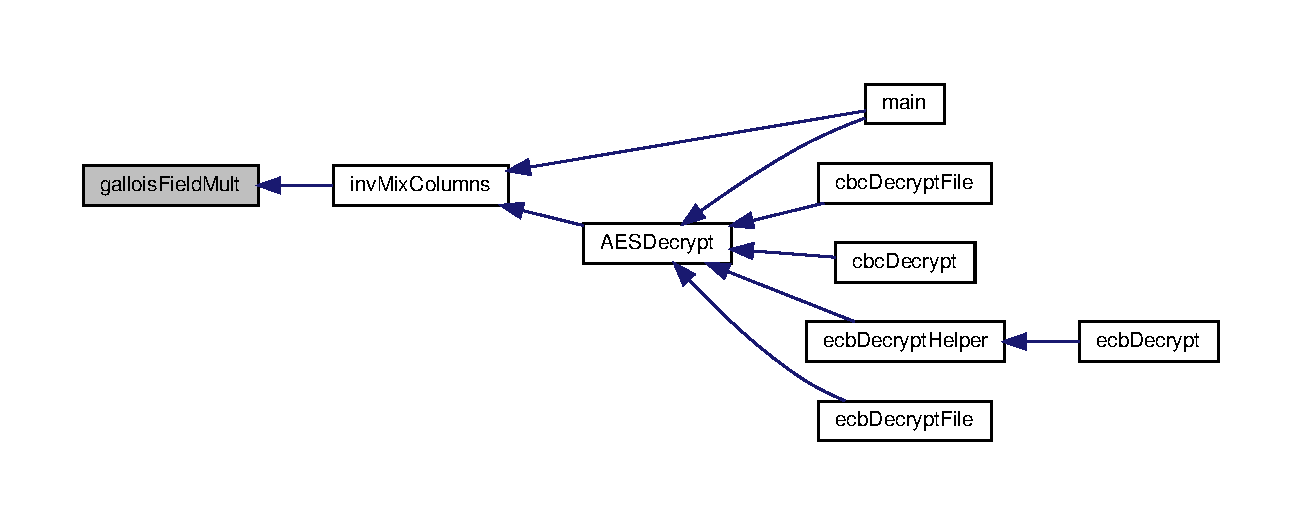
\includegraphics[width=350pt]{_a_e_s_8c_a7dbbb13c3ab5608765b6d368eb9f4fe1_icgraph}
\end{center}
\end{figure}
\mbox{\Hypertarget{_a_e_s_8c_a425f9b1e2cd595f2c45f129bc5d0a6d0}\label{_a_e_s_8c_a425f9b1e2cd595f2c45f129bc5d0a6d0}} 
\index{A\+E\+S.\+c@{A\+E\+S.\+c}!get\+Inv\+S\+Box@{get\+Inv\+S\+Box}}
\index{get\+Inv\+S\+Box@{get\+Inv\+S\+Box}!A\+E\+S.\+c@{A\+E\+S.\+c}}
\subsubsection{\texorpdfstring{get\+Inv\+S\+Box()}{getInvSBox()}}
{\footnotesize\ttfamily unsigned char get\+Inv\+S\+Box (\begin{DoxyParamCaption}\item[{unsigned char}]{index }\end{DoxyParamCaption})}



get\+Inv\+S\+Box -\/ Function to return the inverse s\+Box value passed in as a parameter 


\begin{DoxyParams}{Parameters}
{\em index.} & Requires the original value required in hex.\\
\hline
{\em index} & -\/ unsigned char -\/ hexadecimal representation of the index for which the inverse S\+Box value is required. \\
\hline
\end{DoxyParams}
\begin{DoxyReturn}{Returns}
unsigned char -\/ inverse s\+Box value for the paramter 
\end{DoxyReturn}

\begin{DoxyParams}{Parameters}
{\em index.} & \\
\hline
\end{DoxyParams}


Definition at line 146 of file A\+E\+S.\+c.

Here is the caller graph for this function\+:\nopagebreak
\begin{figure}[H]
\begin{center}
\leavevmode
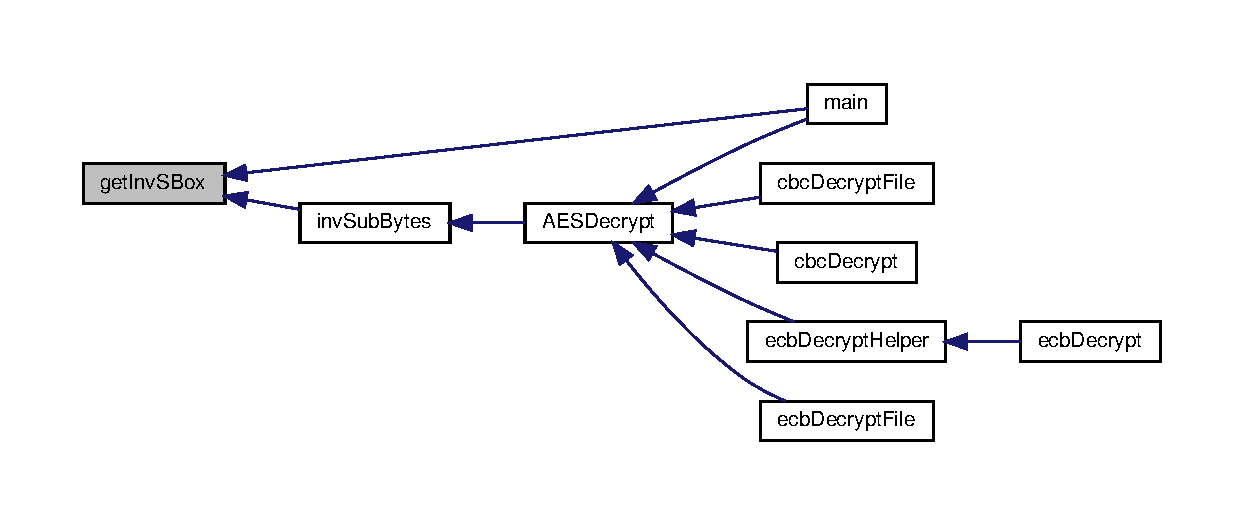
\includegraphics[width=350pt]{_a_e_s_8c_a425f9b1e2cd595f2c45f129bc5d0a6d0_icgraph}
\end{center}
\end{figure}
\mbox{\Hypertarget{_a_e_s_8c_a1c2a403d95a85400bbae142d48cb8c9d}\label{_a_e_s_8c_a1c2a403d95a85400bbae142d48cb8c9d}} 
\index{A\+E\+S.\+c@{A\+E\+S.\+c}!get\+Num\+Rounds@{get\+Num\+Rounds}}
\index{get\+Num\+Rounds@{get\+Num\+Rounds}!A\+E\+S.\+c@{A\+E\+S.\+c}}
\subsubsection{\texorpdfstring{get\+Num\+Rounds()}{getNumRounds()}}
{\footnotesize\ttfamily int get\+Num\+Rounds (\begin{DoxyParamCaption}\item[{int}]{key\+Length }\end{DoxyParamCaption})}



get\+Num\+Rounds -\/ Function to return the number of rounds of A\+ES encryption and decryption based off of the length of the key given in 


\begin{DoxyParams}{Parameters}
{\em key\+Length.} & \\
\hline
{\em key\+Length} & -\/ int -\/ indicates the length of the key \\
\hline
\end{DoxyParams}
\begin{DoxyReturn}{Returns}
int -\/ the number of rounds based off of the length of the key passed in the parameter 
\end{DoxyReturn}

\begin{DoxyParams}{Parameters}
{\em key\+Length.} & If the length of the key is not valid, returns -\/1. \\
\hline
\end{DoxyParams}


Definition at line 114 of file A\+E\+S.\+c.

Here is the caller graph for this function\+:\nopagebreak
\begin{figure}[H]
\begin{center}
\leavevmode
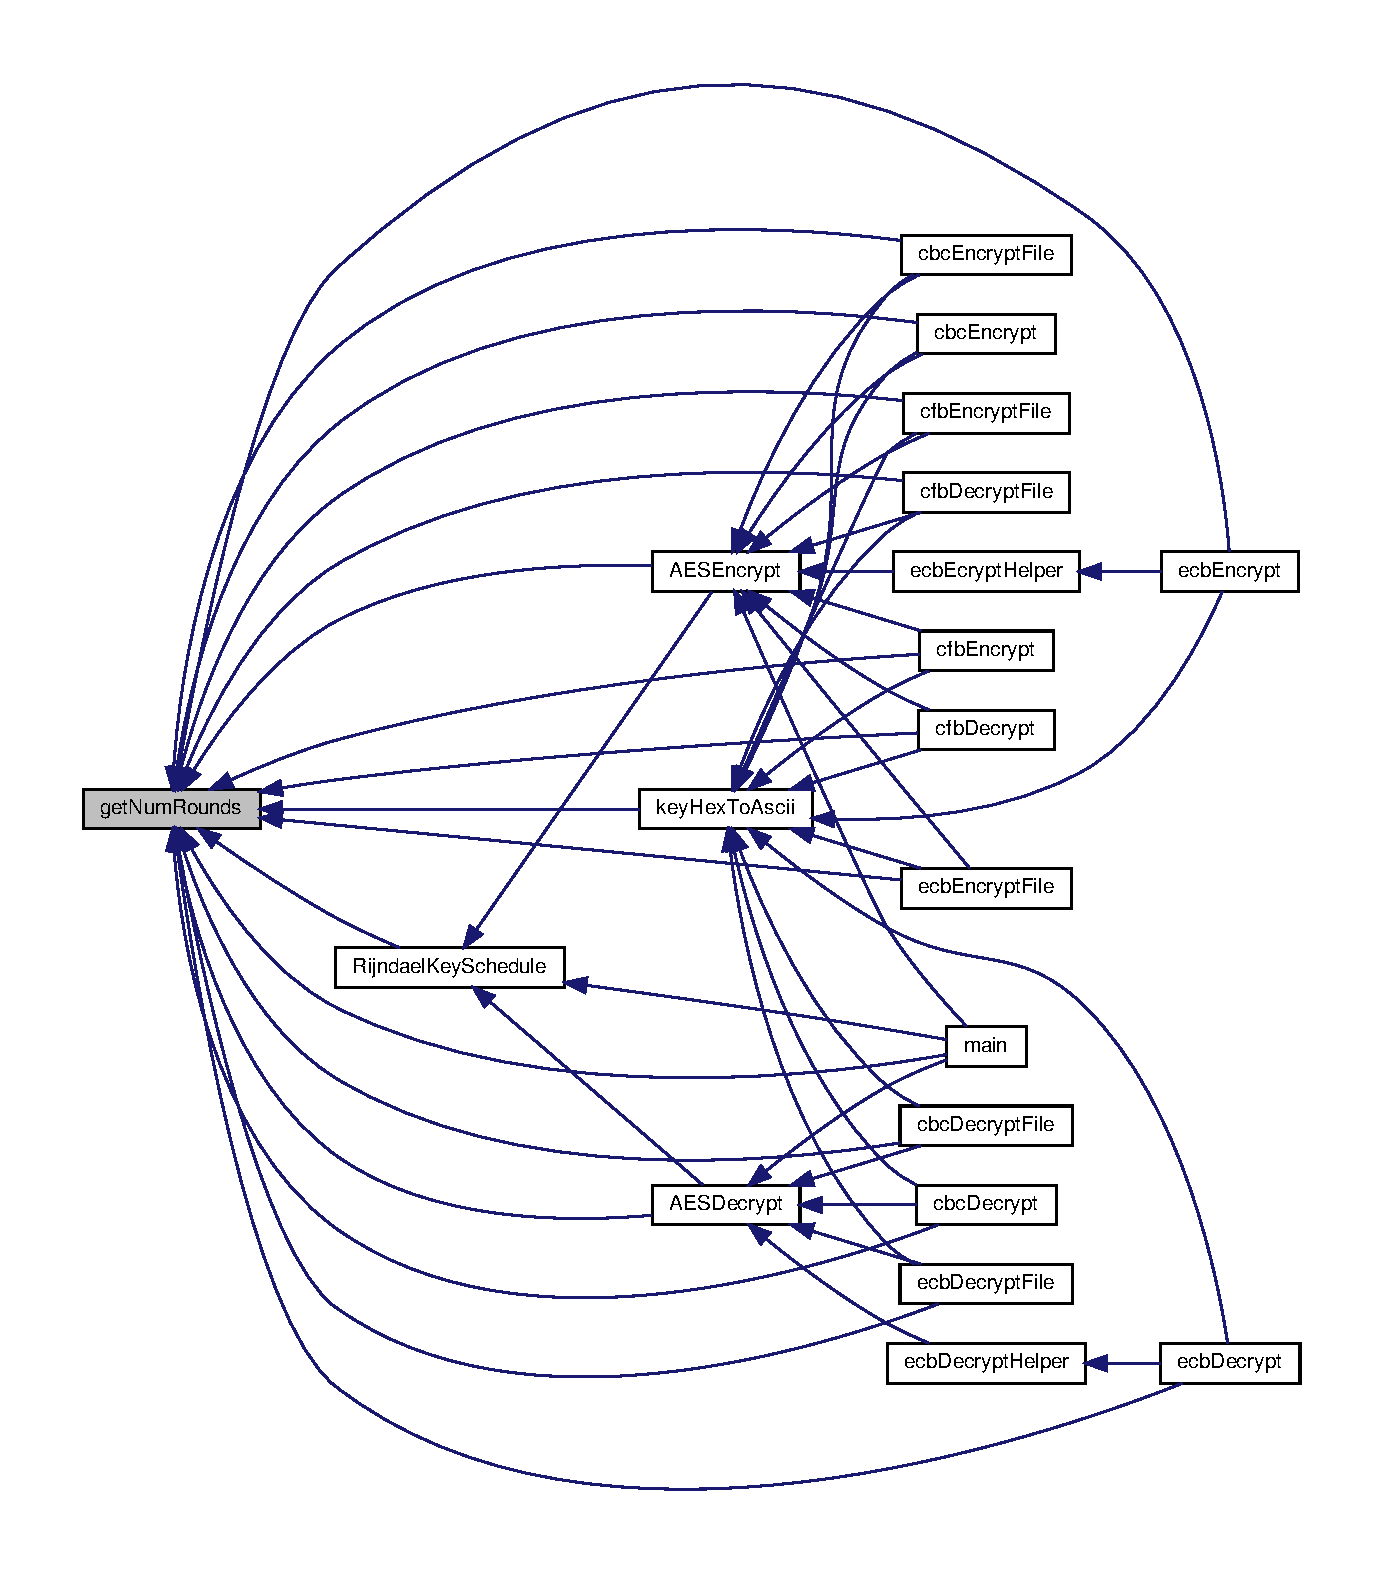
\includegraphics[width=350pt]{_a_e_s_8c_a1c2a403d95a85400bbae142d48cb8c9d_icgraph}
\end{center}
\end{figure}
\mbox{\Hypertarget{_a_e_s_8c_acc2acf0b03a8863f9290bdd36dd6f478}\label{_a_e_s_8c_acc2acf0b03a8863f9290bdd36dd6f478}} 
\index{A\+E\+S.\+c@{A\+E\+S.\+c}!get\+Output\+File\+Name@{get\+Output\+File\+Name}}
\index{get\+Output\+File\+Name@{get\+Output\+File\+Name}!A\+E\+S.\+c@{A\+E\+S.\+c}}
\subsubsection{\texorpdfstring{get\+Output\+File\+Name()}{getOutputFileName()}}
{\footnotesize\ttfamily void get\+Output\+File\+Name (\begin{DoxyParamCaption}\item[{int}]{type,  }\item[{char $\ast$}]{file\+Name,  }\item[{char $\ast$}]{output\+File\+Name,  }\item[{char $\ast$}]{mode }\end{DoxyParamCaption})}



Get the output file name from all the parameters passed in. 


\begin{DoxyParams}{Parameters}
{\em type} & 0 -\/ Encrypt, 1 -\/ Decrypt \\
\hline
{\em file\+Name} & The name of the input file \\
\hline
{\em output\+File\+Name} & The name of the output file \\
\hline
{\em mode} & Chipher mode to be used (E\+CB, C\+BC, C\+FB) \\
\hline
\end{DoxyParams}


Definition at line 1086 of file A\+E\+S.\+c.

Here is the call graph for this function\+:\nopagebreak
\begin{figure}[H]
\begin{center}
\leavevmode
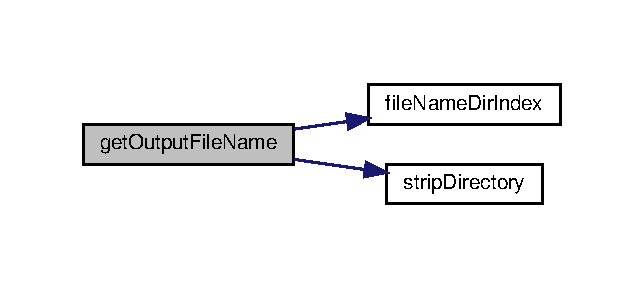
\includegraphics[width=309pt]{_a_e_s_8c_acc2acf0b03a8863f9290bdd36dd6f478_cgraph}
\end{center}
\end{figure}
Here is the caller graph for this function\+:\nopagebreak
\begin{figure}[H]
\begin{center}
\leavevmode
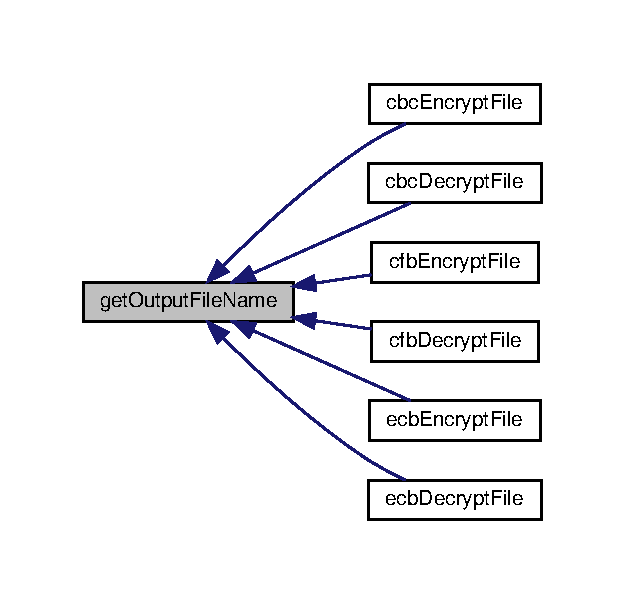
\includegraphics[width=300pt]{_a_e_s_8c_acc2acf0b03a8863f9290bdd36dd6f478_icgraph}
\end{center}
\end{figure}
\mbox{\Hypertarget{_a_e_s_8c_a5d65eac115e562c64b00a43e72ee6aca}\label{_a_e_s_8c_a5d65eac115e562c64b00a43e72ee6aca}} 
\index{A\+E\+S.\+c@{A\+E\+S.\+c}!get\+Padded\+Key\+Length@{get\+Padded\+Key\+Length}}
\index{get\+Padded\+Key\+Length@{get\+Padded\+Key\+Length}!A\+E\+S.\+c@{A\+E\+S.\+c}}
\subsubsection{\texorpdfstring{get\+Padded\+Key\+Length()}{getPaddedKeyLength()}}
{\footnotesize\ttfamily int get\+Padded\+Key\+Length (\begin{DoxyParamCaption}\item[{int}]{current\+Key\+Length }\end{DoxyParamCaption})}



get\+Padded\+Key\+Length -\/ Function to return a valid key length (in bytes) based off of the current key length passed in as 


\begin{DoxyParams}{Parameters}
{\em current\+Key\+Length.} & Corresponds to minimum and maximum key length required for A\+ES encryption and decryption. The key will then be padded to the length of the value returned from this function. If the keylength is less than 16, will return 16. If greater than 16, but less than 24, will return 24. If greater than 32, will return -\/1.\\
\hline
{\em current\+Key\+Length} & -\/ int -\/ current key length in bytes, to be padded to the return value \\
\hline
\end{DoxyParams}
\begin{DoxyReturn}{Returns}
int -\/ the length in bytes that the key should be padded to. 
\end{DoxyReturn}


Definition at line 172 of file A\+E\+S.\+c.

Here is the caller graph for this function\+:\nopagebreak
\begin{figure}[H]
\begin{center}
\leavevmode
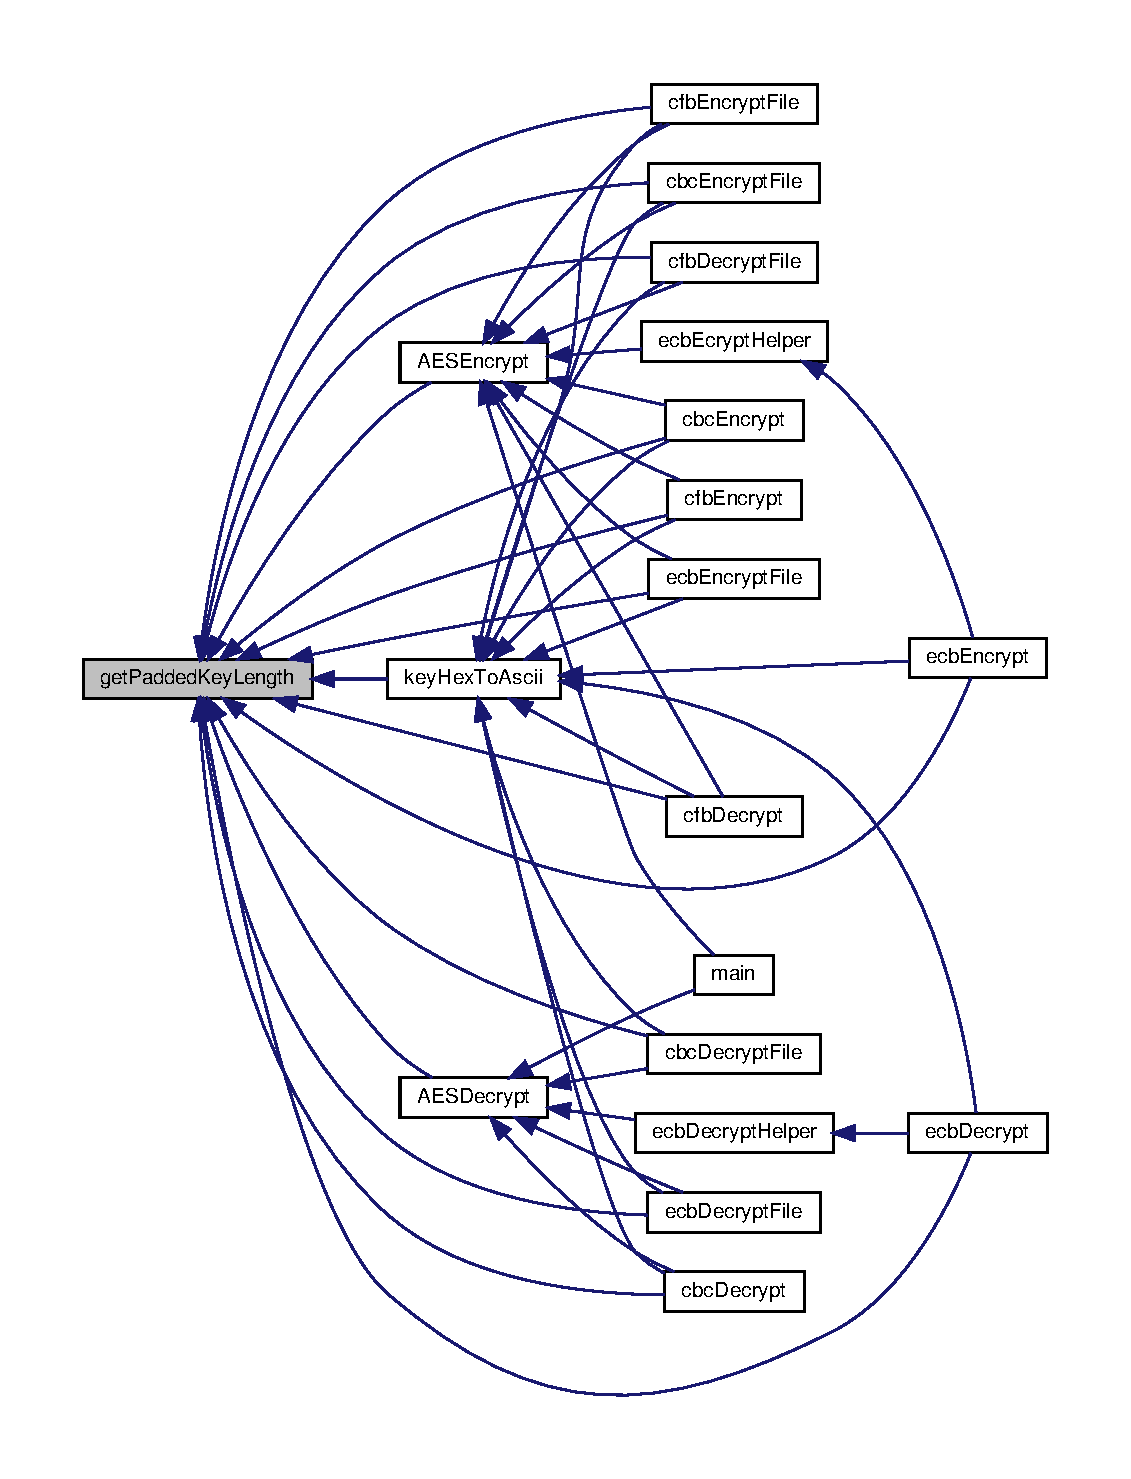
\includegraphics[width=350pt]{_a_e_s_8c_a5d65eac115e562c64b00a43e72ee6aca_icgraph}
\end{center}
\end{figure}
\mbox{\Hypertarget{_a_e_s_8c_a4e58d2e928429bc56387394251b8ece5}\label{_a_e_s_8c_a4e58d2e928429bc56387394251b8ece5}} 
\index{A\+E\+S.\+c@{A\+E\+S.\+c}!get\+Rcon\+Value@{get\+Rcon\+Value}}
\index{get\+Rcon\+Value@{get\+Rcon\+Value}!A\+E\+S.\+c@{A\+E\+S.\+c}}
\subsubsection{\texorpdfstring{get\+Rcon\+Value()}{getRconValue()}}
{\footnotesize\ttfamily unsigned char get\+Rcon\+Value (\begin{DoxyParamCaption}\item[{unsigned char}]{num }\end{DoxyParamCaption})}



get\+Rcon\+Value -\/ Function to return the Rcon value for the index passed in as a parameter 


\begin{DoxyParams}{Parameters}
{\em num.} & Requires the original value required in hex.\\
\hline
{\em index} & -\/ unsigned char -\/ hexadecimal representation of the number for which the Rcon value is required during the key schedule. \\
\hline
\end{DoxyParams}
\begin{DoxyReturn}{Returns}
unsigned char -\/ r\+Con value for the paramter 
\end{DoxyReturn}

\begin{DoxyParams}{Parameters}
{\em num.} & \\
\hline
\end{DoxyParams}


Definition at line 158 of file A\+E\+S.\+c.

Here is the caller graph for this function\+:\nopagebreak
\begin{figure}[H]
\begin{center}
\leavevmode
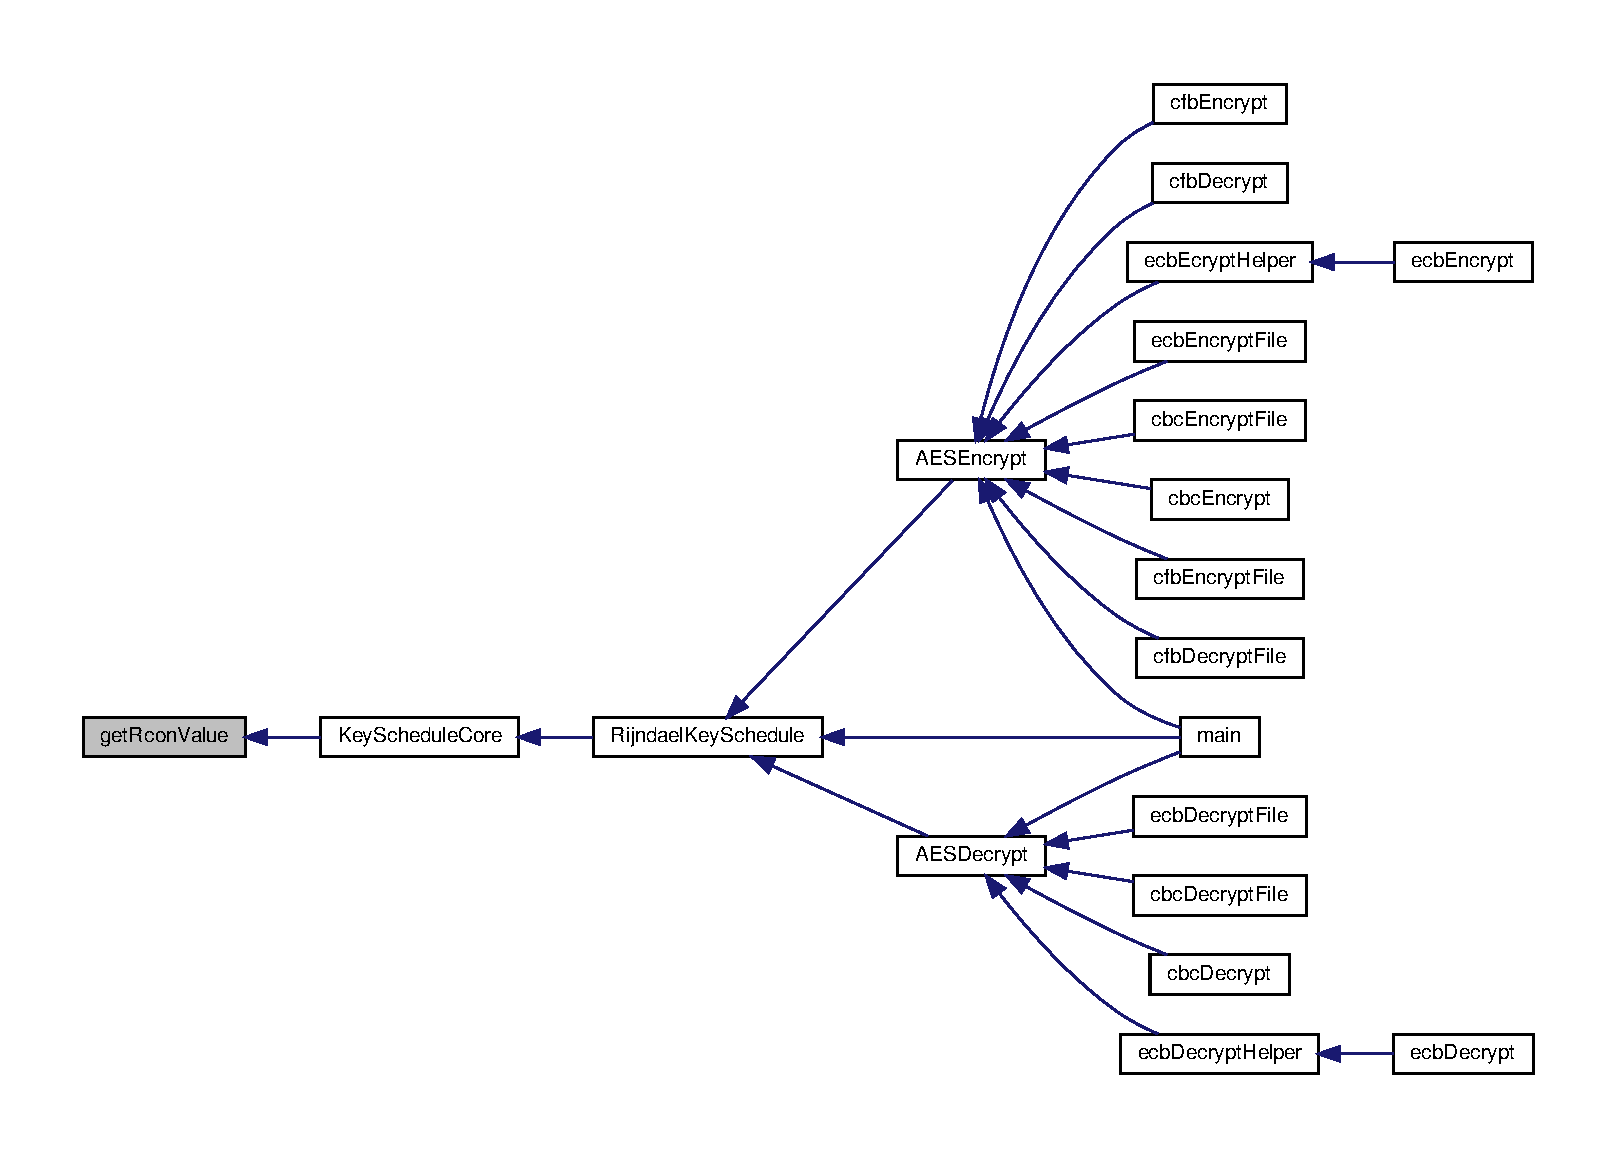
\includegraphics[width=350pt]{_a_e_s_8c_a4e58d2e928429bc56387394251b8ece5_icgraph}
\end{center}
\end{figure}
\mbox{\Hypertarget{_a_e_s_8c_abe15a731f43315f6f595674d3cd62d57}\label{_a_e_s_8c_abe15a731f43315f6f595674d3cd62d57}} 
\index{A\+E\+S.\+c@{A\+E\+S.\+c}!get\+Round\+Key@{get\+Round\+Key}}
\index{get\+Round\+Key@{get\+Round\+Key}!A\+E\+S.\+c@{A\+E\+S.\+c}}
\subsubsection{\texorpdfstring{get\+Round\+Key()}{getRoundKey()}}
{\footnotesize\ttfamily void get\+Round\+Key (\begin{DoxyParamCaption}\item[{unsigned char $\ast$}]{expanded\+Key,  }\item[{unsigned char $\ast$}]{round\+Key,  }\item[{int}]{round\+Num }\end{DoxyParamCaption})}



get\+Round\+Key -\/ Function to extract the correct sub-\/key to use for the appropriate round specified by 


\begin{DoxyParams}{Parameters}
{\em round\+Num.} & Copies the sub-\/key from the expanded key in \\
\hline
{\em expanded\+Key} & to \\
\hline
{\em round\+Key.} & \\
\hline
{\em char} & -\/ expanded\+Key -\/ The expanded key from which to extract the sub-\/key. \\
\hline
{\em char} & -\/ round\+Key -\/ memory to which to copy the sub-\/key. \\
\hline
{\em round\+Num} & -\/ int -\/ the round number for which the sub-\/key is required. \\
\hline
\end{DoxyParams}


Definition at line 881 of file A\+E\+S.\+c.

Here is the caller graph for this function\+:\nopagebreak
\begin{figure}[H]
\begin{center}
\leavevmode
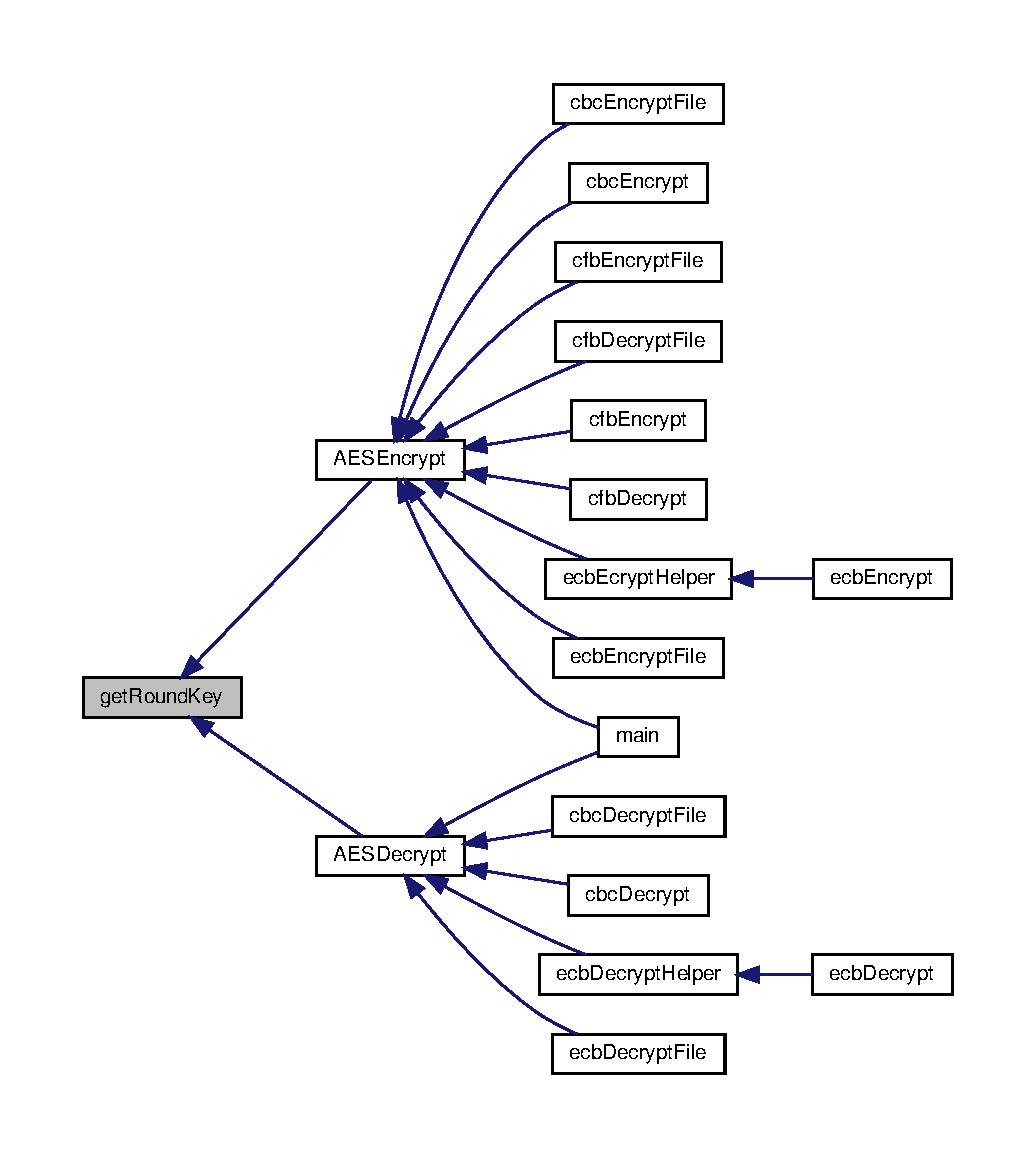
\includegraphics[width=350pt]{_a_e_s_8c_abe15a731f43315f6f595674d3cd62d57_icgraph}
\end{center}
\end{figure}
\mbox{\Hypertarget{_a_e_s_8c_acdf4abe2846c02b4d3e674782807fdfa}\label{_a_e_s_8c_acdf4abe2846c02b4d3e674782807fdfa}} 
\index{A\+E\+S.\+c@{A\+E\+S.\+c}!get\+S\+Box\+Value@{get\+S\+Box\+Value}}
\index{get\+S\+Box\+Value@{get\+S\+Box\+Value}!A\+E\+S.\+c@{A\+E\+S.\+c}}
\subsubsection{\texorpdfstring{get\+S\+Box\+Value()}{getSBoxValue()}}
{\footnotesize\ttfamily unsigned char get\+S\+Box\+Value (\begin{DoxyParamCaption}\item[{unsigned char}]{index }\end{DoxyParamCaption})}



get\+S\+Box\+Value -\/ Function to return the s\+Box value passed in as a parameter 


\begin{DoxyParams}{Parameters}
{\em index.} & Requires the original value required in hex.\\
\hline
{\em index} & -\/ unsigned char -\/ hexadecimal representation of the index for which the S\+Box value is required. \\
\hline
\end{DoxyParams}
\begin{DoxyReturn}{Returns}
unsigned char -\/ s\+Box value for the paramter 
\end{DoxyReturn}

\begin{DoxyParams}{Parameters}
{\em index.} & \\
\hline
\end{DoxyParams}


Definition at line 134 of file A\+E\+S.\+c.

Here is the caller graph for this function\+:\nopagebreak
\begin{figure}[H]
\begin{center}
\leavevmode
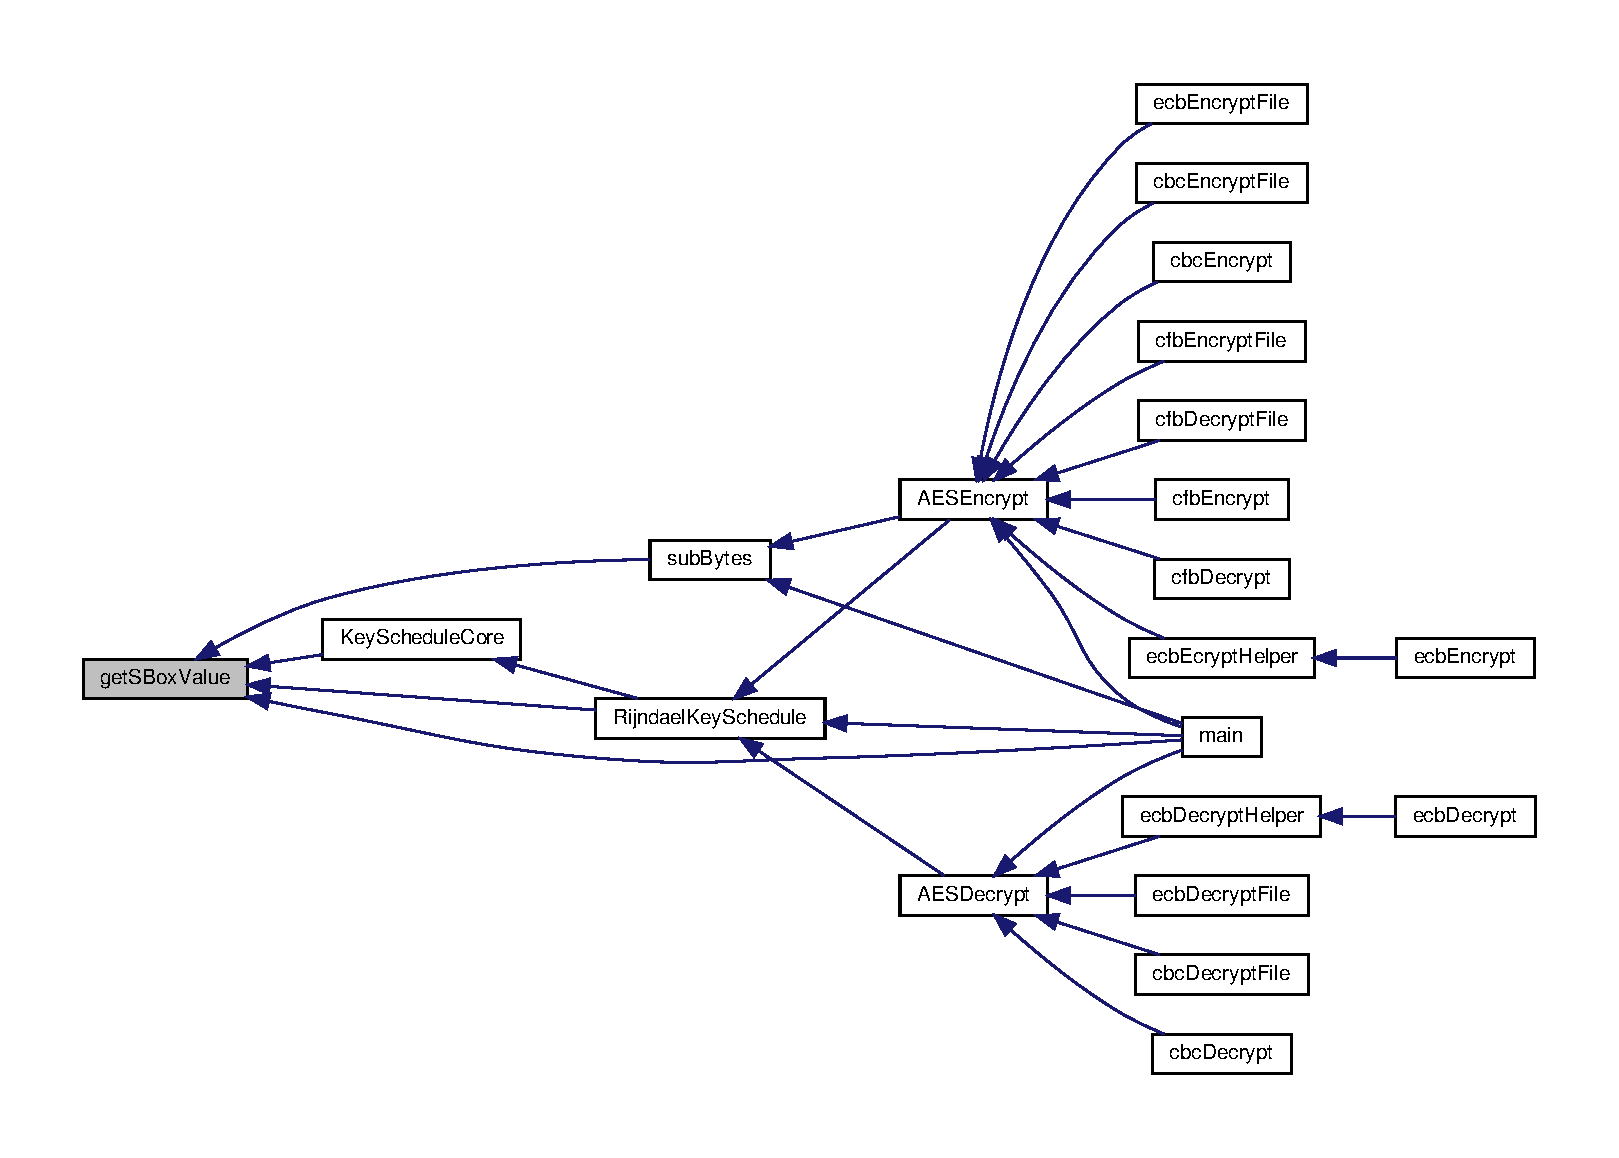
\includegraphics[width=350pt]{_a_e_s_8c_acdf4abe2846c02b4d3e674782807fdfa_icgraph}
\end{center}
\end{figure}
\mbox{\Hypertarget{_a_e_s_8c_aa177516503b10de65b504a3714073ad7}\label{_a_e_s_8c_aa177516503b10de65b504a3714073ad7}} 
\index{A\+E\+S.\+c@{A\+E\+S.\+c}!hex\+To\+Ascii@{hex\+To\+Ascii}}
\index{hex\+To\+Ascii@{hex\+To\+Ascii}!A\+E\+S.\+c@{A\+E\+S.\+c}}
\subsubsection{\texorpdfstring{hex\+To\+Ascii()}{hexToAscii()}}
{\footnotesize\ttfamily uint8\+\_\+t hex\+To\+Ascii (\begin{DoxyParamCaption}\item[{char}]{ch1,  }\item[{char}]{ch2 }\end{DoxyParamCaption})}



hex\+To\+Ascii -\/ Function that converts a given hex value to its A\+S\+C\+II equivalent. 


\begin{DoxyParams}{Parameters}
{\em ch1} & -\/ char value of the first hex value. \\
\hline
{\em ch2} & -\/ char value of the second hex value. \\
\hline
\end{DoxyParams}


Definition at line 928 of file A\+E\+S.\+c.

Here is the call graph for this function\+:\nopagebreak
\begin{figure}[H]
\begin{center}
\leavevmode
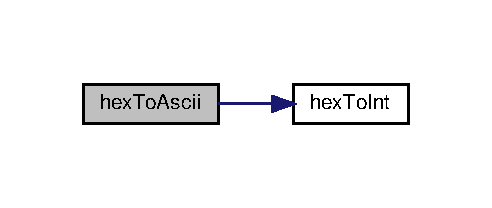
\includegraphics[width=236pt]{_a_e_s_8c_aa177516503b10de65b504a3714073ad7_cgraph}
\end{center}
\end{figure}
Here is the caller graph for this function\+:\nopagebreak
\begin{figure}[H]
\begin{center}
\leavevmode
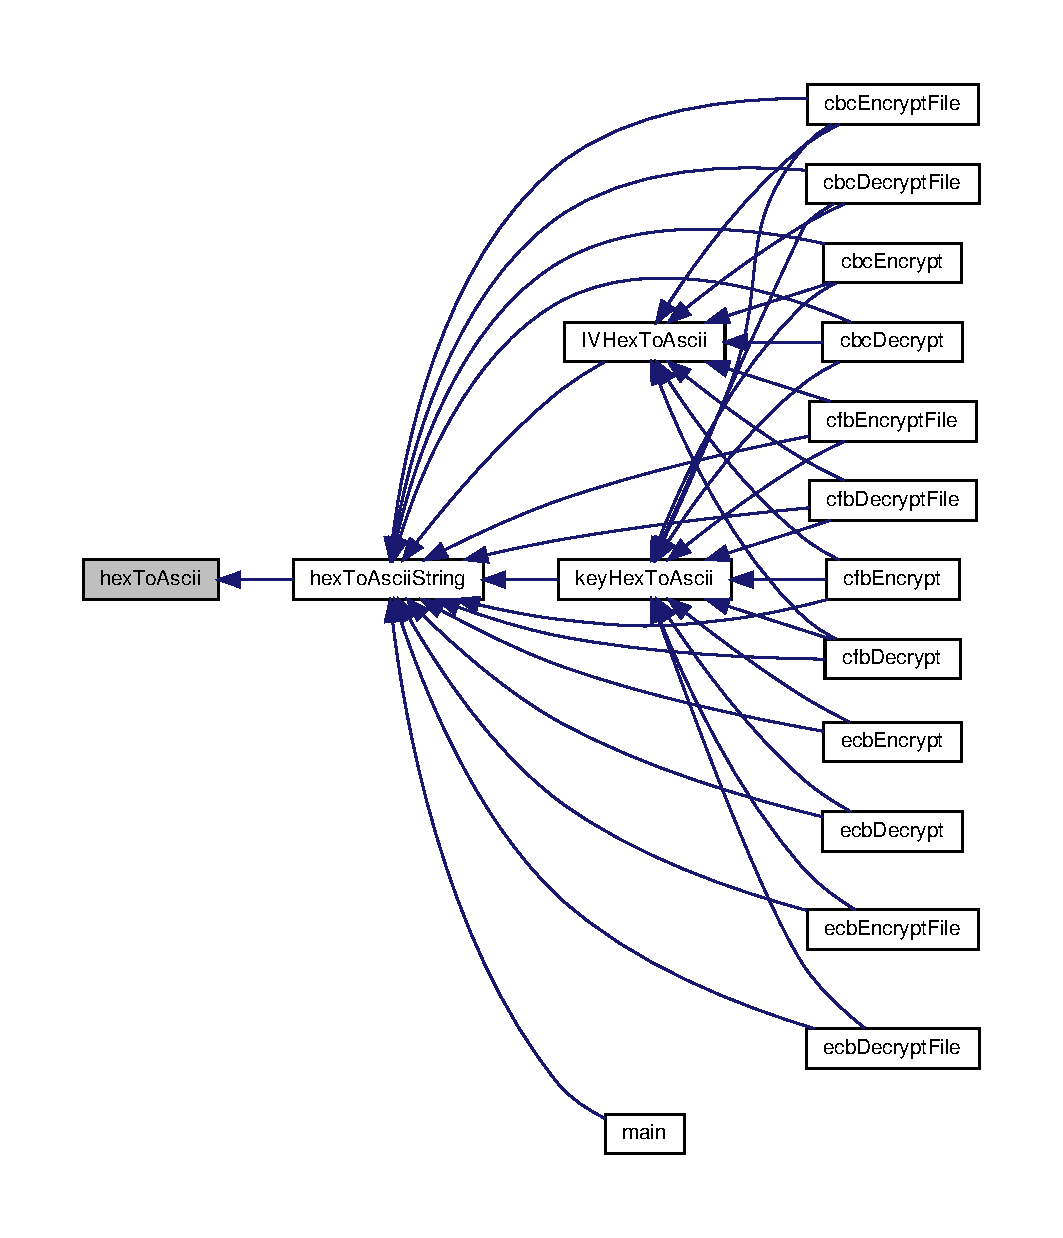
\includegraphics[width=350pt]{_a_e_s_8c_aa177516503b10de65b504a3714073ad7_icgraph}
\end{center}
\end{figure}
\mbox{\Hypertarget{_a_e_s_8c_ad697cbb5d9e462b3017df1f1d939ee96}\label{_a_e_s_8c_ad697cbb5d9e462b3017df1f1d939ee96}} 
\index{A\+E\+S.\+c@{A\+E\+S.\+c}!hex\+To\+Ascii\+String@{hex\+To\+Ascii\+String}}
\index{hex\+To\+Ascii\+String@{hex\+To\+Ascii\+String}!A\+E\+S.\+c@{A\+E\+S.\+c}}
\subsubsection{\texorpdfstring{hex\+To\+Ascii\+String()}{hexToAsciiString()}}
{\footnotesize\ttfamily void hex\+To\+Ascii\+String (\begin{DoxyParamCaption}\item[{char $\ast$}]{hex\+String,  }\item[{char $\ast$}]{ascii\+String,  }\item[{int}]{hex\+String\+Length }\end{DoxyParamCaption})}



hex\+To\+Ascii\+String -\/ Function that converts a given string of hex values into its A\+S\+C\+II equivalent. A hex string contains hex chars and is \char`\"{}encoded\char`\"{} in ascii In order to encrypt it, it must be converted to the equivalent ascii plain text string plaintext string is half the size of hex, since two hex chars = 1 ascii char if hex string is \char`\"{}4\+A\char`\"{} it will be converted to \char`\"{}\+J\char`\"{} in ascii which will have a hex representation of \char`\"{}4a\char`\"{} The original hex string converted to hex staright or printed in hex straight rather will print or have the value \char`\"{}0x34\char`\"{}, \char`\"{}0x31\char`\"{} B\+A\+S\+I\+C\+A\+L\+LY T\+HE H\+EX S\+T\+R\+I\+NG FF IS I\+N\+T\+E\+R\+P\+R\+E\+T\+ED AS T\+HE C\+H\+A\+RS FF, whereas when using this function we intend it to be \char`\"{}\+J\char`\"{}, ie the char \char`\"{}\+J\char`\"{} 


\begin{DoxyParams}{Parameters}
{\em char$\ast$} & hex\+String -\/ The string of hex values to be converted. \\
\hline
{\em char$\ast$} & ascii\+String -\/ The output of the converted hex string. \\
\hline
{\em int} & hex\+String\+Length -\/ The length of parameter hex\+String. \\
\hline
\end{DoxyParams}


Definition at line 948 of file A\+E\+S.\+c.

Here is the call graph for this function\+:\nopagebreak
\begin{figure}[H]
\begin{center}
\leavevmode
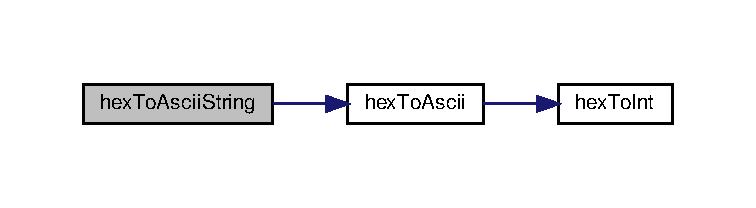
\includegraphics[width=350pt]{_a_e_s_8c_ad697cbb5d9e462b3017df1f1d939ee96_cgraph}
\end{center}
\end{figure}
Here is the caller graph for this function\+:\nopagebreak
\begin{figure}[H]
\begin{center}
\leavevmode
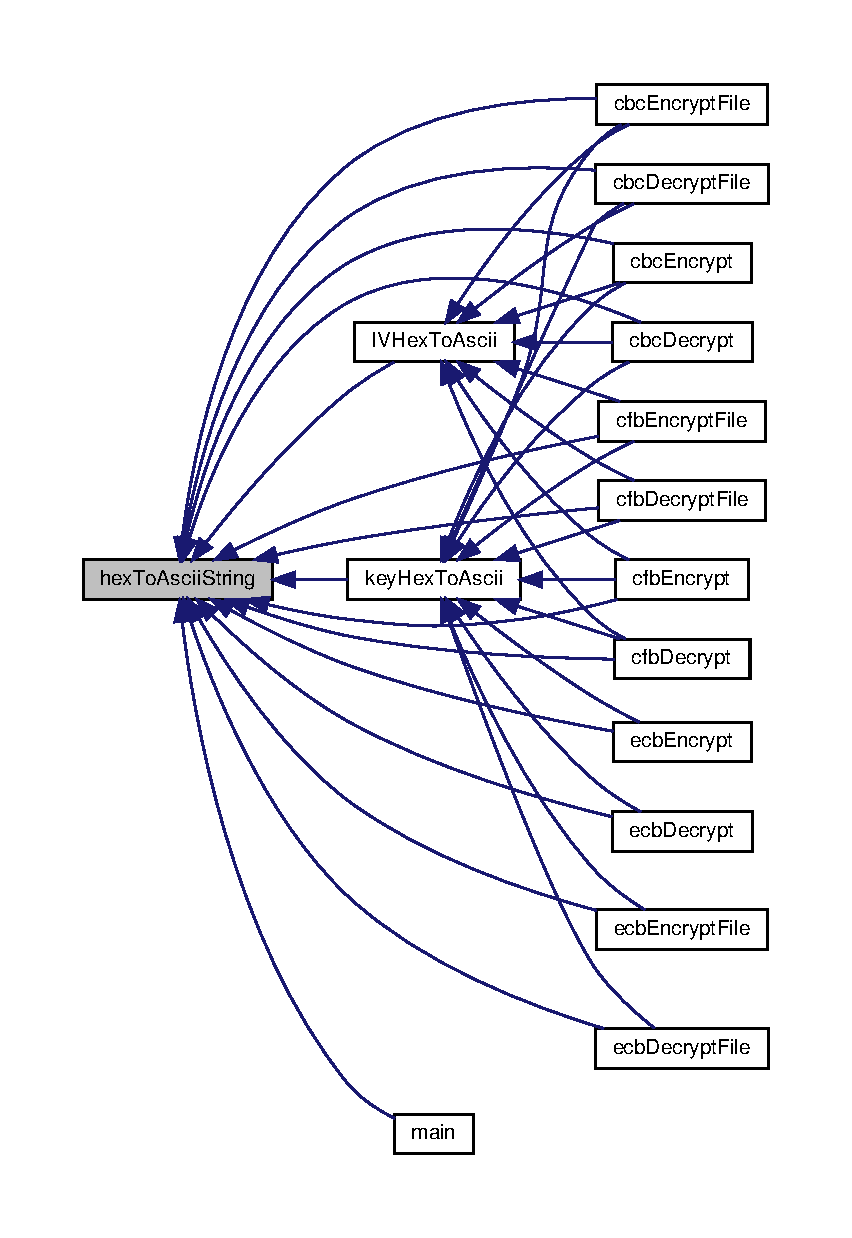
\includegraphics[width=350pt]{_a_e_s_8c_ad697cbb5d9e462b3017df1f1d939ee96_icgraph}
\end{center}
\end{figure}
\mbox{\Hypertarget{_a_e_s_8c_a7e5ab2188af44718071074f450963568}\label{_a_e_s_8c_a7e5ab2188af44718071074f450963568}} 
\index{A\+E\+S.\+c@{A\+E\+S.\+c}!hex\+To\+Int@{hex\+To\+Int}}
\index{hex\+To\+Int@{hex\+To\+Int}!A\+E\+S.\+c@{A\+E\+S.\+c}}
\subsubsection{\texorpdfstring{hex\+To\+Int()}{hexToInt()}}
{\footnotesize\ttfamily uint8\+\_\+t hex\+To\+Int (\begin{DoxyParamCaption}\item[{char}]{ch }\end{DoxyParamCaption})}



hex\+To\+Int -\/ Function that converts a given hex value into an integer. 


\begin{DoxyParams}{Parameters}
{\em ch} & -\/ hex value that wil be converted to int. \\
\hline
\end{DoxyParams}
\begin{DoxyReturn}{Returns}
uint8\+\_\+t the converted int value. 
\end{DoxyReturn}


Definition at line 909 of file A\+E\+S.\+c.

Here is the caller graph for this function\+:\nopagebreak
\begin{figure}[H]
\begin{center}
\leavevmode
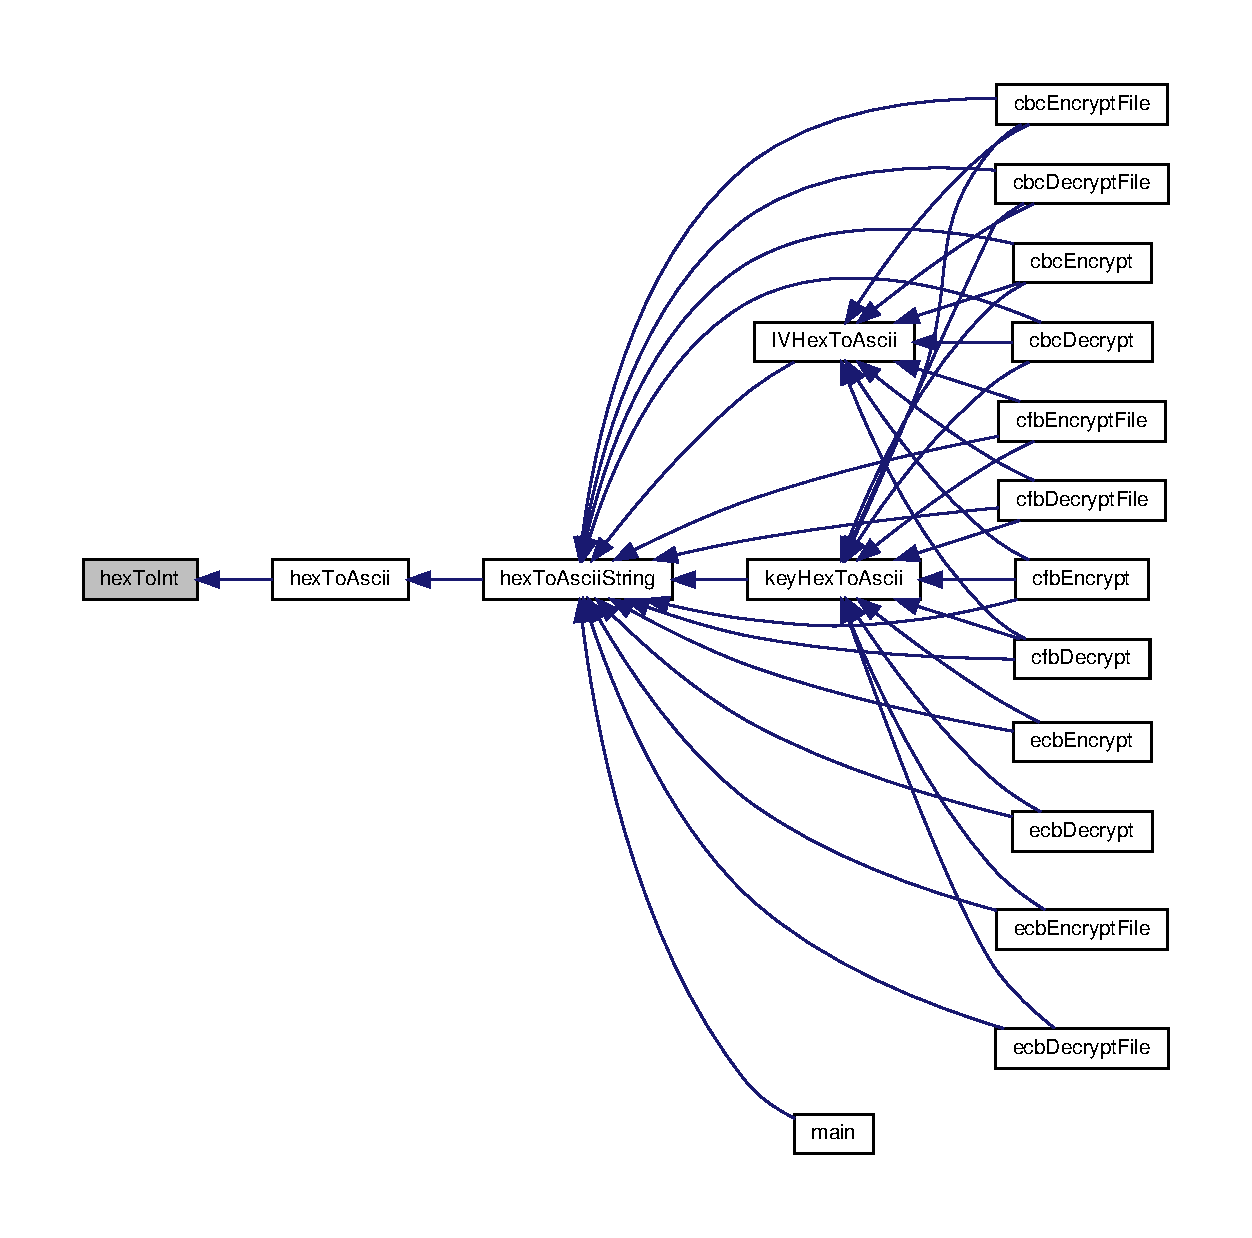
\includegraphics[width=350pt]{_a_e_s_8c_a7e5ab2188af44718071074f450963568_icgraph}
\end{center}
\end{figure}
\mbox{\Hypertarget{_a_e_s_8c_a9de891875f23dd3dff8fe3f8e10ba3ad}\label{_a_e_s_8c_a9de891875f23dd3dff8fe3f8e10ba3ad}} 
\index{A\+E\+S.\+c@{A\+E\+S.\+c}!inv\+Mix\+Columns@{inv\+Mix\+Columns}}
\index{inv\+Mix\+Columns@{inv\+Mix\+Columns}!A\+E\+S.\+c@{A\+E\+S.\+c}}
\subsubsection{\texorpdfstring{inv\+Mix\+Columns()}{invMixColumns()}}
{\footnotesize\ttfamily void inv\+Mix\+Columns (\begin{DoxyParamCaption}\item[{unsigned char}]{state\mbox{[}4\mbox{]}\mbox{[}4\mbox{]} }\end{DoxyParamCaption})}



inv\+Mix\+Columns -\/ Function that does the inverse of the Mix Column Step for A\+ES Encryption. Performs the gallois field multiplication and the required X\+OR to the state passed in as a paramter 


\begin{DoxyParams}{Parameters}
{\em state.} & \\
\hline
{\em state} & -\/ unsigned char -\/ is the current state of the ciphertext or plaintext during A\+ES encryption or decryption. \\
\hline
\end{DoxyParams}


Definition at line 740 of file A\+E\+S.\+c.

Here is the call graph for this function\+:\nopagebreak
\begin{figure}[H]
\begin{center}
\leavevmode
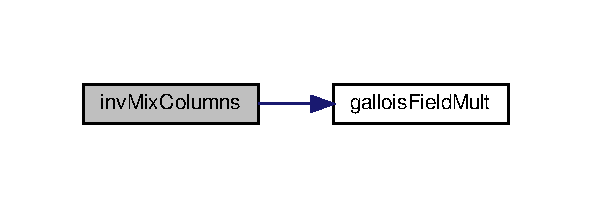
\includegraphics[width=284pt]{_a_e_s_8c_a9de891875f23dd3dff8fe3f8e10ba3ad_cgraph}
\end{center}
\end{figure}
Here is the caller graph for this function\+:\nopagebreak
\begin{figure}[H]
\begin{center}
\leavevmode
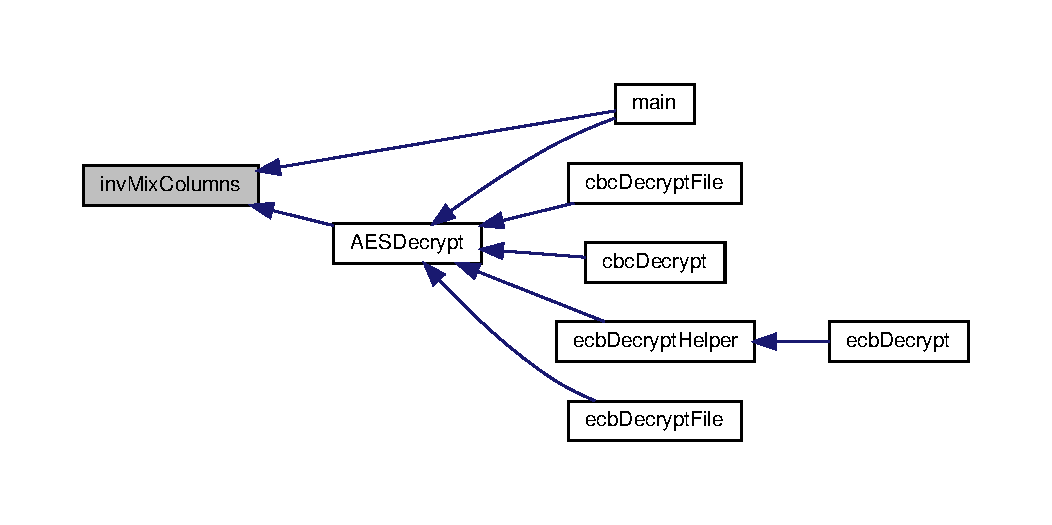
\includegraphics[width=350pt]{_a_e_s_8c_a9de891875f23dd3dff8fe3f8e10ba3ad_icgraph}
\end{center}
\end{figure}
\mbox{\Hypertarget{_a_e_s_8c_a903e34d08dd07be2e2d9618d4d489ee6}\label{_a_e_s_8c_a903e34d08dd07be2e2d9618d4d489ee6}} 
\index{A\+E\+S.\+c@{A\+E\+S.\+c}!inv\+Shift\+Rows@{inv\+Shift\+Rows}}
\index{inv\+Shift\+Rows@{inv\+Shift\+Rows}!A\+E\+S.\+c@{A\+E\+S.\+c}}
\subsubsection{\texorpdfstring{inv\+Shift\+Rows()}{invShiftRows()}}
{\footnotesize\ttfamily void inv\+Shift\+Rows (\begin{DoxyParamCaption}\item[{unsigned char}]{state\mbox{[}4\mbox{]}\mbox{[}4\mbox{]},  }\item[{int}]{word\+Length }\end{DoxyParamCaption})}



inv\+Shift\+Rows -\/ Function to shift the state array Inverse according to the A\+ES encryption standard for 128 -\/ bits blocks 


\begin{DoxyParams}{Parameters}
{\em state} & -\/ unsigned char -\/ is the current state of the ciphertext or plaintext during A\+ES encryption or decryption \\
\hline
\end{DoxyParams}


Definition at line 835 of file A\+E\+S.\+c.

Here is the call graph for this function\+:\nopagebreak
\begin{figure}[H]
\begin{center}
\leavevmode
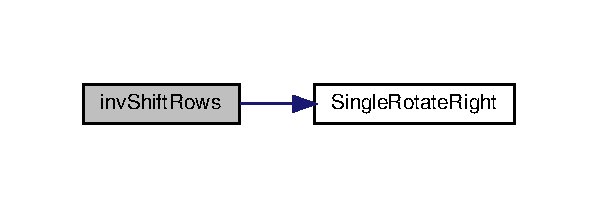
\includegraphics[width=287pt]{_a_e_s_8c_a903e34d08dd07be2e2d9618d4d489ee6_cgraph}
\end{center}
\end{figure}
Here is the caller graph for this function\+:\nopagebreak
\begin{figure}[H]
\begin{center}
\leavevmode
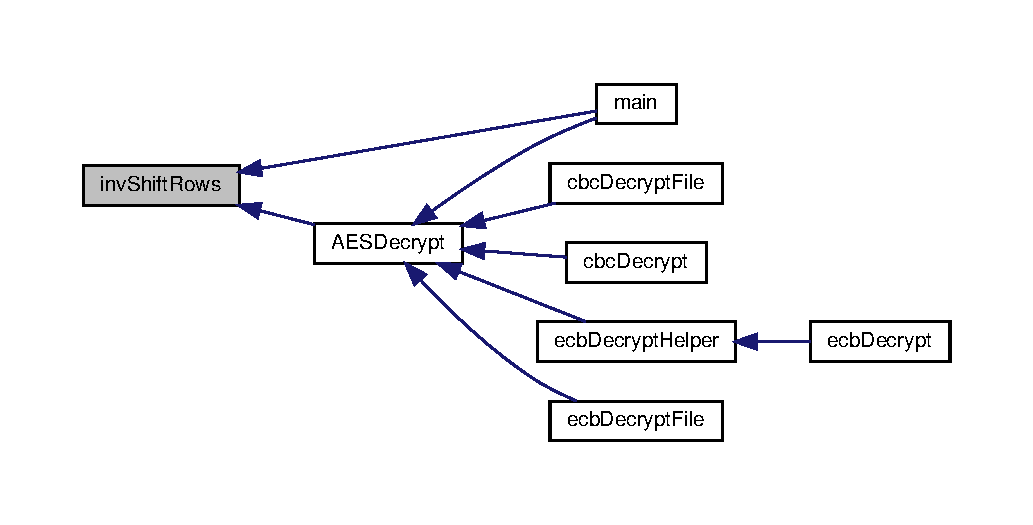
\includegraphics[width=350pt]{_a_e_s_8c_a903e34d08dd07be2e2d9618d4d489ee6_icgraph}
\end{center}
\end{figure}
\mbox{\Hypertarget{_a_e_s_8c_a8e72edc1f652f8626aacd2781303c86b}\label{_a_e_s_8c_a8e72edc1f652f8626aacd2781303c86b}} 
\index{A\+E\+S.\+c@{A\+E\+S.\+c}!inv\+Sub\+Bytes@{inv\+Sub\+Bytes}}
\index{inv\+Sub\+Bytes@{inv\+Sub\+Bytes}!A\+E\+S.\+c@{A\+E\+S.\+c}}
\subsubsection{\texorpdfstring{inv\+Sub\+Bytes()}{invSubBytes()}}
{\footnotesize\ttfamily void inv\+Sub\+Bytes (\begin{DoxyParamCaption}\item[{unsigned char}]{state\mbox{[}4\mbox{]}\mbox{[}4\mbox{]} }\end{DoxyParamCaption})}



inv\+Sub\+Bytes -\/ Function that performs the inverse of Function sub\+Bytes 


\begin{DoxyParams}{Parameters}
{\em state} & -\/ unsigned char -\/ is the current state of the ciphertext or plaintext during A\+ES encryption or decryption \\
\hline
\end{DoxyParams}


Definition at line 802 of file A\+E\+S.\+c.

Here is the call graph for this function\+:\nopagebreak
\begin{figure}[H]
\begin{center}
\leavevmode
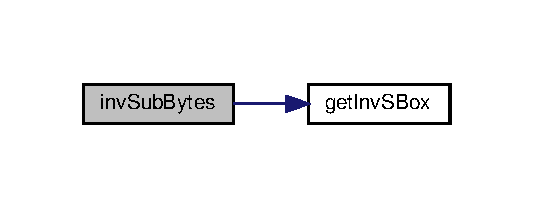
\includegraphics[width=256pt]{_a_e_s_8c_a8e72edc1f652f8626aacd2781303c86b_cgraph}
\end{center}
\end{figure}
Here is the caller graph for this function\+:\nopagebreak
\begin{figure}[H]
\begin{center}
\leavevmode
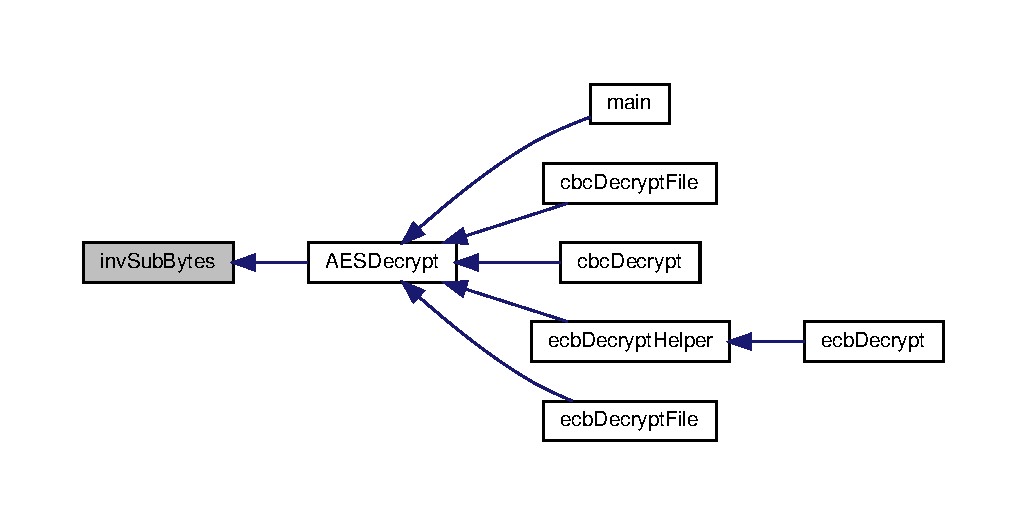
\includegraphics[width=350pt]{_a_e_s_8c_a8e72edc1f652f8626aacd2781303c86b_icgraph}
\end{center}
\end{figure}
\mbox{\Hypertarget{_a_e_s_8c_a3bf513612c15693c3b2be10b94298e05}\label{_a_e_s_8c_a3bf513612c15693c3b2be10b94298e05}} 
\index{A\+E\+S.\+c@{A\+E\+S.\+c}!is\+File\+Txt@{is\+File\+Txt}}
\index{is\+File\+Txt@{is\+File\+Txt}!A\+E\+S.\+c@{A\+E\+S.\+c}}
\subsubsection{\texorpdfstring{is\+File\+Txt()}{isFileTxt()}}
{\footnotesize\ttfamily uint8\+\_\+t is\+File\+Txt (\begin{DoxyParamCaption}\item[{unsigned char $\ast$}]{file\+Name }\end{DoxyParamCaption})}



is\+File\+Txt -\/ Function to determine if the file passed in as a paramter 


\begin{DoxyParams}{Parameters}
{\em filename} & is a text file with extension .txt or not. Returns a 1 if it is and a 0 if it isn\textquotesingle{}t.\\
\hline
{\em file\+Name} & -\/ unsigned char$\ast$ file\+Name -\/ path to file to determine if the file is a text file or not. \\
\hline
\end{DoxyParams}
\begin{DoxyReturn}{Returns}
uint8\+\_\+t -\/ boolean indicating if it is a text file or not. (0 is not a text file, 1 is a text file) 
\end{DoxyReturn}


Definition at line 1156 of file A\+E\+S.\+c.

Here is the caller graph for this function\+:\nopagebreak
\begin{figure}[H]
\begin{center}
\leavevmode
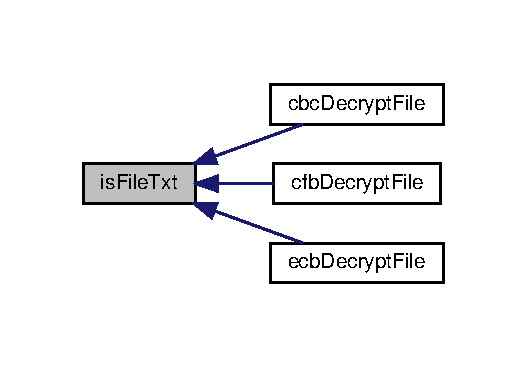
\includegraphics[width=253pt]{_a_e_s_8c_a3bf513612c15693c3b2be10b94298e05_icgraph}
\end{center}
\end{figure}
\mbox{\Hypertarget{_a_e_s_8c_ad82d1b77336ac1292ed5a24b92380f42}\label{_a_e_s_8c_ad82d1b77336ac1292ed5a24b92380f42}} 
\index{A\+E\+S.\+c@{A\+E\+S.\+c}!I\+V\+Hex\+To\+Ascii@{I\+V\+Hex\+To\+Ascii}}
\index{I\+V\+Hex\+To\+Ascii@{I\+V\+Hex\+To\+Ascii}!A\+E\+S.\+c@{A\+E\+S.\+c}}
\subsubsection{\texorpdfstring{I\+V\+Hex\+To\+Ascii()}{IVHexToAscii()}}
{\footnotesize\ttfamily unsigned char$\ast$ I\+V\+Hex\+To\+Ascii (\begin{DoxyParamCaption}\item[{unsigned char $\ast$}]{hex\+IV,  }\item[{int}]{I\+V\+Length }\end{DoxyParamCaption})}



I\+V\+Hex\+To\+Ascii -\/ Function to convert a initialization vector from a Hex string passed in as a paramter. 


\begin{DoxyParams}{Parameters}
{\em hex\+IV} & to an ascii string. User must free the returned pointer to memory allocated. Returns the Ascii equivalent. The caller must free the pointer returned. \\
\hline
{\em char} & -\/ unsigned char$\ast$ hex\+IV -\/ hex representation \\
\hline
{\em I\+V\+Length} & -\/ length of the hex representation of the IV passed in as paramter \\
\hline
{\em hex\+I\+V.} & \\
\hline
\end{DoxyParams}
\begin{DoxyReturn}{Returns}
unsigned$\ast$ -\/ the A\+S\+C\+II representation of the hex IV passed in as parameter 
\end{DoxyReturn}

\begin{DoxyParams}{Parameters}
{\em hex\+I\+V.} & \\
\hline
\end{DoxyParams}


Definition at line 1205 of file A\+E\+S.\+c.

Here is the call graph for this function\+:\nopagebreak
\begin{figure}[H]
\begin{center}
\leavevmode
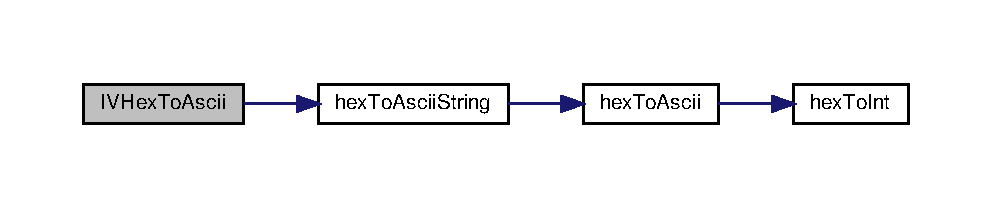
\includegraphics[width=350pt]{_a_e_s_8c_ad82d1b77336ac1292ed5a24b92380f42_cgraph}
\end{center}
\end{figure}
Here is the caller graph for this function\+:\nopagebreak
\begin{figure}[H]
\begin{center}
\leavevmode
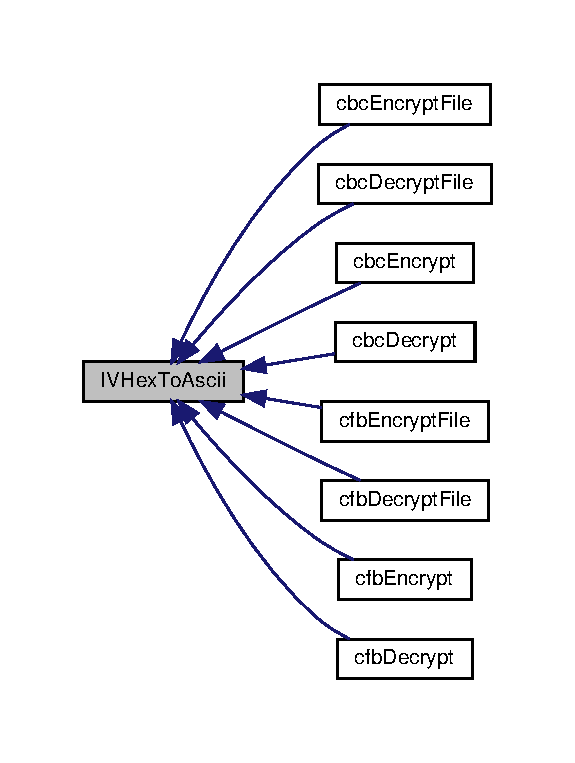
\includegraphics[width=276pt]{_a_e_s_8c_ad82d1b77336ac1292ed5a24b92380f42_icgraph}
\end{center}
\end{figure}
\mbox{\Hypertarget{_a_e_s_8c_afba897e91364663f883cc51ed309dc92}\label{_a_e_s_8c_afba897e91364663f883cc51ed309dc92}} 
\index{A\+E\+S.\+c@{A\+E\+S.\+c}!key\+Hex\+To\+Ascii@{key\+Hex\+To\+Ascii}}
\index{key\+Hex\+To\+Ascii@{key\+Hex\+To\+Ascii}!A\+E\+S.\+c@{A\+E\+S.\+c}}
\subsubsection{\texorpdfstring{key\+Hex\+To\+Ascii()}{keyHexToAscii()}}
{\footnotesize\ttfamily unsigned char$\ast$ key\+Hex\+To\+Ascii (\begin{DoxyParamCaption}\item[{unsigned char $\ast$}]{hex\+Key,  }\item[{int}]{key\+Length }\end{DoxyParamCaption})}



key\+Hex\+To\+Ascii -\/ Function to convert a key from a Hex string passed in as a paramter 


\begin{DoxyParams}{Parameters}
{\em hex\+Key} & to an ascii string. User must free the returned pointer to memory allocated. Returns the Ascii equivalent. The caller must free the pointer returned. \\
\hline
{\em char} & -\/ unsigned char$\ast$ hex\+Key -\/ hex representation of the key to be converted to A\+S\+C\+II. \\
\hline
{\em key\+Length} & -\/ length of the hex representation of the key passed in as paramter \\
\hline
{\em hex\+Key.} & \\
\hline
\end{DoxyParams}
\begin{DoxyReturn}{Returns}
unsigned$\ast$ -\/ the A\+S\+C\+II representation of the hex key passed in as parameter 
\end{DoxyReturn}

\begin{DoxyParams}{Parameters}
{\em hex\+Key.} & \\
\hline
\end{DoxyParams}


Definition at line 1178 of file A\+E\+S.\+c.

Here is the call graph for this function\+:\nopagebreak
\begin{figure}[H]
\begin{center}
\leavevmode
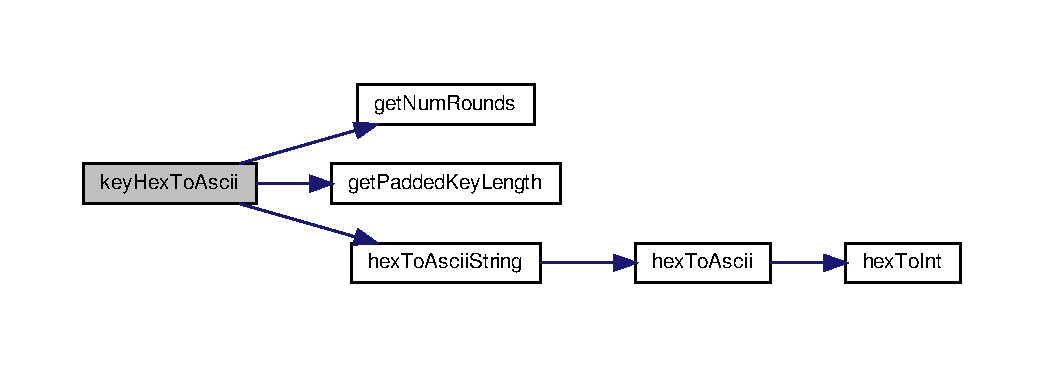
\includegraphics[width=350pt]{_a_e_s_8c_afba897e91364663f883cc51ed309dc92_cgraph}
\end{center}
\end{figure}
Here is the caller graph for this function\+:\nopagebreak
\begin{figure}[H]
\begin{center}
\leavevmode
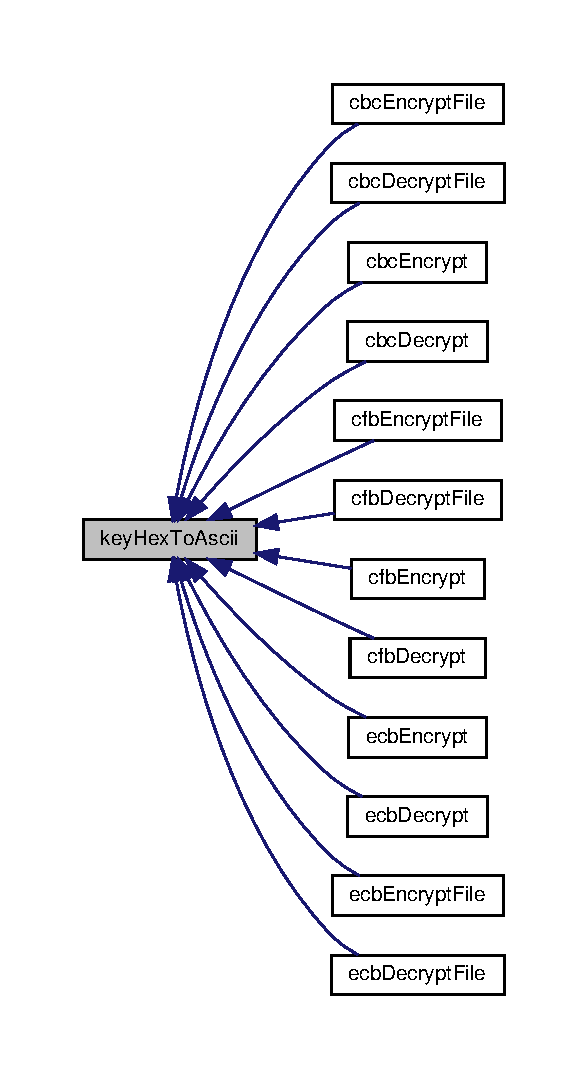
\includegraphics[width=282pt]{_a_e_s_8c_afba897e91364663f883cc51ed309dc92_icgraph}
\end{center}
\end{figure}
\mbox{\Hypertarget{_a_e_s_8c_af2f914cf17729a0ee89102c98b39665e}\label{_a_e_s_8c_af2f914cf17729a0ee89102c98b39665e}} 
\index{A\+E\+S.\+c@{A\+E\+S.\+c}!Key\+Schedule\+Core@{Key\+Schedule\+Core}}
\index{Key\+Schedule\+Core@{Key\+Schedule\+Core}!A\+E\+S.\+c@{A\+E\+S.\+c}}
\subsubsection{\texorpdfstring{Key\+Schedule\+Core()}{KeyScheduleCore()}}
{\footnotesize\ttfamily void Key\+Schedule\+Core (\begin{DoxyParamCaption}\item[{unsigned char $\ast$}]{word,  }\item[{int}]{word\+Length,  }\item[{int}]{r\+Con\+Iteration\+Val }\end{DoxyParamCaption})}



Key\+Schedule\+Core -\/ Function that performs the key schedule core for the Rijndael Key Schedule. Performs a single rotate left of the word passed in as. 


\begin{DoxyParams}{Parameters}
{\em word} & and applies the required s-\/box substituion and rcon X\+OR. \\
\hline
{\em char} & -\/ unsigned char$\ast$ word -\/ pointer to the word onto which the key schedule core should be operated. \\
\hline
{\em word\+Length} & -\/ length of the word passed in as a parameter \\
\hline
{\em word.} & \\
\hline
{\em r\+Con\+Iteration\+Val} & -\/ the iteration value to be used for the rcon X\+OR. \\
\hline
\end{DoxyParams}


Definition at line 631 of file A\+E\+S.\+c.

Here is the call graph for this function\+:\nopagebreak
\begin{figure}[H]
\begin{center}
\leavevmode
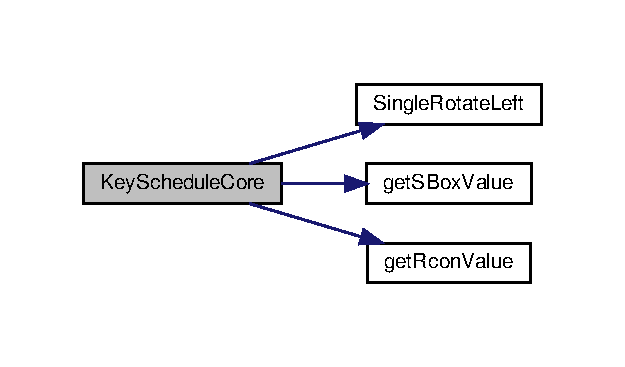
\includegraphics[width=300pt]{_a_e_s_8c_af2f914cf17729a0ee89102c98b39665e_cgraph}
\end{center}
\end{figure}
Here is the caller graph for this function\+:\nopagebreak
\begin{figure}[H]
\begin{center}
\leavevmode
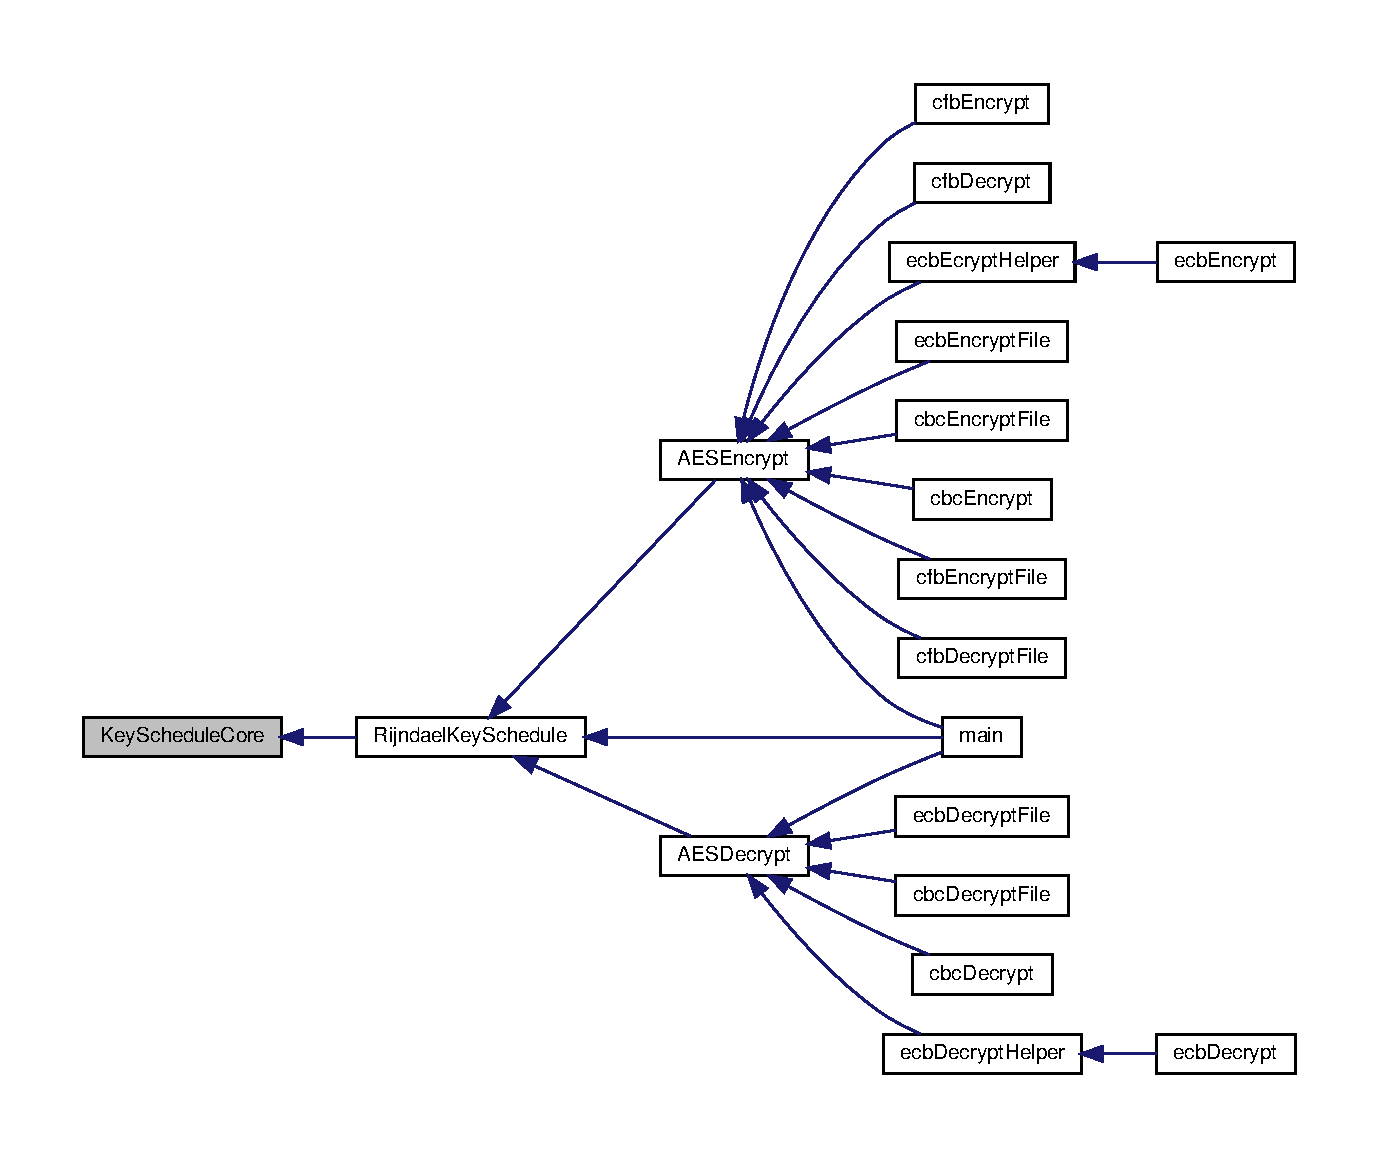
\includegraphics[width=350pt]{_a_e_s_8c_af2f914cf17729a0ee89102c98b39665e_icgraph}
\end{center}
\end{figure}
\mbox{\Hypertarget{_a_e_s_8c_aca09b30896a351db6587639a1cc1bf0d}\label{_a_e_s_8c_aca09b30896a351db6587639a1cc1bf0d}} 
\index{A\+E\+S.\+c@{A\+E\+S.\+c}!mix\+Columns@{mix\+Columns}}
\index{mix\+Columns@{mix\+Columns}!A\+E\+S.\+c@{A\+E\+S.\+c}}
\subsubsection{\texorpdfstring{mix\+Columns()}{mixColumns()}}
{\footnotesize\ttfamily void mix\+Columns (\begin{DoxyParamCaption}\item[{unsigned char}]{state\mbox{[}4\mbox{]}\mbox{[}4\mbox{]} }\end{DoxyParamCaption})}



mix\+Columns -\/ Function that performs the Mix\+Columns step of A\+ES as specified by A\+ES encryption. 


\begin{DoxyParams}{Parameters}
{\em state} & -\/ unsigned char -\/ is the current state of the ciphertext or plaintext during A\+ES encryption or decryption \\
\hline
\end{DoxyParams}


Definition at line 702 of file A\+E\+S.\+c.

Here is the caller graph for this function\+:\nopagebreak
\begin{figure}[H]
\begin{center}
\leavevmode
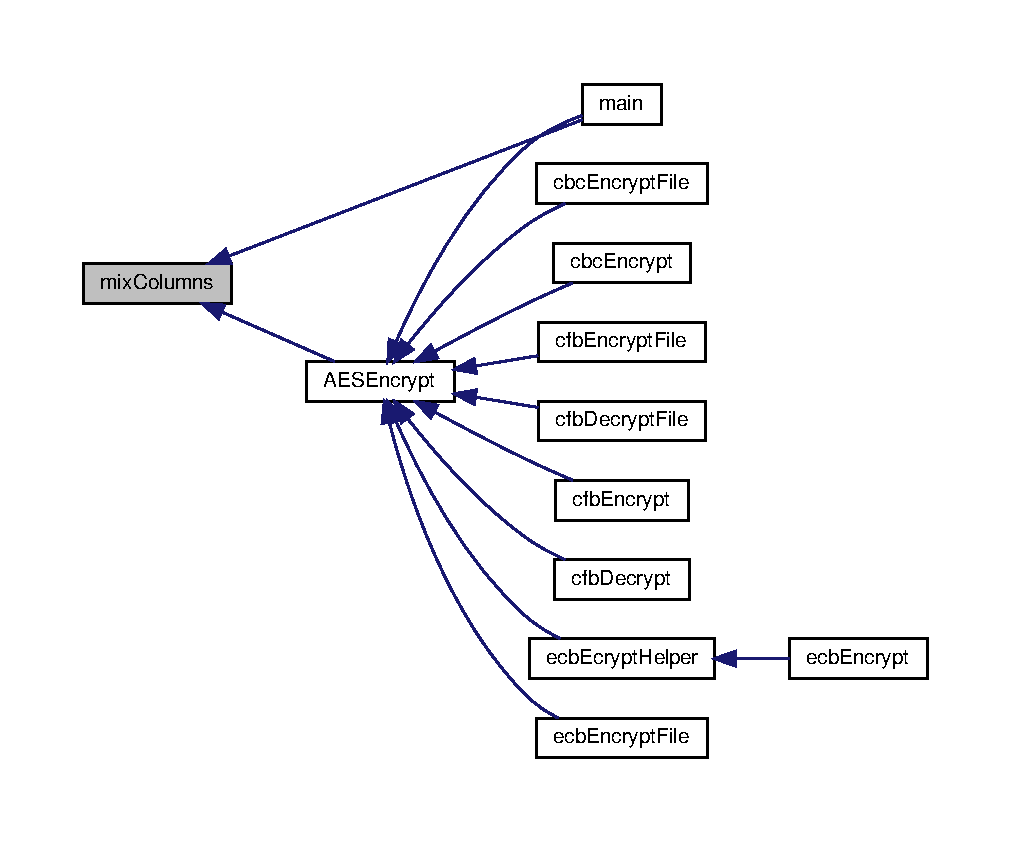
\includegraphics[width=350pt]{_a_e_s_8c_aca09b30896a351db6587639a1cc1bf0d_icgraph}
\end{center}
\end{figure}
\mbox{\Hypertarget{_a_e_s_8c_aaba2e1b9466483b3c6b8669eb42aa5ed}\label{_a_e_s_8c_aaba2e1b9466483b3c6b8669eb42aa5ed}} 
\index{A\+E\+S.\+c@{A\+E\+S.\+c}!print\+A\+E\+S\+Block@{print\+A\+E\+S\+Block}}
\index{print\+A\+E\+S\+Block@{print\+A\+E\+S\+Block}!A\+E\+S.\+c@{A\+E\+S.\+c}}
\subsubsection{\texorpdfstring{print\+A\+E\+S\+Block()}{printAESBlock()}}
{\footnotesize\ttfamily void print\+A\+E\+S\+Block (\begin{DoxyParamCaption}\item[{unsigned char $\ast$}]{block }\end{DoxyParamCaption})}



print\+A\+E\+S\+Block -\/ Function to print a single block in hex format to the terminal. 


\begin{DoxyParams}{Parameters}
{\em block} & -\/ block to be printed. \\
\hline
\end{DoxyParams}


Definition at line 1028 of file A\+E\+S.\+c.

Here is the caller graph for this function\+:\nopagebreak
\begin{figure}[H]
\begin{center}
\leavevmode
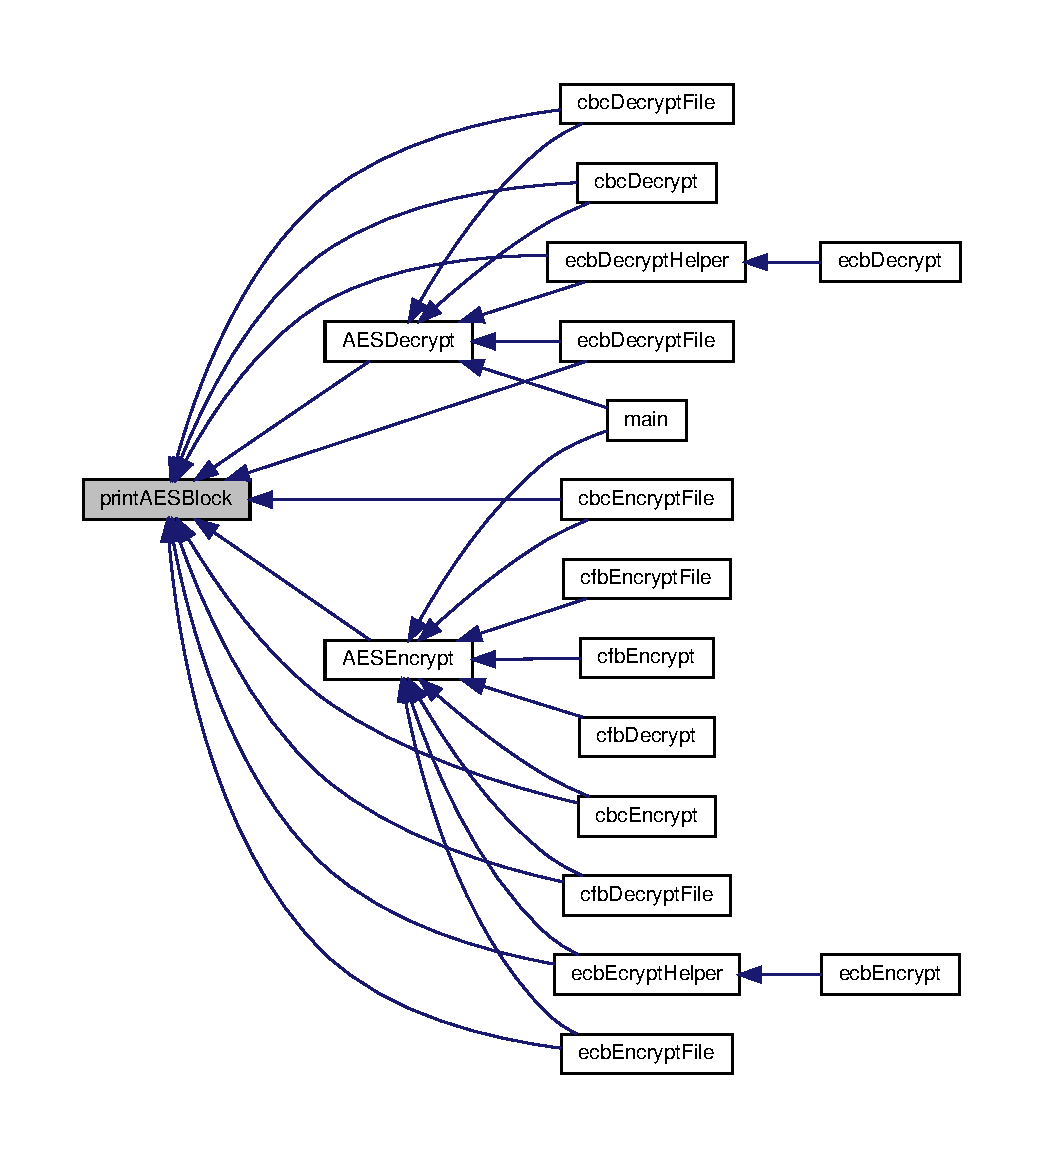
\includegraphics[width=350pt]{_a_e_s_8c_aaba2e1b9466483b3c6b8669eb42aa5ed_icgraph}
\end{center}
\end{figure}
\mbox{\Hypertarget{_a_e_s_8c_ae9af90db32afa65125a7eec339ed9d58}\label{_a_e_s_8c_ae9af90db32afa65125a7eec339ed9d58}} 
\index{A\+E\+S.\+c@{A\+E\+S.\+c}!print\+State\+Array@{print\+State\+Array}}
\index{print\+State\+Array@{print\+State\+Array}!A\+E\+S.\+c@{A\+E\+S.\+c}}
\subsubsection{\texorpdfstring{print\+State\+Array()}{printStateArray()}}
{\footnotesize\ttfamily void print\+State\+Array (\begin{DoxyParamCaption}\item[{uint8\+\_\+t}]{state\+Array\mbox{[}4\mbox{]}\mbox{[}4\mbox{]} }\end{DoxyParamCaption})}



print\+State\+Array -\/ Function to print the state array to the terminal in hex format. 


\begin{DoxyParams}{Parameters}
{\em state\+Array} & -\/ the state array that should be printed to the terminal. \\
\hline
\end{DoxyParams}


Definition at line 673 of file A\+E\+S.\+c.

Here is the caller graph for this function\+:\nopagebreak
\begin{figure}[H]
\begin{center}
\leavevmode
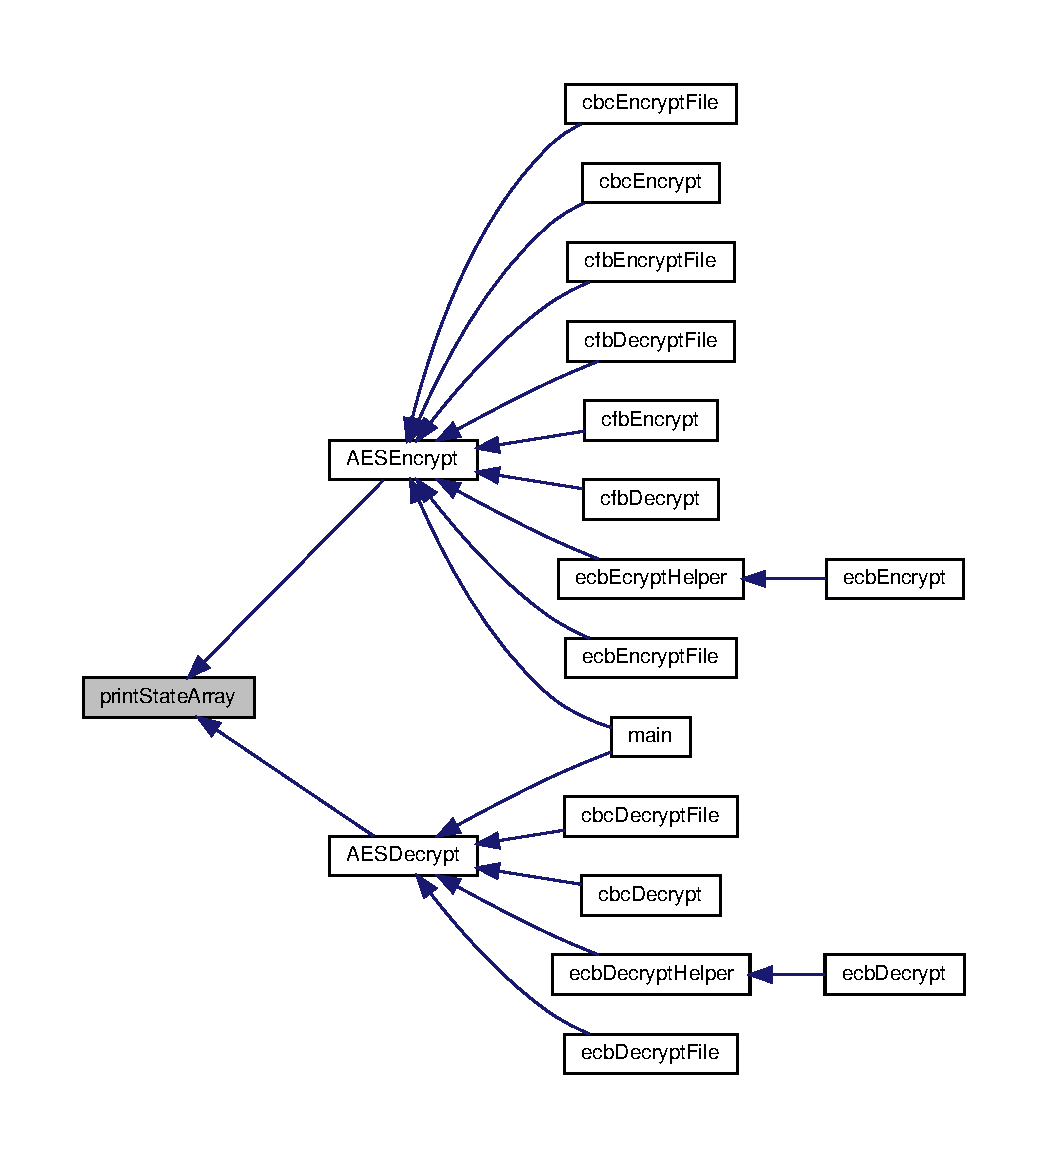
\includegraphics[width=350pt]{_a_e_s_8c_ae9af90db32afa65125a7eec339ed9d58_icgraph}
\end{center}
\end{figure}
\mbox{\Hypertarget{_a_e_s_8c_a185c827e4ccbc8e4608e83dfbf9dfc8e}\label{_a_e_s_8c_a185c827e4ccbc8e4608e83dfbf9dfc8e}} 
\index{A\+E\+S.\+c@{A\+E\+S.\+c}!Rijndael\+Key\+Schedule@{Rijndael\+Key\+Schedule}}
\index{Rijndael\+Key\+Schedule@{Rijndael\+Key\+Schedule}!A\+E\+S.\+c@{A\+E\+S.\+c}}
\subsubsection{\texorpdfstring{Rijndael\+Key\+Schedule()}{RijndaelKeySchedule()}}
{\footnotesize\ttfamily unsigned char$\ast$ Rijndael\+Key\+Schedule (\begin{DoxyParamCaption}\item[{unsigned char $\ast$}]{original\+Key,  }\item[{int}]{key\+Length }\end{DoxyParamCaption})}



Rijndael\+Key\+Schedule -\/ Function that performs the Rijndael key scheduling for A\+ES encryption. Takes in the original key passed in as parameter. 


\begin{DoxyParams}{Parameters}
{\em original\+Key} & and the length of the original key given as parameter. The caller must free the memory allocated and returned. \\
\hline
{\em original\+Key} & -\/ unsigned char $\ast$ -\/ An unsigned char pointer to the original key. \\
\hline
{\em key\+Length} & -\/ int -\/ length of original\+Key passed in as a parameter \\
\hline
{\em original\+Key} & \\
\hline
\end{DoxyParams}
\begin{DoxyReturn}{Returns}
expanded\+Key -\/ The key that has been expanded. 
\end{DoxyReturn}


Definition at line 577 of file A\+E\+S.\+c.

Here is the call graph for this function\+:\nopagebreak
\begin{figure}[H]
\begin{center}
\leavevmode
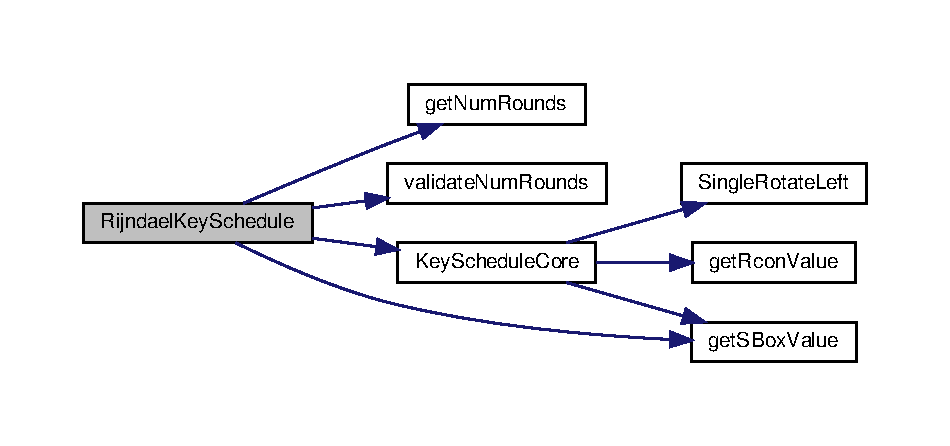
\includegraphics[width=350pt]{_a_e_s_8c_a185c827e4ccbc8e4608e83dfbf9dfc8e_cgraph}
\end{center}
\end{figure}
Here is the caller graph for this function\+:\nopagebreak
\begin{figure}[H]
\begin{center}
\leavevmode
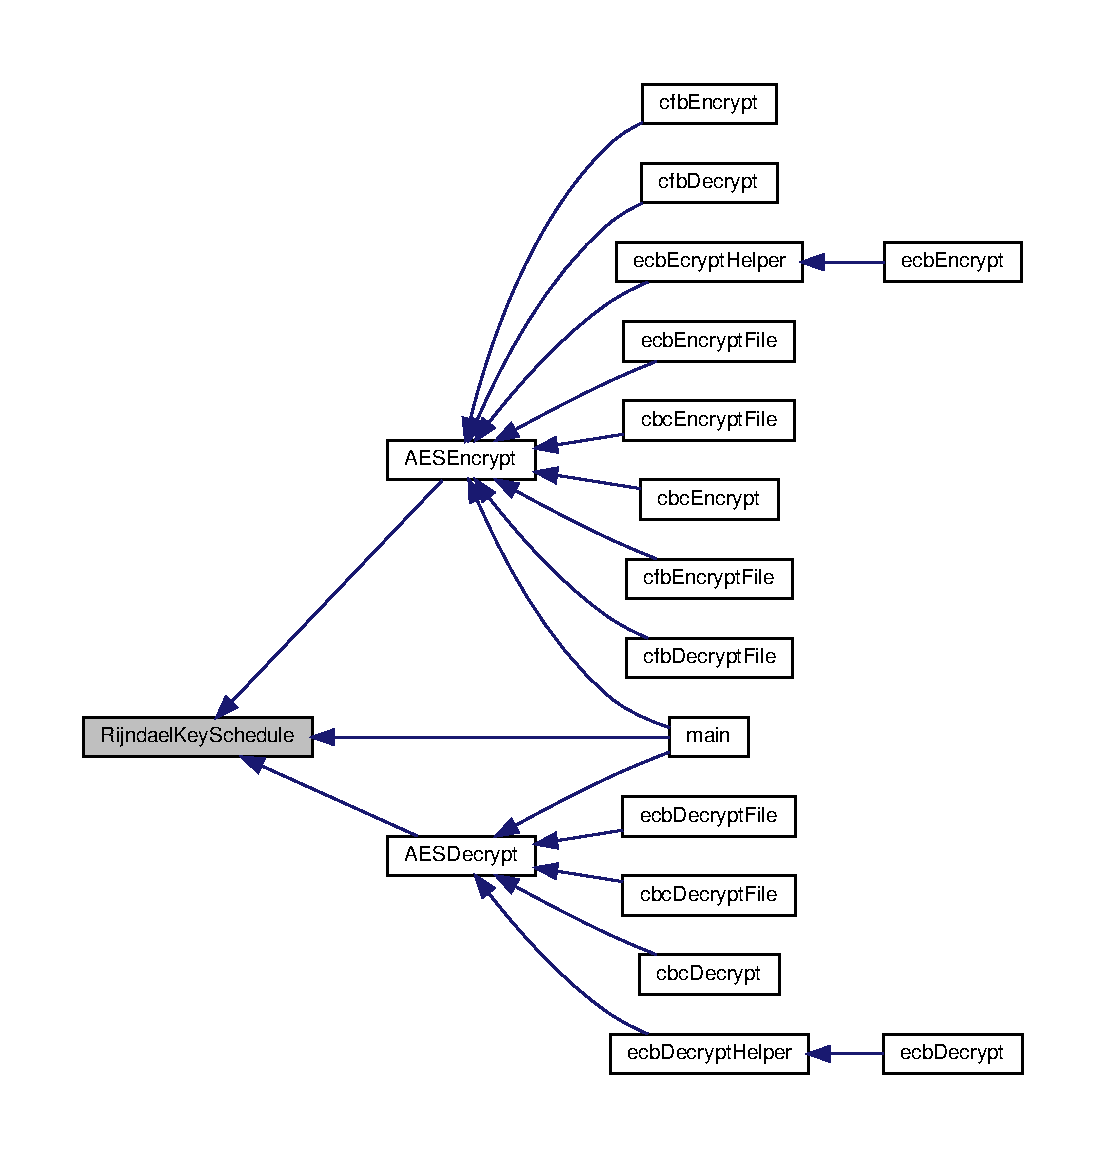
\includegraphics[width=350pt]{_a_e_s_8c_a185c827e4ccbc8e4608e83dfbf9dfc8e_icgraph}
\end{center}
\end{figure}
\mbox{\Hypertarget{_a_e_s_8c_abeb4dba64fcf4d07eac178e732ca6aa8}\label{_a_e_s_8c_abeb4dba64fcf4d07eac178e732ca6aa8}} 
\index{A\+E\+S.\+c@{A\+E\+S.\+c}!Shift\+Rows@{Shift\+Rows}}
\index{Shift\+Rows@{Shift\+Rows}!A\+E\+S.\+c@{A\+E\+S.\+c}}
\subsubsection{\texorpdfstring{Shift\+Rows()}{ShiftRows()}}
{\footnotesize\ttfamily void Shift\+Rows (\begin{DoxyParamCaption}\item[{unsigned char}]{state\mbox{[}4\mbox{]}\mbox{[}4\mbox{]},  }\item[{int}]{word\+Length }\end{DoxyParamCaption})}



Shift\+Rows -\/ Function to shift the state array according to the A\+ES encryption standard for 128 -\/ bits blocks. 


\begin{DoxyParams}{Parameters}
{\em state} & -\/ unsigned char -\/ is the current state of the ciphertext or plaintext during A\+ES encryption or decryption \\
\hline
\end{DoxyParams}


Definition at line 815 of file A\+E\+S.\+c.

Here is the call graph for this function\+:\nopagebreak
\begin{figure}[H]
\begin{center}
\leavevmode
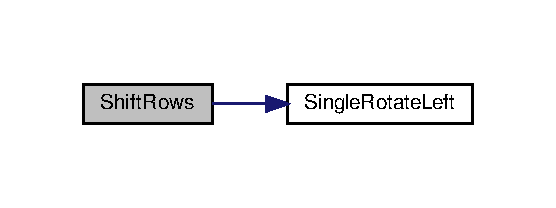
\includegraphics[width=267pt]{_a_e_s_8c_abeb4dba64fcf4d07eac178e732ca6aa8_cgraph}
\end{center}
\end{figure}
Here is the caller graph for this function\+:\nopagebreak
\begin{figure}[H]
\begin{center}
\leavevmode
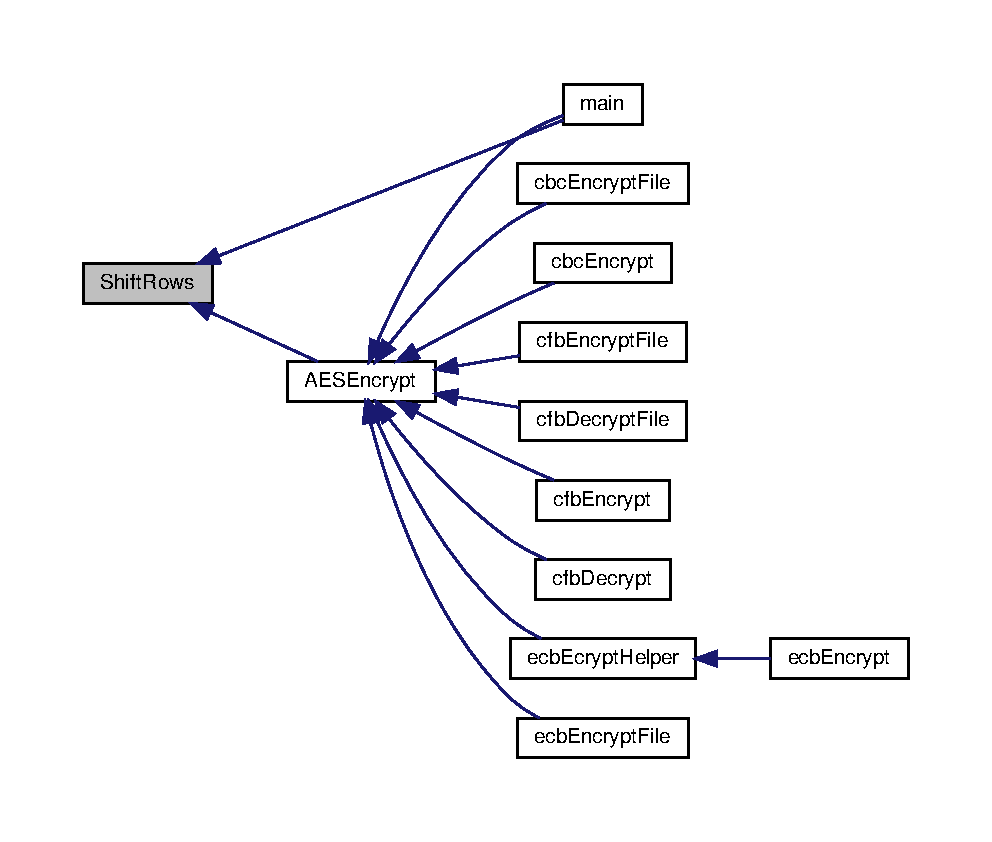
\includegraphics[width=350pt]{_a_e_s_8c_abeb4dba64fcf4d07eac178e732ca6aa8_icgraph}
\end{center}
\end{figure}
\mbox{\Hypertarget{_a_e_s_8c_ac769b0533ccecd203cc3ab64e6b2f950}\label{_a_e_s_8c_ac769b0533ccecd203cc3ab64e6b2f950}} 
\index{A\+E\+S.\+c@{A\+E\+S.\+c}!Single\+Rotate\+Left@{Single\+Rotate\+Left}}
\index{Single\+Rotate\+Left@{Single\+Rotate\+Left}!A\+E\+S.\+c@{A\+E\+S.\+c}}
\subsubsection{\texorpdfstring{Single\+Rotate\+Left()}{SingleRotateLeft()}}
{\footnotesize\ttfamily void Single\+Rotate\+Left (\begin{DoxyParamCaption}\item[{unsigned char $\ast$}]{word,  }\item[{int}]{word\+Length }\end{DoxyParamCaption})}



Single\+Rotate\+Left -\/ Function to rotate the array passed in as a paramter. 


\begin{DoxyParams}{Parameters}
{\em word,a} & single time left (8 bits to the left), with the left most element becoming the right most element. As such\+: rotate(1d2c3a4f) = 2c3a4f1d. \\
\hline
{\em word} & -\/ unsigned char $\ast$word -\/ the array/word to be left rotated by 8 bits. \\
\hline
{\em word\+Length} & -\/ int -\/ length of the parameter \\
\hline
{\em word.} & \\
\hline
\end{DoxyParams}


Definition at line 655 of file A\+E\+S.\+c.

Here is the caller graph for this function\+:\nopagebreak
\begin{figure}[H]
\begin{center}
\leavevmode
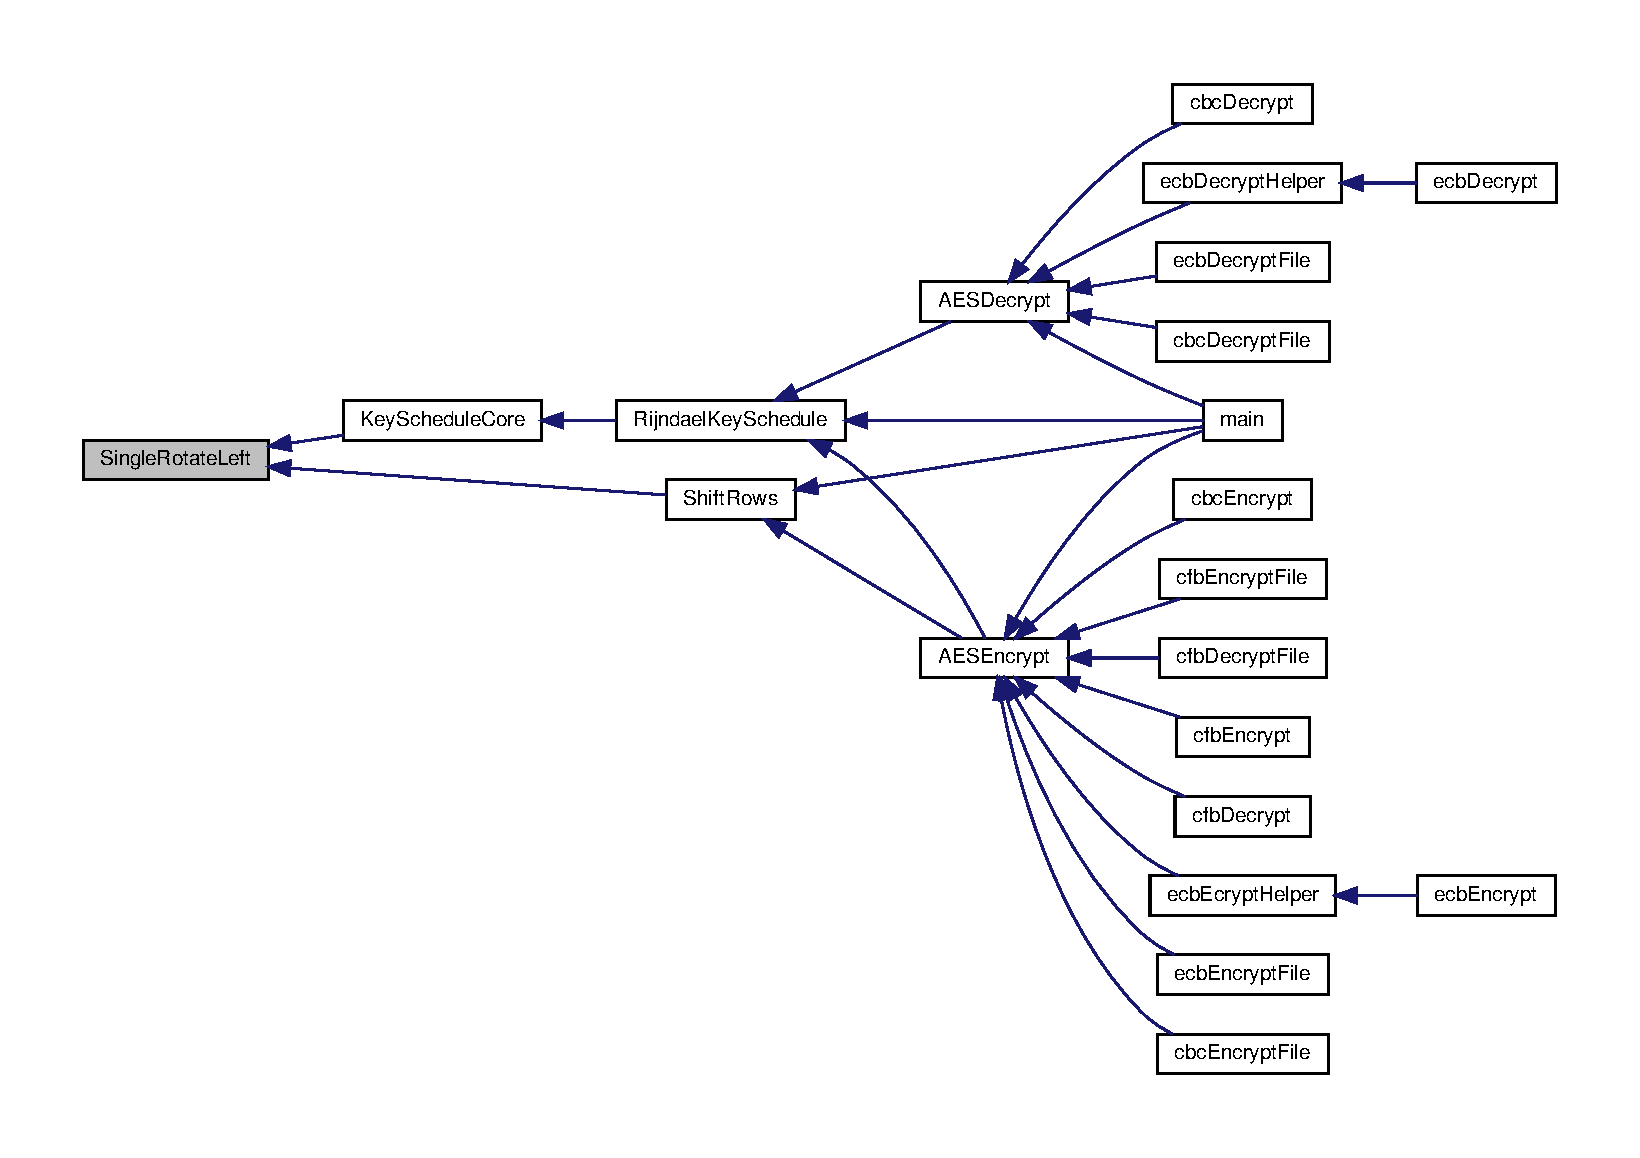
\includegraphics[width=350pt]{_a_e_s_8c_ac769b0533ccecd203cc3ab64e6b2f950_icgraph}
\end{center}
\end{figure}
\mbox{\Hypertarget{_a_e_s_8c_a4fc33ada95d0d2aaea28086aefe173bb}\label{_a_e_s_8c_a4fc33ada95d0d2aaea28086aefe173bb}} 
\index{A\+E\+S.\+c@{A\+E\+S.\+c}!Single\+Rotate\+Right@{Single\+Rotate\+Right}}
\index{Single\+Rotate\+Right@{Single\+Rotate\+Right}!A\+E\+S.\+c@{A\+E\+S.\+c}}
\subsubsection{\texorpdfstring{Single\+Rotate\+Right()}{SingleRotateRight()}}
{\footnotesize\ttfamily void Single\+Rotate\+Right (\begin{DoxyParamCaption}\item[{unsigned char $\ast$}]{word,  }\item[{int}]{word\+Length }\end{DoxyParamCaption})}



Single\+Rotate\+Right -\/ Function to rotate the array passed in as a paramter. 


\begin{DoxyParams}{Parameters}
{\em word,a} & single time right (8 bits to the right), with the right most element becoming the left most element. As such\+: rotate(1d2c3a4f) = 4f1d2c3a.\\
\hline
{\em word} & -\/ unsigned char $\ast$word -\/ the array/word to be right rotated by 8 bits. \\
\hline
{\em word\+Length} & -\/ int -\/ length of the parameter \\
\hline
{\em word.} & \\
\hline
\end{DoxyParams}


Definition at line 857 of file A\+E\+S.\+c.

Here is the caller graph for this function\+:\nopagebreak
\begin{figure}[H]
\begin{center}
\leavevmode
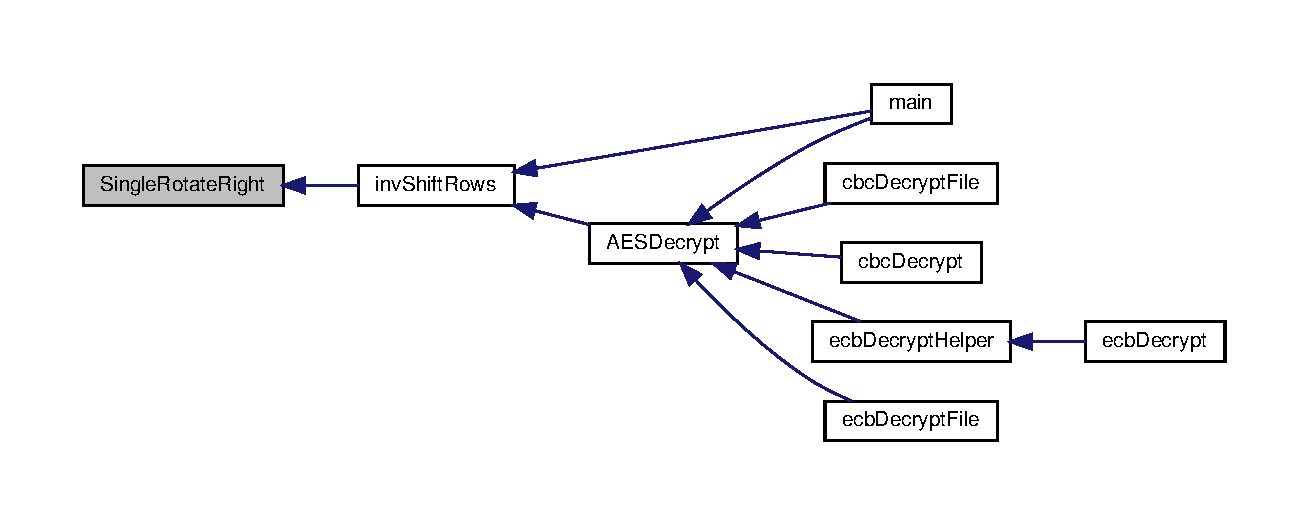
\includegraphics[width=350pt]{_a_e_s_8c_a4fc33ada95d0d2aaea28086aefe173bb_icgraph}
\end{center}
\end{figure}
\mbox{\Hypertarget{_a_e_s_8c_ab066697b473ad5ce74faaceae6def5e5}\label{_a_e_s_8c_ab066697b473ad5ce74faaceae6def5e5}} 
\index{A\+E\+S.\+c@{A\+E\+S.\+c}!strip\+Directory@{strip\+Directory}}
\index{strip\+Directory@{strip\+Directory}!A\+E\+S.\+c@{A\+E\+S.\+c}}
\subsubsection{\texorpdfstring{strip\+Directory()}{stripDirectory()}}
{\footnotesize\ttfamily void strip\+Directory (\begin{DoxyParamCaption}\item[{char $\ast$}]{file\+Name,  }\item[{char $\ast$}]{extracted\+File\+Name,  }\item[{char $\ast$}]{extracted\+File\+Path,  }\item[{int}]{file\+Name\+Length,  }\item[{int}]{slash\+Index }\end{DoxyParamCaption})}



Removes path from the provided path to a file and returns only the file name. 

strip\+Directory -\/ Function that removes path from the provided path to a file and returns only the file name


\begin{DoxyParams}{Parameters}
{\em file\+Name} & The path to a specified file \\
\hline
{\em extracted\+File\+Name} & The name of the file within the provided path to a file \\
\hline
{\em extracted\+File\+Path} & The path to file, excluding the file name \\
\hline
{\em file\+Name\+Length} & The length of the paramter \\
\hline
{\em file\+Name} & \\
\hline
{\em slash\+Index} & The index of the last \textquotesingle{}/\textquotesingle{} in the original file path passed in as a paramter \\
\hline
{\em file\+Name} & \\
\hline
\end{DoxyParams}


Definition at line 1063 of file A\+E\+S.\+c.

Here is the caller graph for this function\+:\nopagebreak
\begin{figure}[H]
\begin{center}
\leavevmode
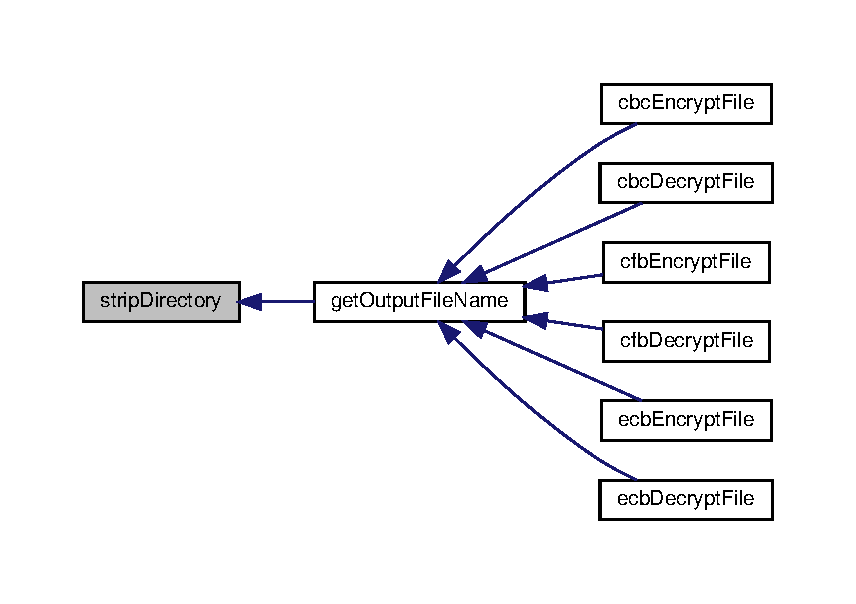
\includegraphics[width=350pt]{_a_e_s_8c_ab066697b473ad5ce74faaceae6def5e5_icgraph}
\end{center}
\end{figure}
\mbox{\Hypertarget{_a_e_s_8c_aec40f89d2cbf831fd0d5d5f1bfa616f5}\label{_a_e_s_8c_aec40f89d2cbf831fd0d5d5f1bfa616f5}} 
\index{A\+E\+S.\+c@{A\+E\+S.\+c}!sub\+Bytes@{sub\+Bytes}}
\index{sub\+Bytes@{sub\+Bytes}!A\+E\+S.\+c@{A\+E\+S.\+c}}
\subsubsection{\texorpdfstring{sub\+Bytes()}{subBytes()}}
{\footnotesize\ttfamily void sub\+Bytes (\begin{DoxyParamCaption}\item[{unsigned char}]{state\mbox{[}4\mbox{]}\mbox{[}4\mbox{]} }\end{DoxyParamCaption})}



sub\+Bytes -\/ Function that performs the sub byte operation where each value is replaced by the s box value 


\begin{DoxyParams}{Parameters}
{\em state} & -\/ unsigned char -\/ is the current state of the ciphertext or plaintext during A\+ES encryption or decryption. \\
\hline
\end{DoxyParams}


Definition at line 789 of file A\+E\+S.\+c.

Here is the call graph for this function\+:\nopagebreak
\begin{figure}[H]
\begin{center}
\leavevmode
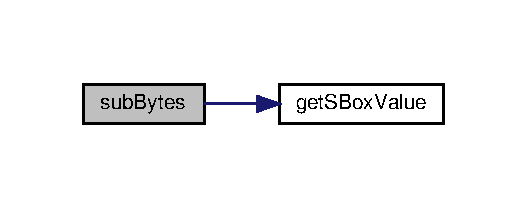
\includegraphics[width=253pt]{_a_e_s_8c_aec40f89d2cbf831fd0d5d5f1bfa616f5_cgraph}
\end{center}
\end{figure}
Here is the caller graph for this function\+:\nopagebreak
\begin{figure}[H]
\begin{center}
\leavevmode
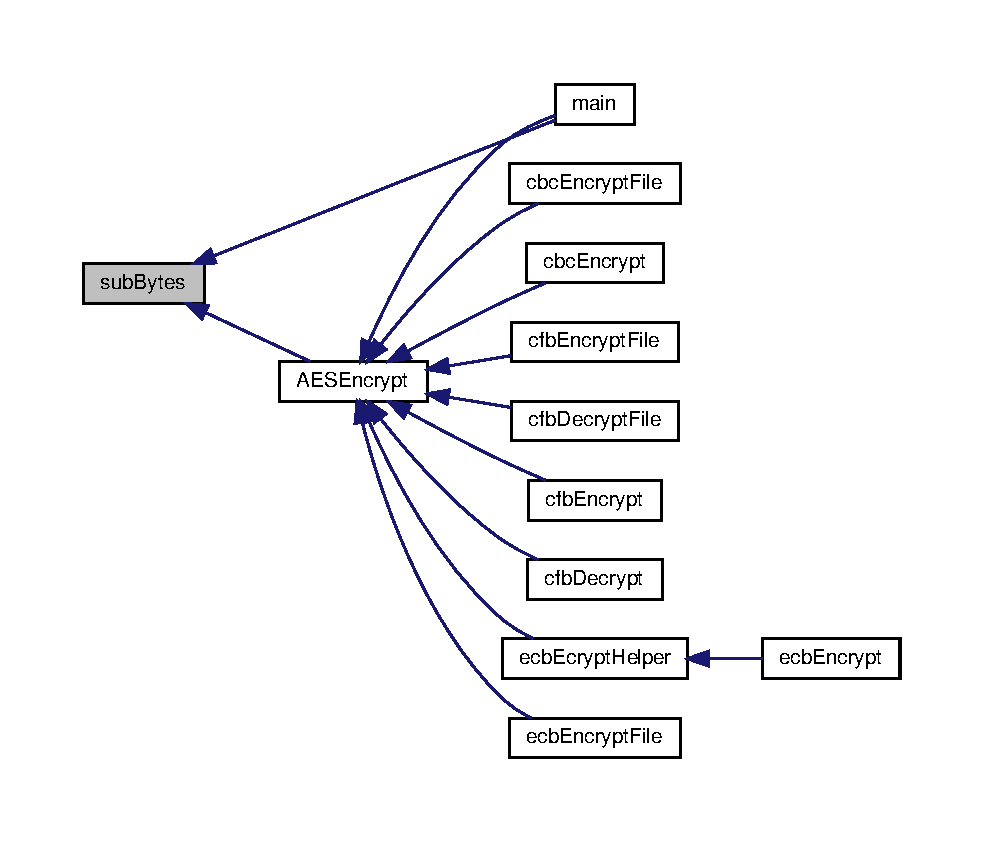
\includegraphics[width=350pt]{_a_e_s_8c_aec40f89d2cbf831fd0d5d5f1bfa616f5_icgraph}
\end{center}
\end{figure}
\mbox{\Hypertarget{_a_e_s_8c_ae01a1e7833d53f19b534e37ace03a691}\label{_a_e_s_8c_ae01a1e7833d53f19b534e37ace03a691}} 
\index{A\+E\+S.\+c@{A\+E\+S.\+c}!validate\+Cipher\+Text\+Length@{validate\+Cipher\+Text\+Length}}
\index{validate\+Cipher\+Text\+Length@{validate\+Cipher\+Text\+Length}!A\+E\+S.\+c@{A\+E\+S.\+c}}
\subsubsection{\texorpdfstring{validate\+Cipher\+Text\+Length()}{validateCipherTextLength()}}
{\footnotesize\ttfamily void validate\+Cipher\+Text\+Length (\begin{DoxyParamCaption}\item[{int}]{cipher\+Text\+Length }\end{DoxyParamCaption})}



validate\+Cipher\+Text\+Length -\/ Function that validates the length of the ciphertext. The validation is done against the A\+E\+S\+\_\+\+B\+L\+O\+C\+K\+\_\+\+S\+I\+ZE value 


\begin{DoxyParams}{Parameters}
{\em cipher\+Text\+Length} & -\/ int -\/ The length of the cipher text as an integer value \\
\hline
\end{DoxyParams}


Definition at line 1015 of file A\+E\+S.\+c.

Here is the caller graph for this function\+:\nopagebreak
\begin{figure}[H]
\begin{center}
\leavevmode
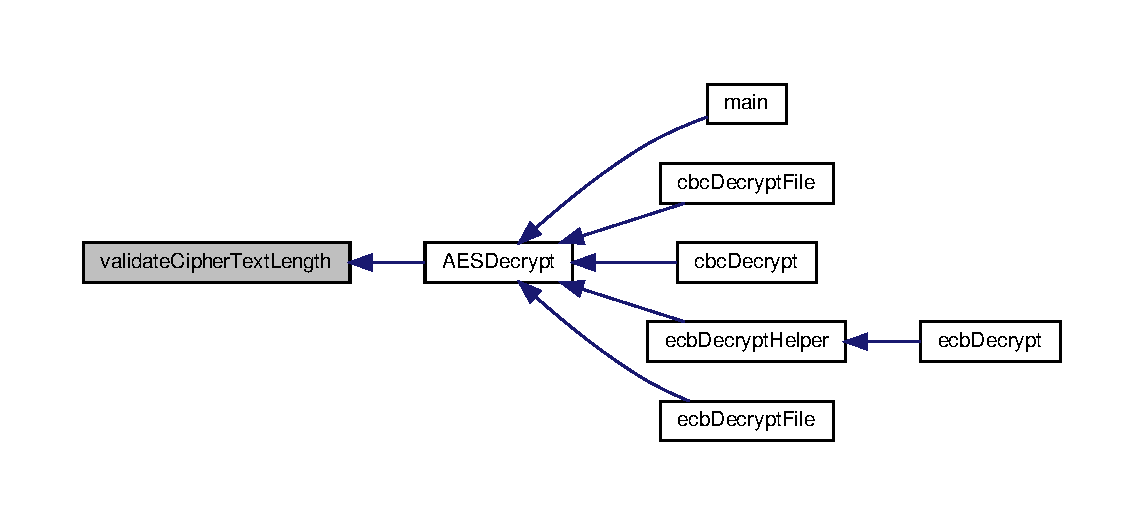
\includegraphics[width=350pt]{_a_e_s_8c_ae01a1e7833d53f19b534e37ace03a691_icgraph}
\end{center}
\end{figure}
\mbox{\Hypertarget{_a_e_s_8c_a0e0b199ded54d7fb53a3bda3fcc02256}\label{_a_e_s_8c_a0e0b199ded54d7fb53a3bda3fcc02256}} 
\index{A\+E\+S.\+c@{A\+E\+S.\+c}!validate\+Num\+Rounds@{validate\+Num\+Rounds}}
\index{validate\+Num\+Rounds@{validate\+Num\+Rounds}!A\+E\+S.\+c@{A\+E\+S.\+c}}
\subsubsection{\texorpdfstring{validate\+Num\+Rounds()}{validateNumRounds()}}
{\footnotesize\ttfamily void validate\+Num\+Rounds (\begin{DoxyParamCaption}\item[{int}]{num\+Rounds,  }\item[{int}]{key\+Length }\end{DoxyParamCaption})}



validate\+Num\+Rounds -\/ Function that validates the number of rounds that have been passed in by the 


\begin{DoxyParams}{Parameters}
{\em num\+Rounds.} & Upon invalid validation, relevent error information will be printed to terminal and the program will exit with an E\+X\+I\+T\+\_\+\+F\+A\+I\+L\+U\+RE flag. \\
\hline
{\em num\+Rounds} & -\/ int -\/ Integer value of the number rounds \\
\hline
\end{DoxyParams}


Definition at line 989 of file A\+E\+S.\+c.

Here is the caller graph for this function\+:\nopagebreak
\begin{figure}[H]
\begin{center}
\leavevmode
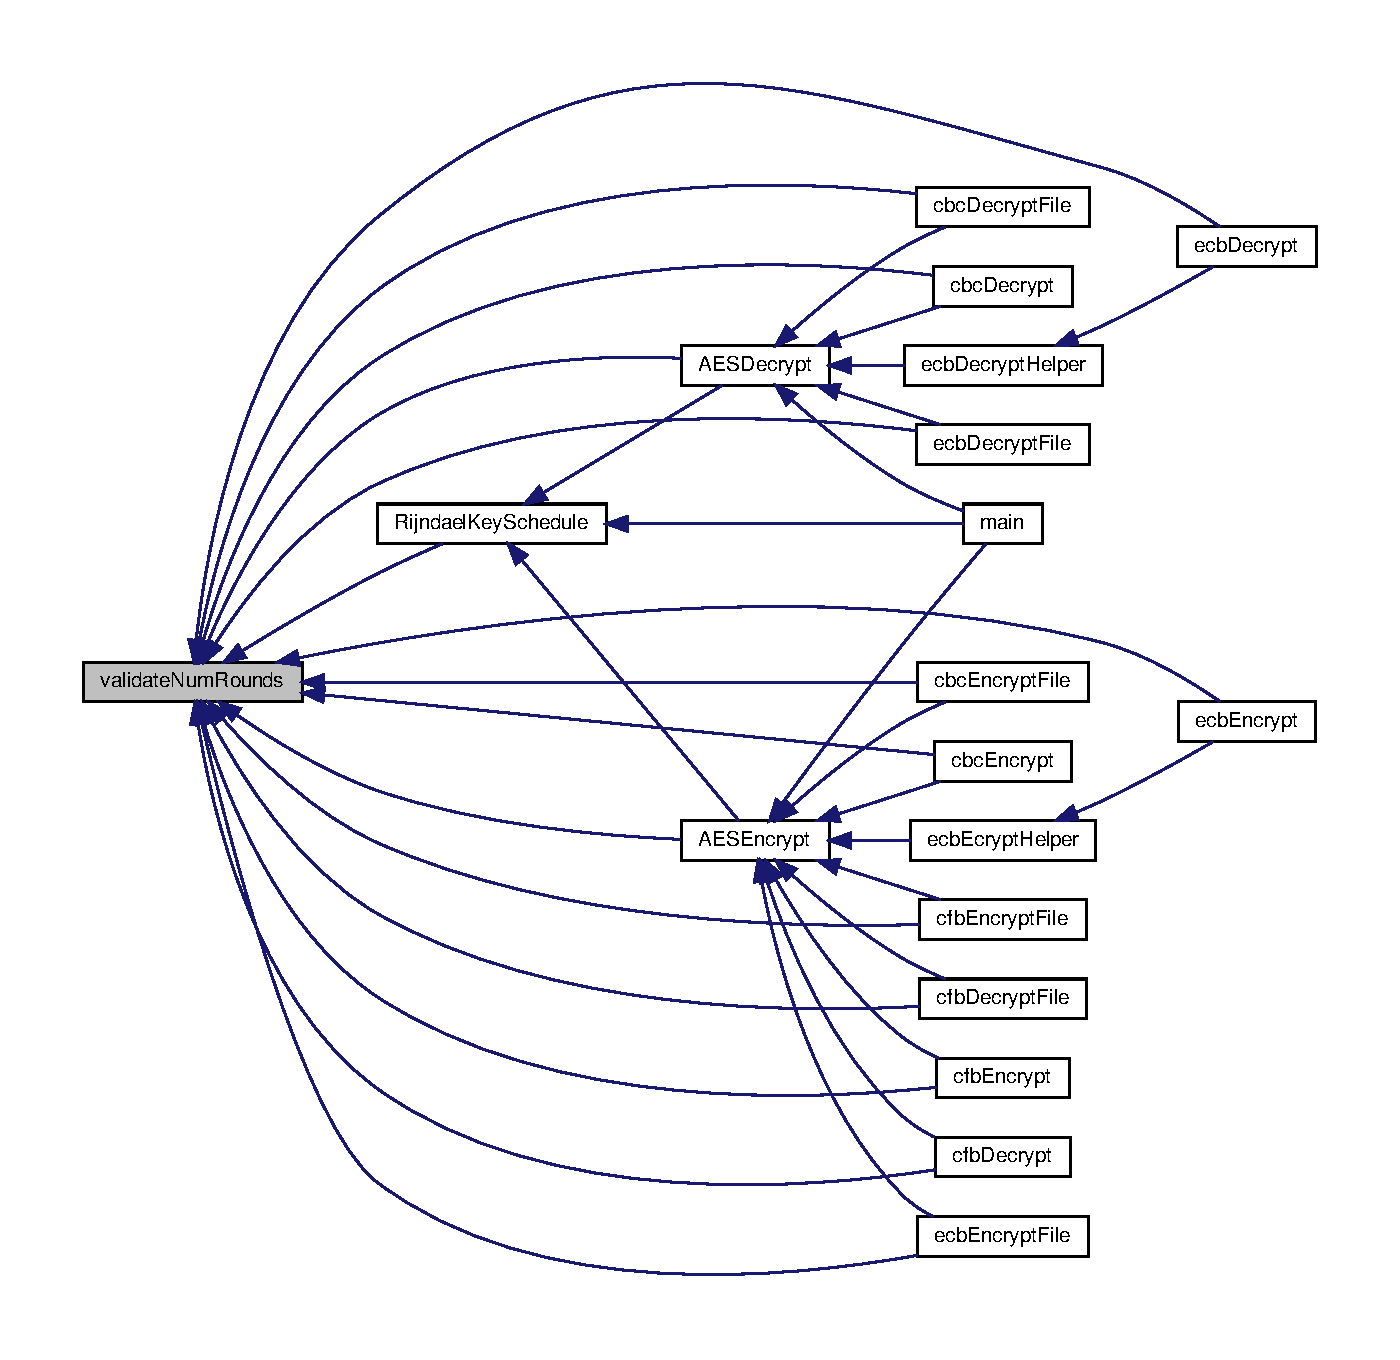
\includegraphics[width=350pt]{_a_e_s_8c_a0e0b199ded54d7fb53a3bda3fcc02256_icgraph}
\end{center}
\end{figure}
\mbox{\Hypertarget{_a_e_s_8c_acefcd728377e1e14187fa8fcd20f4064}\label{_a_e_s_8c_acefcd728377e1e14187fa8fcd20f4064}} 
\index{A\+E\+S.\+c@{A\+E\+S.\+c}!validate\+Plain\+Text\+Length@{validate\+Plain\+Text\+Length}}
\index{validate\+Plain\+Text\+Length@{validate\+Plain\+Text\+Length}!A\+E\+S.\+c@{A\+E\+S.\+c}}
\subsubsection{\texorpdfstring{validate\+Plain\+Text\+Length()}{validatePlainTextLength()}}
{\footnotesize\ttfamily void validate\+Plain\+Text\+Length (\begin{DoxyParamCaption}\item[{size\+\_\+t}]{plain\+Text\+Length }\end{DoxyParamCaption})}



validate\+Plain\+Text\+Length -\/ Function that validates the length of the plaintext. The validation is done against the A\+E\+S\+\_\+\+B\+L\+O\+C\+K\+\_\+\+S\+I\+ZE value 


\begin{DoxyParams}{Parameters}
{\em plain\+Text\+Length} & -\/ int -\/ The length of the plaintext text as an integer value \\
\hline
\end{DoxyParams}


Definition at line 1002 of file A\+E\+S.\+c.

Here is the caller graph for this function\+:\nopagebreak
\begin{figure}[H]
\begin{center}
\leavevmode
\includegraphics[width=350pt]{_a_e_s_8c_acefcd728377e1e14187fa8fcd20f4064_icgraph}
\end{center}
\end{figure}
\mbox{\Hypertarget{_a_e_s_8c_ab601c369ba50730fc02d03bc44aad4e0}\label{_a_e_s_8c_ab601c369ba50730fc02d03bc44aad4e0}} 
\index{A\+E\+S.\+c@{A\+E\+S.\+c}!X\+O\+R\+Blocks@{X\+O\+R\+Blocks}}
\index{X\+O\+R\+Blocks@{X\+O\+R\+Blocks}!A\+E\+S.\+c@{A\+E\+S.\+c}}
\subsubsection{\texorpdfstring{X\+O\+R\+Blocks()}{XORBlocks()}}
{\footnotesize\ttfamily unsigned char$\ast$ X\+O\+R\+Blocks (\begin{DoxyParamCaption}\item[{unsigned char $\ast$}]{block1,  }\item[{unsigned char $\ast$}]{block2,  }\item[{int}]{length }\end{DoxyParamCaption})}



X\+O\+R\+Blocks -\/ Function to X\+OR two blocks of length. 


\begin{DoxyParams}{Parameters}
{\em length} & and retuns the X\+OR\textquotesingle{}d result. User must free the memory returned. \\
\hline
{\em char} & -\/ block1 -\/ First block to be X\+OR\textquotesingle{}d. \\
\hline
{\em char} & -\/ block2 -\/ Second block to be X\+OR\textquotesingle{}d. \\
\hline
{\em length} & -\/ length of the blocks to be X\+OR\textquotesingle{}d. \\
\hline
\end{DoxyParams}
\begin{DoxyReturn}{Returns}
unsigned$\ast$ -\/ Result of the X\+OR. 
\end{DoxyReturn}


Definition at line 1228 of file A\+E\+S.\+c.

Here is the caller graph for this function\+:\nopagebreak
\begin{figure}[H]
\begin{center}
\leavevmode
\includegraphics[width=267pt]{_a_e_s_8c_ab601c369ba50730fc02d03bc44aad4e0_icgraph}
\end{center}
\end{figure}


\subsection{Variable Documentation}
\mbox{\Hypertarget{_a_e_s_8c_ac3c0558617e372fc5ce3648e041e549c}\label{_a_e_s_8c_ac3c0558617e372fc5ce3648e041e549c}} 
\index{A\+E\+S.\+c@{A\+E\+S.\+c}!A\+E\+S\+\_\+\+B\+L\+O\+C\+K\+\_\+\+S\+I\+ZE@{A\+E\+S\+\_\+\+B\+L\+O\+C\+K\+\_\+\+S\+I\+ZE}}
\index{A\+E\+S\+\_\+\+B\+L\+O\+C\+K\+\_\+\+S\+I\+ZE@{A\+E\+S\+\_\+\+B\+L\+O\+C\+K\+\_\+\+S\+I\+ZE}!A\+E\+S.\+c@{A\+E\+S.\+c}}
\subsubsection{\texorpdfstring{A\+E\+S\+\_\+\+B\+L\+O\+C\+K\+\_\+\+S\+I\+ZE}{AES\_BLOCK\_SIZE}}
{\footnotesize\ttfamily const size\+\_\+t A\+E\+S\+\_\+\+B\+L\+O\+C\+K\+\_\+\+S\+I\+ZE = 16}



Variable-\/ const size\+\_\+t A\+E\+S\+\_\+\+B\+L\+O\+C\+K\+\_\+\+S\+I\+ZE. Used to dictate the length in bytes of a single A\+ES block used for encryption and decryption. Set to 16 bytes for a single block. 

Variable -\/ A\+E\+S\+\_\+\+B\+L\+O\+C\+K\+\_\+\+S\+I\+ZE -\/ specifies the length per A\+ES block -\/ 16 bytes. 

Definition at line 24 of file A\+E\+S.\+c.

\mbox{\Hypertarget{_a_e_s_8c_afdaefaa3b28b23dc18709335449a1427}\label{_a_e_s_8c_afdaefaa3b28b23dc18709335449a1427}} 
\index{A\+E\+S.\+c@{A\+E\+S.\+c}!inv\+S\+Box@{inv\+S\+Box}}
\index{inv\+S\+Box@{inv\+S\+Box}!A\+E\+S.\+c@{A\+E\+S.\+c}}
\subsubsection{\texorpdfstring{inv\+S\+Box}{invSBox}}
{\footnotesize\ttfamily const unsigned char inv\+S\+Box\mbox{[}256\mbox{]}}

{\bfseries Initial value\+:}
\begin{DoxyCode}
= \{ 
    
    0x52,0x09,0x6a,0xd5,0x30,0x36,0xa5,0x38,0xbf,0x40,0xa3,0x9e,0x81,0xf3,0xd7,0xfb, 
    0x7c,0xe3,0x39,0x82,0x9b,0x2f,0xff,0x87,0x34,0x8e,0x43,0x44,0xc4,0xde,0xe9,0xcb, 
    0x54,0x7b,0x94,0x32,0xa6,0xc2,0x23,0x3d,0xee,0x4c,0x95,0x0b,0x42,0xfa,0xc3,0x4e, 
    0x08,0x2e,0xa1,0x66,0x28,0xd9,0x24,0xb2,0x76,0x5b,0xa2,0x49,0x6d,0x8b,0xd1,0x25, 
    0x72,0xf8,0xf6,0x64,0x86,0x68,0x98,0x16,0xd4,0xa4,0x5c,0xcc,0x5d,0x65,0xb6,0x92, 
    0x6c,0x70,0x48,0x50,0xfd,0xed,0xb9,0xda,0x5e,0x15,0x46,0x57,0xa7,0x8d,0x9d,0x84, 
    0x90,0xd8,0xab,0x00,0x8c,0xbc,0xd3,0x0a,0xf7,0xe4,0x58,0x05,0xb8,0xb3,0x45,0x06, 
    0xd0,0x2c,0x1e,0x8f,0xca,0x3f,0x0f,0x02,0xc1,0xaf,0xbd,0x03,0x01,0x13,0x8a,0x6b, 
    0x3a,0x91,0x11,0x41,0x4f,0x67,0xdc,0xea,0x97,0xf2,0xcf,0xce,0xf0,0xb4,0xe6,0x73, 
    0x96,0xac,0x74,0x22,0xe7,0xad,0x35,0x85,0xe2,0xf9,0x37,0xe8,0x1c,0x75,0xdf,0x6e, 
    0x47,0xf1,0x1a,0x71,0x1d,0x29,0xc5,0x89,0x6f,0xb7,0x62,0x0e,0xaa,0x18,0xbe,0x1b, 
    0xfc,0x56,0x3e,0x4b,0xc6,0xd2,0x79,0x20,0x9a,0xdb,0xc0,0xfe,0x78,0xcd,0x5a,0xf4, 
    0x1f,0xdd,0xa8,0x33,0x88,0x07,0xc7,0x31,0xb1,0x12,0x10,0x59,0x27,0x80,0xec,0x5f, 
    0x60,0x51,0x7f,0xa9,0x19,0xb5,0x4a,0x0d,0x2d,0xe5,0x7a,0x9f,0x93,0xc9,0x9c,0xef, 
    0xa0,0xe0,0x3b,0x4d,0xae,0x2a,0xf5,0xb0,0xc8,0xeb,0xbb,0x3c,0x83,0x53,0x99,0x61, 
    0x17,0x2b,0x04,0x7e,0xba,0x77,0xd6,0x26,0xe1,0x69,0x14,0x63,0x55,0x21,0x0c,0x7d   \}
\end{DoxyCode}


const unsigned char inv\+S\+Box. Lookup table for the inverse sbox values used during A\+ES Decryption. 



Definition at line 60 of file A\+E\+S.\+c.

\mbox{\Hypertarget{_a_e_s_8c_a58c62505f9b71b2c257046ccf4c9153c}\label{_a_e_s_8c_a58c62505f9b71b2c257046ccf4c9153c}} 
\index{A\+E\+S.\+c@{A\+E\+S.\+c}!Rcon@{Rcon}}
\index{Rcon@{Rcon}!A\+E\+S.\+c@{A\+E\+S.\+c}}
\subsubsection{\texorpdfstring{Rcon}{Rcon}}
{\footnotesize\ttfamily const unsigned char Rcon\mbox{[}255\mbox{]}}

{\bfseries Initial value\+:}
\begin{DoxyCode}
= \{ 
    0x8d, 0x01, 0x02, 0x04, 0x08, 0x10, 0x20, 0x40, 0x80, 0x1b, 0x36, 0x6c, 0xd8,
    0xab, 0x4d, 0x9a, 0x2f, 0x5e, 0xbc, 0x63, 0xc6, 0x97, 0x35, 0x6a, 0xd4, 0xb3,
    0x7d, 0xfa, 0xef, 0xc5, 0x91, 0x39, 0x72, 0xe4, 0xd3, 0xbd, 0x61, 0xc2, 0x9f,
    0x25, 0x4a, 0x94, 0x33, 0x66, 0xcc, 0x83, 0x1d, 0x3a, 0x74, 0xe8, 0xcb, 0x8d,
    0x01, 0x02, 0x04, 0x08, 0x10, 0x20, 0x40, 0x80, 0x1b, 0x36, 0x6c, 0xd8, 0xab,
    0xfa, 0xef, 0xc5, 0x91, 0x39, 0x72, 0xe4, 0xd3, 0xbd, 0x61, 0xc2, 0x9f, 0x25,
    0x4d, 0x9a, 0x2f, 0x5e, 0xbc, 0x63, 0xc6, 0x97, 0x35, 0x6a, 0xd4, 0xb3, 0x7d,
    0x4a, 0x94, 0x33, 0x66, 0xcc, 0x83, 0x1d, 0x3a, 0x74, 0xe8, 0xcb, 0x8d, 0x01,
    0x02, 0x04, 0x08, 0x10, 0x20, 0x40, 0x80, 0x1b, 0x36, 0x6c, 0xd8, 0xab, 0x4d,
    0x9a, 0x2f, 0x5e, 0xbc, 0x63, 0xc6, 0x97, 0x35, 0x6a, 0xd4, 0xb3, 0x7d, 0xfa,
    0xef, 0xc5, 0x91, 0x39, 0x72, 0xe4, 0xd3, 0xbd, 0x61, 0xc2, 0x9f, 0x25, 0x4a,
    0x94, 0x33, 0x66, 0xcc, 0x83, 0x1d, 0x3a, 0x74, 0xe8, 0xcb, 0x8d, 0x01, 0x02,
    0x04, 0x08, 0x10, 0x20, 0x40, 0x80, 0x1b, 0x36, 0x6c, 0xd8, 0xab, 0x4d, 0x9a,
    0x2f, 0x5e, 0xbc, 0x63, 0xc6, 0x97, 0x35, 0x6a, 0xd4, 0xb3, 0x7d, 0xfa, 0xef,
    0xc5, 0x91, 0x39, 0x72, 0xe4, 0xd3, 0xbd, 0x61, 0xc2, 0x9f, 0x25, 0x4a, 0x94,
    0x33, 0x66, 0xcc, 0x83, 0x1d, 0x3a, 0x74, 0xe8, 0xcb, 0x8d, 0x01, 0x02, 0x04,
    0x08, 0x10, 0x20, 0x40, 0x80, 0x1b, 0x36, 0x6c, 0xd8, 0xab, 0x4d, 0x9a, 0x2f,
    0x5e, 0xbc, 0x63, 0xc6, 0x97, 0x35, 0x6a, 0xd4, 0xb3, 0x7d, 0xfa, 0xef, 0xc5,
    0x91, 0x39, 0x72, 0xe4, 0xd3, 0xbd, 0x61, 0xc2, 0x9f, 0x25, 0x4a, 0x94, 0x33,
    0x66, 0xcc, 0x83, 0x1d, 0x3a, 0x74, 0xe8, 0xcb \}
\end{DoxyCode}


const unsigned char Rcon. Lookup table for the Rcon values used during Rijndael Key Schedule during the A\+ES Encryption and Decryption. 



Definition at line 83 of file A\+E\+S.\+c.

\mbox{\Hypertarget{_a_e_s_8c_abbb6f385c467cfd964a68eeb6caaa04f}\label{_a_e_s_8c_abbb6f385c467cfd964a68eeb6caaa04f}} 
\index{A\+E\+S.\+c@{A\+E\+S.\+c}!sbox@{sbox}}
\index{sbox@{sbox}!A\+E\+S.\+c@{A\+E\+S.\+c}}
\subsubsection{\texorpdfstring{sbox}{sbox}}
{\footnotesize\ttfamily const unsigned char sbox\mbox{[}256\mbox{]}}

{\bfseries Initial value\+:}
\begin{DoxyCode}
= \{
    
    0x63, 0x7c, 0x77, 0x7b, 0xf2, 0x6b, 0x6f, 0xc5, 0x30, 0x01, 0x67, 0x2b, 0xfe, 0xd7, 0xab, 0x76,     
    0xca, 0x82, 0xc9, 0x7d, 0xfa, 0x59, 0x47, 0xf0, 0xad, 0xd4, 0xa2, 0xaf, 0x9c, 0xa4, 0x72, 0xc0,     
    0xb7, 0xfd, 0x93, 0x26, 0x36, 0x3f, 0xf7, 0xcc, 0x34, 0xa5, 0xe5, 0xf1, 0x71, 0xd8, 0x31, 0x15,     
    0x04, 0xc7, 0x23, 0xc3, 0x18, 0x96, 0x05, 0x9a, 0x07, 0x12, 0x80, 0xe2, 0xeb, 0x27, 0xb2, 0x75,     
    0x09, 0x83, 0x2c, 0x1a, 0x1b, 0x6e, 0x5a, 0xa0, 0x52, 0x3b, 0xd6, 0xb3, 0x29, 0xe3, 0x2f, 0x84,     
    0x53, 0xd1, 0x00, 0xed, 0x20, 0xfc, 0xb1, 0x5b, 0x6a, 0xcb, 0xbe, 0x39, 0x4a, 0x4c, 0x58, 0xcf,     
    0xd0, 0xef, 0xaa, 0xfb, 0x43, 0x4d, 0x33, 0x85, 0x45, 0xf9, 0x02, 0x7f, 0x50, 0x3c, 0x9f, 0xa8,     
    0x51, 0xa3, 0x40, 0x8f, 0x92, 0x9d, 0x38, 0xf5, 0xbc, 0xb6, 0xda, 0x21, 0x10, 0xff, 0xf3, 0xd2,     
    0xcd, 0x0c, 0x13, 0xec, 0x5f, 0x97, 0x44, 0x17, 0xc4, 0xa7, 0x7e, 0x3d, 0x64, 0x5d, 0x19, 0x73,     
    0x60, 0x81, 0x4f, 0xdc, 0x22, 0x2a, 0x90, 0x88, 0x46, 0xee, 0xb8, 0x14, 0xde, 0x5e, 0x0b, 0xdb,     
    0xe0, 0x32, 0x3a, 0x0a, 0x49, 0x06, 0x24, 0x5c, 0xc2, 0xd3, 0xac, 0x62, 0x91, 0x95, 0xe4, 0x79,     
    0xe7, 0xc8, 0x37, 0x6d, 0x8d, 0xd5, 0x4e, 0xa9, 0x6c, 0x56, 0xf4, 0xea, 0x65, 0x7a, 0xae, 0x08,     
    0xba, 0x78, 0x25, 0x2e, 0x1c, 0xa6, 0xb4, 0xc6, 0xe8, 0xdd, 0x74, 0x1f, 0x4b, 0xbd, 0x8b, 0x8a,     
    0x70, 0x3e, 0xb5, 0x66, 0x48, 0x03, 0xf6, 0x0e, 0x61, 0x35, 0x57, 0xb9, 0x86, 0xc1, 0x1d, 0x9e,     
    0xe1, 0xf8, 0x98, 0x11, 0x69, 0xd9, 0x8e, 0x94, 0x9b, 0x1e, 0x87, 0xe9, 0xce, 0x55, 0x28, 0xdf,     
    0x8c, 0xa1, 0x89, 0x0d, 0xbf, 0xe6, 0x42, 0x68, 0x41, 0x99, 0x2d, 0x0f, 0xb0, 0x54, 0xbb, 0x16 \}
\end{DoxyCode}


const unsigned char sbox. Lookup table for the sbox values used during A\+ES Encryption. 



Definition at line 37 of file A\+E\+S.\+c.

\mbox{\Hypertarget{_a_e_s_8c_a48113b3faee8aad8efa17aac0b56b63b}\label{_a_e_s_8c_a48113b3faee8aad8efa17aac0b56b63b}} 
\index{A\+E\+S.\+c@{A\+E\+S.\+c}!V\+E\+R\+B\+O\+SE@{V\+E\+R\+B\+O\+SE}}
\index{V\+E\+R\+B\+O\+SE@{V\+E\+R\+B\+O\+SE}!A\+E\+S.\+c@{A\+E\+S.\+c}}
\subsubsection{\texorpdfstring{V\+E\+R\+B\+O\+SE}{VERBOSE}}
{\footnotesize\ttfamily size\+\_\+t V\+E\+R\+B\+O\+SE = 0}



Variable-\/ size\+\_\+t V\+E\+R\+B\+O\+SE Used to dictate whether verbose output is printed to the terminal or not. If 0, does not print verbose. If 1, prints verbose. 

Variable -\/ V\+E\+R\+B\+O\+SE -\/ specifies if verbose output should be printed or not. 

Definition at line 31 of file A\+E\+S.\+c.


\hypertarget{_a_e_s_8h}{}\section{A\+E\+S.\+h File Reference}
\label{_a_e_s_8h}\index{A\+E\+S.\+h@{A\+E\+S.\+h}}


A\+ES encryption and decryption module header file. This file contains the function headers for the functions used for A\+ES encryption and decryption. Input must be A\+S\+C\+II and not hex. The functions implemented in this file, perform the A\+ES encryption and decryption on a single block of size dictated by the variable A\+E\+S\+\_\+\+B\+L\+O\+C\+K\+\_\+\+S\+I\+ZE.  


{\ttfamily \#include $<$stdio.\+h$>$}\newline
{\ttfamily \#include $<$stdint.\+h$>$}\newline
{\ttfamily \#include $<$string.\+h$>$}\newline
{\ttfamily \#include $<$stdlib.\+h$>$}\newline
{\ttfamily \#include $<$stdbool.\+h$>$}\newline
Include dependency graph for A\+E\+S.\+h\+:\nopagebreak
\begin{figure}[H]
\begin{center}
\leavevmode
\includegraphics[width=350pt]{_a_e_s_8h__incl}
\end{center}
\end{figure}
This graph shows which files directly or indirectly include this file\+:\nopagebreak
\begin{figure}[H]
\begin{center}
\leavevmode
\includegraphics[width=350pt]{_a_e_s_8h__dep__incl}
\end{center}
\end{figure}
\subsection*{Functions}
\begin{DoxyCompactItemize}
\item 
int \hyperlink{_a_e_s_8h_ab7583f82c95236839316097a3baf8e21}{get\+Num\+Rounds} (int)
\begin{DoxyCompactList}\small\item\em get\+Num\+Rounds -\/ Function to return the number of rounds of A\+ES encryption and decryption based off of the length of the key given in \end{DoxyCompactList}\item 
unsigned char $\ast$ \hyperlink{_a_e_s_8h_a0ac21e951d3e46598708ab8fd8bc61c5}{A\+E\+S\+Encrypt} (unsigned char $\ast$, unsigned char $\ast$, int, int)
\begin{DoxyCompactList}\small\item\em A\+E\+S\+Encrypt -\/ Function to encrypt a single block of plaintext passed in as parameter  plain\+Text using A\+ES encryption, for 128, 192 and 256 bit keys. Validates the keylength and returns the corresponding ciphertext. The caller of the function must ensure that the returned ciphertext pointer is freed. The ciphertext returned is always 16 bytes and the plain\+Text must be 16 bytes or less. Makes use of zero padding. All input must be in A\+S\+C\+II and N\+OT hex. \end{DoxyCompactList}\item 
unsigned char $\ast$ \hyperlink{_a_e_s_8h_aea7dd7439aa08f23e6fecd32d4055ac3}{A\+E\+S\+Decrypt} (unsigned char $\ast$, unsigned char $\ast$, int, int)
\begin{DoxyCompactList}\small\item\em A\+E\+S\+Decrypt -\/ Function to decrypt a single block of ciphertext passed in as parameter  cipher\+Text using A\+ES decryption, for 128, 192 and 256 bit keys. Validates the keylength and returns the corresponding plaintext. The caller of the function must ensure that the returned plaintext pointer is freed. The plaintext returned is always 16 bytes and the plain\+Text must be 16 bytes or less. Makes use of zero padding. All input must be in A\+S\+C\+II and N\+OT hex. \end{DoxyCompactList}\item 
unsigned char $\ast$ \hyperlink{_a_e_s_8h_a53bffc877a08f01e5fd9cf1e28298aab}{Rijndael\+Key\+Schedule} (unsigned char $\ast$, int)
\begin{DoxyCompactList}\small\item\em Rijndael\+Key\+Schedule -\/ Function that performs the Rijndael key scheduling for A\+ES encryption. Takes in the original key passed in as parameter. \end{DoxyCompactList}\item 
void \hyperlink{_a_e_s_8h_aa2c2bbef104b3d3e4c4851ca338ffb8c}{print\+State\+Array} (uint8\+\_\+t\mbox{[}4\mbox{]}\mbox{[}4\mbox{]})
\begin{DoxyCompactList}\small\item\em print\+State\+Array -\/ Function to print the state array to the terminal in hex format. \end{DoxyCompactList}\item 
unsigned char \hyperlink{_a_e_s_8h_a6692cb12e0e4495fbba5cb07af94e20d}{get\+S\+Box\+Value} (unsigned char)
\begin{DoxyCompactList}\small\item\em get\+S\+Box\+Value -\/ Function to return the s\+Box value passed in as a parameter \end{DoxyCompactList}\item 
unsigned char \hyperlink{_a_e_s_8h_a533c79baa5917f8daa5ef751b87dc6b9}{get\+Inv\+S\+Box} (unsigned char)
\begin{DoxyCompactList}\small\item\em get\+Inv\+S\+Box -\/ Function to return the inverse s\+Box value passed in as a parameter \end{DoxyCompactList}\item 
unsigned char \hyperlink{_a_e_s_8h_af2da93be75f2ce31bfd9c7b18dcd3642}{get\+Rcon\+Value} (unsigned char)
\begin{DoxyCompactList}\small\item\em get\+Rcon\+Value -\/ Function to return the Rcon value for the index passed in as a parameter \end{DoxyCompactList}\item 
void \hyperlink{_a_e_s_8h_a772c8b1e9ef554b5c2d995ae5834cc3b}{Single\+Rotate\+Left} (unsigned char $\ast$, int)
\begin{DoxyCompactList}\small\item\em Single\+Rotate\+Left -\/ Function to rotate the array passed in as a paramter. \end{DoxyCompactList}\item 
void \hyperlink{_a_e_s_8h_a4d8c6f749326403dce59fae3f81cd120}{Key\+Schedule\+Core} (unsigned char $\ast$, int, int)
\begin{DoxyCompactList}\small\item\em Key\+Schedule\+Core -\/ Function that performs the key schedule core for the Rijndael Key Schedule. Performs a single rotate left of the word passed in as. \end{DoxyCompactList}\item 
void \hyperlink{_a_e_s_8h_a3171e930e8e63e937e3542740b7c94d6}{Shift\+Rows} (unsigned char\mbox{[}4\mbox{]}\mbox{[}4\mbox{]}, int)
\begin{DoxyCompactList}\small\item\em Shift\+Rows -\/ Function to shift the state array according to the A\+ES encryption standard for 128 -\/ bits blocks. \end{DoxyCompactList}\item 
void \hyperlink{_a_e_s_8h_a6674963eab83fe4573ea8b5ee36728ad}{Add\+Round\+Key} (unsigned char\mbox{[}4\mbox{]}\mbox{[}4\mbox{]}, unsigned char\mbox{[}4\mbox{]}\mbox{[}4\mbox{]})
\begin{DoxyCompactList}\small\item\em Add\+Round\+Key -\/ Function that performs the Bitwise X\+OR between state and key as per A\+ES encryption. \end{DoxyCompactList}\item 
void \hyperlink{_a_e_s_8h_a07eae9e44f492880e0a0fb59edb17d34}{sub\+Bytes} (unsigned char\mbox{[}4\mbox{]}\mbox{[}4\mbox{]})
\begin{DoxyCompactList}\small\item\em sub\+Bytes -\/ Function that performs the sub byte operation where each value is replaced by the s box value \end{DoxyCompactList}\item 
void \hyperlink{_a_e_s_8h_adef9f30a148bc7732de37901f741ba5e}{mix\+Columns} (unsigned char\mbox{[}4\mbox{]}\mbox{[}4\mbox{]})
\begin{DoxyCompactList}\small\item\em mix\+Columns -\/ Function that performs the Mix\+Columns step of A\+ES as specified by A\+ES encryption. \end{DoxyCompactList}\item 
void \hyperlink{_a_e_s_8h_abbaab65a86e18c20ed73cb7f712e0eed}{inv\+Sub\+Bytes} (unsigned char\mbox{[}4\mbox{]}\mbox{[}4\mbox{]})
\begin{DoxyCompactList}\small\item\em inv\+Sub\+Bytes -\/ Function that performs the inverse of Function sub\+Bytes \end{DoxyCompactList}\item 
void \hyperlink{_a_e_s_8h_a0b8bd9c3f028f65310f63598410d816b}{inv\+Shift\+Rows} (unsigned char\mbox{[}4\mbox{]}\mbox{[}4\mbox{]}, int)
\begin{DoxyCompactList}\small\item\em inv\+Shift\+Rows -\/ Function to shift the state array Inverse according to the A\+ES encryption standard for 128 -\/ bits blocks \end{DoxyCompactList}\item 
void \hyperlink{_a_e_s_8h_ab94b816921097af452b3bcf62c701258}{Single\+Rotate\+Right} (unsigned char $\ast$, int)
\begin{DoxyCompactList}\small\item\em Single\+Rotate\+Right -\/ Function to rotate the array passed in as a paramter. \end{DoxyCompactList}\item 
int \hyperlink{_a_e_s_8h_a65882384e88b16eb2b875f28119bfa71}{get\+Padded\+Key\+Length} (int)
\begin{DoxyCompactList}\small\item\em get\+Padded\+Key\+Length -\/ Function to return a valid key length (in bytes) based off of the current key length passed in as \end{DoxyCompactList}\item 
void \hyperlink{_a_e_s_8h_a15e43c925ddfb0fcc1e4a6138962ce68}{inv\+Mix\+Columns} (unsigned char\mbox{[}4\mbox{]}\mbox{[}4\mbox{]})
\begin{DoxyCompactList}\small\item\em inv\+Mix\+Columns -\/ Function that does the inverse of the Mix Column Step for A\+ES Encryption. Performs the gallois field multiplication and the required X\+OR to the state passed in as a paramter \end{DoxyCompactList}\item 
unsigned char \hyperlink{_a_e_s_8h_a3d380a2242622d7f06999c772b6f09eb}{gallois\+Field\+Mult} (unsigned char, unsigned char)
\begin{DoxyCompactList}\small\item\em gallois\+Field\+Mult -\/ Function to perform the Galois field multiplication operation required for the inverse mix columns and the mix columns operation of the A\+ES encryption and decryption processes. Returns the result of the multiplication. \end{DoxyCompactList}\item 
void \hyperlink{_a_e_s_8h_a66cd2ce21006225467c842eb708f7923}{get\+Round\+Key} (unsigned char $\ast$, unsigned char $\ast$, int)
\begin{DoxyCompactList}\small\item\em get\+Round\+Key -\/ Function to extract the correct sub-\/key to use for the appropriate round specified by \end{DoxyCompactList}\item 
void \hyperlink{_a_e_s_8h_a997ca47a4474fdb26b9bdbdcef4b734c}{construct\+State\+Array} (unsigned char $\ast$, unsigned char\mbox{[}$\,$\mbox{]}\mbox{[}4\mbox{]})
\begin{DoxyCompactList}\small\item\em construct\+State\+Array -\/ Function to convert the state array from a flat 1D array to a multidimensional array. \end{DoxyCompactList}\item 
uint8\+\_\+t \hyperlink{_a_e_s_8h_a7b4ba0ba076b29e7eca94cc3bcba9f9d}{hex\+To\+Int} (char c)
\begin{DoxyCompactList}\small\item\em hex\+To\+Int -\/ Function that converts a given hex value into an integer. \end{DoxyCompactList}\item 
uint8\+\_\+t \hyperlink{_a_e_s_8h_acb25fd10b0e1c3e0844d4bde447259de}{hex\+To\+Ascii} (char c, char d)
\begin{DoxyCompactList}\small\item\em hex\+To\+Ascii -\/ Function that converts a given hex value to its A\+S\+C\+II equivalent. \end{DoxyCompactList}\item 
void \hyperlink{_a_e_s_8h_a69dcfd00e48471cb60dc1b24ba6e5520}{hex\+To\+Ascii\+String} (char $\ast$str, char $\ast$done, int)
\begin{DoxyCompactList}\small\item\em hex\+To\+Ascii\+String -\/ Function that converts a given string of hex values into its A\+S\+C\+II equivalent. A hex string contains hex chars and is \char`\"{}encoded\char`\"{} in ascii In order to encrypt it, it must be converted to the equivalent ascii plain text string plaintext string is half the size of hex, since two hex chars = 1 ascii char if hex string is \char`\"{}4\+A\char`\"{} it will be converted to \char`\"{}\+J\char`\"{} in ascii which will have a hex representation of \char`\"{}4a\char`\"{} The original hex string converted to hex staright or printed in hex straight rather will print or have the value \char`\"{}0x34\char`\"{}, \char`\"{}0x31\char`\"{} B\+A\+S\+I\+C\+A\+L\+LY T\+HE H\+EX S\+T\+R\+I\+NG FF IS I\+N\+T\+E\+R\+P\+R\+E\+T\+ED AS T\+HE C\+H\+A\+RS FF, whereas when using this function we intend it to be \char`\"{}\+J\char`\"{}, ie the char \char`\"{}\+J\char`\"{} \end{DoxyCompactList}\item 
unsigned char $\ast$ \hyperlink{_a_e_s_8h_ac189aee6672718650020cf627d45c780}{ascii\+To\+Hex\+String} (unsigned char $\ast$ascii\+String, unsigned char $\ast$hex\+String, size\+\_\+t ascii\+String\+Len)
\begin{DoxyCompactList}\small\item\em Function name\+: ascii\+To\+Hex\+String -\/ convert an ascii String to an ascii string. \end{DoxyCompactList}\item 
void \hyperlink{_a_e_s_8h_a0e0b199ded54d7fb53a3bda3fcc02256}{validate\+Num\+Rounds} (int num\+Rounds, int key\+Length)
\begin{DoxyCompactList}\small\item\em validate\+Num\+Rounds -\/ Function that validates the number of rounds that have been passed in by the \end{DoxyCompactList}\item 
void \hyperlink{_a_e_s_8h_acefcd728377e1e14187fa8fcd20f4064}{validate\+Plain\+Text\+Length} (size\+\_\+t plain\+Text\+Length)
\begin{DoxyCompactList}\small\item\em validate\+Plain\+Text\+Length -\/ Function that validates the length of the plaintext. The validation is done against the A\+E\+S\+\_\+\+B\+L\+O\+C\+K\+\_\+\+S\+I\+ZE value \end{DoxyCompactList}\item 
void \hyperlink{_a_e_s_8h_ae01a1e7833d53f19b534e37ace03a691}{validate\+Cipher\+Text\+Length} (int cipher\+Text\+Length)
\begin{DoxyCompactList}\small\item\em validate\+Cipher\+Text\+Length -\/ Function that validates the length of the ciphertext. The validation is done against the A\+E\+S\+\_\+\+B\+L\+O\+C\+K\+\_\+\+S\+I\+ZE value \end{DoxyCompactList}\item 
void \hyperlink{_a_e_s_8h_a0b24eb7a5fd67e9fcd9e21711630e86c}{print\+A\+E\+S\+Block} (unsigned char $\ast$temp)
\begin{DoxyCompactList}\small\item\em print\+A\+E\+S\+Block -\/ Function to print a single block in hex format to the terminal. \end{DoxyCompactList}\item 
int \hyperlink{_a_e_s_8h_a9dcad0047890de22f3d15611a10ab74f}{file\+Name\+Dir\+Index} (char $\ast$file\+Name, int file\+Name\+Length)
\begin{DoxyCompactList}\small\item\em Returns the last index of \textquotesingle{}/\textquotesingle{} in a given path, otherwise returns -\/1 if no \textquotesingle{}/\textquotesingle{} is found. \end{DoxyCompactList}\item 
void \hyperlink{_a_e_s_8h_ab066697b473ad5ce74faaceae6def5e5}{strip\+Directory} (char $\ast$file\+Name, char $\ast$extracted\+File\+Name, char $\ast$extracted\+File\+Path, int file\+Name\+Length, int slash\+Index)
\begin{DoxyCompactList}\small\item\em strip\+Directory -\/ Function that removes path from the provided path to a file and returns only the file name \end{DoxyCompactList}\item 
void \hyperlink{_a_e_s_8h_ac206e95e4e98f7a5a92b046ad726f622}{get\+Output\+File\+Name} (int type, char $\ast$file\+Name, char $\ast$output\+File\+Name, char $\ast$)
\begin{DoxyCompactList}\small\item\em Get the output file name from all the parameters passed in. \end{DoxyCompactList}\item 
uint8\+\_\+t \hyperlink{_a_e_s_8h_a3bf513612c15693c3b2be10b94298e05}{is\+File\+Txt} (unsigned char $\ast$file\+Name)
\begin{DoxyCompactList}\small\item\em is\+File\+Txt -\/ Function to determine if the file passed in as a paramter \end{DoxyCompactList}\item 
unsigned char $\ast$ \hyperlink{_a_e_s_8h_afba897e91364663f883cc51ed309dc92}{key\+Hex\+To\+Ascii} (unsigned char $\ast$hex\+Key, int key\+Length)
\begin{DoxyCompactList}\small\item\em key\+Hex\+To\+Ascii -\/ Function to convert a key from a Hex string passed in as a paramter \end{DoxyCompactList}\item 
unsigned char $\ast$ \hyperlink{_a_e_s_8h_ad82d1b77336ac1292ed5a24b92380f42}{I\+V\+Hex\+To\+Ascii} (unsigned char $\ast$hex\+IV, int I\+V\+Length)
\begin{DoxyCompactList}\small\item\em I\+V\+Hex\+To\+Ascii -\/ Function to convert a initialization vector from a Hex string passed in as a paramter. \end{DoxyCompactList}\item 
unsigned char $\ast$ \hyperlink{_a_e_s_8h_ab601c369ba50730fc02d03bc44aad4e0}{X\+O\+R\+Blocks} (unsigned char $\ast$block1, unsigned char $\ast$block2, int length)
\begin{DoxyCompactList}\small\item\em X\+O\+R\+Blocks -\/ Function to X\+OR two blocks of length. \end{DoxyCompactList}\end{DoxyCompactItemize}
\subsection*{Variables}
\begin{DoxyCompactItemize}
\item 
\mbox{\Hypertarget{_a_e_s_8h_a48113b3faee8aad8efa17aac0b56b63b}\label{_a_e_s_8h_a48113b3faee8aad8efa17aac0b56b63b}} 
size\+\_\+t \hyperlink{_a_e_s_8h_a48113b3faee8aad8efa17aac0b56b63b}{V\+E\+R\+B\+O\+SE}
\begin{DoxyCompactList}\small\item\em Variable-\/ size\+\_\+t V\+E\+R\+B\+O\+SE Used to dictate whether verbose output is printed to the terminal or not. If 0, does not print verbose. If 1, prints verbose. \end{DoxyCompactList}\item 
\mbox{\Hypertarget{_a_e_s_8h_ac3c0558617e372fc5ce3648e041e549c}\label{_a_e_s_8h_ac3c0558617e372fc5ce3648e041e549c}} 
const size\+\_\+t \hyperlink{_a_e_s_8h_ac3c0558617e372fc5ce3648e041e549c}{A\+E\+S\+\_\+\+B\+L\+O\+C\+K\+\_\+\+S\+I\+ZE}
\begin{DoxyCompactList}\small\item\em Variable-\/ const size\+\_\+t A\+E\+S\+\_\+\+B\+L\+O\+C\+K\+\_\+\+S\+I\+ZE. Used to dictate the length in bytes of a single A\+ES block used for encryption and decryption. Set to 16 bytes for a single block. \end{DoxyCompactList}\item 
\mbox{\Hypertarget{_a_e_s_8h_afdaefaa3b28b23dc18709335449a1427}\label{_a_e_s_8h_afdaefaa3b28b23dc18709335449a1427}} 
const unsigned char \hyperlink{_a_e_s_8h_afdaefaa3b28b23dc18709335449a1427}{inv\+S\+Box} \mbox{[}256\mbox{]}
\begin{DoxyCompactList}\small\item\em const unsigned char inv\+S\+Box. Lookup table for the inverse sbox values used during A\+ES Decryption. \end{DoxyCompactList}\item 
\mbox{\Hypertarget{_a_e_s_8h_abbb6f385c467cfd964a68eeb6caaa04f}\label{_a_e_s_8h_abbb6f385c467cfd964a68eeb6caaa04f}} 
const unsigned char \hyperlink{_a_e_s_8h_abbb6f385c467cfd964a68eeb6caaa04f}{sbox} \mbox{[}256\mbox{]}
\begin{DoxyCompactList}\small\item\em const unsigned char sbox. Lookup table for the sbox values used during A\+ES Encryption. \end{DoxyCompactList}\item 
\mbox{\Hypertarget{_a_e_s_8h_a58c62505f9b71b2c257046ccf4c9153c}\label{_a_e_s_8h_a58c62505f9b71b2c257046ccf4c9153c}} 
const unsigned char \hyperlink{_a_e_s_8h_a58c62505f9b71b2c257046ccf4c9153c}{Rcon} \mbox{[}255\mbox{]}
\begin{DoxyCompactList}\small\item\em const unsigned char Rcon. Lookup table for the Rcon values used during Rijndael Key Schedule during the A\+ES Encryption and Decryption. \end{DoxyCompactList}\end{DoxyCompactItemize}


\subsection{Detailed Description}
A\+ES encryption and decryption module header file. This file contains the function headers for the functions used for A\+ES encryption and decryption. Input must be A\+S\+C\+II and not hex. The functions implemented in this file, perform the A\+ES encryption and decryption on a single block of size dictated by the variable A\+E\+S\+\_\+\+B\+L\+O\+C\+K\+\_\+\+S\+I\+ZE. 

\begin{DoxyAuthor}{Authors}
Mohamed Ameen Omar (u16055323) 

Douglas Healy (u16018100) 

Llewellyn Moyse (u15100708) 
\end{DoxyAuthor}
\begin{DoxyVersion}{Version}
0.\+1 
\end{DoxyVersion}
\begin{DoxyDate}{Date}
2019-\/03-\/20
\end{DoxyDate}
\begin{DoxyCopyright}{Copyright}
Copyright (c) 2019 
\end{DoxyCopyright}


\subsection{Function Documentation}
\mbox{\Hypertarget{_a_e_s_8h_a6674963eab83fe4573ea8b5ee36728ad}\label{_a_e_s_8h_a6674963eab83fe4573ea8b5ee36728ad}} 
\index{A\+E\+S.\+h@{A\+E\+S.\+h}!Add\+Round\+Key@{Add\+Round\+Key}}
\index{Add\+Round\+Key@{Add\+Round\+Key}!A\+E\+S.\+h@{A\+E\+S.\+h}}
\subsubsection{\texorpdfstring{Add\+Round\+Key()}{AddRoundKey()}}
{\footnotesize\ttfamily void Add\+Round\+Key (\begin{DoxyParamCaption}\item[{unsigned char}]{state\mbox{[}4\mbox{]}\mbox{[}4\mbox{]},  }\item[{unsigned char}]{key\mbox{[}4\mbox{]}\mbox{[}4\mbox{]} }\end{DoxyParamCaption})}



Add\+Round\+Key -\/ Function that performs the Bitwise X\+OR between state and key as per A\+ES encryption. 


\begin{DoxyParams}{Parameters}
{\em state} & -\/ unsigned char -\/ is the current state of the ciphertext or plaintext during A\+ES encryption or decryption \\
\hline
{\em key} & -\/ unsigned char -\/ sub key to be added for the current round to the current state vector \\
\hline
\end{DoxyParams}


Definition at line 688 of file A\+E\+S.\+c.

Here is the caller graph for this function\+:\nopagebreak
\begin{figure}[H]
\begin{center}
\leavevmode
\includegraphics[width=350pt]{_a_e_s_8h_a6674963eab83fe4573ea8b5ee36728ad_icgraph}
\end{center}
\end{figure}
\mbox{\Hypertarget{_a_e_s_8h_aea7dd7439aa08f23e6fecd32d4055ac3}\label{_a_e_s_8h_aea7dd7439aa08f23e6fecd32d4055ac3}} 
\index{A\+E\+S.\+h@{A\+E\+S.\+h}!A\+E\+S\+Decrypt@{A\+E\+S\+Decrypt}}
\index{A\+E\+S\+Decrypt@{A\+E\+S\+Decrypt}!A\+E\+S.\+h@{A\+E\+S.\+h}}
\subsubsection{\texorpdfstring{A\+E\+S\+Decrypt()}{AESDecrypt()}}
{\footnotesize\ttfamily unsigned char$\ast$ A\+E\+S\+Decrypt (\begin{DoxyParamCaption}\item[{unsigned char $\ast$}]{cipher\+Text,  }\item[{unsigned char $\ast$}]{key,  }\item[{int}]{cipher\+Text\+Length,  }\item[{int}]{key\+Length }\end{DoxyParamCaption})}



A\+E\+S\+Decrypt -\/ Function to decrypt a single block of ciphertext passed in as parameter  cipher\+Text using A\+ES decryption, for 128, 192 and 256 bit keys. Validates the keylength and returns the corresponding plaintext. The caller of the function must ensure that the returned plaintext pointer is freed. The plaintext returned is always 16 bytes and the plain\+Text must be 16 bytes or less. Makes use of zero padding. All input must be in A\+S\+C\+II and N\+OT hex. 


\begin{DoxyParams}{Parameters}
{\em char} & -\/ unsigned char$\ast$ cipher\+Text -\/ pointer to the ciphertext that needs to be decrypted using A\+ES decryption. \\
\hline
{\em char} & -\/ unsigned char$\ast$ key -\/ reference to the key that must be used for A\+ES decryption. \\
\hline
{\em cipher\+Text\+Length} & -\/ length of the ciphertext in \\
\hline
{\em cipher\+Text} & to be decrypted. \\
\hline
{\em key\+Length} & -\/ length of the key passed in as \\
\hline
{\em key} & used for the A\+ES decryption. \\
\hline
\end{DoxyParams}
\begin{DoxyReturn}{Returns}
unsigned$\ast$ char -\/ Plaintext resulting from the decryption of the ciphertext passed in as 
\end{DoxyReturn}

\begin{DoxyParams}{Parameters}
{\em cipher\+Text.} & \\
\hline
\end{DoxyParams}


Definition at line 399 of file A\+E\+S.\+c.

Here is the call graph for this function\+:\nopagebreak
\begin{figure}[H]
\begin{center}
\leavevmode
\includegraphics[width=350pt]{_a_e_s_8h_aea7dd7439aa08f23e6fecd32d4055ac3_cgraph}
\end{center}
\end{figure}
Here is the caller graph for this function\+:\nopagebreak
\begin{figure}[H]
\begin{center}
\leavevmode
\includegraphics[width=350pt]{_a_e_s_8h_aea7dd7439aa08f23e6fecd32d4055ac3_icgraph}
\end{center}
\end{figure}
\mbox{\Hypertarget{_a_e_s_8h_a0ac21e951d3e46598708ab8fd8bc61c5}\label{_a_e_s_8h_a0ac21e951d3e46598708ab8fd8bc61c5}} 
\index{A\+E\+S.\+h@{A\+E\+S.\+h}!A\+E\+S\+Encrypt@{A\+E\+S\+Encrypt}}
\index{A\+E\+S\+Encrypt@{A\+E\+S\+Encrypt}!A\+E\+S.\+h@{A\+E\+S.\+h}}
\subsubsection{\texorpdfstring{A\+E\+S\+Encrypt()}{AESEncrypt()}}
{\footnotesize\ttfamily unsigned char$\ast$ A\+E\+S\+Encrypt (\begin{DoxyParamCaption}\item[{unsigned char $\ast$}]{plain\+Text,  }\item[{unsigned char $\ast$}]{key,  }\item[{int}]{plain\+Text\+Length,  }\item[{int}]{key\+Length }\end{DoxyParamCaption})}



A\+E\+S\+Encrypt -\/ Function to encrypt a single block of plaintext passed in as parameter  plain\+Text using A\+ES encryption, for 128, 192 and 256 bit keys. Validates the keylength and returns the corresponding ciphertext. The caller of the function must ensure that the returned ciphertext pointer is freed. The ciphertext returned is always 16 bytes and the plain\+Text must be 16 bytes or less. Makes use of zero padding. All input must be in A\+S\+C\+II and N\+OT hex. 


\begin{DoxyParams}{Parameters}
{\em char} & -\/ unsigned char$\ast$ plain\+Text -\/ pointer to the plaintext that needs to be encrypted using A\+ES encryption. \\
\hline
{\em char} & -\/ unsigned char$\ast$ key -\/ reference to the key that must be used for A\+ES encryption. \\
\hline
{\em plain\+Text\+Length} & -\/ length of the plaintext in \\
\hline
{\em plain\+Text} & to be encrypted. \\
\hline
{\em key\+Length} & -\/ length of the key passed in as \\
\hline
{\em key} & used for the A\+ES encryption. \\
\hline
\end{DoxyParams}
\begin{DoxyReturn}{Returns}
unsigned$\ast$ char -\/ Ciphertext resulting from the encryption of the plaintext passed in as 
\end{DoxyReturn}

\begin{DoxyParams}{Parameters}
{\em plain\+Text.} & \\
\hline
\end{DoxyParams}


Definition at line 198 of file A\+E\+S.\+c.

Here is the call graph for this function\+:\nopagebreak
\begin{figure}[H]
\begin{center}
\leavevmode
\includegraphics[width=350pt]{_a_e_s_8h_a0ac21e951d3e46598708ab8fd8bc61c5_cgraph}
\end{center}
\end{figure}
Here is the caller graph for this function\+:\nopagebreak
\begin{figure}[H]
\begin{center}
\leavevmode
\includegraphics[width=350pt]{_a_e_s_8h_a0ac21e951d3e46598708ab8fd8bc61c5_icgraph}
\end{center}
\end{figure}
\mbox{\Hypertarget{_a_e_s_8h_ac189aee6672718650020cf627d45c780}\label{_a_e_s_8h_ac189aee6672718650020cf627d45c780}} 
\index{A\+E\+S.\+h@{A\+E\+S.\+h}!ascii\+To\+Hex\+String@{ascii\+To\+Hex\+String}}
\index{ascii\+To\+Hex\+String@{ascii\+To\+Hex\+String}!A\+E\+S.\+h@{A\+E\+S.\+h}}
\subsubsection{\texorpdfstring{ascii\+To\+Hex\+String()}{asciiToHexString()}}
{\footnotesize\ttfamily unsigned char$\ast$ ascii\+To\+Hex\+String (\begin{DoxyParamCaption}\item[{unsigned char $\ast$}]{ascii\+String,  }\item[{unsigned char $\ast$}]{hex\+String,  }\item[{size\+\_\+t}]{ascii\+String\+Len }\end{DoxyParamCaption})}



Function name\+: ascii\+To\+Hex\+String -\/ convert an ascii String to an ascii string. 


\begin{DoxyParams}{Parameters}
{\em ascii\+String} & -\/ unsigned char$\ast$ pointing to the A\+S\+C\+II String to be converted. \\
\hline
{\em hex\+String} & -\/ unsigned char$\ast$ pointing to a memory where the converted Hex string should be stored. \\
\hline
{\em ascii\+String\+Len} & -\/ size\+\_\+t containing the length of the A\+S\+C\+II String to be converted. \\
\hline
\end{DoxyParams}
\begin{DoxyReturn}{Returns}
unsigned char$\ast$ ascii\+To\+Hex\+String -\/ pointer to the converted Hex String, pointing to the same memory location as 
\end{DoxyReturn}

\begin{DoxyParams}{Parameters}
{\em hex\+String.} & \\
\hline
\end{DoxyParams}


Definition at line 971 of file A\+E\+S.\+c.

Here is the caller graph for this function\+:\nopagebreak
\begin{figure}[H]
\begin{center}
\leavevmode
\includegraphics[width=291pt]{_a_e_s_8h_ac189aee6672718650020cf627d45c780_icgraph}
\end{center}
\end{figure}
\mbox{\Hypertarget{_a_e_s_8h_a997ca47a4474fdb26b9bdbdcef4b734c}\label{_a_e_s_8h_a997ca47a4474fdb26b9bdbdcef4b734c}} 
\index{A\+E\+S.\+h@{A\+E\+S.\+h}!construct\+State\+Array@{construct\+State\+Array}}
\index{construct\+State\+Array@{construct\+State\+Array}!A\+E\+S.\+h@{A\+E\+S.\+h}}
\subsubsection{\texorpdfstring{construct\+State\+Array()}{constructStateArray()}}
{\footnotesize\ttfamily void construct\+State\+Array (\begin{DoxyParamCaption}\item[{unsigned char $\ast$}]{flat\+Array,  }\item[{unsigned char}]{state\+Array\mbox{[}$\,$\mbox{]}\mbox{[}4\mbox{]} }\end{DoxyParamCaption})}



construct\+State\+Array -\/ Function to convert the state array from a flat 1D array to a multidimensional array. 


\begin{DoxyParams}{Parameters}
{\em char} & flat\+Array -\/the 1D array to be converted. \\
\hline
{\em state\+Array} & -\/ the multidimensional array to which to copy the flat array elements to. \\
\hline
\end{DoxyParams}


Definition at line 895 of file A\+E\+S.\+c.

Here is the caller graph for this function\+:\nopagebreak
\begin{figure}[H]
\begin{center}
\leavevmode
\includegraphics[width=350pt]{_a_e_s_8h_a997ca47a4474fdb26b9bdbdcef4b734c_icgraph}
\end{center}
\end{figure}
\mbox{\Hypertarget{_a_e_s_8h_a9dcad0047890de22f3d15611a10ab74f}\label{_a_e_s_8h_a9dcad0047890de22f3d15611a10ab74f}} 
\index{A\+E\+S.\+h@{A\+E\+S.\+h}!file\+Name\+Dir\+Index@{file\+Name\+Dir\+Index}}
\index{file\+Name\+Dir\+Index@{file\+Name\+Dir\+Index}!A\+E\+S.\+h@{A\+E\+S.\+h}}
\subsubsection{\texorpdfstring{file\+Name\+Dir\+Index()}{fileNameDirIndex()}}
{\footnotesize\ttfamily int file\+Name\+Dir\+Index (\begin{DoxyParamCaption}\item[{char $\ast$}]{file\+Name,  }\item[{int}]{file\+Name\+Length }\end{DoxyParamCaption})}



Returns the last index of \textquotesingle{}/\textquotesingle{} in a given path, otherwise returns -\/1 if no \textquotesingle{}/\textquotesingle{} is found. 


\begin{DoxyParams}{Parameters}
{\em file\+Name} & The path to a file \\
\hline
{\em file\+Name\+Length} & The length of the provided file \\
\hline
\end{DoxyParams}
\begin{DoxyReturn}{Returns}
int Index of the last \textquotesingle{}/\textquotesingle{} in the path, else -\/1 if no \textquotesingle{}/\textquotesingle{} was found 
\end{DoxyReturn}


Definition at line 1043 of file A\+E\+S.\+c.

Here is the caller graph for this function\+:\nopagebreak
\begin{figure}[H]
\begin{center}
\leavevmode
\includegraphics[width=350pt]{_a_e_s_8h_a9dcad0047890de22f3d15611a10ab74f_icgraph}
\end{center}
\end{figure}
\mbox{\Hypertarget{_a_e_s_8h_a3d380a2242622d7f06999c772b6f09eb}\label{_a_e_s_8h_a3d380a2242622d7f06999c772b6f09eb}} 
\index{A\+E\+S.\+h@{A\+E\+S.\+h}!gallois\+Field\+Mult@{gallois\+Field\+Mult}}
\index{gallois\+Field\+Mult@{gallois\+Field\+Mult}!A\+E\+S.\+h@{A\+E\+S.\+h}}
\subsubsection{\texorpdfstring{gallois\+Field\+Mult()}{galloisFieldMult()}}
{\footnotesize\ttfamily unsigned char gallois\+Field\+Mult (\begin{DoxyParamCaption}\item[{unsigned char}]{a,  }\item[{unsigned char}]{b }\end{DoxyParamCaption})}



gallois\+Field\+Mult -\/ Function to perform the Galois field multiplication operation required for the inverse mix columns and the mix columns operation of the A\+ES encryption and decryption processes. Returns the result of the multiplication. 


\begin{DoxyParams}{Parameters}
{\em a} & -\/ first character to perform Galois field multiplication. \\
\hline
{\em b} & -\/ second character to perform Galois field multiplication. \\
\hline
\end{DoxyParams}
\begin{DoxyReturn}{Returns}
unsigned char -\/ Result of the Galois field multiplication. 
\end{DoxyReturn}


Definition at line 764 of file A\+E\+S.\+c.

Here is the caller graph for this function\+:\nopagebreak
\begin{figure}[H]
\begin{center}
\leavevmode
\includegraphics[width=350pt]{_a_e_s_8h_a3d380a2242622d7f06999c772b6f09eb_icgraph}
\end{center}
\end{figure}
\mbox{\Hypertarget{_a_e_s_8h_a533c79baa5917f8daa5ef751b87dc6b9}\label{_a_e_s_8h_a533c79baa5917f8daa5ef751b87dc6b9}} 
\index{A\+E\+S.\+h@{A\+E\+S.\+h}!get\+Inv\+S\+Box@{get\+Inv\+S\+Box}}
\index{get\+Inv\+S\+Box@{get\+Inv\+S\+Box}!A\+E\+S.\+h@{A\+E\+S.\+h}}
\subsubsection{\texorpdfstring{get\+Inv\+S\+Box()}{getInvSBox()}}
{\footnotesize\ttfamily unsigned char get\+Inv\+S\+Box (\begin{DoxyParamCaption}\item[{unsigned char}]{index }\end{DoxyParamCaption})}



get\+Inv\+S\+Box -\/ Function to return the inverse s\+Box value passed in as a parameter 


\begin{DoxyParams}{Parameters}
{\em index.} & Requires the original value required in hex.\\
\hline
{\em index} & -\/ unsigned char -\/ hexadecimal representation of the index for which the inverse S\+Box value is required. \\
\hline
\end{DoxyParams}
\begin{DoxyReturn}{Returns}
unsigned char -\/ inverse s\+Box value for the paramter 
\end{DoxyReturn}

\begin{DoxyParams}{Parameters}
{\em index.} & \\
\hline
\end{DoxyParams}


Definition at line 146 of file A\+E\+S.\+c.

Here is the caller graph for this function\+:\nopagebreak
\begin{figure}[H]
\begin{center}
\leavevmode
\includegraphics[width=350pt]{_a_e_s_8h_a533c79baa5917f8daa5ef751b87dc6b9_icgraph}
\end{center}
\end{figure}
\mbox{\Hypertarget{_a_e_s_8h_ab7583f82c95236839316097a3baf8e21}\label{_a_e_s_8h_ab7583f82c95236839316097a3baf8e21}} 
\index{A\+E\+S.\+h@{A\+E\+S.\+h}!get\+Num\+Rounds@{get\+Num\+Rounds}}
\index{get\+Num\+Rounds@{get\+Num\+Rounds}!A\+E\+S.\+h@{A\+E\+S.\+h}}
\subsubsection{\texorpdfstring{get\+Num\+Rounds()}{getNumRounds()}}
{\footnotesize\ttfamily int get\+Num\+Rounds (\begin{DoxyParamCaption}\item[{int}]{key\+Length }\end{DoxyParamCaption})}



get\+Num\+Rounds -\/ Function to return the number of rounds of A\+ES encryption and decryption based off of the length of the key given in 


\begin{DoxyParams}{Parameters}
{\em key\+Length.} & \\
\hline
{\em key\+Length} & -\/ int -\/ indicates the length of the key \\
\hline
\end{DoxyParams}
\begin{DoxyReturn}{Returns}
int -\/ the number of rounds based off of the length of the key passed in the parameter 
\end{DoxyReturn}

\begin{DoxyParams}{Parameters}
{\em key\+Length.} & If the length of the key is not valid, returns -\/1. \\
\hline
\end{DoxyParams}


Definition at line 114 of file A\+E\+S.\+c.

Here is the caller graph for this function\+:\nopagebreak
\begin{figure}[H]
\begin{center}
\leavevmode
\includegraphics[width=350pt]{_a_e_s_8h_ab7583f82c95236839316097a3baf8e21_icgraph}
\end{center}
\end{figure}
\mbox{\Hypertarget{_a_e_s_8h_ac206e95e4e98f7a5a92b046ad726f622}\label{_a_e_s_8h_ac206e95e4e98f7a5a92b046ad726f622}} 
\index{A\+E\+S.\+h@{A\+E\+S.\+h}!get\+Output\+File\+Name@{get\+Output\+File\+Name}}
\index{get\+Output\+File\+Name@{get\+Output\+File\+Name}!A\+E\+S.\+h@{A\+E\+S.\+h}}
\subsubsection{\texorpdfstring{get\+Output\+File\+Name()}{getOutputFileName()}}
{\footnotesize\ttfamily void get\+Output\+File\+Name (\begin{DoxyParamCaption}\item[{int}]{type,  }\item[{char $\ast$}]{file\+Name,  }\item[{char $\ast$}]{output\+File\+Name,  }\item[{char $\ast$}]{mode }\end{DoxyParamCaption})}



Get the output file name from all the parameters passed in. 


\begin{DoxyParams}{Parameters}
{\em type} & 0 -\/ Encrypt, 1 -\/ Decrypt \\
\hline
{\em file\+Name} & The name of the input file \\
\hline
{\em output\+File\+Name} & The name of the output file \\
\hline
{\em mode} & Chipher mode to be used (E\+CB, C\+BC, C\+FB) \\
\hline
\end{DoxyParams}


Definition at line 1086 of file A\+E\+S.\+c.

Here is the call graph for this function\+:\nopagebreak
\begin{figure}[H]
\begin{center}
\leavevmode
\includegraphics[width=309pt]{_a_e_s_8h_ac206e95e4e98f7a5a92b046ad726f622_cgraph}
\end{center}
\end{figure}
Here is the caller graph for this function\+:\nopagebreak
\begin{figure}[H]
\begin{center}
\leavevmode
\includegraphics[width=300pt]{_a_e_s_8h_ac206e95e4e98f7a5a92b046ad726f622_icgraph}
\end{center}
\end{figure}
\mbox{\Hypertarget{_a_e_s_8h_a65882384e88b16eb2b875f28119bfa71}\label{_a_e_s_8h_a65882384e88b16eb2b875f28119bfa71}} 
\index{A\+E\+S.\+h@{A\+E\+S.\+h}!get\+Padded\+Key\+Length@{get\+Padded\+Key\+Length}}
\index{get\+Padded\+Key\+Length@{get\+Padded\+Key\+Length}!A\+E\+S.\+h@{A\+E\+S.\+h}}
\subsubsection{\texorpdfstring{get\+Padded\+Key\+Length()}{getPaddedKeyLength()}}
{\footnotesize\ttfamily int get\+Padded\+Key\+Length (\begin{DoxyParamCaption}\item[{int}]{current\+Key\+Length }\end{DoxyParamCaption})}



get\+Padded\+Key\+Length -\/ Function to return a valid key length (in bytes) based off of the current key length passed in as 


\begin{DoxyParams}{Parameters}
{\em current\+Key\+Length.} & Corresponds to minimum and maximum key length required for A\+ES encryption and decryption. The key will then be padded to the length of the value returned from this function. If the keylength is less than 16, will return 16. If greater than 16, but less than 24, will return 24. If greater than 32, will return -\/1.\\
\hline
{\em current\+Key\+Length} & -\/ int -\/ current key length in bytes, to be padded to the return value \\
\hline
\end{DoxyParams}
\begin{DoxyReturn}{Returns}
int -\/ the length in bytes that the key should be padded to. 
\end{DoxyReturn}


Definition at line 172 of file A\+E\+S.\+c.

Here is the caller graph for this function\+:\nopagebreak
\begin{figure}[H]
\begin{center}
\leavevmode
\includegraphics[width=350pt]{_a_e_s_8h_a65882384e88b16eb2b875f28119bfa71_icgraph}
\end{center}
\end{figure}
\mbox{\Hypertarget{_a_e_s_8h_af2da93be75f2ce31bfd9c7b18dcd3642}\label{_a_e_s_8h_af2da93be75f2ce31bfd9c7b18dcd3642}} 
\index{A\+E\+S.\+h@{A\+E\+S.\+h}!get\+Rcon\+Value@{get\+Rcon\+Value}}
\index{get\+Rcon\+Value@{get\+Rcon\+Value}!A\+E\+S.\+h@{A\+E\+S.\+h}}
\subsubsection{\texorpdfstring{get\+Rcon\+Value()}{getRconValue()}}
{\footnotesize\ttfamily unsigned char get\+Rcon\+Value (\begin{DoxyParamCaption}\item[{unsigned char}]{num }\end{DoxyParamCaption})}



get\+Rcon\+Value -\/ Function to return the Rcon value for the index passed in as a parameter 


\begin{DoxyParams}{Parameters}
{\em num.} & Requires the original value required in hex.\\
\hline
{\em index} & -\/ unsigned char -\/ hexadecimal representation of the number for which the Rcon value is required during the key schedule. \\
\hline
\end{DoxyParams}
\begin{DoxyReturn}{Returns}
unsigned char -\/ r\+Con value for the paramter 
\end{DoxyReturn}

\begin{DoxyParams}{Parameters}
{\em num.} & \\
\hline
\end{DoxyParams}


Definition at line 158 of file A\+E\+S.\+c.

Here is the caller graph for this function\+:\nopagebreak
\begin{figure}[H]
\begin{center}
\leavevmode
\includegraphics[width=350pt]{_a_e_s_8h_af2da93be75f2ce31bfd9c7b18dcd3642_icgraph}
\end{center}
\end{figure}
\mbox{\Hypertarget{_a_e_s_8h_a66cd2ce21006225467c842eb708f7923}\label{_a_e_s_8h_a66cd2ce21006225467c842eb708f7923}} 
\index{A\+E\+S.\+h@{A\+E\+S.\+h}!get\+Round\+Key@{get\+Round\+Key}}
\index{get\+Round\+Key@{get\+Round\+Key}!A\+E\+S.\+h@{A\+E\+S.\+h}}
\subsubsection{\texorpdfstring{get\+Round\+Key()}{getRoundKey()}}
{\footnotesize\ttfamily void get\+Round\+Key (\begin{DoxyParamCaption}\item[{unsigned char $\ast$}]{expanded\+Key,  }\item[{unsigned char $\ast$}]{round\+Key,  }\item[{int}]{round\+Num }\end{DoxyParamCaption})}



get\+Round\+Key -\/ Function to extract the correct sub-\/key to use for the appropriate round specified by 


\begin{DoxyParams}{Parameters}
{\em round\+Num.} & Copies the sub-\/key from the expanded key in \\
\hline
{\em expanded\+Key} & to \\
\hline
{\em round\+Key.} & \\
\hline
{\em char} & -\/ expanded\+Key -\/ The expanded key from which to extract the sub-\/key. \\
\hline
{\em char} & -\/ round\+Key -\/ memory to which to copy the sub-\/key. \\
\hline
{\em round\+Num} & -\/ int -\/ the round number for which the sub-\/key is required. \\
\hline
\end{DoxyParams}


Definition at line 881 of file A\+E\+S.\+c.

Here is the caller graph for this function\+:\nopagebreak
\begin{figure}[H]
\begin{center}
\leavevmode
\includegraphics[width=350pt]{_a_e_s_8h_a66cd2ce21006225467c842eb708f7923_icgraph}
\end{center}
\end{figure}
\mbox{\Hypertarget{_a_e_s_8h_a6692cb12e0e4495fbba5cb07af94e20d}\label{_a_e_s_8h_a6692cb12e0e4495fbba5cb07af94e20d}} 
\index{A\+E\+S.\+h@{A\+E\+S.\+h}!get\+S\+Box\+Value@{get\+S\+Box\+Value}}
\index{get\+S\+Box\+Value@{get\+S\+Box\+Value}!A\+E\+S.\+h@{A\+E\+S.\+h}}
\subsubsection{\texorpdfstring{get\+S\+Box\+Value()}{getSBoxValue()}}
{\footnotesize\ttfamily unsigned char get\+S\+Box\+Value (\begin{DoxyParamCaption}\item[{unsigned char}]{index }\end{DoxyParamCaption})}



get\+S\+Box\+Value -\/ Function to return the s\+Box value passed in as a parameter 


\begin{DoxyParams}{Parameters}
{\em index.} & Requires the original value required in hex.\\
\hline
{\em index} & -\/ unsigned char -\/ hexadecimal representation of the index for which the S\+Box value is required. \\
\hline
\end{DoxyParams}
\begin{DoxyReturn}{Returns}
unsigned char -\/ s\+Box value for the paramter 
\end{DoxyReturn}

\begin{DoxyParams}{Parameters}
{\em index.} & \\
\hline
\end{DoxyParams}


Definition at line 134 of file A\+E\+S.\+c.

Here is the caller graph for this function\+:\nopagebreak
\begin{figure}[H]
\begin{center}
\leavevmode
\includegraphics[width=350pt]{_a_e_s_8h_a6692cb12e0e4495fbba5cb07af94e20d_icgraph}
\end{center}
\end{figure}
\mbox{\Hypertarget{_a_e_s_8h_acb25fd10b0e1c3e0844d4bde447259de}\label{_a_e_s_8h_acb25fd10b0e1c3e0844d4bde447259de}} 
\index{A\+E\+S.\+h@{A\+E\+S.\+h}!hex\+To\+Ascii@{hex\+To\+Ascii}}
\index{hex\+To\+Ascii@{hex\+To\+Ascii}!A\+E\+S.\+h@{A\+E\+S.\+h}}
\subsubsection{\texorpdfstring{hex\+To\+Ascii()}{hexToAscii()}}
{\footnotesize\ttfamily uint8\+\_\+t hex\+To\+Ascii (\begin{DoxyParamCaption}\item[{char}]{ch1,  }\item[{char}]{ch2 }\end{DoxyParamCaption})}



hex\+To\+Ascii -\/ Function that converts a given hex value to its A\+S\+C\+II equivalent. 


\begin{DoxyParams}{Parameters}
{\em ch1} & -\/ char value of the first hex value. \\
\hline
{\em ch2} & -\/ char value of the second hex value. \\
\hline
\end{DoxyParams}


Definition at line 928 of file A\+E\+S.\+c.

Here is the call graph for this function\+:\nopagebreak
\begin{figure}[H]
\begin{center}
\leavevmode
\includegraphics[width=236pt]{_a_e_s_8h_acb25fd10b0e1c3e0844d4bde447259de_cgraph}
\end{center}
\end{figure}
Here is the caller graph for this function\+:\nopagebreak
\begin{figure}[H]
\begin{center}
\leavevmode
\includegraphics[width=350pt]{_a_e_s_8h_acb25fd10b0e1c3e0844d4bde447259de_icgraph}
\end{center}
\end{figure}
\mbox{\Hypertarget{_a_e_s_8h_a69dcfd00e48471cb60dc1b24ba6e5520}\label{_a_e_s_8h_a69dcfd00e48471cb60dc1b24ba6e5520}} 
\index{A\+E\+S.\+h@{A\+E\+S.\+h}!hex\+To\+Ascii\+String@{hex\+To\+Ascii\+String}}
\index{hex\+To\+Ascii\+String@{hex\+To\+Ascii\+String}!A\+E\+S.\+h@{A\+E\+S.\+h}}
\subsubsection{\texorpdfstring{hex\+To\+Ascii\+String()}{hexToAsciiString()}}
{\footnotesize\ttfamily void hex\+To\+Ascii\+String (\begin{DoxyParamCaption}\item[{char $\ast$}]{hex\+String,  }\item[{char $\ast$}]{ascii\+String,  }\item[{int}]{hex\+String\+Length }\end{DoxyParamCaption})}



hex\+To\+Ascii\+String -\/ Function that converts a given string of hex values into its A\+S\+C\+II equivalent. A hex string contains hex chars and is \char`\"{}encoded\char`\"{} in ascii In order to encrypt it, it must be converted to the equivalent ascii plain text string plaintext string is half the size of hex, since two hex chars = 1 ascii char if hex string is \char`\"{}4\+A\char`\"{} it will be converted to \char`\"{}\+J\char`\"{} in ascii which will have a hex representation of \char`\"{}4a\char`\"{} The original hex string converted to hex staright or printed in hex straight rather will print or have the value \char`\"{}0x34\char`\"{}, \char`\"{}0x31\char`\"{} B\+A\+S\+I\+C\+A\+L\+LY T\+HE H\+EX S\+T\+R\+I\+NG FF IS I\+N\+T\+E\+R\+P\+R\+E\+T\+ED AS T\+HE C\+H\+A\+RS FF, whereas when using this function we intend it to be \char`\"{}\+J\char`\"{}, ie the char \char`\"{}\+J\char`\"{} 


\begin{DoxyParams}{Parameters}
{\em char$\ast$} & hex\+String -\/ The string of hex values to be converted. \\
\hline
{\em char$\ast$} & ascii\+String -\/ The output of the converted hex string. \\
\hline
{\em int} & hex\+String\+Length -\/ The length of parameter hex\+String. \\
\hline
\end{DoxyParams}


Definition at line 948 of file A\+E\+S.\+c.

Here is the call graph for this function\+:\nopagebreak
\begin{figure}[H]
\begin{center}
\leavevmode
\includegraphics[width=350pt]{_a_e_s_8h_a69dcfd00e48471cb60dc1b24ba6e5520_cgraph}
\end{center}
\end{figure}
Here is the caller graph for this function\+:\nopagebreak
\begin{figure}[H]
\begin{center}
\leavevmode
\includegraphics[width=350pt]{_a_e_s_8h_a69dcfd00e48471cb60dc1b24ba6e5520_icgraph}
\end{center}
\end{figure}
\mbox{\Hypertarget{_a_e_s_8h_a7b4ba0ba076b29e7eca94cc3bcba9f9d}\label{_a_e_s_8h_a7b4ba0ba076b29e7eca94cc3bcba9f9d}} 
\index{A\+E\+S.\+h@{A\+E\+S.\+h}!hex\+To\+Int@{hex\+To\+Int}}
\index{hex\+To\+Int@{hex\+To\+Int}!A\+E\+S.\+h@{A\+E\+S.\+h}}
\subsubsection{\texorpdfstring{hex\+To\+Int()}{hexToInt()}}
{\footnotesize\ttfamily uint8\+\_\+t hex\+To\+Int (\begin{DoxyParamCaption}\item[{char}]{ch }\end{DoxyParamCaption})}



hex\+To\+Int -\/ Function that converts a given hex value into an integer. 


\begin{DoxyParams}{Parameters}
{\em ch} & -\/ hex value that wil be converted to int. \\
\hline
\end{DoxyParams}
\begin{DoxyReturn}{Returns}
uint8\+\_\+t the converted int value. 
\end{DoxyReturn}


Definition at line 909 of file A\+E\+S.\+c.

Here is the caller graph for this function\+:\nopagebreak
\begin{figure}[H]
\begin{center}
\leavevmode
\includegraphics[width=350pt]{_a_e_s_8h_a7b4ba0ba076b29e7eca94cc3bcba9f9d_icgraph}
\end{center}
\end{figure}
\mbox{\Hypertarget{_a_e_s_8h_a15e43c925ddfb0fcc1e4a6138962ce68}\label{_a_e_s_8h_a15e43c925ddfb0fcc1e4a6138962ce68}} 
\index{A\+E\+S.\+h@{A\+E\+S.\+h}!inv\+Mix\+Columns@{inv\+Mix\+Columns}}
\index{inv\+Mix\+Columns@{inv\+Mix\+Columns}!A\+E\+S.\+h@{A\+E\+S.\+h}}
\subsubsection{\texorpdfstring{inv\+Mix\+Columns()}{invMixColumns()}}
{\footnotesize\ttfamily void inv\+Mix\+Columns (\begin{DoxyParamCaption}\item[{unsigned char}]{state\mbox{[}4\mbox{]}\mbox{[}4\mbox{]} }\end{DoxyParamCaption})}



inv\+Mix\+Columns -\/ Function that does the inverse of the Mix Column Step for A\+ES Encryption. Performs the gallois field multiplication and the required X\+OR to the state passed in as a paramter 


\begin{DoxyParams}{Parameters}
{\em state.} & \\
\hline
{\em state} & -\/ unsigned char -\/ is the current state of the ciphertext or plaintext during A\+ES encryption or decryption. \\
\hline
\end{DoxyParams}


Definition at line 740 of file A\+E\+S.\+c.

Here is the call graph for this function\+:\nopagebreak
\begin{figure}[H]
\begin{center}
\leavevmode
\includegraphics[width=284pt]{_a_e_s_8h_a15e43c925ddfb0fcc1e4a6138962ce68_cgraph}
\end{center}
\end{figure}
Here is the caller graph for this function\+:\nopagebreak
\begin{figure}[H]
\begin{center}
\leavevmode
\includegraphics[width=350pt]{_a_e_s_8h_a15e43c925ddfb0fcc1e4a6138962ce68_icgraph}
\end{center}
\end{figure}
\mbox{\Hypertarget{_a_e_s_8h_a0b8bd9c3f028f65310f63598410d816b}\label{_a_e_s_8h_a0b8bd9c3f028f65310f63598410d816b}} 
\index{A\+E\+S.\+h@{A\+E\+S.\+h}!inv\+Shift\+Rows@{inv\+Shift\+Rows}}
\index{inv\+Shift\+Rows@{inv\+Shift\+Rows}!A\+E\+S.\+h@{A\+E\+S.\+h}}
\subsubsection{\texorpdfstring{inv\+Shift\+Rows()}{invShiftRows()}}
{\footnotesize\ttfamily void inv\+Shift\+Rows (\begin{DoxyParamCaption}\item[{unsigned char}]{state\mbox{[}4\mbox{]}\mbox{[}4\mbox{]},  }\item[{int}]{word\+Length }\end{DoxyParamCaption})}



inv\+Shift\+Rows -\/ Function to shift the state array Inverse according to the A\+ES encryption standard for 128 -\/ bits blocks 


\begin{DoxyParams}{Parameters}
{\em state} & -\/ unsigned char -\/ is the current state of the ciphertext or plaintext during A\+ES encryption or decryption \\
\hline
\end{DoxyParams}


Definition at line 835 of file A\+E\+S.\+c.

Here is the call graph for this function\+:\nopagebreak
\begin{figure}[H]
\begin{center}
\leavevmode
\includegraphics[width=287pt]{_a_e_s_8h_a0b8bd9c3f028f65310f63598410d816b_cgraph}
\end{center}
\end{figure}
Here is the caller graph for this function\+:\nopagebreak
\begin{figure}[H]
\begin{center}
\leavevmode
\includegraphics[width=350pt]{_a_e_s_8h_a0b8bd9c3f028f65310f63598410d816b_icgraph}
\end{center}
\end{figure}
\mbox{\Hypertarget{_a_e_s_8h_abbaab65a86e18c20ed73cb7f712e0eed}\label{_a_e_s_8h_abbaab65a86e18c20ed73cb7f712e0eed}} 
\index{A\+E\+S.\+h@{A\+E\+S.\+h}!inv\+Sub\+Bytes@{inv\+Sub\+Bytes}}
\index{inv\+Sub\+Bytes@{inv\+Sub\+Bytes}!A\+E\+S.\+h@{A\+E\+S.\+h}}
\subsubsection{\texorpdfstring{inv\+Sub\+Bytes()}{invSubBytes()}}
{\footnotesize\ttfamily void inv\+Sub\+Bytes (\begin{DoxyParamCaption}\item[{unsigned char}]{state\mbox{[}4\mbox{]}\mbox{[}4\mbox{]} }\end{DoxyParamCaption})}



inv\+Sub\+Bytes -\/ Function that performs the inverse of Function sub\+Bytes 


\begin{DoxyParams}{Parameters}
{\em state} & -\/ unsigned char -\/ is the current state of the ciphertext or plaintext during A\+ES encryption or decryption \\
\hline
\end{DoxyParams}


Definition at line 802 of file A\+E\+S.\+c.

Here is the call graph for this function\+:\nopagebreak
\begin{figure}[H]
\begin{center}
\leavevmode
\includegraphics[width=256pt]{_a_e_s_8h_abbaab65a86e18c20ed73cb7f712e0eed_cgraph}
\end{center}
\end{figure}
Here is the caller graph for this function\+:\nopagebreak
\begin{figure}[H]
\begin{center}
\leavevmode
\includegraphics[width=350pt]{_a_e_s_8h_abbaab65a86e18c20ed73cb7f712e0eed_icgraph}
\end{center}
\end{figure}
\mbox{\Hypertarget{_a_e_s_8h_a3bf513612c15693c3b2be10b94298e05}\label{_a_e_s_8h_a3bf513612c15693c3b2be10b94298e05}} 
\index{A\+E\+S.\+h@{A\+E\+S.\+h}!is\+File\+Txt@{is\+File\+Txt}}
\index{is\+File\+Txt@{is\+File\+Txt}!A\+E\+S.\+h@{A\+E\+S.\+h}}
\subsubsection{\texorpdfstring{is\+File\+Txt()}{isFileTxt()}}
{\footnotesize\ttfamily uint8\+\_\+t is\+File\+Txt (\begin{DoxyParamCaption}\item[{unsigned char $\ast$}]{file\+Name }\end{DoxyParamCaption})}



is\+File\+Txt -\/ Function to determine if the file passed in as a paramter 


\begin{DoxyParams}{Parameters}
{\em filename} & is a text file with extension .txt or not. Returns a 1 if it is and a 0 if it isn\textquotesingle{}t.\\
\hline
{\em file\+Name} & -\/ unsigned char$\ast$ file\+Name -\/ path to file to determine if the file is a text file or not. \\
\hline
\end{DoxyParams}
\begin{DoxyReturn}{Returns}
uint8\+\_\+t -\/ boolean indicating if it is a text file or not. (0 is not a text file, 1 is a text file) 
\end{DoxyReturn}


Definition at line 1156 of file A\+E\+S.\+c.

Here is the caller graph for this function\+:\nopagebreak
\begin{figure}[H]
\begin{center}
\leavevmode
\includegraphics[width=253pt]{_a_e_s_8h_a3bf513612c15693c3b2be10b94298e05_icgraph}
\end{center}
\end{figure}
\mbox{\Hypertarget{_a_e_s_8h_ad82d1b77336ac1292ed5a24b92380f42}\label{_a_e_s_8h_ad82d1b77336ac1292ed5a24b92380f42}} 
\index{A\+E\+S.\+h@{A\+E\+S.\+h}!I\+V\+Hex\+To\+Ascii@{I\+V\+Hex\+To\+Ascii}}
\index{I\+V\+Hex\+To\+Ascii@{I\+V\+Hex\+To\+Ascii}!A\+E\+S.\+h@{A\+E\+S.\+h}}
\subsubsection{\texorpdfstring{I\+V\+Hex\+To\+Ascii()}{IVHexToAscii()}}
{\footnotesize\ttfamily unsigned char$\ast$ I\+V\+Hex\+To\+Ascii (\begin{DoxyParamCaption}\item[{unsigned char $\ast$}]{hex\+IV,  }\item[{int}]{I\+V\+Length }\end{DoxyParamCaption})}



I\+V\+Hex\+To\+Ascii -\/ Function to convert a initialization vector from a Hex string passed in as a paramter. 


\begin{DoxyParams}{Parameters}
{\em hex\+IV} & to an ascii string. User must free the returned pointer to memory allocated. Returns the Ascii equivalent. The caller must free the pointer returned. \\
\hline
{\em char} & -\/ unsigned char$\ast$ hex\+IV -\/ hex representation \\
\hline
{\em I\+V\+Length} & -\/ length of the hex representation of the IV passed in as paramter \\
\hline
{\em hex\+I\+V.} & \\
\hline
\end{DoxyParams}
\begin{DoxyReturn}{Returns}
unsigned$\ast$ -\/ the A\+S\+C\+II representation of the hex IV passed in as parameter 
\end{DoxyReturn}

\begin{DoxyParams}{Parameters}
{\em hex\+I\+V.} & \\
\hline
\end{DoxyParams}


Definition at line 1205 of file A\+E\+S.\+c.

Here is the call graph for this function\+:\nopagebreak
\begin{figure}[H]
\begin{center}
\leavevmode
\includegraphics[width=350pt]{_a_e_s_8h_ad82d1b77336ac1292ed5a24b92380f42_cgraph}
\end{center}
\end{figure}
Here is the caller graph for this function\+:\nopagebreak
\begin{figure}[H]
\begin{center}
\leavevmode
\includegraphics[width=276pt]{_a_e_s_8h_ad82d1b77336ac1292ed5a24b92380f42_icgraph}
\end{center}
\end{figure}
\mbox{\Hypertarget{_a_e_s_8h_afba897e91364663f883cc51ed309dc92}\label{_a_e_s_8h_afba897e91364663f883cc51ed309dc92}} 
\index{A\+E\+S.\+h@{A\+E\+S.\+h}!key\+Hex\+To\+Ascii@{key\+Hex\+To\+Ascii}}
\index{key\+Hex\+To\+Ascii@{key\+Hex\+To\+Ascii}!A\+E\+S.\+h@{A\+E\+S.\+h}}
\subsubsection{\texorpdfstring{key\+Hex\+To\+Ascii()}{keyHexToAscii()}}
{\footnotesize\ttfamily unsigned char$\ast$ key\+Hex\+To\+Ascii (\begin{DoxyParamCaption}\item[{unsigned char $\ast$}]{hex\+Key,  }\item[{int}]{key\+Length }\end{DoxyParamCaption})}



key\+Hex\+To\+Ascii -\/ Function to convert a key from a Hex string passed in as a paramter 


\begin{DoxyParams}{Parameters}
{\em hex\+Key} & to an ascii string. User must free the returned pointer to memory allocated. Returns the Ascii equivalent. The caller must free the pointer returned. \\
\hline
{\em char} & -\/ unsigned char$\ast$ hex\+Key -\/ hex representation of the key to be converted to A\+S\+C\+II. \\
\hline
{\em key\+Length} & -\/ length of the hex representation of the key passed in as paramter \\
\hline
{\em hex\+Key.} & \\
\hline
\end{DoxyParams}
\begin{DoxyReturn}{Returns}
unsigned$\ast$ -\/ the A\+S\+C\+II representation of the hex key passed in as parameter 
\end{DoxyReturn}

\begin{DoxyParams}{Parameters}
{\em hex\+Key.} & \\
\hline
\end{DoxyParams}


Definition at line 1178 of file A\+E\+S.\+c.

Here is the call graph for this function\+:\nopagebreak
\begin{figure}[H]
\begin{center}
\leavevmode
\includegraphics[width=350pt]{_a_e_s_8h_afba897e91364663f883cc51ed309dc92_cgraph}
\end{center}
\end{figure}
Here is the caller graph for this function\+:\nopagebreak
\begin{figure}[H]
\begin{center}
\leavevmode
\includegraphics[width=282pt]{_a_e_s_8h_afba897e91364663f883cc51ed309dc92_icgraph}
\end{center}
\end{figure}
\mbox{\Hypertarget{_a_e_s_8h_a4d8c6f749326403dce59fae3f81cd120}\label{_a_e_s_8h_a4d8c6f749326403dce59fae3f81cd120}} 
\index{A\+E\+S.\+h@{A\+E\+S.\+h}!Key\+Schedule\+Core@{Key\+Schedule\+Core}}
\index{Key\+Schedule\+Core@{Key\+Schedule\+Core}!A\+E\+S.\+h@{A\+E\+S.\+h}}
\subsubsection{\texorpdfstring{Key\+Schedule\+Core()}{KeyScheduleCore()}}
{\footnotesize\ttfamily void Key\+Schedule\+Core (\begin{DoxyParamCaption}\item[{unsigned char $\ast$}]{word,  }\item[{int}]{word\+Length,  }\item[{int}]{r\+Con\+Iteration\+Val }\end{DoxyParamCaption})}



Key\+Schedule\+Core -\/ Function that performs the key schedule core for the Rijndael Key Schedule. Performs a single rotate left of the word passed in as. 


\begin{DoxyParams}{Parameters}
{\em word} & and applies the required s-\/box substituion and rcon X\+OR. \\
\hline
{\em char} & -\/ unsigned char$\ast$ word -\/ pointer to the word onto which the key schedule core should be operated. \\
\hline
{\em word\+Length} & -\/ length of the word passed in as a parameter \\
\hline
{\em word.} & \\
\hline
{\em r\+Con\+Iteration\+Val} & -\/ the iteration value to be used for the rcon X\+OR. \\
\hline
\end{DoxyParams}


Definition at line 631 of file A\+E\+S.\+c.

Here is the call graph for this function\+:\nopagebreak
\begin{figure}[H]
\begin{center}
\leavevmode
\includegraphics[width=300pt]{_a_e_s_8h_a4d8c6f749326403dce59fae3f81cd120_cgraph}
\end{center}
\end{figure}
Here is the caller graph for this function\+:\nopagebreak
\begin{figure}[H]
\begin{center}
\leavevmode
\includegraphics[width=350pt]{_a_e_s_8h_a4d8c6f749326403dce59fae3f81cd120_icgraph}
\end{center}
\end{figure}
\mbox{\Hypertarget{_a_e_s_8h_adef9f30a148bc7732de37901f741ba5e}\label{_a_e_s_8h_adef9f30a148bc7732de37901f741ba5e}} 
\index{A\+E\+S.\+h@{A\+E\+S.\+h}!mix\+Columns@{mix\+Columns}}
\index{mix\+Columns@{mix\+Columns}!A\+E\+S.\+h@{A\+E\+S.\+h}}
\subsubsection{\texorpdfstring{mix\+Columns()}{mixColumns()}}
{\footnotesize\ttfamily void mix\+Columns (\begin{DoxyParamCaption}\item[{unsigned char}]{state\mbox{[}4\mbox{]}\mbox{[}4\mbox{]} }\end{DoxyParamCaption})}



mix\+Columns -\/ Function that performs the Mix\+Columns step of A\+ES as specified by A\+ES encryption. 


\begin{DoxyParams}{Parameters}
{\em state} & -\/ unsigned char -\/ is the current state of the ciphertext or plaintext during A\+ES encryption or decryption \\
\hline
\end{DoxyParams}


Definition at line 702 of file A\+E\+S.\+c.

Here is the caller graph for this function\+:\nopagebreak
\begin{figure}[H]
\begin{center}
\leavevmode
\includegraphics[width=350pt]{_a_e_s_8h_adef9f30a148bc7732de37901f741ba5e_icgraph}
\end{center}
\end{figure}
\mbox{\Hypertarget{_a_e_s_8h_a0b24eb7a5fd67e9fcd9e21711630e86c}\label{_a_e_s_8h_a0b24eb7a5fd67e9fcd9e21711630e86c}} 
\index{A\+E\+S.\+h@{A\+E\+S.\+h}!print\+A\+E\+S\+Block@{print\+A\+E\+S\+Block}}
\index{print\+A\+E\+S\+Block@{print\+A\+E\+S\+Block}!A\+E\+S.\+h@{A\+E\+S.\+h}}
\subsubsection{\texorpdfstring{print\+A\+E\+S\+Block()}{printAESBlock()}}
{\footnotesize\ttfamily void print\+A\+E\+S\+Block (\begin{DoxyParamCaption}\item[{unsigned char $\ast$}]{block }\end{DoxyParamCaption})}



print\+A\+E\+S\+Block -\/ Function to print a single block in hex format to the terminal. 


\begin{DoxyParams}{Parameters}
{\em block} & -\/ block to be printed. \\
\hline
\end{DoxyParams}


Definition at line 1028 of file A\+E\+S.\+c.

Here is the caller graph for this function\+:\nopagebreak
\begin{figure}[H]
\begin{center}
\leavevmode
\includegraphics[width=350pt]{_a_e_s_8h_a0b24eb7a5fd67e9fcd9e21711630e86c_icgraph}
\end{center}
\end{figure}
\mbox{\Hypertarget{_a_e_s_8h_aa2c2bbef104b3d3e4c4851ca338ffb8c}\label{_a_e_s_8h_aa2c2bbef104b3d3e4c4851ca338ffb8c}} 
\index{A\+E\+S.\+h@{A\+E\+S.\+h}!print\+State\+Array@{print\+State\+Array}}
\index{print\+State\+Array@{print\+State\+Array}!A\+E\+S.\+h@{A\+E\+S.\+h}}
\subsubsection{\texorpdfstring{print\+State\+Array()}{printStateArray()}}
{\footnotesize\ttfamily void print\+State\+Array (\begin{DoxyParamCaption}\item[{uint8\+\_\+t}]{state\+Array\mbox{[}4\mbox{]}\mbox{[}4\mbox{]} }\end{DoxyParamCaption})}



print\+State\+Array -\/ Function to print the state array to the terminal in hex format. 


\begin{DoxyParams}{Parameters}
{\em state\+Array} & -\/ the state array that should be printed to the terminal. \\
\hline
\end{DoxyParams}


Definition at line 673 of file A\+E\+S.\+c.

Here is the caller graph for this function\+:\nopagebreak
\begin{figure}[H]
\begin{center}
\leavevmode
\includegraphics[width=350pt]{_a_e_s_8h_aa2c2bbef104b3d3e4c4851ca338ffb8c_icgraph}
\end{center}
\end{figure}
\mbox{\Hypertarget{_a_e_s_8h_a53bffc877a08f01e5fd9cf1e28298aab}\label{_a_e_s_8h_a53bffc877a08f01e5fd9cf1e28298aab}} 
\index{A\+E\+S.\+h@{A\+E\+S.\+h}!Rijndael\+Key\+Schedule@{Rijndael\+Key\+Schedule}}
\index{Rijndael\+Key\+Schedule@{Rijndael\+Key\+Schedule}!A\+E\+S.\+h@{A\+E\+S.\+h}}
\subsubsection{\texorpdfstring{Rijndael\+Key\+Schedule()}{RijndaelKeySchedule()}}
{\footnotesize\ttfamily unsigned char$\ast$ Rijndael\+Key\+Schedule (\begin{DoxyParamCaption}\item[{unsigned char $\ast$}]{original\+Key,  }\item[{int}]{key\+Length }\end{DoxyParamCaption})}



Rijndael\+Key\+Schedule -\/ Function that performs the Rijndael key scheduling for A\+ES encryption. Takes in the original key passed in as parameter. 


\begin{DoxyParams}{Parameters}
{\em original\+Key} & and the length of the original key given as parameter. The caller must free the memory allocated and returned. \\
\hline
{\em original\+Key} & -\/ unsigned char $\ast$ -\/ An unsigned char pointer to the original key. \\
\hline
{\em key\+Length} & -\/ int -\/ length of original\+Key passed in as a parameter \\
\hline
{\em original\+Key} & \\
\hline
\end{DoxyParams}
\begin{DoxyReturn}{Returns}
expanded\+Key -\/ The key that has been expanded. 
\end{DoxyReturn}


Definition at line 577 of file A\+E\+S.\+c.

Here is the call graph for this function\+:\nopagebreak
\begin{figure}[H]
\begin{center}
\leavevmode
\includegraphics[width=350pt]{_a_e_s_8h_a53bffc877a08f01e5fd9cf1e28298aab_cgraph}
\end{center}
\end{figure}
Here is the caller graph for this function\+:\nopagebreak
\begin{figure}[H]
\begin{center}
\leavevmode
\includegraphics[width=350pt]{_a_e_s_8h_a53bffc877a08f01e5fd9cf1e28298aab_icgraph}
\end{center}
\end{figure}
\mbox{\Hypertarget{_a_e_s_8h_a3171e930e8e63e937e3542740b7c94d6}\label{_a_e_s_8h_a3171e930e8e63e937e3542740b7c94d6}} 
\index{A\+E\+S.\+h@{A\+E\+S.\+h}!Shift\+Rows@{Shift\+Rows}}
\index{Shift\+Rows@{Shift\+Rows}!A\+E\+S.\+h@{A\+E\+S.\+h}}
\subsubsection{\texorpdfstring{Shift\+Rows()}{ShiftRows()}}
{\footnotesize\ttfamily void Shift\+Rows (\begin{DoxyParamCaption}\item[{unsigned char}]{state\mbox{[}4\mbox{]}\mbox{[}4\mbox{]},  }\item[{int}]{word\+Length }\end{DoxyParamCaption})}



Shift\+Rows -\/ Function to shift the state array according to the A\+ES encryption standard for 128 -\/ bits blocks. 


\begin{DoxyParams}{Parameters}
{\em state} & -\/ unsigned char -\/ is the current state of the ciphertext or plaintext during A\+ES encryption or decryption \\
\hline
\end{DoxyParams}


Definition at line 815 of file A\+E\+S.\+c.

Here is the call graph for this function\+:\nopagebreak
\begin{figure}[H]
\begin{center}
\leavevmode
\includegraphics[width=267pt]{_a_e_s_8h_a3171e930e8e63e937e3542740b7c94d6_cgraph}
\end{center}
\end{figure}
Here is the caller graph for this function\+:\nopagebreak
\begin{figure}[H]
\begin{center}
\leavevmode
\includegraphics[width=350pt]{_a_e_s_8h_a3171e930e8e63e937e3542740b7c94d6_icgraph}
\end{center}
\end{figure}
\mbox{\Hypertarget{_a_e_s_8h_a772c8b1e9ef554b5c2d995ae5834cc3b}\label{_a_e_s_8h_a772c8b1e9ef554b5c2d995ae5834cc3b}} 
\index{A\+E\+S.\+h@{A\+E\+S.\+h}!Single\+Rotate\+Left@{Single\+Rotate\+Left}}
\index{Single\+Rotate\+Left@{Single\+Rotate\+Left}!A\+E\+S.\+h@{A\+E\+S.\+h}}
\subsubsection{\texorpdfstring{Single\+Rotate\+Left()}{SingleRotateLeft()}}
{\footnotesize\ttfamily void Single\+Rotate\+Left (\begin{DoxyParamCaption}\item[{unsigned char $\ast$}]{word,  }\item[{int}]{word\+Length }\end{DoxyParamCaption})}



Single\+Rotate\+Left -\/ Function to rotate the array passed in as a paramter. 


\begin{DoxyParams}{Parameters}
{\em word,a} & single time left (8 bits to the left), with the left most element becoming the right most element. As such\+: rotate(1d2c3a4f) = 2c3a4f1d. \\
\hline
{\em word} & -\/ unsigned char $\ast$word -\/ the array/word to be left rotated by 8 bits. \\
\hline
{\em word\+Length} & -\/ int -\/ length of the parameter \\
\hline
{\em word.} & \\
\hline
\end{DoxyParams}


Definition at line 655 of file A\+E\+S.\+c.

Here is the caller graph for this function\+:\nopagebreak
\begin{figure}[H]
\begin{center}
\leavevmode
\includegraphics[width=350pt]{_a_e_s_8h_a772c8b1e9ef554b5c2d995ae5834cc3b_icgraph}
\end{center}
\end{figure}
\mbox{\Hypertarget{_a_e_s_8h_ab94b816921097af452b3bcf62c701258}\label{_a_e_s_8h_ab94b816921097af452b3bcf62c701258}} 
\index{A\+E\+S.\+h@{A\+E\+S.\+h}!Single\+Rotate\+Right@{Single\+Rotate\+Right}}
\index{Single\+Rotate\+Right@{Single\+Rotate\+Right}!A\+E\+S.\+h@{A\+E\+S.\+h}}
\subsubsection{\texorpdfstring{Single\+Rotate\+Right()}{SingleRotateRight()}}
{\footnotesize\ttfamily void Single\+Rotate\+Right (\begin{DoxyParamCaption}\item[{unsigned char $\ast$}]{word,  }\item[{int}]{word\+Length }\end{DoxyParamCaption})}



Single\+Rotate\+Right -\/ Function to rotate the array passed in as a paramter. 


\begin{DoxyParams}{Parameters}
{\em word,a} & single time right (8 bits to the right), with the right most element becoming the left most element. As such\+: rotate(1d2c3a4f) = 4f1d2c3a.\\
\hline
{\em word} & -\/ unsigned char $\ast$word -\/ the array/word to be right rotated by 8 bits. \\
\hline
{\em word\+Length} & -\/ int -\/ length of the parameter \\
\hline
{\em word.} & \\
\hline
\end{DoxyParams}


Definition at line 857 of file A\+E\+S.\+c.

Here is the caller graph for this function\+:\nopagebreak
\begin{figure}[H]
\begin{center}
\leavevmode
\includegraphics[width=350pt]{_a_e_s_8h_ab94b816921097af452b3bcf62c701258_icgraph}
\end{center}
\end{figure}
\mbox{\Hypertarget{_a_e_s_8h_ab066697b473ad5ce74faaceae6def5e5}\label{_a_e_s_8h_ab066697b473ad5ce74faaceae6def5e5}} 
\index{A\+E\+S.\+h@{A\+E\+S.\+h}!strip\+Directory@{strip\+Directory}}
\index{strip\+Directory@{strip\+Directory}!A\+E\+S.\+h@{A\+E\+S.\+h}}
\subsubsection{\texorpdfstring{strip\+Directory()}{stripDirectory()}}
{\footnotesize\ttfamily void strip\+Directory (\begin{DoxyParamCaption}\item[{char $\ast$}]{file\+Name,  }\item[{char $\ast$}]{extracted\+File\+Name,  }\item[{char $\ast$}]{extracted\+File\+Path,  }\item[{int}]{file\+Name\+Length,  }\item[{int}]{slash\+Index }\end{DoxyParamCaption})}



strip\+Directory -\/ Function that removes path from the provided path to a file and returns only the file name 


\begin{DoxyParams}{Parameters}
{\em file\+Name} & The path to a specified file \\
\hline
{\em extracted\+File\+Name} & The name of the file within the provided path to a file \\
\hline
{\em extracted\+File\+Path} & The path to file, excluding the file name \\
\hline
{\em file\+Name\+Length} & The length of the paramter \\
\hline
{\em file\+Name} & \\
\hline
{\em slash\+Index} & The index of the last \textquotesingle{}/\textquotesingle{} in the original file path passed in as a paramter \\
\hline
{\em file\+Name} & strip\+Directory -\/ Function that removes path from the provided path to a file and returns only the file name\\
\hline
{\em file\+Name} & The path to a specified file \\
\hline
{\em extracted\+File\+Name} & The name of the file within the provided path to a file \\
\hline
{\em extracted\+File\+Path} & The path to file, excluding the file name \\
\hline
{\em file\+Name\+Length} & The length of the paramter \\
\hline
{\em file\+Name} & \\
\hline
{\em slash\+Index} & The index of the last \textquotesingle{}/\textquotesingle{} in the original file path passed in as a paramter \\
\hline
{\em file\+Name} & \\
\hline
\end{DoxyParams}


Definition at line 1063 of file A\+E\+S.\+c.

Here is the caller graph for this function\+:\nopagebreak
\begin{figure}[H]
\begin{center}
\leavevmode
\includegraphics[width=350pt]{_a_e_s_8h_ab066697b473ad5ce74faaceae6def5e5_icgraph}
\end{center}
\end{figure}
\mbox{\Hypertarget{_a_e_s_8h_a07eae9e44f492880e0a0fb59edb17d34}\label{_a_e_s_8h_a07eae9e44f492880e0a0fb59edb17d34}} 
\index{A\+E\+S.\+h@{A\+E\+S.\+h}!sub\+Bytes@{sub\+Bytes}}
\index{sub\+Bytes@{sub\+Bytes}!A\+E\+S.\+h@{A\+E\+S.\+h}}
\subsubsection{\texorpdfstring{sub\+Bytes()}{subBytes()}}
{\footnotesize\ttfamily void sub\+Bytes (\begin{DoxyParamCaption}\item[{unsigned char}]{state\mbox{[}4\mbox{]}\mbox{[}4\mbox{]} }\end{DoxyParamCaption})}



sub\+Bytes -\/ Function that performs the sub byte operation where each value is replaced by the s box value 


\begin{DoxyParams}{Parameters}
{\em state} & -\/ unsigned char -\/ is the current state of the ciphertext or plaintext during A\+ES encryption or decryption. \\
\hline
\end{DoxyParams}


Definition at line 789 of file A\+E\+S.\+c.

Here is the call graph for this function\+:\nopagebreak
\begin{figure}[H]
\begin{center}
\leavevmode
\includegraphics[width=253pt]{_a_e_s_8h_a07eae9e44f492880e0a0fb59edb17d34_cgraph}
\end{center}
\end{figure}
Here is the caller graph for this function\+:\nopagebreak
\begin{figure}[H]
\begin{center}
\leavevmode
\includegraphics[width=350pt]{_a_e_s_8h_a07eae9e44f492880e0a0fb59edb17d34_icgraph}
\end{center}
\end{figure}
\mbox{\Hypertarget{_a_e_s_8h_ae01a1e7833d53f19b534e37ace03a691}\label{_a_e_s_8h_ae01a1e7833d53f19b534e37ace03a691}} 
\index{A\+E\+S.\+h@{A\+E\+S.\+h}!validate\+Cipher\+Text\+Length@{validate\+Cipher\+Text\+Length}}
\index{validate\+Cipher\+Text\+Length@{validate\+Cipher\+Text\+Length}!A\+E\+S.\+h@{A\+E\+S.\+h}}
\subsubsection{\texorpdfstring{validate\+Cipher\+Text\+Length()}{validateCipherTextLength()}}
{\footnotesize\ttfamily void validate\+Cipher\+Text\+Length (\begin{DoxyParamCaption}\item[{int}]{cipher\+Text\+Length }\end{DoxyParamCaption})}



validate\+Cipher\+Text\+Length -\/ Function that validates the length of the ciphertext. The validation is done against the A\+E\+S\+\_\+\+B\+L\+O\+C\+K\+\_\+\+S\+I\+ZE value 


\begin{DoxyParams}{Parameters}
{\em cipher\+Text\+Length} & -\/ int -\/ The length of the cipher text as an integer value \\
\hline
\end{DoxyParams}


Definition at line 1015 of file A\+E\+S.\+c.

Here is the caller graph for this function\+:\nopagebreak
\begin{figure}[H]
\begin{center}
\leavevmode
\includegraphics[width=350pt]{_a_e_s_8h_ae01a1e7833d53f19b534e37ace03a691_icgraph}
\end{center}
\end{figure}
\mbox{\Hypertarget{_a_e_s_8h_a0e0b199ded54d7fb53a3bda3fcc02256}\label{_a_e_s_8h_a0e0b199ded54d7fb53a3bda3fcc02256}} 
\index{A\+E\+S.\+h@{A\+E\+S.\+h}!validate\+Num\+Rounds@{validate\+Num\+Rounds}}
\index{validate\+Num\+Rounds@{validate\+Num\+Rounds}!A\+E\+S.\+h@{A\+E\+S.\+h}}
\subsubsection{\texorpdfstring{validate\+Num\+Rounds()}{validateNumRounds()}}
{\footnotesize\ttfamily void validate\+Num\+Rounds (\begin{DoxyParamCaption}\item[{int}]{num\+Rounds,  }\item[{int}]{key\+Length }\end{DoxyParamCaption})}



validate\+Num\+Rounds -\/ Function that validates the number of rounds that have been passed in by the 


\begin{DoxyParams}{Parameters}
{\em num\+Rounds.} & Upon invalid validation, relevent error information will be printed to terminal and the program will exit with an E\+X\+I\+T\+\_\+\+F\+A\+I\+L\+U\+RE flag. \\
\hline
{\em num\+Rounds} & -\/ int -\/ Integer value of the number rounds \\
\hline
\end{DoxyParams}


Definition at line 989 of file A\+E\+S.\+c.

Here is the caller graph for this function\+:\nopagebreak
\begin{figure}[H]
\begin{center}
\leavevmode
\includegraphics[width=350pt]{_a_e_s_8h_a0e0b199ded54d7fb53a3bda3fcc02256_icgraph}
\end{center}
\end{figure}
\mbox{\Hypertarget{_a_e_s_8h_acefcd728377e1e14187fa8fcd20f4064}\label{_a_e_s_8h_acefcd728377e1e14187fa8fcd20f4064}} 
\index{A\+E\+S.\+h@{A\+E\+S.\+h}!validate\+Plain\+Text\+Length@{validate\+Plain\+Text\+Length}}
\index{validate\+Plain\+Text\+Length@{validate\+Plain\+Text\+Length}!A\+E\+S.\+h@{A\+E\+S.\+h}}
\subsubsection{\texorpdfstring{validate\+Plain\+Text\+Length()}{validatePlainTextLength()}}
{\footnotesize\ttfamily void validate\+Plain\+Text\+Length (\begin{DoxyParamCaption}\item[{size\+\_\+t}]{plain\+Text\+Length }\end{DoxyParamCaption})}



validate\+Plain\+Text\+Length -\/ Function that validates the length of the plaintext. The validation is done against the A\+E\+S\+\_\+\+B\+L\+O\+C\+K\+\_\+\+S\+I\+ZE value 


\begin{DoxyParams}{Parameters}
{\em plain\+Text\+Length} & -\/ int -\/ The length of the plaintext text as an integer value \\
\hline
\end{DoxyParams}


Definition at line 1002 of file A\+E\+S.\+c.

Here is the caller graph for this function\+:\nopagebreak
\begin{figure}[H]
\begin{center}
\leavevmode
\includegraphics[width=350pt]{_a_e_s_8h_acefcd728377e1e14187fa8fcd20f4064_icgraph}
\end{center}
\end{figure}
\mbox{\Hypertarget{_a_e_s_8h_ab601c369ba50730fc02d03bc44aad4e0}\label{_a_e_s_8h_ab601c369ba50730fc02d03bc44aad4e0}} 
\index{A\+E\+S.\+h@{A\+E\+S.\+h}!X\+O\+R\+Blocks@{X\+O\+R\+Blocks}}
\index{X\+O\+R\+Blocks@{X\+O\+R\+Blocks}!A\+E\+S.\+h@{A\+E\+S.\+h}}
\subsubsection{\texorpdfstring{X\+O\+R\+Blocks()}{XORBlocks()}}
{\footnotesize\ttfamily unsigned char$\ast$ X\+O\+R\+Blocks (\begin{DoxyParamCaption}\item[{unsigned char $\ast$}]{block1,  }\item[{unsigned char $\ast$}]{block2,  }\item[{int}]{length }\end{DoxyParamCaption})}



X\+O\+R\+Blocks -\/ Function to X\+OR two blocks of length. 


\begin{DoxyParams}{Parameters}
{\em length} & and retuns the X\+OR\textquotesingle{}d result. User must free the memory returned. \\
\hline
{\em char} & -\/ block1 -\/ First block to be X\+OR\textquotesingle{}d. \\
\hline
{\em char} & -\/ block2 -\/ Second block to be X\+OR\textquotesingle{}d. \\
\hline
{\em length} & -\/ length of the blocks to be X\+OR\textquotesingle{}d. \\
\hline
\end{DoxyParams}
\begin{DoxyReturn}{Returns}
unsigned$\ast$ -\/ Result of the X\+OR. 
\end{DoxyReturn}


Definition at line 1228 of file A\+E\+S.\+c.

Here is the caller graph for this function\+:\nopagebreak
\begin{figure}[H]
\begin{center}
\leavevmode
\includegraphics[width=267pt]{_a_e_s_8h_ab601c369ba50730fc02d03bc44aad4e0_icgraph}
\end{center}
\end{figure}

\hypertarget{aes_tester_8c}{}\section{aes\+Tester.\+c File Reference}
\label{aes_tester_8c}\index{aes\+Tester.\+c@{aes\+Tester.\+c}}


Main file.  


{\ttfamily \#include \char`\"{}stdio.\+h\char`\"{}}\newline
{\ttfamily \#include \char`\"{}A\+E\+S.\+h\char`\"{}}\newline
{\ttfamily \#include $<$stdint.\+h$>$}\newline
{\ttfamily \#include $<$string.\+h$>$}\newline
{\ttfamily \#include $<$stdlib.\+h$>$}\newline
{\ttfamily \#include $<$ctype.\+h$>$}\newline
Include dependency graph for aes\+Tester.\+c\+:\nopagebreak
\begin{figure}[H]
\begin{center}
\leavevmode
\includegraphics[width=350pt]{aes_tester_8c__incl}
\end{center}
\end{figure}
\subsection*{Functions}
\begin{DoxyCompactItemize}
\item 
int \hyperlink{aes_tester_8c_a0ddf1224851353fc92bfbff6f499fa97}{main} (int argc, char $\ast$argv\mbox{[}$\,$\mbox{]})
\end{DoxyCompactItemize}
\subsection*{Variables}
\begin{DoxyCompactItemize}
\item 
\mbox{\Hypertarget{aes_tester_8c_afdaefaa3b28b23dc18709335449a1427}\label{aes_tester_8c_afdaefaa3b28b23dc18709335449a1427}} 
const unsigned char \hyperlink{aes_tester_8c_afdaefaa3b28b23dc18709335449a1427}{inv\+S\+Box} \mbox{[}256\mbox{]}
\begin{DoxyCompactList}\small\item\em const unsigned char inv\+S\+Box. Lookup table for the inverse sbox values used during A\+ES Decryption. \end{DoxyCompactList}\item 
\mbox{\Hypertarget{aes_tester_8c_abbb6f385c467cfd964a68eeb6caaa04f}\label{aes_tester_8c_abbb6f385c467cfd964a68eeb6caaa04f}} 
const unsigned char \hyperlink{aes_tester_8c_abbb6f385c467cfd964a68eeb6caaa04f}{sbox} \mbox{[}256\mbox{]}
\begin{DoxyCompactList}\small\item\em const unsigned char sbox. Lookup table for the sbox values used during A\+ES Encryption. \end{DoxyCompactList}\item 
\mbox{\Hypertarget{aes_tester_8c_a58c62505f9b71b2c257046ccf4c9153c}\label{aes_tester_8c_a58c62505f9b71b2c257046ccf4c9153c}} 
const unsigned char \hyperlink{aes_tester_8c_a58c62505f9b71b2c257046ccf4c9153c}{Rcon} \mbox{[}255\mbox{]}
\begin{DoxyCompactList}\small\item\em const unsigned char Rcon. Lookup table for the Rcon values used during Rijndael Key Schedule during the A\+ES Encryption and Decryption. \end{DoxyCompactList}\end{DoxyCompactItemize}


\subsection{Detailed Description}
Main file. 

\begin{DoxyAuthor}{Authors}
Mohamed Ameen Omar (u16055323) 

Douglas Healy (u16018100) 

Llewellyn Moyse (u15100708) 
\end{DoxyAuthor}
\begin{DoxyVersion}{Version}
0.\+1 
\end{DoxyVersion}
\begin{DoxyDate}{Date}
2019-\/03-\/19
\end{DoxyDate}
\begin{DoxyCopyright}{Copyright}
Copyright (c) 2019 
\end{DoxyCopyright}


\subsection{Function Documentation}
\mbox{\Hypertarget{aes_tester_8c_a0ddf1224851353fc92bfbff6f499fa97}\label{aes_tester_8c_a0ddf1224851353fc92bfbff6f499fa97}} 
\index{aes\+Tester.\+c@{aes\+Tester.\+c}!main@{main}}
\index{main@{main}!aes\+Tester.\+c@{aes\+Tester.\+c}}
\subsubsection{\texorpdfstring{main()}{main()}}
{\footnotesize\ttfamily int main (\begin{DoxyParamCaption}\item[{int}]{argc,  }\item[{char $\ast$}]{argv\mbox{[}$\,$\mbox{]} }\end{DoxyParamCaption})}

Result Should BE\+: d4 e0 b8 1e bf b4 41 27 5d 52 11 98 30 ae f1 e5

Result Should BE\+: e9 cb 3d af 31 32 2e 09 7d 2c 89 07 b5 72 5f 94

Result Should BE\+: {\itshape 20} {\itshape B7} {\itshape EF} {\itshape 8F} {\itshape 45} {\itshape F9} {\itshape B7} {\itshape 92} {\itshape F9} {\itshape 8F} {\itshape 92} {\itshape 31} {\itshape 8F} {\itshape B7} {\itshape 4D} {\itshape 31}

Result Should BE\+: 00 3C 6E 47 1F 4E 22 74 0E 08 1B 31 54 59 0B 1A

Result should be\+: 4a a8 b3 7a 6c 47 d8 c7 5b cf 6 29 7b 3a 3d 93

Result Should BE\+: \{ 0xd4,0xe0,0xb8,0x1e, 0x27,0xbf,0xb4,0x41, 0x11,0x98,0x5d,0x52, 0xae,0xf1,0xe5,0x30\};

Result Should BE\+: \{0xe9,0xcb,0x3d,0xaf, 0x09,0x31,0x32,0x2e, 0x89,0x07,0x7d,0x2c, 0x72,0x5f,0x94,0xb5\};

Result should be\+: \{ 0x74,0x20,0x61,0x73, 0x68,0x69,0x20,0x74, 0x69,0x73,0x74,0x2e, 0x73,0x20,0x65,0x2e \};

Definition at line 32 of file aes\+Tester.\+c.

Here is the call graph for this function\+:\nopagebreak
\begin{figure}[H]
\begin{center}
\leavevmode
\includegraphics[width=350pt]{aes_tester_8c_a0ddf1224851353fc92bfbff6f499fa97_cgraph}
\end{center}
\end{figure}

\hypertarget{cbc_8c}{}\section{cbc.\+c File Reference}
\label{cbc_8c}\index{cbc.\+c@{cbc.\+c}}


Cipher Block Chaining (C\+BC) -\/ A\+ES Implementation file This file contains the implementation of the functions used for the C\+BC mode of A\+ES encryption. This system supports both file and user input encryption, as hex or ascii input. If the user inputs data to be encrypted or decrypted, the result will be printed to the terminal, whereas if the user specifies a file to be encrypted or decrypted, a new file will be created and the result will be written to the file. The C\+BC Encryption platform encrypts and decrypts blocks 16 bytes at a time, using 0 padding. The IV is limited to 16 bytes and the key is limited to 32 bytes as per the A\+ES encryption standard.  


{\ttfamily \#include \char`\"{}cbc.\+h\char`\"{}}\newline
Include dependency graph for cbc.\+c\+:\nopagebreak
\begin{figure}[H]
\begin{center}
\leavevmode
\includegraphics[width=350pt]{cbc_8c__incl}
\end{center}
\end{figure}
\subsection*{Functions}
\begin{DoxyCompactItemize}
\item 
void \hyperlink{cbc_8c_ad055b3ad2664ace8ba1ab68a481dc1b3}{cbc\+Encrypt\+File} (unsigned char $\ast$file\+Name, unsigned char $\ast$key, unsigned char $\ast$initialization\+Vector, int key\+Length, int initialization\+Vector\+Length, int is\+Text\+Hex, int is\+Key\+Hex, int is\+Iv\+Hex)
\begin{DoxyCompactList}\small\item\em cbc\+Encrypt\+File -\/ Function to encrypt the file with name \end{DoxyCompactList}\item 
void \hyperlink{cbc_8c_a9375da4cc24b1bedceb0364f2865bcc3}{cbc\+Decrypt\+File} (unsigned char $\ast$file\+Name, unsigned char $\ast$key, unsigned char $\ast$initialization\+Vector, int key\+Length, int initialization\+Vector\+Length, int is\+Text\+Hex, int is\+Key\+Hex, int is\+Iv\+Hex)
\begin{DoxyCompactList}\small\item\em cbc\+Decrypt\+File -\/ Function to decrypt the file with name \end{DoxyCompactList}\item 
void \hyperlink{cbc_8c_a90f1f37609cf336c57cd0300282c1dac}{cbc\+Encrypt} (unsigned char $\ast$plain\+Text, unsigned char $\ast$key, unsigned char $\ast$initialization\+Vector, int plain\+Text\+Length, int key\+Length, int initialization\+Vector\+Length, int is\+Text\+Hex, int is\+Key\+Hex, int is\+Iv\+Hex)
\begin{DoxyCompactList}\small\item\em cbc\+Encrypt -\/ Function to encrypt the user input pointed to by \end{DoxyCompactList}\item 
void \hyperlink{cbc_8c_a95fbad6d45d4b793610fe663939b5f8c}{cbc\+Decrypt} (unsigned char $\ast$cipher\+Text, unsigned char $\ast$key, unsigned char $\ast$initialization\+Vector, int cipher\+Text\+Length, int key\+Length, int initialization\+Vector\+Length, int is\+Text\+Hex, int is\+Key\+Hex, int is\+Iv\+Hex)
\begin{DoxyCompactList}\small\item\em cbc\+Decrypt -\/ Function to decrypt the user input pointed to by \end{DoxyCompactList}\end{DoxyCompactItemize}


\subsection{Detailed Description}
Cipher Block Chaining (C\+BC) -\/ A\+ES Implementation file This file contains the implementation of the functions used for the C\+BC mode of A\+ES encryption. This system supports both file and user input encryption, as hex or ascii input. If the user inputs data to be encrypted or decrypted, the result will be printed to the terminal, whereas if the user specifies a file to be encrypted or decrypted, a new file will be created and the result will be written to the file. The C\+BC Encryption platform encrypts and decrypts blocks 16 bytes at a time, using 0 padding. The IV is limited to 16 bytes and the key is limited to 32 bytes as per the A\+ES encryption standard. 

\begin{DoxyAuthor}{Authors}
Mohamed Ameen Omar (u16055323) 

Douglas Healy (u16018100) 

Llewellyn Moyse (u15100708) 
\end{DoxyAuthor}
\begin{DoxyVersion}{Version}
0.\+1 
\end{DoxyVersion}
\begin{DoxyDate}{Date}
2019-\/03-\/28
\end{DoxyDate}
\begin{DoxyCopyright}{Copyright}
Copyright (c) 2019 
\end{DoxyCopyright}


\subsection{Function Documentation}
\mbox{\Hypertarget{cbc_8c_a95fbad6d45d4b793610fe663939b5f8c}\label{cbc_8c_a95fbad6d45d4b793610fe663939b5f8c}} 
\index{cbc.\+c@{cbc.\+c}!cbc\+Decrypt@{cbc\+Decrypt}}
\index{cbc\+Decrypt@{cbc\+Decrypt}!cbc.\+c@{cbc.\+c}}
\subsubsection{\texorpdfstring{cbc\+Decrypt()}{cbcDecrypt()}}
{\footnotesize\ttfamily void cbc\+Decrypt (\begin{DoxyParamCaption}\item[{unsigned char $\ast$}]{cipher\+Text,  }\item[{unsigned char $\ast$}]{key,  }\item[{unsigned char $\ast$}]{initialization\+Vector,  }\item[{int}]{cipher\+Text\+Length,  }\item[{int}]{key\+Length,  }\item[{int}]{initialization\+Vector\+Length,  }\item[{int}]{is\+Text\+Hex,  }\item[{int}]{is\+Key\+Hex,  }\item[{int}]{is\+Iv\+Hex }\end{DoxyParamCaption})}



cbc\+Decrypt -\/ Function to decrypt the user input pointed to by 


\begin{DoxyParams}{Parameters}
{\em cipher\+Text} & and print decrypted result in hex to terminal. Performs decryption using the cbc mode prints the result to the terminal for each block in hex. If any input is hex, it will convert it to ascii, perform decryption and print it in hex. Makes use of zero padding. \\
\hline
{\em char} & -\/ unsigned char$\ast$ cipher\+Text -\/ the user input to be decrypted. \\
\hline
{\em char} & -\/ unsigned char$\ast$ key -\/ the key to use for decryption. \\
\hline
{\em char} & -\/ unsigned char$\ast$ initialization\+Vector -\/ the initialization vector to use for cbc decryption. \\
\hline
{\em cipher\+Text\+Length} & -\/ int -\/ the length of the ciphertext to be encrypted in \\
\hline
{\em cipher\+Text.} & \\
\hline
{\em key\+Length} & -\/ int -\/ the length of the key specified in \\
\hline
{\em key.} & \\
\hline
{\em initialization\+Vector\+Length} & -\/ int -\/ the length of the key specified in \\
\hline
{\em initialization\+Vector.} & \\
\hline
{\em is\+Text\+Hex} & -\/ int -\/ boolean used to signify whether the file pointed to by \\
\hline
{\em file\+Name} & is a hex\+String or A\+S\+C\+II string. (1 = file is a hex\+String) \\
\hline
{\em is\+Key\+Hex} & -\/ int -\/ boolean used to signify whether the key pointed to by \\
\hline
{\em key} & is a hex\+String or A\+S\+C\+II string. (1 = file is a hex\+String) \\
\hline
{\em is\+Iv\+Hex} & -\/ int -\/ boolean used to signify whether the IV pointed to by \\
\hline
{\em initialization\+Vector} & is a hex\+String or A\+S\+C\+II string. (1 = file is a hex\+String) \\
\hline
\end{DoxyParams}


Definition at line 648 of file cbc.\+c.

Here is the call graph for this function\+:\nopagebreak
\begin{figure}[H]
\begin{center}
\leavevmode
\includegraphics[width=350pt]{cbc_8c_a95fbad6d45d4b793610fe663939b5f8c_cgraph}
\end{center}
\end{figure}
\mbox{\Hypertarget{cbc_8c_a9375da4cc24b1bedceb0364f2865bcc3}\label{cbc_8c_a9375da4cc24b1bedceb0364f2865bcc3}} 
\index{cbc.\+c@{cbc.\+c}!cbc\+Decrypt\+File@{cbc\+Decrypt\+File}}
\index{cbc\+Decrypt\+File@{cbc\+Decrypt\+File}!cbc.\+c@{cbc.\+c}}
\subsubsection{\texorpdfstring{cbc\+Decrypt\+File()}{cbcDecryptFile()}}
{\footnotesize\ttfamily void cbc\+Decrypt\+File (\begin{DoxyParamCaption}\item[{unsigned char $\ast$}]{file\+Name,  }\item[{unsigned char $\ast$}]{key,  }\item[{unsigned char $\ast$}]{initialization\+Vector,  }\item[{int}]{key\+Length,  }\item[{int}]{initialization\+Vector\+Length,  }\item[{int}]{is\+Text\+Hex,  }\item[{int}]{is\+Key\+Hex,  }\item[{int}]{is\+Iv\+Hex }\end{DoxyParamCaption})}



cbc\+Decrypt\+File -\/ Function to decrypt the file with name 


\begin{DoxyParams}{Parameters}
{\em file\+Name} & and write the decrypted version to file with cbc\+Decrypted appended to the original filename. Performs decryption using the cbc mode and writes the result to a file. If any input is hex, it will convert it to ascii, perform decryption and write it back to the file in the same format as the input. That is if the input file was a hex\+String, the decrypted file will also contain a hex string. All terminal output, however, will be hex. Makes use of zero padding. \\
\hline
{\em char} & -\/ unsigned char$\ast$ file\+Name -\/ the path to the file to be decrypted \\
\hline
{\em char} & -\/ unsigned char$\ast$ key -\/ the key to use for decryption. \\
\hline
{\em char} & -\/ unsigned char$\ast$ initialization\+Vector -\/ the initialization vector to use for cbc decryption \\
\hline
{\em key\+Length} & -\/ int -\/ the length of the key specified in \\
\hline
{\em key.} & \\
\hline
{\em initialization\+Vector\+Length} & -\/ int -\/ the length of the key specified in \\
\hline
{\em initialization\+Vector.} & \\
\hline
{\em is\+Text\+Hex} & -\/ int -\/ boolean used to signify whether the file pointed to by \\
\hline
{\em file\+Name} & is a hex\+String or A\+S\+C\+II string. (1 = file is a hex\+String) \\
\hline
{\em is\+Key\+Hex} & -\/ int -\/ boolean used to signify whether the key pointed to by \\
\hline
{\em key} & is a hex\+String or A\+S\+C\+II string. (1 = file is a hex\+String) \\
\hline
{\em is\+Iv\+Hex} & -\/ int -\/ boolean used to signify whether the IV pointed to by \\
\hline
{\em initialization\+Vector} & is a hex\+String or A\+S\+C\+II string. (1 = file is a hex\+String) \\
\hline
\end{DoxyParams}


Definition at line 263 of file cbc.\+c.

Here is the call graph for this function\+:\nopagebreak
\begin{figure}[H]
\begin{center}
\leavevmode
\includegraphics[width=350pt]{cbc_8c_a9375da4cc24b1bedceb0364f2865bcc3_cgraph}
\end{center}
\end{figure}
\mbox{\Hypertarget{cbc_8c_a90f1f37609cf336c57cd0300282c1dac}\label{cbc_8c_a90f1f37609cf336c57cd0300282c1dac}} 
\index{cbc.\+c@{cbc.\+c}!cbc\+Encrypt@{cbc\+Encrypt}}
\index{cbc\+Encrypt@{cbc\+Encrypt}!cbc.\+c@{cbc.\+c}}
\subsubsection{\texorpdfstring{cbc\+Encrypt()}{cbcEncrypt()}}
{\footnotesize\ttfamily void cbc\+Encrypt (\begin{DoxyParamCaption}\item[{unsigned char $\ast$}]{plain\+Text,  }\item[{unsigned char $\ast$}]{key,  }\item[{unsigned char $\ast$}]{initialization\+Vector,  }\item[{int}]{plain\+Text\+Length,  }\item[{int}]{key\+Length,  }\item[{int}]{initialization\+Vector\+Length,  }\item[{int}]{is\+Text\+Hex,  }\item[{int}]{is\+Key\+Hex,  }\item[{int}]{is\+Iv\+Hex }\end{DoxyParamCaption})}



cbc\+Encrypt -\/ Function to encrypt the user input pointed to by 


\begin{DoxyParams}{Parameters}
{\em plain\+Text} & and print encrypted result in hex to terminal. Performs encryption using the cbc mode prints the result to the terminal for each block in hex. If any input is hex, it will convert it to ascii, perform encryption and print it in hex. Makes use of zero padding. \\
\hline
{\em char} & -\/ unsigned char$\ast$ plain\+Text -\/ the user input to be encrypted. \\
\hline
{\em char} & -\/ unsigned char$\ast$ key -\/ the key to use for encryption. \\
\hline
{\em char} & -\/ unsigned char$\ast$ initialization\+Vector -\/ the initialization vector to use for cbc encryption \\
\hline
{\em plain\+Text\+Length} & -\/ -\/ int -\/ the length of the plaintext to be encrypted in \\
\hline
{\em plain\+Text.} & \\
\hline
{\em key\+Length} & -\/ int -\/ the length of the key specified in \\
\hline
{\em key.} & \\
\hline
{\em initialization\+Vector\+Length} & -\/ int -\/ the length of the key specified in \\
\hline
{\em initialization\+Vector.} & \\
\hline
{\em is\+Text\+Hex} & -\/ int -\/ boolean used to signify whether the file pointed to by \\
\hline
{\em file\+Name} & is a hex\+String or A\+S\+C\+II string. (1 = file is a hex\+String) \\
\hline
{\em is\+Key\+Hex} & -\/ int -\/ boolean used to signify whether the key pointed to by \\
\hline
{\em key} & is a hex\+String or A\+S\+C\+II string. (1 = file is a hex\+String) \\
\hline
{\em is\+Iv\+Hex} & -\/ int -\/ boolean used to signify whether the IV pointed to by \\
\hline
{\em initialization\+Vector} & is a hex\+String or A\+S\+C\+II string. (1 = file is a hex\+String) \\
\hline
\end{DoxyParams}
Process for C\+BC encrypt file\+: Read from file, if hex, convert if not do nothing. Store read converted in plaintextblock Pad the converted plaintextblock and store in padded\+Plaintext Store IV and previous ciphertext in placeholderblock X\+OR padded\+Plaintext and placeholder -\/ store in intermediate Encrypt intermediate -\/ store in cipher\+Text\+Block Write to the file Free memory, read again and check that the read buffer length (amount read from the file iss not 0)

Definition at line 492 of file cbc.\+c.

Here is the call graph for this function\+:\nopagebreak
\begin{figure}[H]
\begin{center}
\leavevmode
\includegraphics[width=350pt]{cbc_8c_a90f1f37609cf336c57cd0300282c1dac_cgraph}
\end{center}
\end{figure}
\mbox{\Hypertarget{cbc_8c_ad055b3ad2664ace8ba1ab68a481dc1b3}\label{cbc_8c_ad055b3ad2664ace8ba1ab68a481dc1b3}} 
\index{cbc.\+c@{cbc.\+c}!cbc\+Encrypt\+File@{cbc\+Encrypt\+File}}
\index{cbc\+Encrypt\+File@{cbc\+Encrypt\+File}!cbc.\+c@{cbc.\+c}}
\subsubsection{\texorpdfstring{cbc\+Encrypt\+File()}{cbcEncryptFile()}}
{\footnotesize\ttfamily void cbc\+Encrypt\+File (\begin{DoxyParamCaption}\item[{unsigned char $\ast$}]{file\+Name,  }\item[{unsigned char $\ast$}]{key,  }\item[{unsigned char $\ast$}]{initialization\+Vector,  }\item[{int}]{key\+Length,  }\item[{int}]{initialization\+Vector\+Length,  }\item[{int}]{is\+Text\+Hex,  }\item[{int}]{is\+Key\+Hex,  }\item[{int}]{is\+Iv\+Hex }\end{DoxyParamCaption})}



cbc\+Encrypt\+File -\/ Function to encrypt the file with name 


\begin{DoxyParams}{Parameters}
{\em file\+Name} & and write the encrypted version to file with cbc\+Encrypted appended to the original filename. Performs encryption using the cbc mode and writes the result to a file. If any input is hex, it will convert it to ascii, perform encryption and write it back as A\+S\+C\+II. All terminal output, however, will be hex. Makes use of zero padding. \\
\hline
{\em char} & -\/ unsigned char$\ast$ file\+Name -\/ the path to the file to be encrypted \\
\hline
{\em char} & -\/ unsigned char$\ast$ key -\/ the key to use for encryption. \\
\hline
{\em char} & -\/ unsigned char$\ast$ initialization\+Vector -\/ the initialization vector to use for cbc encryption \\
\hline
{\em key\+Length} & -\/ int -\/ the length of the key specified in \\
\hline
{\em key.} & \\
\hline
{\em initialization\+Vector\+Length} & -\/ int -\/ the length of the key specified in \\
\hline
{\em initialization\+Vector.} & \\
\hline
{\em is\+Text\+Hex} & -\/ int -\/ boolean used to signify whether the file pointed to by \\
\hline
{\em file\+Name} & is a hex\+String or A\+S\+C\+II string. (1 = file is a hex\+String) \\
\hline
{\em is\+Key\+Hex} & -\/ int -\/ boolean used to signify whether the key pointed to by \\
\hline
{\em key} & is a hex\+String or A\+S\+C\+II string. (1 = file is a hex\+String) \\
\hline
{\em is\+Iv\+Hex} & -\/ int -\/ boolean used to signify whether the IV pointed to by \\
\hline
{\em initialization\+Vector} & is a hex\+String or A\+S\+C\+II string. (1 = file is a hex\+String) \\
\hline
\end{DoxyParams}


Definition at line 38 of file cbc.\+c.

Here is the call graph for this function\+:\nopagebreak
\begin{figure}[H]
\begin{center}
\leavevmode
\includegraphics[width=350pt]{cbc_8c_ad055b3ad2664ace8ba1ab68a481dc1b3_cgraph}
\end{center}
\end{figure}

\hypertarget{cbc_8h}{}\section{cbc.\+h File Reference}
\label{cbc_8h}\index{cbc.\+h@{cbc.\+h}}


Cipher Block Chaining (C\+BC) -\/ A\+ES Header file This file contains the function headers of the functions used for the C\+BC mode of A\+ES encryption. This system supports both file and user input encryption, as hex or ascii input. If the user inputs data to be encrypted or decrypted, the result will be printed to the terminal, whereas if the user specifies a file to be encrypted or decrypted, a new file will be created and the result will be written to the file. The C\+BC Encryption platform encrypts and decrypts blocks 16 bytes at a time, using 0 padding. The IV is limited to 16 bytes and the key is limited to 32 bytes as per the A\+ES encryption standard.  


{\ttfamily \#include \char`\"{}A\+E\+S.\+h\char`\"{}}\newline
{\ttfamily \#include $<$stdio.\+h$>$}\newline
{\ttfamily \#include $<$string.\+h$>$}\newline
Include dependency graph for cbc.\+h\+:\nopagebreak
\begin{figure}[H]
\begin{center}
\leavevmode
\includegraphics[width=350pt]{cbc_8h__incl}
\end{center}
\end{figure}
This graph shows which files directly or indirectly include this file\+:\nopagebreak
\begin{figure}[H]
\begin{center}
\leavevmode
\includegraphics[width=333pt]{cbc_8h__dep__incl}
\end{center}
\end{figure}
\subsection*{Functions}
\begin{DoxyCompactItemize}
\item 
void \hyperlink{cbc_8h_ad055b3ad2664ace8ba1ab68a481dc1b3}{cbc\+Encrypt\+File} (unsigned char $\ast$file\+Name, unsigned char $\ast$key, unsigned char $\ast$initialization\+Vector, int key\+Length, int initialization\+Vector\+Length, int is\+Text\+Hex, int is\+Key\+Hex, int is\+Iv\+Hex)
\begin{DoxyCompactList}\small\item\em cbc\+Encrypt\+File -\/ Function to encrypt the file with name \end{DoxyCompactList}\item 
void \hyperlink{cbc_8h_a9375da4cc24b1bedceb0364f2865bcc3}{cbc\+Decrypt\+File} (unsigned char $\ast$file\+Name, unsigned char $\ast$key, unsigned char $\ast$initialization\+Vector, int key\+Length, int initialization\+Vector\+Length, int is\+Text\+Hex, int is\+Key\+Hex, int is\+Iv\+Hex)
\begin{DoxyCompactList}\small\item\em cbc\+Decrypt\+File -\/ Function to decrypt the file with name \end{DoxyCompactList}\item 
void \hyperlink{cbc_8h_a90f1f37609cf336c57cd0300282c1dac}{cbc\+Encrypt} (unsigned char $\ast$plain\+Text, unsigned char $\ast$key, unsigned char $\ast$initialization\+Vector, int plain\+Text\+Length, int key\+Length, int initialization\+Vector\+Length, int is\+Text\+Hex, int is\+Key\+Hex, int is\+Iv\+Hex)
\begin{DoxyCompactList}\small\item\em cbc\+Encrypt -\/ Function to encrypt the user input pointed to by \end{DoxyCompactList}\item 
void \hyperlink{cbc_8h_a95fbad6d45d4b793610fe663939b5f8c}{cbc\+Decrypt} (unsigned char $\ast$cipher\+Text, unsigned char $\ast$key, unsigned char $\ast$initialization\+Vector, int cipher\+Text\+Length, int key\+Length, int initialization\+Vector\+Length, int is\+Text\+Hex, int is\+Key\+Hex, int is\+Iv\+Hex)
\begin{DoxyCompactList}\small\item\em cbc\+Decrypt -\/ Function to decrypt the user input pointed to by \end{DoxyCompactList}\end{DoxyCompactItemize}
\subsection*{Variables}
\begin{DoxyCompactItemize}
\item 
\mbox{\Hypertarget{cbc_8h_a48113b3faee8aad8efa17aac0b56b63b}\label{cbc_8h_a48113b3faee8aad8efa17aac0b56b63b}} 
size\+\_\+t \hyperlink{cbc_8h_a48113b3faee8aad8efa17aac0b56b63b}{V\+E\+R\+B\+O\+SE}
\begin{DoxyCompactList}\small\item\em Variable-\/ size\+\_\+t V\+E\+R\+B\+O\+SE Used to dictate whether verbose output is printed to the terminal or not. If 0, does not print verbose. If 1, prints verbose. \end{DoxyCompactList}\item 
\mbox{\Hypertarget{cbc_8h_ac3c0558617e372fc5ce3648e041e549c}\label{cbc_8h_ac3c0558617e372fc5ce3648e041e549c}} 
const size\+\_\+t \hyperlink{cbc_8h_ac3c0558617e372fc5ce3648e041e549c}{A\+E\+S\+\_\+\+B\+L\+O\+C\+K\+\_\+\+S\+I\+ZE}
\begin{DoxyCompactList}\small\item\em Variable-\/ const size\+\_\+t A\+E\+S\+\_\+\+B\+L\+O\+C\+K\+\_\+\+S\+I\+ZE. Used to dictate the length in bytes of a single A\+ES block used for encryption and decryption. Set to 16 bytes for a single block. \end{DoxyCompactList}\end{DoxyCompactItemize}


\subsection{Detailed Description}
Cipher Block Chaining (C\+BC) -\/ A\+ES Header file This file contains the function headers of the functions used for the C\+BC mode of A\+ES encryption. This system supports both file and user input encryption, as hex or ascii input. If the user inputs data to be encrypted or decrypted, the result will be printed to the terminal, whereas if the user specifies a file to be encrypted or decrypted, a new file will be created and the result will be written to the file. The C\+BC Encryption platform encrypts and decrypts blocks 16 bytes at a time, using 0 padding. The IV is limited to 16 bytes and the key is limited to 32 bytes as per the A\+ES encryption standard. 

\begin{DoxyAuthor}{Authors}
Mohamed Ameen Omar (u16055323) 

Douglas Healy (u16018100) 

Llewellyn Moyse (u15100708) 
\end{DoxyAuthor}
\begin{DoxyVersion}{Version}
0.\+1 
\end{DoxyVersion}
\begin{DoxyDate}{Date}
2019-\/03-\/28
\end{DoxyDate}
\begin{DoxyCopyright}{Copyright}
Copyright (c) 2019 
\end{DoxyCopyright}


\subsection{Function Documentation}
\mbox{\Hypertarget{cbc_8h_a95fbad6d45d4b793610fe663939b5f8c}\label{cbc_8h_a95fbad6d45d4b793610fe663939b5f8c}} 
\index{cbc.\+h@{cbc.\+h}!cbc\+Decrypt@{cbc\+Decrypt}}
\index{cbc\+Decrypt@{cbc\+Decrypt}!cbc.\+h@{cbc.\+h}}
\subsubsection{\texorpdfstring{cbc\+Decrypt()}{cbcDecrypt()}}
{\footnotesize\ttfamily void cbc\+Decrypt (\begin{DoxyParamCaption}\item[{unsigned char $\ast$}]{cipher\+Text,  }\item[{unsigned char $\ast$}]{key,  }\item[{unsigned char $\ast$}]{initialization\+Vector,  }\item[{int}]{cipher\+Text\+Length,  }\item[{int}]{key\+Length,  }\item[{int}]{initialization\+Vector\+Length,  }\item[{int}]{is\+Text\+Hex,  }\item[{int}]{is\+Key\+Hex,  }\item[{int}]{is\+Iv\+Hex }\end{DoxyParamCaption})}



cbc\+Decrypt -\/ Function to decrypt the user input pointed to by 


\begin{DoxyParams}{Parameters}
{\em cipher\+Text} & and print decrypted result in hex to terminal. Performs decryption using the cbc mode prints the result to the terminal for each block in hex. If any input is hex, it will convert it to ascii, perform decryption and print it in hex. Makes use of zero padding. \\
\hline
{\em char} & -\/ unsigned char$\ast$ cipher\+Text -\/ the user input to be decrypted. \\
\hline
{\em char} & -\/ unsigned char$\ast$ key -\/ the key to use for decryption. \\
\hline
{\em char} & -\/ unsigned char$\ast$ initialization\+Vector -\/ the initialization vector to use for cbc decryption. \\
\hline
{\em cipher\+Text\+Length} & -\/ int -\/ the length of the ciphertext to be encrypted in \\
\hline
{\em cipher\+Text.} & \\
\hline
{\em key\+Length} & -\/ int -\/ the length of the key specified in \\
\hline
{\em key.} & \\
\hline
{\em initialization\+Vector\+Length} & -\/ int -\/ the length of the key specified in \\
\hline
{\em initialization\+Vector.} & \\
\hline
{\em is\+Text\+Hex} & -\/ int -\/ boolean used to signify whether the file pointed to by \\
\hline
{\em file\+Name} & is a hex\+String or A\+S\+C\+II string. (1 = file is a hex\+String) \\
\hline
{\em is\+Key\+Hex} & -\/ int -\/ boolean used to signify whether the key pointed to by \\
\hline
{\em key} & is a hex\+String or A\+S\+C\+II string. (1 = file is a hex\+String) \\
\hline
{\em is\+Iv\+Hex} & -\/ int -\/ boolean used to signify whether the IV pointed to by \\
\hline
{\em initialization\+Vector} & is a hex\+String or A\+S\+C\+II string. (1 = file is a hex\+String) \\
\hline
\end{DoxyParams}


Definition at line 648 of file cbc.\+c.

Here is the call graph for this function\+:\nopagebreak
\begin{figure}[H]
\begin{center}
\leavevmode
\includegraphics[width=350pt]{cbc_8h_a95fbad6d45d4b793610fe663939b5f8c_cgraph}
\end{center}
\end{figure}
\mbox{\Hypertarget{cbc_8h_a9375da4cc24b1bedceb0364f2865bcc3}\label{cbc_8h_a9375da4cc24b1bedceb0364f2865bcc3}} 
\index{cbc.\+h@{cbc.\+h}!cbc\+Decrypt\+File@{cbc\+Decrypt\+File}}
\index{cbc\+Decrypt\+File@{cbc\+Decrypt\+File}!cbc.\+h@{cbc.\+h}}
\subsubsection{\texorpdfstring{cbc\+Decrypt\+File()}{cbcDecryptFile()}}
{\footnotesize\ttfamily void cbc\+Decrypt\+File (\begin{DoxyParamCaption}\item[{unsigned char $\ast$}]{file\+Name,  }\item[{unsigned char $\ast$}]{key,  }\item[{unsigned char $\ast$}]{initialization\+Vector,  }\item[{int}]{key\+Length,  }\item[{int}]{initialization\+Vector\+Length,  }\item[{int}]{is\+Text\+Hex,  }\item[{int}]{is\+Key\+Hex,  }\item[{int}]{is\+Iv\+Hex }\end{DoxyParamCaption})}



cbc\+Decrypt\+File -\/ Function to decrypt the file with name 


\begin{DoxyParams}{Parameters}
{\em file\+Name} & and write the decrypted version to file with cbc\+Decrypted appended to the original filename. Performs decryption using the cbc mode and writes the result to a file. If any input is hex, it will convert it to ascii, perform decryption and write it back to the file in the same format as the input. That is if the input file was a hex\+String, the decrypted file will also contain a hex string. All terminal output, however, will be hex. Makes use of zero padding. \\
\hline
{\em char} & -\/ unsigned char$\ast$ file\+Name -\/ the path to the file to be decrypted \\
\hline
{\em char} & -\/ unsigned char$\ast$ key -\/ the key to use for decryption. \\
\hline
{\em char} & -\/ unsigned char$\ast$ initialization\+Vector -\/ the initialization vector to use for cbc decryption \\
\hline
{\em key\+Length} & -\/ int -\/ the length of the key specified in \\
\hline
{\em key.} & \\
\hline
{\em initialization\+Vector\+Length} & -\/ int -\/ the length of the key specified in \\
\hline
{\em initialization\+Vector.} & \\
\hline
{\em is\+Text\+Hex} & -\/ int -\/ boolean used to signify whether the file pointed to by \\
\hline
{\em file\+Name} & is a hex\+String or A\+S\+C\+II string. (1 = file is a hex\+String) \\
\hline
{\em is\+Key\+Hex} & -\/ int -\/ boolean used to signify whether the key pointed to by \\
\hline
{\em key} & is a hex\+String or A\+S\+C\+II string. (1 = file is a hex\+String) \\
\hline
{\em is\+Iv\+Hex} & -\/ int -\/ boolean used to signify whether the IV pointed to by \\
\hline
{\em initialization\+Vector} & is a hex\+String or A\+S\+C\+II string. (1 = file is a hex\+String) \\
\hline
\end{DoxyParams}


Definition at line 263 of file cbc.\+c.

Here is the call graph for this function\+:\nopagebreak
\begin{figure}[H]
\begin{center}
\leavevmode
\includegraphics[width=350pt]{cbc_8h_a9375da4cc24b1bedceb0364f2865bcc3_cgraph}
\end{center}
\end{figure}
\mbox{\Hypertarget{cbc_8h_a90f1f37609cf336c57cd0300282c1dac}\label{cbc_8h_a90f1f37609cf336c57cd0300282c1dac}} 
\index{cbc.\+h@{cbc.\+h}!cbc\+Encrypt@{cbc\+Encrypt}}
\index{cbc\+Encrypt@{cbc\+Encrypt}!cbc.\+h@{cbc.\+h}}
\subsubsection{\texorpdfstring{cbc\+Encrypt()}{cbcEncrypt()}}
{\footnotesize\ttfamily void cbc\+Encrypt (\begin{DoxyParamCaption}\item[{unsigned char $\ast$}]{plain\+Text,  }\item[{unsigned char $\ast$}]{key,  }\item[{unsigned char $\ast$}]{initialization\+Vector,  }\item[{int}]{plain\+Text\+Length,  }\item[{int}]{key\+Length,  }\item[{int}]{initialization\+Vector\+Length,  }\item[{int}]{is\+Text\+Hex,  }\item[{int}]{is\+Key\+Hex,  }\item[{int}]{is\+Iv\+Hex }\end{DoxyParamCaption})}



cbc\+Encrypt -\/ Function to encrypt the user input pointed to by 


\begin{DoxyParams}{Parameters}
{\em plain\+Text} & and print encrypted result in hex to terminal. Performs encryption using the cbc mode prints the result to the terminal for each block in hex. If any input is hex, it will convert it to ascii, perform encryption and print it in hex. Makes use of zero padding. \\
\hline
{\em char} & -\/ unsigned char$\ast$ plain\+Text -\/ the user input to be encrypted. \\
\hline
{\em char} & -\/ unsigned char$\ast$ key -\/ the key to use for encryption. \\
\hline
{\em char} & -\/ unsigned char$\ast$ initialization\+Vector -\/ the initialization vector to use for cbc encryption \\
\hline
{\em plain\+Text\+Length} & -\/ -\/ int -\/ the length of the plaintext to be encrypted in \\
\hline
{\em plain\+Text.} & \\
\hline
{\em key\+Length} & -\/ int -\/ the length of the key specified in \\
\hline
{\em key.} & \\
\hline
{\em initialization\+Vector\+Length} & -\/ int -\/ the length of the key specified in \\
\hline
{\em initialization\+Vector.} & \\
\hline
{\em is\+Text\+Hex} & -\/ int -\/ boolean used to signify whether the file pointed to by \\
\hline
{\em file\+Name} & is a hex\+String or A\+S\+C\+II string. (1 = file is a hex\+String) \\
\hline
{\em is\+Key\+Hex} & -\/ int -\/ boolean used to signify whether the key pointed to by \\
\hline
{\em key} & is a hex\+String or A\+S\+C\+II string. (1 = file is a hex\+String) \\
\hline
{\em is\+Iv\+Hex} & -\/ int -\/ boolean used to signify whether the IV pointed to by \\
\hline
{\em initialization\+Vector} & is a hex\+String or A\+S\+C\+II string. (1 = file is a hex\+String) \\
\hline
\end{DoxyParams}
Process for C\+BC encrypt file\+: Read from file, if hex, convert if not do nothing. Store read converted in plaintextblock Pad the converted plaintextblock and store in padded\+Plaintext Store IV and previous ciphertext in placeholderblock X\+OR padded\+Plaintext and placeholder -\/ store in intermediate Encrypt intermediate -\/ store in cipher\+Text\+Block Write to the file Free memory, read again and check that the read buffer length (amount read from the file iss not 0)

Definition at line 492 of file cbc.\+c.

Here is the call graph for this function\+:\nopagebreak
\begin{figure}[H]
\begin{center}
\leavevmode
\includegraphics[width=350pt]{cbc_8h_a90f1f37609cf336c57cd0300282c1dac_cgraph}
\end{center}
\end{figure}
\mbox{\Hypertarget{cbc_8h_ad055b3ad2664ace8ba1ab68a481dc1b3}\label{cbc_8h_ad055b3ad2664ace8ba1ab68a481dc1b3}} 
\index{cbc.\+h@{cbc.\+h}!cbc\+Encrypt\+File@{cbc\+Encrypt\+File}}
\index{cbc\+Encrypt\+File@{cbc\+Encrypt\+File}!cbc.\+h@{cbc.\+h}}
\subsubsection{\texorpdfstring{cbc\+Encrypt\+File()}{cbcEncryptFile()}}
{\footnotesize\ttfamily void cbc\+Encrypt\+File (\begin{DoxyParamCaption}\item[{unsigned char $\ast$}]{file\+Name,  }\item[{unsigned char $\ast$}]{key,  }\item[{unsigned char $\ast$}]{initialization\+Vector,  }\item[{int}]{key\+Length,  }\item[{int}]{initialization\+Vector\+Length,  }\item[{int}]{is\+Text\+Hex,  }\item[{int}]{is\+Key\+Hex,  }\item[{int}]{is\+Iv\+Hex }\end{DoxyParamCaption})}



cbc\+Encrypt\+File -\/ Function to encrypt the file with name 


\begin{DoxyParams}{Parameters}
{\em file\+Name} & and write the encrypted version to file with cbc\+Encrypted appended to the original filename. Performs encryption using the cbc mode and writes the result to a file. If any input is hex, it will convert it to ascii, perform encryption and write it back as A\+S\+C\+II. All terminal output, however, will be hex. Makes use of zero padding. \\
\hline
{\em char} & -\/ unsigned char$\ast$ file\+Name -\/ the path to the file to be encrypted \\
\hline
{\em char} & -\/ unsigned char$\ast$ key -\/ the key to use for encryption. \\
\hline
{\em char} & -\/ unsigned char$\ast$ initialization\+Vector -\/ the initialization vector to use for cbc encryption \\
\hline
{\em key\+Length} & -\/ int -\/ the length of the key specified in \\
\hline
{\em key.} & \\
\hline
{\em initialization\+Vector\+Length} & -\/ int -\/ the length of the key specified in \\
\hline
{\em initialization\+Vector.} & \\
\hline
{\em is\+Text\+Hex} & -\/ int -\/ boolean used to signify whether the file pointed to by \\
\hline
{\em file\+Name} & is a hex\+String or A\+S\+C\+II string. (1 = file is a hex\+String) \\
\hline
{\em is\+Key\+Hex} & -\/ int -\/ boolean used to signify whether the key pointed to by \\
\hline
{\em key} & is a hex\+String or A\+S\+C\+II string. (1 = file is a hex\+String) \\
\hline
{\em is\+Iv\+Hex} & -\/ int -\/ boolean used to signify whether the IV pointed to by \\
\hline
{\em initialization\+Vector} & is a hex\+String or A\+S\+C\+II string. (1 = file is a hex\+String) \\
\hline
\end{DoxyParams}


Definition at line 38 of file cbc.\+c.

Here is the call graph for this function\+:\nopagebreak
\begin{figure}[H]
\begin{center}
\leavevmode
\includegraphics[width=350pt]{cbc_8h_ad055b3ad2664ace8ba1ab68a481dc1b3_cgraph}
\end{center}
\end{figure}

\hypertarget{cbc_tester_8c}{}\section{cbc\+Tester.\+c File Reference}
\label{cbc_tester_8c}\index{cbc\+Tester.\+c@{cbc\+Tester.\+c}}


Main file.  


{\ttfamily \#include \char`\"{}cbc.\+h\char`\"{}}\newline
Include dependency graph for cbc\+Tester.\+c\+:\nopagebreak
\begin{figure}[H]
\begin{center}
\leavevmode
\includegraphics[width=350pt]{cbc_tester_8c__incl}
\end{center}
\end{figure}
\subsection*{Functions}
\begin{DoxyCompactItemize}
\item 
\mbox{\Hypertarget{cbc_tester_8c_a0ddf1224851353fc92bfbff6f499fa97}\label{cbc_tester_8c_a0ddf1224851353fc92bfbff6f499fa97}} 
int {\bfseries main} (int argc, char $\ast$argv\mbox{[}$\,$\mbox{]})
\end{DoxyCompactItemize}


\subsection{Detailed Description}
Main file. 

\begin{DoxyAuthor}{Authors}
Mohamed Ameen Omar (u16055323) 

Douglas Healy (u16018100) 

Llewellyn Moyse (u15100708) 
\end{DoxyAuthor}
\begin{DoxyVersion}{Version}
0.\+1 
\end{DoxyVersion}
\begin{DoxyDate}{Date}
2019-\/03-\/19
\end{DoxyDate}
\begin{DoxyCopyright}{Copyright}
Copyright (c) 2019 
\end{DoxyCopyright}

\hypertarget{cfb_8c}{}\section{cfb.\+c File Reference}
\label{cfb_8c}\index{cfb.\+c@{cfb.\+c}}


Cipher Feedback (C\+FB) -\/ A\+ES implementation file This file contains the implementation of the functions used for the C\+FB mode of A\+ES encryption. This system supports both file and user input encryption, as hex or ascii input. If the user inputs data to be encrypted or decrypted, the result will be printed to the terminal, whereas if the user specifies a file to be encrypted or decrypted, a new file will be created and the result will be written to the file. The C\+FB Encryption platform encrypts and decrypts blocks 16 bytes at a time, using 0 padding.  


{\ttfamily \#include \char`\"{}cfb.\+h\char`\"{}}\newline
Include dependency graph for cfb.\+c\+:\nopagebreak
\begin{figure}[H]
\begin{center}
\leavevmode
\includegraphics[width=350pt]{cfb_8c__incl}
\end{center}
\end{figure}
\subsection*{Functions}
\begin{DoxyCompactItemize}
\item 
void \hyperlink{cfb_8c_a9384de325e389ba7809b7ee98320f485}{cfb\+Encrypt\+File} (unsigned char $\ast$file\+Name, unsigned char $\ast$key, unsigned char $\ast$initialization\+Vector, int key\+Length, int initialization\+Vector\+Length, int is\+Text\+Hex, int is\+Key\+Hex, int is\+Iv\+Hex)
\begin{DoxyCompactList}\small\item\em cfb\+Encrypt\+File -\/ Function to encrypt the file with name \end{DoxyCompactList}\item 
void \hyperlink{cfb_8c_a6dce0b90ab3948c3df032eb61c2a64ea}{cfb\+Decrypt\+File} (unsigned char $\ast$file\+Name, unsigned char $\ast$key, unsigned char $\ast$initialization\+Vector, int key\+Length, int initialization\+Vector\+Length, int is\+Text\+Hex, int is\+Key\+Hex, int is\+Iv\+Hex)
\begin{DoxyCompactList}\small\item\em cfb\+Decrypt\+File -\/ Function to decrypt the file with name \end{DoxyCompactList}\item 
void \hyperlink{cfb_8c_a826aec09cb2af95cb8781d2b4c211182}{cfb\+Encrypt} (unsigned char $\ast$plain\+Text, unsigned char $\ast$key, unsigned char $\ast$initialization\+Vector, int plain\+Text\+Length, int key\+Length, int initialization\+Vector\+Length, int is\+Text\+Hex, int is\+Key\+Hex, int is\+Iv\+Hex)
\begin{DoxyCompactList}\small\item\em cfb\+Encrypt -\/ Function to encrypt the user input pointed to by \end{DoxyCompactList}\item 
void \hyperlink{cfb_8c_ad6a75d43203e367b8a83f6b7c7f506c6}{cfb\+Decrypt} (unsigned char $\ast$cipher\+Text, unsigned char $\ast$key, unsigned char $\ast$initialization\+Vector, int cipher\+Text\+Length, int key\+Length, int initialization\+Vector\+Length, int is\+Text\+Hex, int is\+Key\+Hex, int is\+Iv\+Hex)
\begin{DoxyCompactList}\small\item\em cfb\+Decrypt -\/ Function to decrypt the user input pointed to by \end{DoxyCompactList}\end{DoxyCompactItemize}
\subsection*{Variables}
\begin{DoxyCompactItemize}
\item 
\mbox{\Hypertarget{cfb_8c_aa4317305b1ad6f5e38b8e13a4cd3e126}\label{cfb_8c_aa4317305b1ad6f5e38b8e13a4cd3e126}} 
size\+\_\+t const \hyperlink{cfb_8c_aa4317305b1ad6f5e38b8e13a4cd3e126}{shift\+Reg\+Length} = 16
\begin{DoxyCompactList}\small\item\em Variable -\/ size\+\_\+t const shift\+Reg\+Length -\/ used to specify the length of the shift register. \end{DoxyCompactList}\item 
\mbox{\Hypertarget{cfb_8c_a1945f330e6dc1fd580e46cfa2a1b2a69}\label{cfb_8c_a1945f330e6dc1fd580e46cfa2a1b2a69}} 
size\+\_\+t const \hyperlink{cfb_8c_a1945f330e6dc1fd580e46cfa2a1b2a69}{stream\+Size} = 16
\begin{DoxyCompactList}\small\item\em Variable -\/ size\+\_\+t const stream\+Size -\/ used to speciffy the length of the stream per encryption round. \end{DoxyCompactList}\end{DoxyCompactItemize}


\subsection{Detailed Description}
Cipher Feedback (C\+FB) -\/ A\+ES implementation file This file contains the implementation of the functions used for the C\+FB mode of A\+ES encryption. This system supports both file and user input encryption, as hex or ascii input. If the user inputs data to be encrypted or decrypted, the result will be printed to the terminal, whereas if the user specifies a file to be encrypted or decrypted, a new file will be created and the result will be written to the file. The C\+FB Encryption platform encrypts and decrypts blocks 16 bytes at a time, using 0 padding. 

\begin{DoxyAuthor}{Authors}
Mohamed Ameen Omar (u16055323) 

Douglas Healy (u16018100) 

Llewellyn Moyse (u15100708) 
\end{DoxyAuthor}
\begin{DoxyVersion}{Version}
0.\+1 
\end{DoxyVersion}
\begin{DoxyDate}{Date}
2019-\/03-\/28
\end{DoxyDate}
\begin{DoxyCopyright}{Copyright}
Copyright (c) 2019 
\end{DoxyCopyright}


\subsection{Function Documentation}
\mbox{\Hypertarget{cfb_8c_ad6a75d43203e367b8a83f6b7c7f506c6}\label{cfb_8c_ad6a75d43203e367b8a83f6b7c7f506c6}} 
\index{cfb.\+c@{cfb.\+c}!cfb\+Decrypt@{cfb\+Decrypt}}
\index{cfb\+Decrypt@{cfb\+Decrypt}!cfb.\+c@{cfb.\+c}}
\subsubsection{\texorpdfstring{cfb\+Decrypt()}{cfbDecrypt()}}
{\footnotesize\ttfamily void cfb\+Decrypt (\begin{DoxyParamCaption}\item[{unsigned char $\ast$}]{cipher\+Text,  }\item[{unsigned char $\ast$}]{key,  }\item[{unsigned char $\ast$}]{initialization\+Vector,  }\item[{int}]{cipher\+Text\+Length,  }\item[{int}]{key\+Length,  }\item[{int}]{initialization\+Vector\+Length,  }\item[{int}]{is\+Text\+Hex,  }\item[{int}]{is\+Key\+Hex,  }\item[{int}]{is\+Iv\+Hex }\end{DoxyParamCaption})}



cfb\+Decrypt -\/ Function to decrypt the user input pointed to by 


\begin{DoxyParams}{Parameters}
{\em cipher\+Text} & and print decrypted result in hex to terminal. Performs decryption using the cfb mode prints the result to the terminal for each block in hex. If any input is hex, it will convert it to ascii, perform decryption and print it in hex. Makes use of zero padding. \\
\hline
{\em char} & -\/ unsigned char$\ast$ cipher\+Text -\/ the user input to be decrypted. \\
\hline
{\em char} & -\/ unsigned char$\ast$ key -\/ the key to use for decryption. \\
\hline
{\em char} & -\/ unsigned char$\ast$ initialization\+Vector -\/ the initialization vector to use for cfb decryption. \\
\hline
{\em cipher\+Text\+Length} & -\/ int -\/ the length of the ciphertext to be encrypted in \\
\hline
{\em cipher\+Text.} & \\
\hline
{\em key\+Length} & -\/ int -\/ the length of the key specified in \\
\hline
{\em key.} & \\
\hline
{\em initialization\+Vector\+Length} & -\/ int -\/ the length of the key specified in \\
\hline
{\em initialization\+Vector.} & \\
\hline
{\em is\+Text\+Hex} & -\/ int -\/ boolean used to signify whether the file pointed to by \\
\hline
{\em file\+Name} & is a hex\+String or A\+S\+C\+II string. (1 = file is a hex\+String) \\
\hline
{\em is\+Key\+Hex} & -\/ int -\/ boolean used to signify whether the key pointed to by \\
\hline
{\em key} & is a hex\+String or A\+S\+C\+II string. (1 = file is a hex\+String) \\
\hline
{\em is\+Iv\+Hex} & -\/ int -\/ boolean used to signify whether the IV pointed to by \\
\hline
{\em initialization\+Vector} & is a hex\+String or A\+S\+C\+II string. (1 = file is a hex\+String) \\
\hline
\end{DoxyParams}


Definition at line 550 of file cfb.\+c.

Here is the call graph for this function\+:\nopagebreak
\begin{figure}[H]
\begin{center}
\leavevmode
\includegraphics[width=350pt]{cfb_8c_ad6a75d43203e367b8a83f6b7c7f506c6_cgraph}
\end{center}
\end{figure}
\mbox{\Hypertarget{cfb_8c_a6dce0b90ab3948c3df032eb61c2a64ea}\label{cfb_8c_a6dce0b90ab3948c3df032eb61c2a64ea}} 
\index{cfb.\+c@{cfb.\+c}!cfb\+Decrypt\+File@{cfb\+Decrypt\+File}}
\index{cfb\+Decrypt\+File@{cfb\+Decrypt\+File}!cfb.\+c@{cfb.\+c}}
\subsubsection{\texorpdfstring{cfb\+Decrypt\+File()}{cfbDecryptFile()}}
{\footnotesize\ttfamily void cfb\+Decrypt\+File (\begin{DoxyParamCaption}\item[{unsigned char $\ast$}]{file\+Name,  }\item[{unsigned char $\ast$}]{key,  }\item[{unsigned char $\ast$}]{initialization\+Vector,  }\item[{int}]{key\+Length,  }\item[{int}]{initialization\+Vector\+Length,  }\item[{int}]{is\+Text\+Hex,  }\item[{int}]{is\+Key\+Hex,  }\item[{int}]{is\+Iv\+Hex }\end{DoxyParamCaption})}



cfb\+Decrypt\+File -\/ Function to decrypt the file with name 


\begin{DoxyParams}{Parameters}
{\em file\+Name} & and write the decrypted version to file with cfb\+Decrypted appended to the original filename. Performs decryption using the cfb mode and writes the result to a file. If any input is hex, it will convert it to ascii, perform decryption and write it back to the file in the same format as the input. That is if the input file was a hex\+String, the decrypted file will also contain a hex string. All terminal output, however, will be hex. Makes use of zero padding. \\
\hline
{\em char} & -\/ unsigned char$\ast$ file\+Name -\/ the path to the file to be decrypted \\
\hline
{\em char} & -\/ unsigned char$\ast$ key -\/ the key to use for decryption. \\
\hline
{\em char} & -\/ unsigned char$\ast$ initialization\+Vector -\/ the initialization vector to use for cfb decryption \\
\hline
{\em key\+Length} & -\/ int -\/ the length of the key specified in \\
\hline
{\em key.} & \\
\hline
{\em initialization\+Vector\+Length} & -\/ int -\/ the length of the key specified in \\
\hline
{\em initialization\+Vector.} & \\
\hline
{\em is\+Text\+Hex} & -\/ int -\/ boolean used to signify whether the file pointed to by \\
\hline
{\em file\+Name} & is a hex\+String or A\+S\+C\+II string. (1 = file is a hex\+String) \\
\hline
{\em is\+Key\+Hex} & -\/ int -\/ boolean used to signify whether the key pointed to by \\
\hline
{\em key} & is a hex\+String or A\+S\+C\+II string. (1 = file is a hex\+String) \\
\hline
{\em is\+Iv\+Hex} & -\/ int -\/ boolean used to signify whether the IV pointed to by \\
\hline
{\em initialization\+Vector} & is a hex\+String or A\+S\+C\+II string. (1 = file is a hex\+String) \\
\hline
\end{DoxyParams}


Definition at line 221 of file cfb.\+c.

Here is the call graph for this function\+:\nopagebreak
\begin{figure}[H]
\begin{center}
\leavevmode
\includegraphics[width=350pt]{cfb_8c_a6dce0b90ab3948c3df032eb61c2a64ea_cgraph}
\end{center}
\end{figure}
\mbox{\Hypertarget{cfb_8c_a826aec09cb2af95cb8781d2b4c211182}\label{cfb_8c_a826aec09cb2af95cb8781d2b4c211182}} 
\index{cfb.\+c@{cfb.\+c}!cfb\+Encrypt@{cfb\+Encrypt}}
\index{cfb\+Encrypt@{cfb\+Encrypt}!cfb.\+c@{cfb.\+c}}
\subsubsection{\texorpdfstring{cfb\+Encrypt()}{cfbEncrypt()}}
{\footnotesize\ttfamily void cfb\+Encrypt (\begin{DoxyParamCaption}\item[{unsigned char $\ast$}]{plain\+Text,  }\item[{unsigned char $\ast$}]{key,  }\item[{unsigned char $\ast$}]{initialization\+Vector,  }\item[{int}]{plain\+Text\+Length,  }\item[{int}]{key\+Length,  }\item[{int}]{initialization\+Vector\+Length,  }\item[{int}]{is\+Text\+Hex,  }\item[{int}]{is\+Key\+Hex,  }\item[{int}]{is\+Iv\+Hex }\end{DoxyParamCaption})}



cfb\+Encrypt -\/ Function to encrypt the user input pointed to by 


\begin{DoxyParams}{Parameters}
{\em plain\+Text} & and print encrypted result in hex to terminal. Performs encryption using the cfb mode prints the result to the terminal for each block in hex. If any input is hex, it will convert it to ascii, perform encryption and print it in hex. Makes use of zero padding. \\
\hline
{\em char} & -\/ unsigned char$\ast$ plain\+Text -\/ the user input to be encrypted. \\
\hline
{\em char} & -\/ unsigned char$\ast$ key -\/ the key to use for encryption. \\
\hline
{\em char} & -\/ unsigned char$\ast$ initialization\+Vector -\/ the initialization vector to use for cfb encryption \\
\hline
{\em plain\+Text\+Length} & -\/ -\/ int -\/ the length of the plaintext to be encrypted in \\
\hline
{\em plain\+Text.} & \\
\hline
{\em key\+Length} & -\/ int -\/ the length of the key specified in \\
\hline
{\em key.} & \\
\hline
{\em initialization\+Vector\+Length} & -\/ int -\/ the length of the key specified in \\
\hline
{\em initialization\+Vector.} & \\
\hline
{\em is\+Text\+Hex} & -\/ int -\/ boolean used to signify whether the file pointed to by \\
\hline
{\em file\+Name} & is a hex\+String or A\+S\+C\+II string. (1 = file is a hex\+String) \\
\hline
{\em is\+Key\+Hex} & -\/ int -\/ boolean used to signify whether the key pointed to by \\
\hline
{\em key} & is a hex\+String or A\+S\+C\+II string. (1 = file is a hex\+String) \\
\hline
{\em is\+Iv\+Hex} & -\/ int -\/ boolean used to signify whether the IV pointed to by \\
\hline
{\em initialization\+Vector} & is a hex\+String or A\+S\+C\+II string. (1 = file is a hex\+String) \\
\hline
\end{DoxyParams}


Definition at line 405 of file cfb.\+c.

Here is the call graph for this function\+:\nopagebreak
\begin{figure}[H]
\begin{center}
\leavevmode
\includegraphics[width=350pt]{cfb_8c_a826aec09cb2af95cb8781d2b4c211182_cgraph}
\end{center}
\end{figure}
\mbox{\Hypertarget{cfb_8c_a9384de325e389ba7809b7ee98320f485}\label{cfb_8c_a9384de325e389ba7809b7ee98320f485}} 
\index{cfb.\+c@{cfb.\+c}!cfb\+Encrypt\+File@{cfb\+Encrypt\+File}}
\index{cfb\+Encrypt\+File@{cfb\+Encrypt\+File}!cfb.\+c@{cfb.\+c}}
\subsubsection{\texorpdfstring{cfb\+Encrypt\+File()}{cfbEncryptFile()}}
{\footnotesize\ttfamily void cfb\+Encrypt\+File (\begin{DoxyParamCaption}\item[{unsigned char $\ast$}]{file\+Name,  }\item[{unsigned char $\ast$}]{key,  }\item[{unsigned char $\ast$}]{initialization\+Vector,  }\item[{int}]{key\+Length,  }\item[{int}]{initialization\+Vector\+Length,  }\item[{int}]{is\+Text\+Hex,  }\item[{int}]{is\+Key\+Hex,  }\item[{int}]{is\+Iv\+Hex }\end{DoxyParamCaption})}



cfb\+Encrypt\+File -\/ Function to encrypt the file with name 


\begin{DoxyParams}{Parameters}
{\em file\+Name} & and write the encrypted version to file with cfb\+Encrypted appended to the original filename. Performs encryption using the cfb mode and writes the result to a file. If any input is hex, it will convert it to ascii, perform encryption and write it back as A\+S\+C\+II. All terminal output, however, will be hex. Makes use of zero padding. \\
\hline
{\em char} & -\/ unsigned char$\ast$ file\+Name -\/ the path to the file to be encrypted \\
\hline
{\em char} & -\/ unsigned char$\ast$ key -\/ the key to use for encryption. \\
\hline
{\em char} & -\/ unsigned char$\ast$ initialization\+Vector -\/ the initialization vector to use for cfb encryption \\
\hline
{\em key\+Length} & -\/ int -\/ the length of the key specified in \\
\hline
{\em key.} & \\
\hline
{\em initialization\+Vector\+Length} & -\/ int -\/ the length of the key specified in \\
\hline
{\em initialization\+Vector.} & \\
\hline
{\em is\+Text\+Hex} & -\/ int -\/ boolean used to signify whether the file pointed to by \\
\hline
{\em file\+Name} & is a hex\+String or A\+S\+C\+II string. (1 = file is a hex\+String) \\
\hline
{\em is\+Key\+Hex} & -\/ int -\/ boolean used to signify whether the key pointed to by \\
\hline
{\em key} & is a hex\+String or A\+S\+C\+II string. (1 = file is a hex\+String) \\
\hline
{\em is\+Iv\+Hex} & -\/ int -\/ boolean used to signify whether the IV pointed to by \\
\hline
{\em initialization\+Vector} & is a hex\+String or A\+S\+C\+II string. (1 = file is a hex\+String) \\
\hline
\end{DoxyParams}


Definition at line 46 of file cfb.\+c.

Here is the call graph for this function\+:\nopagebreak
\begin{figure}[H]
\begin{center}
\leavevmode
\includegraphics[width=350pt]{cfb_8c_a9384de325e389ba7809b7ee98320f485_cgraph}
\end{center}
\end{figure}

\hypertarget{cfb_8h}{}\section{cfb.\+h File Reference}
\label{cfb_8h}\index{cfb.\+h@{cfb.\+h}}


Cipher Feedback (C\+FB) -\/ A\+ES header file This file contains the function headers of the functions used for the C\+FB mode of A\+ES encryption. This system supports both file and user input encryption, as hex or ascii input. If the user inputs data to be encrypted or decrypted, the result will be printed to the terminal, whereas if the user specifies a file to be encrypted or decrypted, a new file will be created and the result will be written to the file. The C\+FB Encryption platform encrypts and decrypts blocks 16 bytes at a time, using 0 padding.  


{\ttfamily \#include \char`\"{}A\+E\+S.\+h\char`\"{}}\newline
Include dependency graph for cfb.\+h\+:\nopagebreak
\begin{figure}[H]
\begin{center}
\leavevmode
\includegraphics[width=350pt]{cfb_8h__incl}
\end{center}
\end{figure}
This graph shows which files directly or indirectly include this file\+:\nopagebreak
\begin{figure}[H]
\begin{center}
\leavevmode
\includegraphics[width=328pt]{cfb_8h__dep__incl}
\end{center}
\end{figure}
\subsection*{Functions}
\begin{DoxyCompactItemize}
\item 
void \hyperlink{cfb_8h_a9384de325e389ba7809b7ee98320f485}{cfb\+Encrypt\+File} (unsigned char $\ast$file\+Name, unsigned char $\ast$key, unsigned char $\ast$initialization\+Vector, int key\+Length, int initialization\+Vector\+Length, int is\+Text\+Hex, int is\+Key\+Hex, int is\+Iv\+Hex)
\begin{DoxyCompactList}\small\item\em cfb\+Encrypt\+File -\/ Function to encrypt the file with name \end{DoxyCompactList}\item 
void \hyperlink{cfb_8h_a6dce0b90ab3948c3df032eb61c2a64ea}{cfb\+Decrypt\+File} (unsigned char $\ast$file\+Name, unsigned char $\ast$key, unsigned char $\ast$initialization\+Vector, int key\+Length, int initialization\+Vector\+Length, int is\+Text\+Hex, int is\+Key\+Hex, int is\+Iv\+Hex)
\begin{DoxyCompactList}\small\item\em cfb\+Decrypt\+File -\/ Function to decrypt the file with name \end{DoxyCompactList}\item 
void \hyperlink{cfb_8h_a826aec09cb2af95cb8781d2b4c211182}{cfb\+Encrypt} (unsigned char $\ast$plain\+Text, unsigned char $\ast$key, unsigned char $\ast$initialization\+Vector, int plain\+Text\+Length, int key\+Length, int initialization\+Vector\+Length, int is\+Text\+Hex, int is\+Key\+Hex, int is\+Iv\+Hex)
\begin{DoxyCompactList}\small\item\em cfb\+Encrypt -\/ Function to encrypt the user input pointed to by \end{DoxyCompactList}\item 
void \hyperlink{cfb_8h_ad6a75d43203e367b8a83f6b7c7f506c6}{cfb\+Decrypt} (unsigned char $\ast$cipher\+Text, unsigned char $\ast$key, unsigned char $\ast$initialization\+Vector, int cipher\+Text\+Length, int key\+Length, int initialization\+Vector\+Length, int is\+Text\+Hex, int is\+Key\+Hex, int is\+Iv\+Hex)
\begin{DoxyCompactList}\small\item\em cfb\+Decrypt -\/ Function to decrypt the user input pointed to by \end{DoxyCompactList}\end{DoxyCompactItemize}
\subsection*{Variables}
\begin{DoxyCompactItemize}
\item 
size\+\_\+t \hyperlink{cfb_8h_a48113b3faee8aad8efa17aac0b56b63b}{V\+E\+R\+B\+O\+SE}
\begin{DoxyCompactList}\small\item\em Variable -\/ V\+E\+R\+B\+O\+SE -\/ specifies if verbose output should be printed or not. \end{DoxyCompactList}\item 
const size\+\_\+t \hyperlink{cfb_8h_ac3c0558617e372fc5ce3648e041e549c}{A\+E\+S\+\_\+\+B\+L\+O\+C\+K\+\_\+\+S\+I\+ZE}
\begin{DoxyCompactList}\small\item\em Variable -\/ A\+E\+S\+\_\+\+B\+L\+O\+C\+K\+\_\+\+S\+I\+ZE -\/ specifies the length per A\+ES block -\/ 16 bytes. \end{DoxyCompactList}\item 
\mbox{\Hypertarget{cfb_8h_a1aa2688ad79074b92b03ea0d5ae081e6}\label{cfb_8h_a1aa2688ad79074b92b03ea0d5ae081e6}} 
const size\+\_\+t \hyperlink{cfb_8h_a1aa2688ad79074b92b03ea0d5ae081e6}{shift\+Reg\+Length}
\begin{DoxyCompactList}\small\item\em Variable -\/ size\+\_\+t const shift\+Reg\+Length -\/ used to specify the length of the shift register. \end{DoxyCompactList}\item 
\mbox{\Hypertarget{cfb_8h_a77cc5a70d7861999e22b0da3a15d72c5}\label{cfb_8h_a77cc5a70d7861999e22b0da3a15d72c5}} 
const size\+\_\+t \hyperlink{cfb_8h_a77cc5a70d7861999e22b0da3a15d72c5}{stream\+Size}
\begin{DoxyCompactList}\small\item\em Variable -\/ size\+\_\+t const stream\+Size -\/ used to speciffy the length of the stream per encryption round. \end{DoxyCompactList}\end{DoxyCompactItemize}


\subsection{Detailed Description}
Cipher Feedback (C\+FB) -\/ A\+ES header file This file contains the function headers of the functions used for the C\+FB mode of A\+ES encryption. This system supports both file and user input encryption, as hex or ascii input. If the user inputs data to be encrypted or decrypted, the result will be printed to the terminal, whereas if the user specifies a file to be encrypted or decrypted, a new file will be created and the result will be written to the file. The C\+FB Encryption platform encrypts and decrypts blocks 16 bytes at a time, using 0 padding. 

\begin{DoxyAuthor}{Authors}
Mohamed Ameen Omar (u16055323) 

Douglas Healy (u16018100) 

Llewellyn Moyse (u15100708) 
\end{DoxyAuthor}
\begin{DoxyVersion}{Version}
0.\+1 
\end{DoxyVersion}
\begin{DoxyDate}{Date}
2019-\/03-\/28
\end{DoxyDate}
\begin{DoxyCopyright}{Copyright}
Copyright (c) 2019 
\end{DoxyCopyright}


\subsection{Function Documentation}
\mbox{\Hypertarget{cfb_8h_ad6a75d43203e367b8a83f6b7c7f506c6}\label{cfb_8h_ad6a75d43203e367b8a83f6b7c7f506c6}} 
\index{cfb.\+h@{cfb.\+h}!cfb\+Decrypt@{cfb\+Decrypt}}
\index{cfb\+Decrypt@{cfb\+Decrypt}!cfb.\+h@{cfb.\+h}}
\subsubsection{\texorpdfstring{cfb\+Decrypt()}{cfbDecrypt()}}
{\footnotesize\ttfamily void cfb\+Decrypt (\begin{DoxyParamCaption}\item[{unsigned char $\ast$}]{cipher\+Text,  }\item[{unsigned char $\ast$}]{key,  }\item[{unsigned char $\ast$}]{initialization\+Vector,  }\item[{int}]{cipher\+Text\+Length,  }\item[{int}]{key\+Length,  }\item[{int}]{initialization\+Vector\+Length,  }\item[{int}]{is\+Text\+Hex,  }\item[{int}]{is\+Key\+Hex,  }\item[{int}]{is\+Iv\+Hex }\end{DoxyParamCaption})}



cfb\+Decrypt -\/ Function to decrypt the user input pointed to by 


\begin{DoxyParams}{Parameters}
{\em cipher\+Text} & and print decrypted result in hex to terminal. Performs decryption using the cfb mode prints the result to the terminal for each block in hex. If any input is hex, it will convert it to ascii, perform decryption and print it in hex. Makes use of zero padding. \\
\hline
{\em char} & -\/ unsigned char$\ast$ cipher\+Text -\/ the user input to be decrypted. \\
\hline
{\em char} & -\/ unsigned char$\ast$ key -\/ the key to use for decryption. \\
\hline
{\em char} & -\/ unsigned char$\ast$ initialization\+Vector -\/ the initialization vector to use for cfb decryption. \\
\hline
{\em cipher\+Text\+Length} & -\/ int -\/ the length of the ciphertext to be encrypted in \\
\hline
{\em cipher\+Text.} & \\
\hline
{\em key\+Length} & -\/ int -\/ the length of the key specified in \\
\hline
{\em key.} & \\
\hline
{\em initialization\+Vector\+Length} & -\/ int -\/ the length of the key specified in \\
\hline
{\em initialization\+Vector.} & \\
\hline
{\em is\+Text\+Hex} & -\/ int -\/ boolean used to signify whether the file pointed to by \\
\hline
{\em file\+Name} & is a hex\+String or A\+S\+C\+II string. (1 = file is a hex\+String) \\
\hline
{\em is\+Key\+Hex} & -\/ int -\/ boolean used to signify whether the key pointed to by \\
\hline
{\em key} & is a hex\+String or A\+S\+C\+II string. (1 = file is a hex\+String) \\
\hline
{\em is\+Iv\+Hex} & -\/ int -\/ boolean used to signify whether the IV pointed to by \\
\hline
{\em initialization\+Vector} & is a hex\+String or A\+S\+C\+II string. (1 = file is a hex\+String) \\
\hline
\end{DoxyParams}


Definition at line 550 of file cfb.\+c.

Here is the call graph for this function\+:\nopagebreak
\begin{figure}[H]
\begin{center}
\leavevmode
\includegraphics[width=350pt]{cfb_8h_ad6a75d43203e367b8a83f6b7c7f506c6_cgraph}
\end{center}
\end{figure}
\mbox{\Hypertarget{cfb_8h_a6dce0b90ab3948c3df032eb61c2a64ea}\label{cfb_8h_a6dce0b90ab3948c3df032eb61c2a64ea}} 
\index{cfb.\+h@{cfb.\+h}!cfb\+Decrypt\+File@{cfb\+Decrypt\+File}}
\index{cfb\+Decrypt\+File@{cfb\+Decrypt\+File}!cfb.\+h@{cfb.\+h}}
\subsubsection{\texorpdfstring{cfb\+Decrypt\+File()}{cfbDecryptFile()}}
{\footnotesize\ttfamily void cfb\+Decrypt\+File (\begin{DoxyParamCaption}\item[{unsigned char $\ast$}]{file\+Name,  }\item[{unsigned char $\ast$}]{key,  }\item[{unsigned char $\ast$}]{initialization\+Vector,  }\item[{int}]{key\+Length,  }\item[{int}]{initialization\+Vector\+Length,  }\item[{int}]{is\+Text\+Hex,  }\item[{int}]{is\+Key\+Hex,  }\item[{int}]{is\+Iv\+Hex }\end{DoxyParamCaption})}



cfb\+Decrypt\+File -\/ Function to decrypt the file with name 


\begin{DoxyParams}{Parameters}
{\em file\+Name} & and write the decrypted version to file with cfb\+Decrypted appended to the original filename. Performs decryption using the cfb mode and writes the result to a file. If any input is hex, it will convert it to ascii, perform decryption and write it back to the file in the same format as the input. That is if the input file was a hex\+String, the decrypted file will also contain a hex string. All terminal output, however, will be hex. Makes use of zero padding. \\
\hline
{\em char} & -\/ unsigned char$\ast$ file\+Name -\/ the path to the file to be decrypted \\
\hline
{\em char} & -\/ unsigned char$\ast$ key -\/ the key to use for decryption. \\
\hline
{\em char} & -\/ unsigned char$\ast$ initialization\+Vector -\/ the initialization vector to use for cfb decryption \\
\hline
{\em key\+Length} & -\/ int -\/ the length of the key specified in \\
\hline
{\em key.} & \\
\hline
{\em initialization\+Vector\+Length} & -\/ int -\/ the length of the key specified in \\
\hline
{\em initialization\+Vector.} & \\
\hline
{\em is\+Text\+Hex} & -\/ int -\/ boolean used to signify whether the file pointed to by \\
\hline
{\em file\+Name} & is a hex\+String or A\+S\+C\+II string. (1 = file is a hex\+String) \\
\hline
{\em is\+Key\+Hex} & -\/ int -\/ boolean used to signify whether the key pointed to by \\
\hline
{\em key} & is a hex\+String or A\+S\+C\+II string. (1 = file is a hex\+String) \\
\hline
{\em is\+Iv\+Hex} & -\/ int -\/ boolean used to signify whether the IV pointed to by \\
\hline
{\em initialization\+Vector} & is a hex\+String or A\+S\+C\+II string. (1 = file is a hex\+String) \\
\hline
\end{DoxyParams}


Definition at line 221 of file cfb.\+c.

Here is the call graph for this function\+:\nopagebreak
\begin{figure}[H]
\begin{center}
\leavevmode
\includegraphics[width=350pt]{cfb_8h_a6dce0b90ab3948c3df032eb61c2a64ea_cgraph}
\end{center}
\end{figure}
\mbox{\Hypertarget{cfb_8h_a826aec09cb2af95cb8781d2b4c211182}\label{cfb_8h_a826aec09cb2af95cb8781d2b4c211182}} 
\index{cfb.\+h@{cfb.\+h}!cfb\+Encrypt@{cfb\+Encrypt}}
\index{cfb\+Encrypt@{cfb\+Encrypt}!cfb.\+h@{cfb.\+h}}
\subsubsection{\texorpdfstring{cfb\+Encrypt()}{cfbEncrypt()}}
{\footnotesize\ttfamily void cfb\+Encrypt (\begin{DoxyParamCaption}\item[{unsigned char $\ast$}]{plain\+Text,  }\item[{unsigned char $\ast$}]{key,  }\item[{unsigned char $\ast$}]{initialization\+Vector,  }\item[{int}]{plain\+Text\+Length,  }\item[{int}]{key\+Length,  }\item[{int}]{initialization\+Vector\+Length,  }\item[{int}]{is\+Text\+Hex,  }\item[{int}]{is\+Key\+Hex,  }\item[{int}]{is\+Iv\+Hex }\end{DoxyParamCaption})}



cfb\+Encrypt -\/ Function to encrypt the user input pointed to by 


\begin{DoxyParams}{Parameters}
{\em plain\+Text} & and print encrypted result in hex to terminal. Performs encryption using the cfb mode prints the result to the terminal for each block in hex. If any input is hex, it will convert it to ascii, perform encryption and print it in hex. Makes use of zero padding. \\
\hline
{\em char} & -\/ unsigned char$\ast$ plain\+Text -\/ the user input to be encrypted. \\
\hline
{\em char} & -\/ unsigned char$\ast$ key -\/ the key to use for encryption. \\
\hline
{\em char} & -\/ unsigned char$\ast$ initialization\+Vector -\/ the initialization vector to use for cfb encryption \\
\hline
{\em plain\+Text\+Length} & -\/ -\/ int -\/ the length of the plaintext to be encrypted in \\
\hline
{\em plain\+Text.} & \\
\hline
{\em key\+Length} & -\/ int -\/ the length of the key specified in \\
\hline
{\em key.} & \\
\hline
{\em initialization\+Vector\+Length} & -\/ int -\/ the length of the key specified in \\
\hline
{\em initialization\+Vector.} & \\
\hline
{\em is\+Text\+Hex} & -\/ int -\/ boolean used to signify whether the file pointed to by \\
\hline
{\em file\+Name} & is a hex\+String or A\+S\+C\+II string. (1 = file is a hex\+String) \\
\hline
{\em is\+Key\+Hex} & -\/ int -\/ boolean used to signify whether the key pointed to by \\
\hline
{\em key} & is a hex\+String or A\+S\+C\+II string. (1 = file is a hex\+String) \\
\hline
{\em is\+Iv\+Hex} & -\/ int -\/ boolean used to signify whether the IV pointed to by \\
\hline
{\em initialization\+Vector} & is a hex\+String or A\+S\+C\+II string. (1 = file is a hex\+String) \\
\hline
\end{DoxyParams}


Definition at line 405 of file cfb.\+c.

Here is the call graph for this function\+:\nopagebreak
\begin{figure}[H]
\begin{center}
\leavevmode
\includegraphics[width=350pt]{cfb_8h_a826aec09cb2af95cb8781d2b4c211182_cgraph}
\end{center}
\end{figure}
\mbox{\Hypertarget{cfb_8h_a9384de325e389ba7809b7ee98320f485}\label{cfb_8h_a9384de325e389ba7809b7ee98320f485}} 
\index{cfb.\+h@{cfb.\+h}!cfb\+Encrypt\+File@{cfb\+Encrypt\+File}}
\index{cfb\+Encrypt\+File@{cfb\+Encrypt\+File}!cfb.\+h@{cfb.\+h}}
\subsubsection{\texorpdfstring{cfb\+Encrypt\+File()}{cfbEncryptFile()}}
{\footnotesize\ttfamily void cfb\+Encrypt\+File (\begin{DoxyParamCaption}\item[{unsigned char $\ast$}]{file\+Name,  }\item[{unsigned char $\ast$}]{key,  }\item[{unsigned char $\ast$}]{initialization\+Vector,  }\item[{int}]{key\+Length,  }\item[{int}]{initialization\+Vector\+Length,  }\item[{int}]{is\+Text\+Hex,  }\item[{int}]{is\+Key\+Hex,  }\item[{int}]{is\+Iv\+Hex }\end{DoxyParamCaption})}



cfb\+Encrypt\+File -\/ Function to encrypt the file with name 


\begin{DoxyParams}{Parameters}
{\em file\+Name} & and write the encrypted version to file with cfb\+Encrypted appended to the original filename. Performs encryption using the cfb mode and writes the result to a file. If any input is hex, it will convert it to ascii, perform encryption and write it back as A\+S\+C\+II. All terminal output, however, will be hex. Makes use of zero padding. \\
\hline
{\em char} & -\/ unsigned char$\ast$ file\+Name -\/ the path to the file to be encrypted \\
\hline
{\em char} & -\/ unsigned char$\ast$ key -\/ the key to use for encryption. \\
\hline
{\em char} & -\/ unsigned char$\ast$ initialization\+Vector -\/ the initialization vector to use for cfb encryption \\
\hline
{\em key\+Length} & -\/ int -\/ the length of the key specified in \\
\hline
{\em key.} & \\
\hline
{\em initialization\+Vector\+Length} & -\/ int -\/ the length of the key specified in \\
\hline
{\em initialization\+Vector.} & \\
\hline
{\em is\+Text\+Hex} & -\/ int -\/ boolean used to signify whether the file pointed to by \\
\hline
{\em file\+Name} & is a hex\+String or A\+S\+C\+II string. (1 = file is a hex\+String) \\
\hline
{\em is\+Key\+Hex} & -\/ int -\/ boolean used to signify whether the key pointed to by \\
\hline
{\em key} & is a hex\+String or A\+S\+C\+II string. (1 = file is a hex\+String) \\
\hline
{\em is\+Iv\+Hex} & -\/ int -\/ boolean used to signify whether the IV pointed to by \\
\hline
{\em initialization\+Vector} & is a hex\+String or A\+S\+C\+II string. (1 = file is a hex\+String) \\
\hline
\end{DoxyParams}


Definition at line 46 of file cfb.\+c.

Here is the call graph for this function\+:\nopagebreak
\begin{figure}[H]
\begin{center}
\leavevmode
\includegraphics[width=350pt]{cfb_8h_a9384de325e389ba7809b7ee98320f485_cgraph}
\end{center}
\end{figure}


\subsection{Variable Documentation}
\mbox{\Hypertarget{cfb_8h_ac3c0558617e372fc5ce3648e041e549c}\label{cfb_8h_ac3c0558617e372fc5ce3648e041e549c}} 
\index{cfb.\+h@{cfb.\+h}!A\+E\+S\+\_\+\+B\+L\+O\+C\+K\+\_\+\+S\+I\+ZE@{A\+E\+S\+\_\+\+B\+L\+O\+C\+K\+\_\+\+S\+I\+ZE}}
\index{A\+E\+S\+\_\+\+B\+L\+O\+C\+K\+\_\+\+S\+I\+ZE@{A\+E\+S\+\_\+\+B\+L\+O\+C\+K\+\_\+\+S\+I\+ZE}!cfb.\+h@{cfb.\+h}}
\subsubsection{\texorpdfstring{A\+E\+S\+\_\+\+B\+L\+O\+C\+K\+\_\+\+S\+I\+ZE}{AES\_BLOCK\_SIZE}}
{\footnotesize\ttfamily const size\+\_\+t A\+E\+S\+\_\+\+B\+L\+O\+C\+K\+\_\+\+S\+I\+ZE}



Variable -\/ A\+E\+S\+\_\+\+B\+L\+O\+C\+K\+\_\+\+S\+I\+ZE -\/ specifies the length per A\+ES block -\/ 16 bytes. 

Variable -\/ A\+E\+S\+\_\+\+B\+L\+O\+C\+K\+\_\+\+S\+I\+ZE -\/ specifies the length per A\+ES block -\/ 16 bytes. 

Definition at line 24 of file A\+E\+S.\+c.

\mbox{\Hypertarget{cfb_8h_a48113b3faee8aad8efa17aac0b56b63b}\label{cfb_8h_a48113b3faee8aad8efa17aac0b56b63b}} 
\index{cfb.\+h@{cfb.\+h}!V\+E\+R\+B\+O\+SE@{V\+E\+R\+B\+O\+SE}}
\index{V\+E\+R\+B\+O\+SE@{V\+E\+R\+B\+O\+SE}!cfb.\+h@{cfb.\+h}}
\subsubsection{\texorpdfstring{V\+E\+R\+B\+O\+SE}{VERBOSE}}
{\footnotesize\ttfamily size\+\_\+t V\+E\+R\+B\+O\+SE}



Variable -\/ V\+E\+R\+B\+O\+SE -\/ specifies if verbose output should be printed or not. 

Variable -\/ V\+E\+R\+B\+O\+SE -\/ specifies if verbose output should be printed or not. 

Definition at line 31 of file A\+E\+S.\+c.


\hypertarget{cfb_tester_8c}{}\section{cfb\+Tester.\+c File Reference}
\label{cfb_tester_8c}\index{cfb\+Tester.\+c@{cfb\+Tester.\+c}}


Main file.  


{\ttfamily \#include \char`\"{}cfb.\+h\char`\"{}}\newline
Include dependency graph for cfb\+Tester.\+c\+:\nopagebreak
\begin{figure}[H]
\begin{center}
\leavevmode
\includegraphics[width=350pt]{cfb_tester_8c__incl}
\end{center}
\end{figure}
\subsection*{Functions}
\begin{DoxyCompactItemize}
\item 
\mbox{\Hypertarget{cfb_tester_8c_a0ddf1224851353fc92bfbff6f499fa97}\label{cfb_tester_8c_a0ddf1224851353fc92bfbff6f499fa97}} 
int {\bfseries main} (int argc, char $\ast$argv\mbox{[}$\,$\mbox{]})
\end{DoxyCompactItemize}


\subsection{Detailed Description}
Main file. 

\begin{DoxyAuthor}{Authors}
Mohamed Ameen Omar (u16055323) 

Douglas Healy (u16018100) 

Llewellyn Moyse (u15100708) 
\end{DoxyAuthor}
\begin{DoxyVersion}{Version}
0.\+1 
\end{DoxyVersion}
\begin{DoxyDate}{Date}
2019-\/03-\/19
\end{DoxyDate}
\begin{DoxyCopyright}{Copyright}
Copyright (c) 2019 
\end{DoxyCopyright}

\hypertarget{ecb_8c}{}\section{ecb.\+c File Reference}
\label{ecb_8c}\index{ecb.\+c@{ecb.\+c}}


Electronic code book (E\+CB) -\/ A\+ES Implementation file This file contains the implementation of the functions used for the E\+CB mode of A\+ES encryption. This system supports both file and user input encryption, as hex or ascii input. If the user inputs data to be encrypted or decrypted, the result will be printed to the terminal, whereas if the user specifies a file to be encrypted or decrypted, a new file will be created and the result will be written to the file. The E\+CB Encryption platform encrypts and decrypts blocks 16 bytes at a time, using 0 padding.  


{\ttfamily \#include \char`\"{}ecb.\+h\char`\"{}}\newline
Include dependency graph for ecb.\+c\+:\nopagebreak
\begin{figure}[H]
\begin{center}
\leavevmode
\includegraphics[width=350pt]{ecb_8c__incl}
\end{center}
\end{figure}
\subsection*{Functions}
\begin{DoxyCompactItemize}
\item 
void \hyperlink{ecb_8c_aa451eb4920a712afa521f06831277731}{ecb\+Encrypt} (unsigned char $\ast$plain\+Text, unsigned char $\ast$key, int plain\+Text\+Length, int key\+Length, int is\+Text\+Hex, int is\+Key\+Hex)
\begin{DoxyCompactList}\small\item\em ecb\+Encrypt -\/ Function to encrypt the user input pointed to by \end{DoxyCompactList}\item 
void \hyperlink{ecb_8c_acd982a867b70e4f75f2232c974a1e4ae}{ecb\+Decrypt} (unsigned char $\ast$cipher\+Text, unsigned char $\ast$key, int cipher\+Text\+Length, int key\+Length, int is\+Text\+Hex, int is\+Key\+Hex)
\begin{DoxyCompactList}\small\item\em ecb\+Decrypt -\/ Function to decrypt the user input pointed to by \end{DoxyCompactList}\item 
void \hyperlink{ecb_8c_a50ddfe369298c1293b5c57662f569127}{ecb\+Ecrypt\+Helper} (unsigned char $\ast$plain\+Text, unsigned char $\ast$key, int plain\+Text\+Length, int key\+Length)
\begin{DoxyCompactList}\small\item\em ecb\+Ecrypt\+Helper -\/ Helper function used to encrypt the plaintext pointed to by \end{DoxyCompactList}\item 
void \hyperlink{ecb_8c_a9661ce321dd2649926ebadd2ab9dcd20}{ecb\+Decrypt\+Helper} (unsigned char $\ast$cipher\+Text, unsigned char $\ast$key, int cipher\+Text\+Length, int key\+Length)
\begin{DoxyCompactList}\small\item\em ecb\+Decrypt\+Helper -\/ Helper function used to decrypt the ciphertext pointed to by \end{DoxyCompactList}\item 
void \hyperlink{ecb_8c_ab68902caeba7880cf1be8b40e8bb9a50}{ecb\+Encrypt\+File} (unsigned char $\ast$file\+Name, unsigned char $\ast$key, int key\+Length, int is\+Text\+Hex, int is\+Key\+Hex)
\begin{DoxyCompactList}\small\item\em ecb\+Encrypt\+File -\/ Function to encrypt the file with name \end{DoxyCompactList}\item 
void \hyperlink{ecb_8c_ab4c77adefd8655ebd7bc79524f958013}{ecb\+Decrypt\+File} (unsigned char $\ast$file\+Name, unsigned char $\ast$key, int key\+Length, int is\+Text\+Hex, int is\+Key\+Hex)
\begin{DoxyCompactList}\small\item\em ecb\+Decrypt\+File -\/ Function to encrypt the file with name \end{DoxyCompactList}\end{DoxyCompactItemize}


\subsection{Detailed Description}
Electronic code book (E\+CB) -\/ A\+ES Implementation file This file contains the implementation of the functions used for the E\+CB mode of A\+ES encryption. This system supports both file and user input encryption, as hex or ascii input. If the user inputs data to be encrypted or decrypted, the result will be printed to the terminal, whereas if the user specifies a file to be encrypted or decrypted, a new file will be created and the result will be written to the file. The E\+CB Encryption platform encrypts and decrypts blocks 16 bytes at a time, using 0 padding. 

\begin{DoxyAuthor}{Authors}
Mohamed Ameen Omar (u16055323) 

Douglas Healy (u16018100) 

Llewellyn Moyse (u15100708) 
\end{DoxyAuthor}
\begin{DoxyVersion}{Version}
0.\+1 
\end{DoxyVersion}
\begin{DoxyDate}{Date}
2019-\/04-\/17
\end{DoxyDate}
\begin{DoxyCopyright}{Copyright}
Copyright (c) 2019 
\end{DoxyCopyright}


\subsection{Function Documentation}
\mbox{\Hypertarget{ecb_8c_acd982a867b70e4f75f2232c974a1e4ae}\label{ecb_8c_acd982a867b70e4f75f2232c974a1e4ae}} 
\index{ecb.\+c@{ecb.\+c}!ecb\+Decrypt@{ecb\+Decrypt}}
\index{ecb\+Decrypt@{ecb\+Decrypt}!ecb.\+c@{ecb.\+c}}
\subsubsection{\texorpdfstring{ecb\+Decrypt()}{ecbDecrypt()}}
{\footnotesize\ttfamily void ecb\+Decrypt (\begin{DoxyParamCaption}\item[{unsigned char $\ast$}]{cipher\+Text,  }\item[{unsigned char $\ast$}]{key,  }\item[{int}]{cipher\+Text\+Length,  }\item[{int}]{key\+Length,  }\item[{int}]{is\+Text\+Hex,  }\item[{int}]{is\+Key\+Hex }\end{DoxyParamCaption})}



ecb\+Decrypt -\/ Function to decrypt the user input pointed to by 


\begin{DoxyParams}{Parameters}
{\em cipher\+Text} & and print decrypted result in hex to terminal. Performs decryption using the E\+CB mode prints the result to the terminal for each block in hex. If any input is hex, it will convert it to ascii, perform decryption and print it in hex. Makes use of zero padding. \\
\hline
{\em char} & -\/ unsigned char$\ast$ cipher\+Text -\/ the user input to be decrypted. \\
\hline
{\em char} & -\/ unsigned char$\ast$ key -\/ the key to use for decryption. \\
\hline
{\em cipher\+Text\+Length} & -\/ int -\/ the length of the ciphertext to be encrypted in \\
\hline
{\em cipher\+Text.} & \\
\hline
{\em key\+Length} & -\/ int -\/ the length of the key specified in \\
\hline
{\em key.} & \\
\hline
{\em is\+Text\+Hex} & -\/ int -\/ boolean used to signify whether the file pointed to by \\
\hline
{\em file\+Name} & is a hex\+String or A\+S\+C\+II string. (1 = file is a hex\+String) \\
\hline
{\em is\+Key\+Hex} & -\/ int -\/ boolean used to signify whether the key pointed to by \\
\hline
{\em key} & is a hex\+String or A\+S\+C\+II string. (1 = file is a hex\+String) \\
\hline
\end{DoxyParams}


Definition at line 116 of file ecb.\+c.

Here is the call graph for this function\+:\nopagebreak
\begin{figure}[H]
\begin{center}
\leavevmode
\includegraphics[width=350pt]{ecb_8c_acd982a867b70e4f75f2232c974a1e4ae_cgraph}
\end{center}
\end{figure}
\mbox{\Hypertarget{ecb_8c_ab4c77adefd8655ebd7bc79524f958013}\label{ecb_8c_ab4c77adefd8655ebd7bc79524f958013}} 
\index{ecb.\+c@{ecb.\+c}!ecb\+Decrypt\+File@{ecb\+Decrypt\+File}}
\index{ecb\+Decrypt\+File@{ecb\+Decrypt\+File}!ecb.\+c@{ecb.\+c}}
\subsubsection{\texorpdfstring{ecb\+Decrypt\+File()}{ecbDecryptFile()}}
{\footnotesize\ttfamily void ecb\+Decrypt\+File (\begin{DoxyParamCaption}\item[{unsigned char $\ast$}]{file\+Name,  }\item[{unsigned char $\ast$}]{key,  }\item[{int}]{key\+Length,  }\item[{int}]{is\+Text\+Hex,  }\item[{int}]{is\+Key\+Hex }\end{DoxyParamCaption})}



ecb\+Decrypt\+File -\/ Function to encrypt the file with name 


\begin{DoxyParams}{Parameters}
{\em file\+Name} & and write the decrypted version to file with ecb\+Decrypted appended to the original filename. Performs decryption using the ecb mode and writes the result to a file. If any input is hex, it will convert it to ascii, perform encryption and write it back as A\+S\+C\+II. All terminal output, however, will be hex. Makes use of zero padding. \\
\hline
{\em char} & -\/ unsigned char$\ast$ file\+Name -\/ the path to the file to be decrypted. \\
\hline
{\em char} & -\/ unsigned char$\ast$ key -\/ the key to use for decryption. \\
\hline
{\em key\+Length} & -\/ int -\/ the length of the key specified in \\
\hline
{\em key.} & \\
\hline
{\em is\+Text\+Hex} & -\/ int -\/ boolean used to signify whether the file pointed to by \\
\hline
{\em file\+Name} & is a hex\+String or A\+S\+C\+II string. (1 = file is a hex\+String) \\
\hline
{\em is\+Key\+Hex} & -\/ int -\/ boolean used to signify whether the key pointed to by \\
\hline
{\em key} & is a hex\+String or A\+S\+C\+II string. (1 = file is a hex\+String) \\
\hline
\end{DoxyParams}


Definition at line 370 of file ecb.\+c.

Here is the call graph for this function\+:\nopagebreak
\begin{figure}[H]
\begin{center}
\leavevmode
\includegraphics[width=350pt]{ecb_8c_ab4c77adefd8655ebd7bc79524f958013_cgraph}
\end{center}
\end{figure}
\mbox{\Hypertarget{ecb_8c_a9661ce321dd2649926ebadd2ab9dcd20}\label{ecb_8c_a9661ce321dd2649926ebadd2ab9dcd20}} 
\index{ecb.\+c@{ecb.\+c}!ecb\+Decrypt\+Helper@{ecb\+Decrypt\+Helper}}
\index{ecb\+Decrypt\+Helper@{ecb\+Decrypt\+Helper}!ecb.\+c@{ecb.\+c}}
\subsubsection{\texorpdfstring{ecb\+Decrypt\+Helper()}{ecbDecryptHelper()}}
{\footnotesize\ttfamily void ecb\+Decrypt\+Helper (\begin{DoxyParamCaption}\item[{unsigned char $\ast$}]{cipher\+Text,  }\item[{unsigned char $\ast$}]{key,  }\item[{int}]{cipher\+Text\+Length,  }\item[{int}]{key\+Length }\end{DoxyParamCaption})}



ecb\+Decrypt\+Helper -\/ Helper function used to decrypt the ciphertext pointed to by 


\begin{DoxyParams}{Parameters}
{\em cipher\+Text} & using E\+CB mode of decryption and output the result to the terminal. Decrypts a single block of 16 bytes using A\+ES decryption. \\
\hline
{\em char} & -\/ unsigned char$\ast$ cipher\+Text -\/ the block input to be encrypted. \\
\hline
{\em char} & -\/ unsigned char$\ast$ key -\/ the key to use for decryption. \\
\hline
{\em cipher\+Text\+Length} & -\/ int -\/ the length of the ciphertext to be encrypted in \\
\hline
{\em cipher\+Text.} & \\
\hline
{\em key\+Length} & -\/ int -\/ the length of the key specified in \\
\hline
{\em key.} & \\
\hline
\end{DoxyParams}


Definition at line 202 of file ecb.\+c.

Here is the call graph for this function\+:\nopagebreak
\begin{figure}[H]
\begin{center}
\leavevmode
\includegraphics[width=350pt]{ecb_8c_a9661ce321dd2649926ebadd2ab9dcd20_cgraph}
\end{center}
\end{figure}
Here is the caller graph for this function\+:\nopagebreak
\begin{figure}[H]
\begin{center}
\leavevmode
\includegraphics[width=278pt]{ecb_8c_a9661ce321dd2649926ebadd2ab9dcd20_icgraph}
\end{center}
\end{figure}
\mbox{\Hypertarget{ecb_8c_a50ddfe369298c1293b5c57662f569127}\label{ecb_8c_a50ddfe369298c1293b5c57662f569127}} 
\index{ecb.\+c@{ecb.\+c}!ecb\+Ecrypt\+Helper@{ecb\+Ecrypt\+Helper}}
\index{ecb\+Ecrypt\+Helper@{ecb\+Ecrypt\+Helper}!ecb.\+c@{ecb.\+c}}
\subsubsection{\texorpdfstring{ecb\+Ecrypt\+Helper()}{ecbEcryptHelper()}}
{\footnotesize\ttfamily void ecb\+Ecrypt\+Helper (\begin{DoxyParamCaption}\item[{unsigned char $\ast$}]{plain\+Text,  }\item[{unsigned char $\ast$}]{key,  }\item[{int}]{plain\+Text\+Length,  }\item[{int}]{key\+Length }\end{DoxyParamCaption})}



ecb\+Ecrypt\+Helper -\/ Helper function used to encrypt the plaintext pointed to by 


\begin{DoxyParams}{Parameters}
{\em plain\+Text} & using E\+CB mode of encryption and output the result to the terminal. Encrypts a single block of 16 bytes using A\+ES encryption. \\
\hline
{\em char} & -\/ unsigned char$\ast$ plain\+Text -\/ the block input to be encrypted. \\
\hline
{\em char} & -\/ unsigned char$\ast$ key -\/ the key to use for encryption. \\
\hline
{\em plain\+Text\+Length} & -\/ int -\/ the length of the plaintext to be encrypted in \\
\hline
{\em plain\+Text.} & \\
\hline
{\em key\+Length} & -\/ int -\/ the length of the key specified in \\
\hline
{\em key.} & \\
\hline
\end{DoxyParams}


Definition at line 187 of file ecb.\+c.

Here is the call graph for this function\+:\nopagebreak
\begin{figure}[H]
\begin{center}
\leavevmode
\includegraphics[width=350pt]{ecb_8c_a50ddfe369298c1293b5c57662f569127_cgraph}
\end{center}
\end{figure}
Here is the caller graph for this function\+:\nopagebreak
\begin{figure}[H]
\begin{center}
\leavevmode
\includegraphics[width=271pt]{ecb_8c_a50ddfe369298c1293b5c57662f569127_icgraph}
\end{center}
\end{figure}
\mbox{\Hypertarget{ecb_8c_aa451eb4920a712afa521f06831277731}\label{ecb_8c_aa451eb4920a712afa521f06831277731}} 
\index{ecb.\+c@{ecb.\+c}!ecb\+Encrypt@{ecb\+Encrypt}}
\index{ecb\+Encrypt@{ecb\+Encrypt}!ecb.\+c@{ecb.\+c}}
\subsubsection{\texorpdfstring{ecb\+Encrypt()}{ecbEncrypt()}}
{\footnotesize\ttfamily void ecb\+Encrypt (\begin{DoxyParamCaption}\item[{unsigned char $\ast$}]{plain\+Text,  }\item[{unsigned char $\ast$}]{key,  }\item[{int}]{plain\+Text\+Length,  }\item[{int}]{key\+Length,  }\item[{int}]{is\+Text\+Hex,  }\item[{int}]{is\+Key\+Hex }\end{DoxyParamCaption})}



ecb\+Encrypt -\/ Function to encrypt the user input pointed to by 


\begin{DoxyParams}{Parameters}
{\em plain\+Text} & and print encrypted result in hex to terminal. Performs encryption using the E\+CB mode prints the result to the terminal for each block in hex. If any input is hex, it will convert it to ascii, perform encryption and print it in hex. Makes use of zero padding. \\
\hline
{\em char} & -\/ unsigned char$\ast$ plain\+Text -\/ the user input to be encrypted. \\
\hline
{\em char} & -\/ unsigned char$\ast$ key -\/ the key to use for encryption. \\
\hline
{\em plain\+Text\+Length} & -\/ int -\/ the length of the plaintext to be encrypted in \\
\hline
{\em plain\+Text.} & \\
\hline
{\em key\+Length} & -\/ int -\/ the length of the key specified in \\
\hline
{\em key.} & \\
\hline
{\em is\+Text\+Hex} & -\/ int -\/ boolean used to signify whether the file pointed to by \\
\hline
{\em file\+Name} & is a hex\+String or A\+S\+C\+II string. (1 = file is a hex\+String) \\
\hline
{\em is\+Key\+Hex} & -\/ int -\/ boolean used to signify whether the key pointed to by \\
\hline
{\em key} & is a hex\+String or A\+S\+C\+II string. (1 = file is a hex\+String) \\
\hline
\end{DoxyParams}


Definition at line 34 of file ecb.\+c.

Here is the call graph for this function\+:\nopagebreak
\begin{figure}[H]
\begin{center}
\leavevmode
\includegraphics[width=350pt]{ecb_8c_aa451eb4920a712afa521f06831277731_cgraph}
\end{center}
\end{figure}
\mbox{\Hypertarget{ecb_8c_ab68902caeba7880cf1be8b40e8bb9a50}\label{ecb_8c_ab68902caeba7880cf1be8b40e8bb9a50}} 
\index{ecb.\+c@{ecb.\+c}!ecb\+Encrypt\+File@{ecb\+Encrypt\+File}}
\index{ecb\+Encrypt\+File@{ecb\+Encrypt\+File}!ecb.\+c@{ecb.\+c}}
\subsubsection{\texorpdfstring{ecb\+Encrypt\+File()}{ecbEncryptFile()}}
{\footnotesize\ttfamily void ecb\+Encrypt\+File (\begin{DoxyParamCaption}\item[{unsigned char $\ast$}]{file\+Name,  }\item[{unsigned char $\ast$}]{key,  }\item[{int}]{key\+Length,  }\item[{int}]{is\+Text\+Hex,  }\item[{int}]{is\+Key\+Hex }\end{DoxyParamCaption})}



ecb\+Encrypt\+File -\/ Function to encrypt the file with name 


\begin{DoxyParams}{Parameters}
{\em file\+Name} & and write the encrypted version to file with ecb\+Encrypted appended to the original filename. Performs encryption using the ecb mode and writes the result to a file. If any input is hex, it will convert it to ascii, perform encryption and write it back as A\+S\+C\+II. All terminal output, however, will be hex. Makes use of zero padding. \\
\hline
{\em char} & -\/ unsigned char$\ast$ file\+Name -\/ the path to the file to be encrypted. \\
\hline
{\em char} & -\/ unsigned char$\ast$ key -\/ the key to use for encryption. \\
\hline
{\em key\+Length} & -\/ int -\/ the length of the key specified in \\
\hline
{\em key.} & \\
\hline
{\em is\+Text\+Hex} & -\/ int -\/ boolean used to signify whether the file pointed to by \\
\hline
{\em file\+Name} & is a hex\+String or A\+S\+C\+II string. (1 = file is a hex\+String) \\
\hline
{\em is\+Key\+Hex} & -\/ int -\/ boolean used to signify whether the key pointed to by \\
\hline
{\em key} & is a hex\+String or A\+S\+C\+II string. (1 = file is a hex\+String) \\
\hline
\end{DoxyParams}


Definition at line 221 of file ecb.\+c.

Here is the call graph for this function\+:\nopagebreak
\begin{figure}[H]
\begin{center}
\leavevmode
\includegraphics[width=350pt]{ecb_8c_ab68902caeba7880cf1be8b40e8bb9a50_cgraph}
\end{center}
\end{figure}

\hypertarget{ecb_8h}{}\section{ecb.\+h File Reference}
\label{ecb_8h}\index{ecb.\+h@{ecb.\+h}}


Electronic code book (E\+CB) -\/ A\+ES header file This file contains the function headers of the functions used for the E\+CB mode of A\+ES encryption. This system supports both file and user input encryption, as hex or ascii input. If the user inputs data to be encrypted or decrypted, the result will be printed to the terminal, whereas if the user specifies a file to be encrypted or decrypted, a new file will be created and the result will be written to the file. The E\+CB Encryption platform encrypts and decrypts blocks 16 bytes at a time, using 0 padding.  


{\ttfamily \#include \char`\"{}A\+E\+S.\+h\char`\"{}}\newline
{\ttfamily \#include \char`\"{}stdio.\+h\char`\"{}}\newline
{\ttfamily \#include \char`\"{}math.\+h\char`\"{}}\newline
Include dependency graph for ecb.\+h\+:\nopagebreak
\begin{figure}[H]
\begin{center}
\leavevmode
\includegraphics[width=350pt]{ecb_8h__incl}
\end{center}
\end{figure}
This graph shows which files directly or indirectly include this file\+:\nopagebreak
\begin{figure}[H]
\begin{center}
\leavevmode
\includegraphics[width=333pt]{ecb_8h__dep__incl}
\end{center}
\end{figure}
\subsection*{Functions}
\begin{DoxyCompactItemize}
\item 
void \hyperlink{ecb_8h_aa451eb4920a712afa521f06831277731}{ecb\+Encrypt} (unsigned char $\ast$plain\+Text, unsigned char $\ast$key, int plain\+Text\+Length, int key\+Length, int is\+Text\+Hex, int is\+Key\+Hex)
\begin{DoxyCompactList}\small\item\em ecb\+Encrypt -\/ Function to encrypt the user input pointed to by \end{DoxyCompactList}\item 
void \hyperlink{ecb_8h_acd982a867b70e4f75f2232c974a1e4ae}{ecb\+Decrypt} (unsigned char $\ast$cipher\+Text, unsigned char $\ast$key, int cipher\+Text\+Length, int key\+Length, int is\+Text\+Hex, int is\+Key\+Hex)
\begin{DoxyCompactList}\small\item\em ecb\+Decrypt -\/ Function to decrypt the user input pointed to by \end{DoxyCompactList}\item 
void \hyperlink{ecb_8h_a50ddfe369298c1293b5c57662f569127}{ecb\+Ecrypt\+Helper} (unsigned char $\ast$plain\+Text, unsigned char $\ast$key, int plain\+Text\+Length, int key\+Length)
\begin{DoxyCompactList}\small\item\em ecb\+Ecrypt\+Helper -\/ Helper function used to encrypt the plaintext pointed to by \end{DoxyCompactList}\item 
void \hyperlink{ecb_8h_a9661ce321dd2649926ebadd2ab9dcd20}{ecb\+Decrypt\+Helper} (unsigned char $\ast$cipher\+Text, unsigned char $\ast$key, int cipher\+Text\+Length, int key\+Length)
\begin{DoxyCompactList}\small\item\em ecb\+Decrypt\+Helper -\/ Helper function used to decrypt the ciphertext pointed to by \end{DoxyCompactList}\item 
void \hyperlink{ecb_8h_ab68902caeba7880cf1be8b40e8bb9a50}{ecb\+Encrypt\+File} (unsigned char $\ast$file\+Name, unsigned char $\ast$key, int key\+Length, int is\+Text\+Hex, int is\+Key\+Hex)
\begin{DoxyCompactList}\small\item\em ecb\+Encrypt\+File -\/ Function to encrypt the file with name \end{DoxyCompactList}\item 
void \hyperlink{ecb_8h_ab4c77adefd8655ebd7bc79524f958013}{ecb\+Decrypt\+File} (unsigned char $\ast$file\+Name, unsigned char $\ast$key, int key\+Length, int is\+Text\+Hex, int is\+Key\+Hex)
\begin{DoxyCompactList}\small\item\em ecb\+Decrypt\+File -\/ Function to encrypt the file with name \end{DoxyCompactList}\end{DoxyCompactItemize}


\subsection{Detailed Description}
Electronic code book (E\+CB) -\/ A\+ES header file This file contains the function headers of the functions used for the E\+CB mode of A\+ES encryption. This system supports both file and user input encryption, as hex or ascii input. If the user inputs data to be encrypted or decrypted, the result will be printed to the terminal, whereas if the user specifies a file to be encrypted or decrypted, a new file will be created and the result will be written to the file. The E\+CB Encryption platform encrypts and decrypts blocks 16 bytes at a time, using 0 padding. 

\begin{DoxyAuthor}{Authors}
Mohamed Ameen Omar (u16055323) 

Douglas Healy (u16018100) 

Llewellyn Moyse (u15100708) 
\end{DoxyAuthor}
\begin{DoxyVersion}{Version}
0.\+1 
\end{DoxyVersion}
\begin{DoxyDate}{Date}
2019-\/04-\/17
\end{DoxyDate}
\begin{DoxyCopyright}{Copyright}
Copyright (c) 2019 
\end{DoxyCopyright}


\subsection{Function Documentation}
\mbox{\Hypertarget{ecb_8h_acd982a867b70e4f75f2232c974a1e4ae}\label{ecb_8h_acd982a867b70e4f75f2232c974a1e4ae}} 
\index{ecb.\+h@{ecb.\+h}!ecb\+Decrypt@{ecb\+Decrypt}}
\index{ecb\+Decrypt@{ecb\+Decrypt}!ecb.\+h@{ecb.\+h}}
\subsubsection{\texorpdfstring{ecb\+Decrypt()}{ecbDecrypt()}}
{\footnotesize\ttfamily void ecb\+Decrypt (\begin{DoxyParamCaption}\item[{unsigned char $\ast$}]{cipher\+Text,  }\item[{unsigned char $\ast$}]{key,  }\item[{int}]{cipher\+Text\+Length,  }\item[{int}]{key\+Length,  }\item[{int}]{is\+Text\+Hex,  }\item[{int}]{is\+Key\+Hex }\end{DoxyParamCaption})}



ecb\+Decrypt -\/ Function to decrypt the user input pointed to by 


\begin{DoxyParams}{Parameters}
{\em cipher\+Text} & and print decrypted result in hex to terminal. Performs decryption using the E\+CB mode prints the result to the terminal for each block in hex. If any input is hex, it will convert it to ascii, perform decryption and print it in hex. Makes use of zero padding. \\
\hline
{\em char} & -\/ unsigned char$\ast$ cipher\+Text -\/ the user input to be decrypted. \\
\hline
{\em char} & -\/ unsigned char$\ast$ key -\/ the key to use for decryption. \\
\hline
{\em cipher\+Text\+Length} & -\/ int -\/ the length of the ciphertext to be encrypted in \\
\hline
{\em cipher\+Text.} & \\
\hline
{\em key\+Length} & -\/ int -\/ the length of the key specified in \\
\hline
{\em key.} & \\
\hline
{\em is\+Text\+Hex} & -\/ int -\/ boolean used to signify whether the file pointed to by \\
\hline
{\em file\+Name} & is a hex\+String or A\+S\+C\+II string. (1 = file is a hex\+String) \\
\hline
{\em is\+Key\+Hex} & -\/ int -\/ boolean used to signify whether the key pointed to by \\
\hline
{\em key} & is a hex\+String or A\+S\+C\+II string. (1 = file is a hex\+String) \\
\hline
\end{DoxyParams}


Definition at line 116 of file ecb.\+c.

Here is the call graph for this function\+:\nopagebreak
\begin{figure}[H]
\begin{center}
\leavevmode
\includegraphics[width=350pt]{ecb_8h_acd982a867b70e4f75f2232c974a1e4ae_cgraph}
\end{center}
\end{figure}
\mbox{\Hypertarget{ecb_8h_ab4c77adefd8655ebd7bc79524f958013}\label{ecb_8h_ab4c77adefd8655ebd7bc79524f958013}} 
\index{ecb.\+h@{ecb.\+h}!ecb\+Decrypt\+File@{ecb\+Decrypt\+File}}
\index{ecb\+Decrypt\+File@{ecb\+Decrypt\+File}!ecb.\+h@{ecb.\+h}}
\subsubsection{\texorpdfstring{ecb\+Decrypt\+File()}{ecbDecryptFile()}}
{\footnotesize\ttfamily void ecb\+Decrypt\+File (\begin{DoxyParamCaption}\item[{unsigned char $\ast$}]{file\+Name,  }\item[{unsigned char $\ast$}]{key,  }\item[{int}]{key\+Length,  }\item[{int}]{is\+Text\+Hex,  }\item[{int}]{is\+Key\+Hex }\end{DoxyParamCaption})}



ecb\+Decrypt\+File -\/ Function to encrypt the file with name 


\begin{DoxyParams}{Parameters}
{\em file\+Name} & and write the decrypted version to file with ecb\+Decrypted appended to the original filename. Performs decryption using the ecb mode and writes the result to a file. If any input is hex, it will convert it to ascii, perform encryption and write it back as A\+S\+C\+II. All terminal output, however, will be hex. Makes use of zero padding. \\
\hline
{\em char} & -\/ unsigned char$\ast$ file\+Name -\/ the path to the file to be decrypted. \\
\hline
{\em char} & -\/ unsigned char$\ast$ key -\/ the key to use for decryption. \\
\hline
{\em key\+Length} & -\/ int -\/ the length of the key specified in \\
\hline
{\em key.} & \\
\hline
{\em is\+Text\+Hex} & -\/ int -\/ boolean used to signify whether the file pointed to by \\
\hline
{\em file\+Name} & is a hex\+String or A\+S\+C\+II string. (1 = file is a hex\+String) \\
\hline
{\em is\+Key\+Hex} & -\/ int -\/ boolean used to signify whether the key pointed to by \\
\hline
{\em key} & is a hex\+String or A\+S\+C\+II string. (1 = file is a hex\+String) \\
\hline
\end{DoxyParams}


Definition at line 370 of file ecb.\+c.

Here is the call graph for this function\+:\nopagebreak
\begin{figure}[H]
\begin{center}
\leavevmode
\includegraphics[width=350pt]{ecb_8h_ab4c77adefd8655ebd7bc79524f958013_cgraph}
\end{center}
\end{figure}
\mbox{\Hypertarget{ecb_8h_a9661ce321dd2649926ebadd2ab9dcd20}\label{ecb_8h_a9661ce321dd2649926ebadd2ab9dcd20}} 
\index{ecb.\+h@{ecb.\+h}!ecb\+Decrypt\+Helper@{ecb\+Decrypt\+Helper}}
\index{ecb\+Decrypt\+Helper@{ecb\+Decrypt\+Helper}!ecb.\+h@{ecb.\+h}}
\subsubsection{\texorpdfstring{ecb\+Decrypt\+Helper()}{ecbDecryptHelper()}}
{\footnotesize\ttfamily void ecb\+Decrypt\+Helper (\begin{DoxyParamCaption}\item[{unsigned char $\ast$}]{cipher\+Text,  }\item[{unsigned char $\ast$}]{key,  }\item[{int}]{cipher\+Text\+Length,  }\item[{int}]{key\+Length }\end{DoxyParamCaption})}



ecb\+Decrypt\+Helper -\/ Helper function used to decrypt the ciphertext pointed to by 


\begin{DoxyParams}{Parameters}
{\em cipher\+Text} & using E\+CB mode of decryption and output the result to the terminal. Decrypts a single block of 16 bytes using A\+ES decryption. \\
\hline
{\em char} & -\/ unsigned char$\ast$ cipher\+Text -\/ the block input to be encrypted. \\
\hline
{\em char} & -\/ unsigned char$\ast$ key -\/ the key to use for decryption. \\
\hline
{\em cipher\+Text\+Length} & -\/ int -\/ the length of the ciphertext to be encrypted in \\
\hline
{\em cipher\+Text.} & \\
\hline
{\em key\+Length} & -\/ int -\/ the length of the key specified in \\
\hline
{\em key.} & \\
\hline
\end{DoxyParams}


Definition at line 202 of file ecb.\+c.

Here is the call graph for this function\+:\nopagebreak
\begin{figure}[H]
\begin{center}
\leavevmode
\includegraphics[width=350pt]{ecb_8h_a9661ce321dd2649926ebadd2ab9dcd20_cgraph}
\end{center}
\end{figure}
Here is the caller graph for this function\+:\nopagebreak
\begin{figure}[H]
\begin{center}
\leavevmode
\includegraphics[width=278pt]{ecb_8h_a9661ce321dd2649926ebadd2ab9dcd20_icgraph}
\end{center}
\end{figure}
\mbox{\Hypertarget{ecb_8h_a50ddfe369298c1293b5c57662f569127}\label{ecb_8h_a50ddfe369298c1293b5c57662f569127}} 
\index{ecb.\+h@{ecb.\+h}!ecb\+Ecrypt\+Helper@{ecb\+Ecrypt\+Helper}}
\index{ecb\+Ecrypt\+Helper@{ecb\+Ecrypt\+Helper}!ecb.\+h@{ecb.\+h}}
\subsubsection{\texorpdfstring{ecb\+Ecrypt\+Helper()}{ecbEcryptHelper()}}
{\footnotesize\ttfamily void ecb\+Ecrypt\+Helper (\begin{DoxyParamCaption}\item[{unsigned char $\ast$}]{plain\+Text,  }\item[{unsigned char $\ast$}]{key,  }\item[{int}]{plain\+Text\+Length,  }\item[{int}]{key\+Length }\end{DoxyParamCaption})}



ecb\+Ecrypt\+Helper -\/ Helper function used to encrypt the plaintext pointed to by 


\begin{DoxyParams}{Parameters}
{\em plain\+Text} & using E\+CB mode of encryption and output the result to the terminal. Encrypts a single block of 16 bytes using A\+ES encryption. \\
\hline
{\em char} & -\/ unsigned char$\ast$ plain\+Text -\/ the block input to be encrypted. \\
\hline
{\em char} & -\/ unsigned char$\ast$ key -\/ the key to use for encryption. \\
\hline
{\em plain\+Text\+Length} & -\/ int -\/ the length of the plaintext to be encrypted in \\
\hline
{\em plain\+Text.} & \\
\hline
{\em key\+Length} & -\/ int -\/ the length of the key specified in \\
\hline
{\em key.} & \\
\hline
\end{DoxyParams}


Definition at line 187 of file ecb.\+c.

Here is the call graph for this function\+:\nopagebreak
\begin{figure}[H]
\begin{center}
\leavevmode
\includegraphics[width=350pt]{ecb_8h_a50ddfe369298c1293b5c57662f569127_cgraph}
\end{center}
\end{figure}
Here is the caller graph for this function\+:\nopagebreak
\begin{figure}[H]
\begin{center}
\leavevmode
\includegraphics[width=271pt]{ecb_8h_a50ddfe369298c1293b5c57662f569127_icgraph}
\end{center}
\end{figure}
\mbox{\Hypertarget{ecb_8h_aa451eb4920a712afa521f06831277731}\label{ecb_8h_aa451eb4920a712afa521f06831277731}} 
\index{ecb.\+h@{ecb.\+h}!ecb\+Encrypt@{ecb\+Encrypt}}
\index{ecb\+Encrypt@{ecb\+Encrypt}!ecb.\+h@{ecb.\+h}}
\subsubsection{\texorpdfstring{ecb\+Encrypt()}{ecbEncrypt()}}
{\footnotesize\ttfamily void ecb\+Encrypt (\begin{DoxyParamCaption}\item[{unsigned char $\ast$}]{plain\+Text,  }\item[{unsigned char $\ast$}]{key,  }\item[{int}]{plain\+Text\+Length,  }\item[{int}]{key\+Length,  }\item[{int}]{is\+Text\+Hex,  }\item[{int}]{is\+Key\+Hex }\end{DoxyParamCaption})}



ecb\+Encrypt -\/ Function to encrypt the user input pointed to by 


\begin{DoxyParams}{Parameters}
{\em plain\+Text} & and print encrypted result in hex to terminal. Performs encryption using the E\+CB mode prints the result to the terminal for each block in hex. If any input is hex, it will convert it to ascii, perform encryption and print it in hex. Makes use of zero padding. \\
\hline
{\em char} & -\/ unsigned char$\ast$ plain\+Text -\/ the user input to be encrypted. \\
\hline
{\em char} & -\/ unsigned char$\ast$ key -\/ the key to use for encryption. \\
\hline
{\em plain\+Text\+Length} & -\/ int -\/ the length of the plaintext to be encrypted in \\
\hline
{\em plain\+Text.} & \\
\hline
{\em key\+Length} & -\/ int -\/ the length of the key specified in \\
\hline
{\em key.} & \\
\hline
{\em is\+Text\+Hex} & -\/ int -\/ boolean used to signify whether the file pointed to by \\
\hline
{\em file\+Name} & is a hex\+String or A\+S\+C\+II string. (1 = file is a hex\+String) \\
\hline
{\em is\+Key\+Hex} & -\/ int -\/ boolean used to signify whether the key pointed to by \\
\hline
{\em key} & is a hex\+String or A\+S\+C\+II string. (1 = file is a hex\+String) \\
\hline
\end{DoxyParams}


Definition at line 34 of file ecb.\+c.

Here is the call graph for this function\+:\nopagebreak
\begin{figure}[H]
\begin{center}
\leavevmode
\includegraphics[width=350pt]{ecb_8h_aa451eb4920a712afa521f06831277731_cgraph}
\end{center}
\end{figure}
\mbox{\Hypertarget{ecb_8h_ab68902caeba7880cf1be8b40e8bb9a50}\label{ecb_8h_ab68902caeba7880cf1be8b40e8bb9a50}} 
\index{ecb.\+h@{ecb.\+h}!ecb\+Encrypt\+File@{ecb\+Encrypt\+File}}
\index{ecb\+Encrypt\+File@{ecb\+Encrypt\+File}!ecb.\+h@{ecb.\+h}}
\subsubsection{\texorpdfstring{ecb\+Encrypt\+File()}{ecbEncryptFile()}}
{\footnotesize\ttfamily void ecb\+Encrypt\+File (\begin{DoxyParamCaption}\item[{unsigned char $\ast$}]{file\+Name,  }\item[{unsigned char $\ast$}]{key,  }\item[{int}]{key\+Length,  }\item[{int}]{is\+Text\+Hex,  }\item[{int}]{is\+Key\+Hex }\end{DoxyParamCaption})}



ecb\+Encrypt\+File -\/ Function to encrypt the file with name 


\begin{DoxyParams}{Parameters}
{\em file\+Name} & and write the encrypted version to file with ecb\+Encrypted appended to the original filename. Performs encryption using the ecb mode and writes the result to a file. If any input is hex, it will convert it to ascii, perform encryption and write it back as A\+S\+C\+II. All terminal output, however, will be hex. Makes use of zero padding. \\
\hline
{\em char} & -\/ unsigned char$\ast$ file\+Name -\/ the path to the file to be encrypted. \\
\hline
{\em char} & -\/ unsigned char$\ast$ key -\/ the key to use for encryption. \\
\hline
{\em key\+Length} & -\/ int -\/ the length of the key specified in \\
\hline
{\em key.} & \\
\hline
{\em is\+Text\+Hex} & -\/ int -\/ boolean used to signify whether the file pointed to by \\
\hline
{\em file\+Name} & is a hex\+String or A\+S\+C\+II string. (1 = file is a hex\+String) \\
\hline
{\em is\+Key\+Hex} & -\/ int -\/ boolean used to signify whether the key pointed to by \\
\hline
{\em key} & is a hex\+String or A\+S\+C\+II string. (1 = file is a hex\+String) \\
\hline
\end{DoxyParams}


Definition at line 221 of file ecb.\+c.

Here is the call graph for this function\+:\nopagebreak
\begin{figure}[H]
\begin{center}
\leavevmode
\includegraphics[width=350pt]{ecb_8h_ab68902caeba7880cf1be8b40e8bb9a50_cgraph}
\end{center}
\end{figure}

\hypertarget{encryption_platform_8c}{}\section{encryption\+Platform.\+c File Reference}
\label{encryption_platform_8c}\index{encryption\+Platform.\+c@{encryption\+Platform.\+c}}


Implementation file for the cbc and cfb encryption platform. All functions, to specify key, IV, type of encrytion mode, file path or string controlled by commandline parameters.  


{\ttfamily \#include \char`\"{}encryption\+Platform.\+h\char`\"{}}\newline
Include dependency graph for encryption\+Platform.\+c\+:\nopagebreak
\begin{figure}[H]
\begin{center}
\leavevmode
\includegraphics[width=350pt]{encryption_platform_8c__incl}
\end{center}
\end{figure}
\subsection*{Functions}
\begin{DoxyCompactItemize}
\item 
\mbox{\Hypertarget{encryption_platform_8c_a0ddf1224851353fc92bfbff6f499fa97}\label{encryption_platform_8c_a0ddf1224851353fc92bfbff6f499fa97}} 
int {\bfseries main} (int argc, char $\ast$argv\mbox{[}$\,$\mbox{]})
\item 
void \hyperlink{encryption_platform_8c_a0d20b69b0ad703df78459e1033d5c1d4}{print\+Help} ()
\begin{DoxyCompactList}\small\item\em Prints a usage menu to be shown to a user when entering the \textquotesingle{}help\textquotesingle{} command line parameter or when parameters are entered incorrectly. \end{DoxyCompactList}\item 
void \hyperlink{encryption_platform_8c_adcd7d4e4ddadb63af6bbbd1d44776e64}{free\+Memory} (unsigned char $\ast$key, unsigned char $\ast$IV, int free\+Key, int free\+IV)
\begin{DoxyCompactList}\small\item\em Free up memory allocated to stored key and IV. \end{DoxyCompactList}\end{DoxyCompactItemize}


\subsection{Detailed Description}
Implementation file for the cbc and cfb encryption platform. All functions, to specify key, IV, type of encrytion mode, file path or string controlled by commandline parameters. 

\begin{DoxyAuthor}{Authors}
Mohamed Ameen Omar (u16055323) 

Douglas Healy (u16018100) 

Llewellyn Moyse (u15100708) 
\end{DoxyAuthor}
\begin{DoxyVersion}{Version}
0.\+1 
\end{DoxyVersion}
\begin{DoxyDate}{Date}
2019-\/04-\/03
\end{DoxyDate}
\begin{DoxyCopyright}{Copyright}
Copyright (c) 2019 
\end{DoxyCopyright}


\subsection{Function Documentation}
\mbox{\Hypertarget{encryption_platform_8c_adcd7d4e4ddadb63af6bbbd1d44776e64}\label{encryption_platform_8c_adcd7d4e4ddadb63af6bbbd1d44776e64}} 
\index{encryption\+Platform.\+c@{encryption\+Platform.\+c}!free\+Memory@{free\+Memory}}
\index{free\+Memory@{free\+Memory}!encryption\+Platform.\+c@{encryption\+Platform.\+c}}
\subsubsection{\texorpdfstring{free\+Memory()}{freeMemory()}}
{\footnotesize\ttfamily void free\+Memory (\begin{DoxyParamCaption}\item[{unsigned char $\ast$}]{key,  }\item[{unsigned char $\ast$}]{IV,  }\item[{int}]{free\+Key,  }\item[{int}]{free\+IV }\end{DoxyParamCaption})}



Free up memory allocated to stored key and IV. 


\begin{DoxyParams}{Parameters}
{\em char} & Pointer to a location in memory containing the key \\
\hline
{\em char} & Pointer to a location in memory containing the IV \\
\hline
{\em free\+Key} & Boolean value indicating whether or not the IV memory should be freed \\
\hline
{\em free\+IV} & Boolean value indicating whether or not the Key memory should be freed \\
\hline
\end{DoxyParams}


Definition at line 262 of file encryption\+Platform.\+c.

\mbox{\Hypertarget{encryption_platform_8c_a0d20b69b0ad703df78459e1033d5c1d4}\label{encryption_platform_8c_a0d20b69b0ad703df78459e1033d5c1d4}} 
\index{encryption\+Platform.\+c@{encryption\+Platform.\+c}!print\+Help@{print\+Help}}
\index{print\+Help@{print\+Help}!encryption\+Platform.\+c@{encryption\+Platform.\+c}}
\subsubsection{\texorpdfstring{print\+Help()}{printHelp()}}
{\footnotesize\ttfamily void print\+Help (\begin{DoxyParamCaption}{ }\end{DoxyParamCaption})}



Prints a usage menu to be shown to a user when entering the \textquotesingle{}help\textquotesingle{} command line parameter or when parameters are entered incorrectly. 

\begin{DoxyReturn}{Returns}

\end{DoxyReturn}


Definition at line 232 of file encryption\+Platform.\+c.


%--- End generated contents ---

% Index
\backmatter
\newpage
\phantomsection
\clearemptydoublepage
\addcontentsline{toc}{chapter}{Index}
\printindex

\end{document}
